\documentclass{article}

%%%%%%%%%%%%%%%%%%% usepackage %%%%%%%%%%%%%%%%%%%

\usepackage[a4paper, margin=1in]{geometry}
\usepackage{ctex}

\usepackage{parskip}
\setlength{\parindent}{0pt}

\usepackage{amsthm, amsfonts, amsmath, amssymb}
\usepackage{mathtools}
\usepackage{centernot}
\usepackage{arydshln}

\usepackage{booktabs}
\usepackage{graphicx}
\usepackage{setspace}
\usepackage[hidelinks]{hyperref}
\usepackage{framed}
\usepackage{float}
\usepackage[bottom]{footmisc}
\usepackage{caption}

\usepackage{listings}
\lstset{
    basicstyle=\ttfamily\small,
    keywordstyle=\color{blue},
    commentstyle=\color{gray},
    stringstyle=\color{brown},
    showstringspaces=false,
    breaklines=true,
    frame=single,
    tabsize=4,
    aboveskip=3ex,
    belowskip=0ex,
}

\usepackage{tcolorbox}
\tcbuselibrary{breakable}

\usepackage{xcolor}
\usepackage{multicol}
\usepackage{multirow}
\usepackage{tabularx}

\usepackage{enumitem}
\setlist{noitemsep}


%%%%%%%%%%%%%%%%%%%%%% math %%%%%%%%%%%%%%%%%%%%%%

\theoremstyle{definition}
\newtheorem{theorem}{定理}[section]
\newtheorem{corollary}[theorem]{推论}
\newtheorem{lemma}[theorem]{引理}
\newtheorem*{property}{性质}

\theoremstyle{definition}
\newtheorem{definition}{定义}[section]
\newtheorem{example}{例}[section]
\newtheorem{exercise}{练习}

\theoremstyle{remark}
\newtheorem*{remark}{注解}
\newtheorem*{note}{注意}
\newtheorem*{com}{注释}

\tcolorboxenvironment{example}{colback=blue!5!white, boxrule=0.5pt, breakable}
\tcolorboxenvironment{remark}{colback=green!10!white, boxrule=0.5pt, breakable}
\tcolorboxenvironment{note}{colback=yellow!10!white, boxrule=0.5pt, breakable}
\tcolorboxenvironment{proof}{colback=black!5!white, boxrule=0.5pt, breakable}


%%%%%%%%%%%%%%%%%% new command %%%%%%%%%%%%%%%%%%%
\newcommand{\E}{\mathbb{E}}
\newcommand{\R}{\mathbb{R}}
\newcommand\norm[1]{\Vert#1\Vert}
\newcommand{\TODO}[1]{{\color{red}{TODO:#1}}}
\newcolumntype{Y}{>{\centering\arraybackslash}X}

%%%%%%%%%%%%%%%%%%%%%% main %%%%%%%%%%%%%%%%%%%%%%

\begin{document}

\begin{titlepage}
    \vspace*{0.5cm}
    \begin{center}
        \rule{\linewidth}{2.0pt} \\[0.6\baselineskip]
        {\LARGE \textbf{\uppercase{Lecture Note}}}\\[0.6\baselineskip]
        {\Large \textbf{\uppercase{Machine Learning by Andrew Ng}}}\\
        \rule{\linewidth}{1.5pt} \\
        
        \vfill
        \begin{figure}[H]
            \centering
            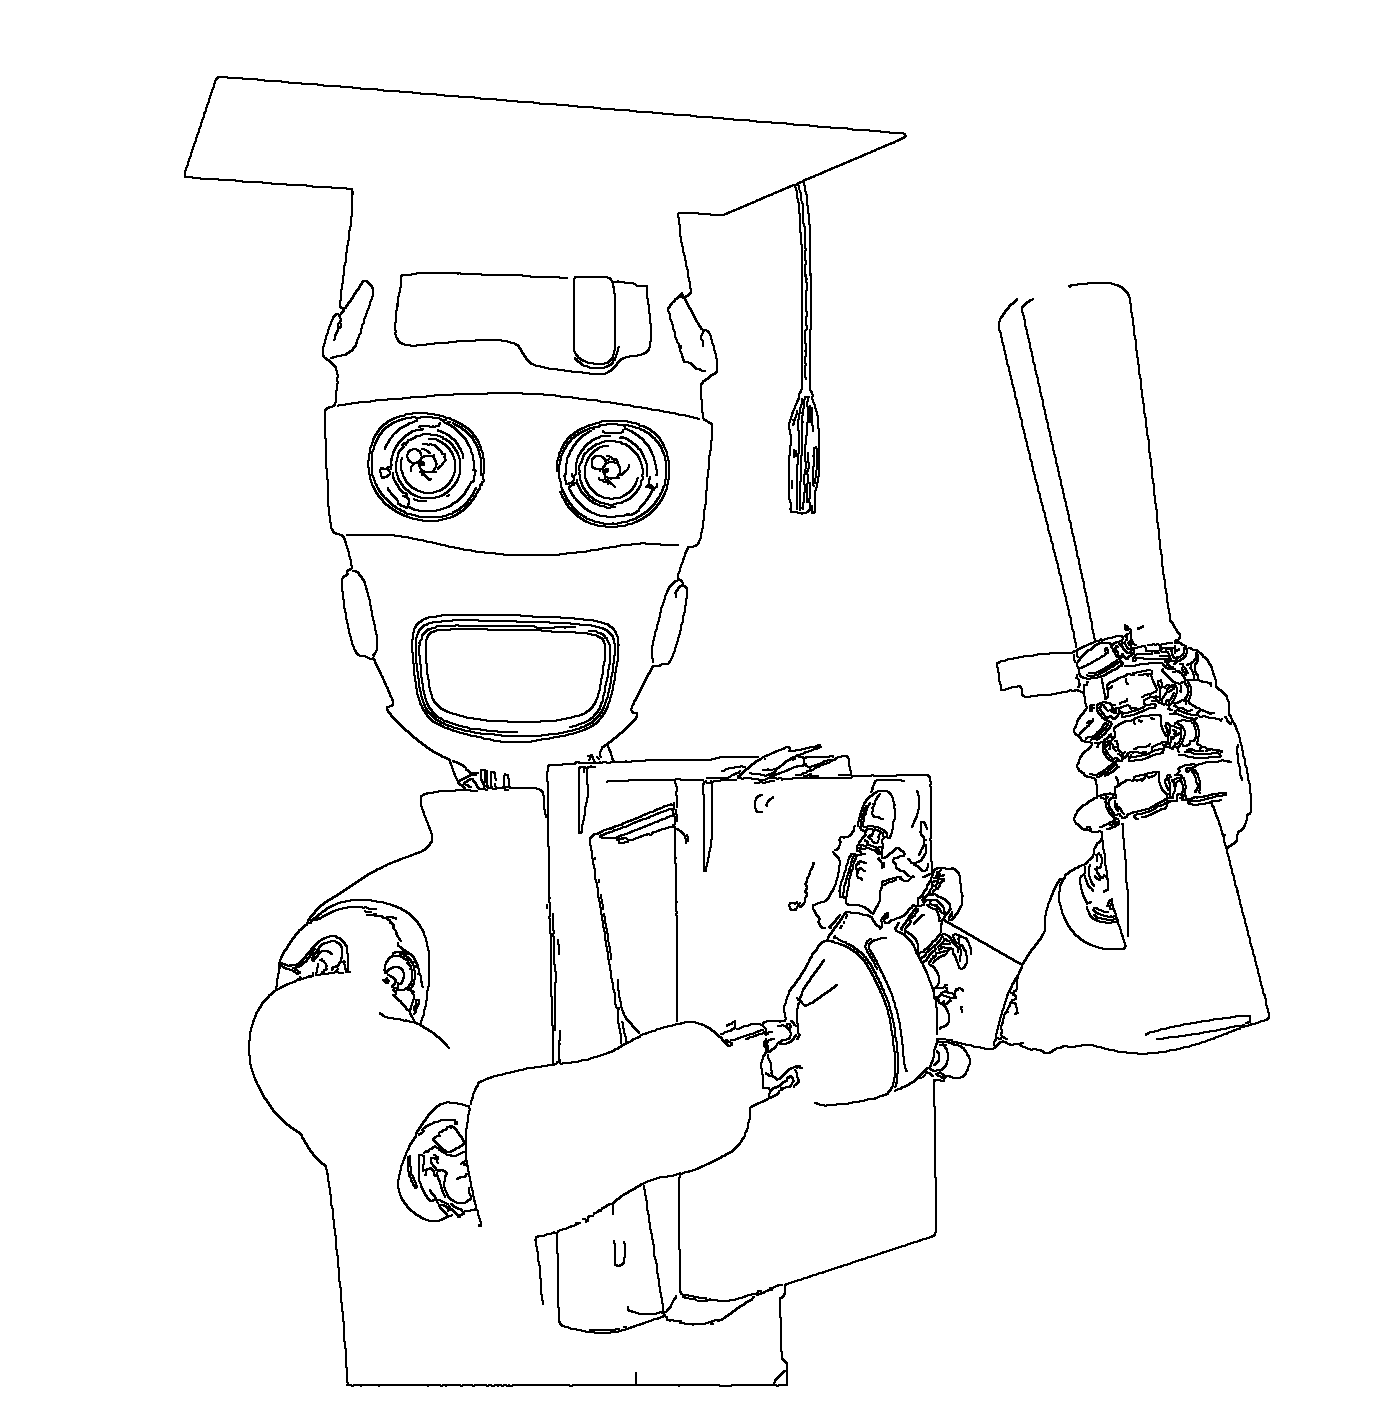
\includegraphics[width=0.6\linewidth]{figs/cover.png}
        \end{figure}
        \vfill
        
        {\large \textbf{Yifeng Xu}\\Harbin Institute of Technology, Shenzhen}\\[0.5cm]
        {\large 2020.12 -- 2021.02}
    \end{center}
\end{titlepage}

\thispagestyle{empty}
\newpage

\textbf{Course}

Machine Learning by Andrew Ng (Coursera)

\vspace{2ex}

\textbf{Lecturer}

Prof. Andrew Ng

\vspace{2ex}

\textbf{Slide}

GitHub: \url{https://github.com/TheisTrue/MLofAndrew-Ng}

\vspace{2ex}

\textbf{Online Video}

BiliBili: \url{https://www.bilibili.com/video/BV164411b7dx}
 \newpage
\tableofcontents \newpage
\section{梯度下降解一元线性回归}
\label{sec:chapter1}

\subsection{一元线性回归}

给定如下数据集：
\[
\left\{\left(x^{(i)},y^{(i)}\right),\;i=1,2,\cdots,m\right\}
\]
其中，$m$ 表示样本数量，$x^{(i)}$ 与 $y^{(i)}$ 分别表示第 $i$ 个样本的输入和对应的观测值。一元线性回归的目标是使用线性函数 $y=\theta_1x+\theta_0$ 对这些数据进行拟合。虽然该问题可以直接通过最小二乘法求得解析解，但本节以它为例介绍如何使用梯度下降法迭代求解。


\subsection{梯度下降法}

梯度下降法是一种常用的迭代优化算法。对于代价函数 $J(\theta_0,\theta_1)$，其基本思路是从一个初始参数点出发，沿当前点负梯度所指示的下降方向移动一小步，并反复执行这一过程，从而逐步减小代价函数的取值。若代价函数满足适当的凸性与光滑性条件，该过程可以收敛到其全局最小值；在更一般的情况下，梯度下降法通常用于寻找局部极小值或驻点。

函数 $J$ 关于参数 $\theta_0$ 和 $\theta_1$ 的梯度定义为：
\[
\text{grad }J=\left\{\frac{\partial J}{\partial \theta_0},\frac{\partial J}{\partial \theta_1}\right\}
\]
因此，可以按照下式不断更新参数：
\[
\theta_j:=\theta_j-\alpha\cdot\frac{\partial J}{\partial\theta_j},\quad j=0,1
\]
其中，$\alpha$ 表示每次更新的步长，通常称为\textbf{学习率}。需要注意的是，在一次迭代中，$\theta_0$ 和 $\theta_1$ 应当依据更新前的参数值同步计算并更新。

学习率的选取会直接影响算法的收敛速度和稳定性。学习率过小时，每次参数更新的幅度有限，因而收敛过程可能较慢；学习率过大时，参数则可能越过极小值附近的区域并反复振荡，甚至导致算法无法收敛。


\subsection{梯度下降解一元线性回归}

为了衡量模型预测值与真实观测值之间的差异，定义代价函数为：
\[
J(\theta_0,\theta_1)=\frac{1}{2m}\sum_{i=1}^m\left(\theta_1x^{(i)}+\theta_0-y^{(i)}\right)^2
\]
该函数是所有样本预测值与真实值的均方误差。

对代价函数分别关于 $\theta_0$ 和 $\theta_1$ 求偏导，可得：
\[
\text{grad }J=\left\{\frac{\partial J}{\partial \theta_0},\frac{\partial J}{\partial \theta_1}\right\}=\left\{\frac{1}{m}\sum_{i=1}^m\left(\theta_1x^{(i)}+\theta_0-y^{(i)}\right),\frac{1}{m}\sum_{i=1}^mx^{(i)}\left(\theta_1x^{(i)}+\theta_0-y^{(i)}\right)\right\}
\]
将上述两个偏导数代入参数更新公式，即可在每次迭代中沿负梯度方向调整 $\theta_0$ 和 $\theta_1$.


\subsection{代码实现}
\paragraph{C++ 实现}

对于该问题，可以预先计算样本中若干与参数无关的求和项，使每次梯度更新的时间复杂度降为 $O(1)$.

\begin{lstlisting}[language=C++]
#include<bits/stdc++.h>

using namespace std;

const double eps = 1e-8;
const double alpha = 0.01;

int m;
double sumx, sumy, sumxy, sumx2;
double th0, th1;

int main(){
	freopen("ex1data1.txt", "r", stdin);
	double x, y;
	while(scanf("%lf,%lf", &x, &y) != EOF)
		m++, sumx += x, sumy += y, sumx2 += x * x, sumxy += x * y;
	th0 = th1 = 0;
	while(1){
		double nth0, nth1;
		nth0 = th0 - alpha * 1.0 / m * (th1 * sumx - sumy + m * th0);
		nth1 = th1 - alpha * 1.0 / m * (th1 * sumx2 - sumxy + sumx * th0);
		if(fabs(th0 - nth0) < eps && fabs(th1 - nth1) < eps)	break;
		th0 = nth0, th1 = nth1;
	}
	printf("%f %f\n", th0, th1);
	return 0;
}
\end{lstlisting}

程序得到的结果为：$\theta_0=-3.895775,\,\theta_1=1.193033$.

若将 $\alpha$ 设为 $0.1$，上述程序将无法获得收敛结果。这是因为学习率过大，参数更新可能在极小值附近反复跨越，导致代价函数无法稳定下降。除直接减小 $\alpha$ 之外，还可以让程序根据迭代过程自适应地调整学习率。具体地，当学习率取值合理时，代价函数通常应当随迭代逐步减小。因此，如果一次参数更新后代价函数反而增大，就可以将其视为当前学习率过大的信号，并相应减小 $\alpha$。基于这一思路，可以得到如下实现：

\begin{lstlisting}[language=C++]
#include<bits/stdc++.h>

using namespace std;

const int N = 105;
const double eps = 1e-8;
double alpha = 100;

int m;
double x[N], y[N];
double th0, th1;

inline double gradJ(int k){
	double res = 0;
	for(int i = 1; i <= m; i++)
		res += (th1 * x[i] + th0 - y[i]) * (k == 1 ? x[i] : 1);
	return res / m;
}

inline double calc(){
	double res = 0;
	for(int i = 1; i <= m; i++)
		res += (th1 * x[i] + th0 - y[i]) * (th1 * x[i] + th0 - y[i]);
	return res / m / 2;
}

int main(){
	freopen("ex1data1.txt", "r", stdin);
	while(scanf("%lf,%lf", &x[0], &y[0]) != EOF)
		m++, x[m] = x[0], y[m] = y[0];
	th0 = th1 = 0;
	double preJ = 1e9, J = 0;
	while(1){
		double nth0, nth1;
		nth0 = th0 - alpha * gradJ(0);
		nth1 = th1 - alpha * gradJ(1);
		if(fabs(th0 - nth0) < eps && fabs(th1 - nth1) < eps)	break;
		th0 = nth0, th1 = nth1;
		J = calc();
		if(J > preJ)	alpha /= 5;
		preJ = J;
	}
	printf("%f\n%f %f\n", alpha, th0, th1);
	return 0;
}
\end{lstlisting}

最终得到的结果为：$\alpha=0.0064,\,\theta_0=-3.895772,\,\theta_1=1.193033$.


\paragraph{Python 实现}

Python 拥有较为完善的可视化工具，常用于机器学习算法的实现和实验分析。
如下是学习率设置为 0.01 的 Python 代码：

\begin{lstlisting}[language=Python]
import numpy as np
import matplotlib.pyplot as plt

X = []
Y = []
m = 0
alpha = 0.01
eps = 1e-8
th0, th1 = 0, 0

def gradJ(k):
	res = 0
	for x, y in zip(X, Y):
		res += (th1 * x + th0 - y) * (x if k == 1 else 1)
	return res / m

def calc():
	res = 0
	for x, y in zip(X, Y):
		res += (th1 * x + th0 - y) * (th1 * x + th0 - y)
	return res / 2 / m

with open("ex1data1.txt", "r") as infile:
	data = infile.readlines()
	for line in data:
		x, y = line.split(',')
		X.append(float(x))
		Y.append(float(y))
		m += 1


while 1:
	nth0 = th0 - alpha * gradJ(0)
	nth1 = th1 - alpha * gradJ(1)
	if abs(th0 - nth0) < eps and abs(th1 - nth1) < eps:
		break
	th0 = nth0
	th1 = nth1
print(th0, th1)
plt.scatter(X, Y)
plt.plot([min(X), max(X)], [th0+min(X)*th1, th0+max(X)*th1], c="magenta")
plt.show()
\end{lstlisting}

程序得到的结果为：$\theta_0=-3.895775,\,\theta_1=1.193033$，原始数据及拟合效果如下图所示：

\begin{figure}[H]
    \centering
    \begin{minipage}{0.4\linewidth}
        \centering
        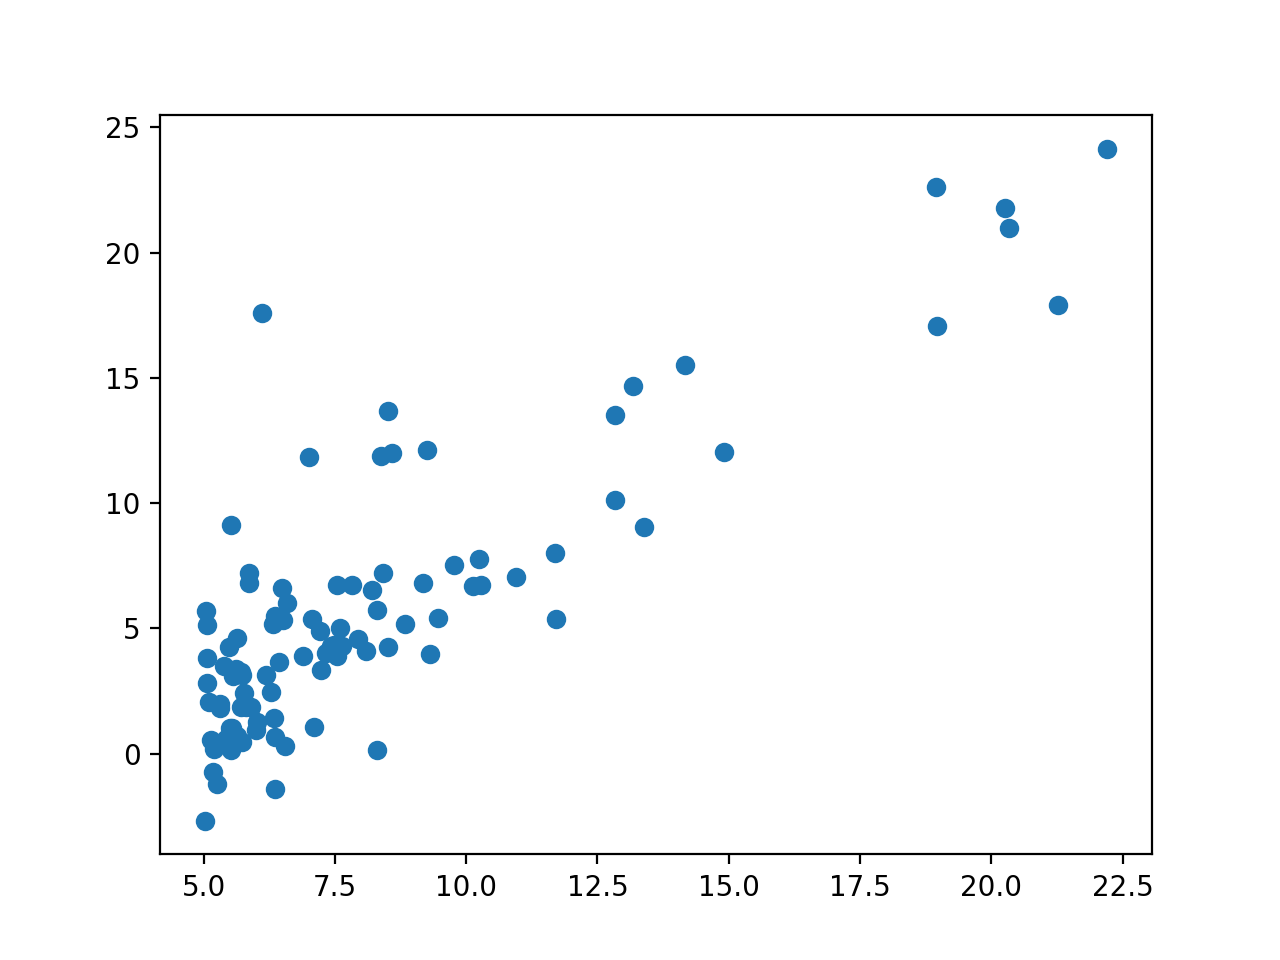
\includegraphics[width=\linewidth]{figs/Chap_1_Figure_1.png}
    \end{minipage}
    \begin{minipage}{0.4\linewidth}
        \centering
        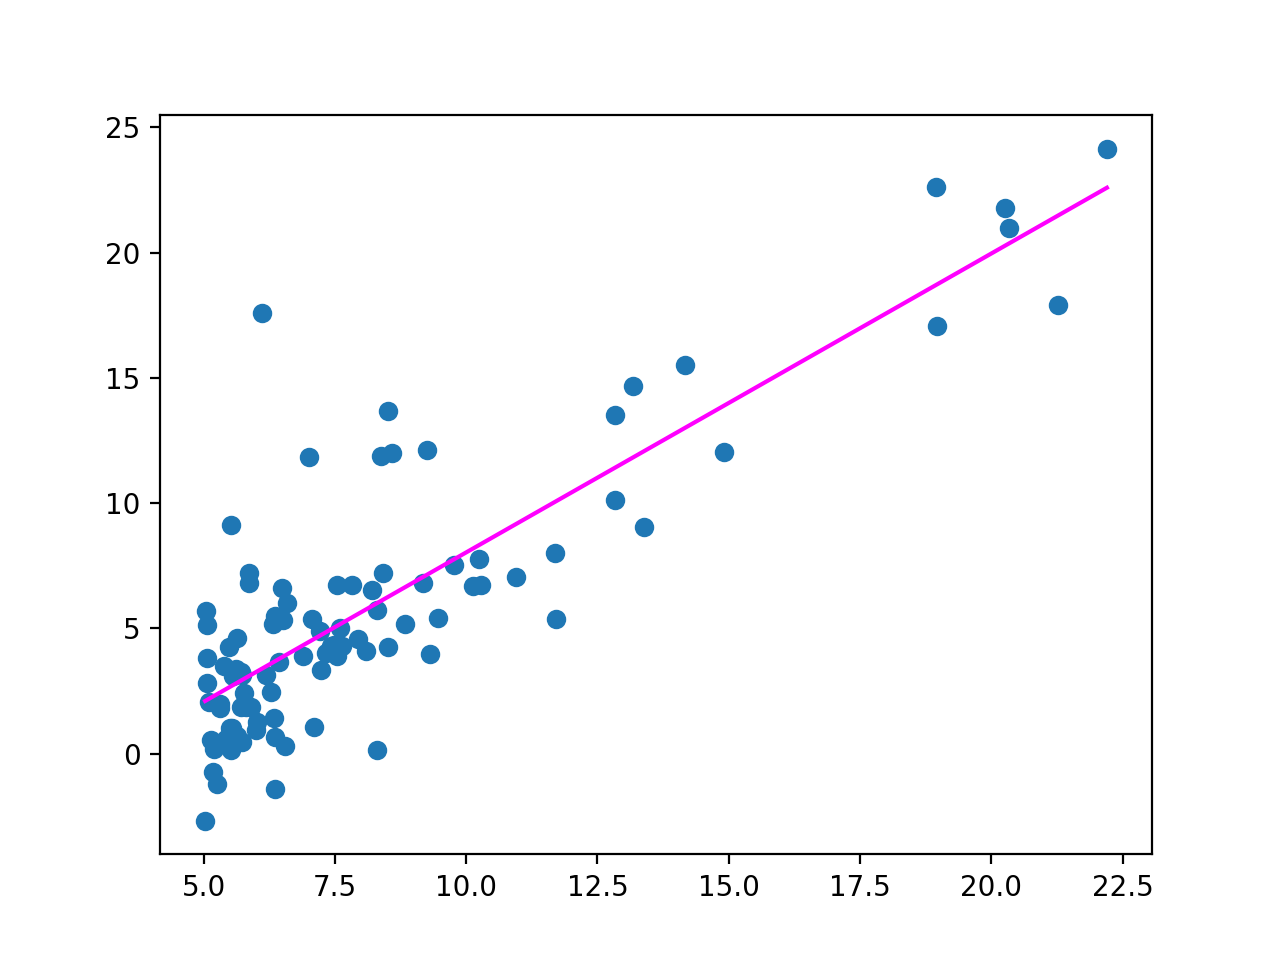
\includegraphics[width=\linewidth]{figs/Chap_1_Figure_2.png}
    \end{minipage}
    \vspace{-2ex}
\end{figure}

图中的洋红色直线即为梯度下降法得到的线性回归模型。

前文已经指出，学习率过大会导致迭代无法收敛，即 $J(\theta_0,\theta_1)$ 可能随迭代次数增加而增大。为了比较不同学习率对收敛过程的影响，可以绘制代价函数随迭代次数变化的曲线：

\begin{figure}[H]
    \centering
    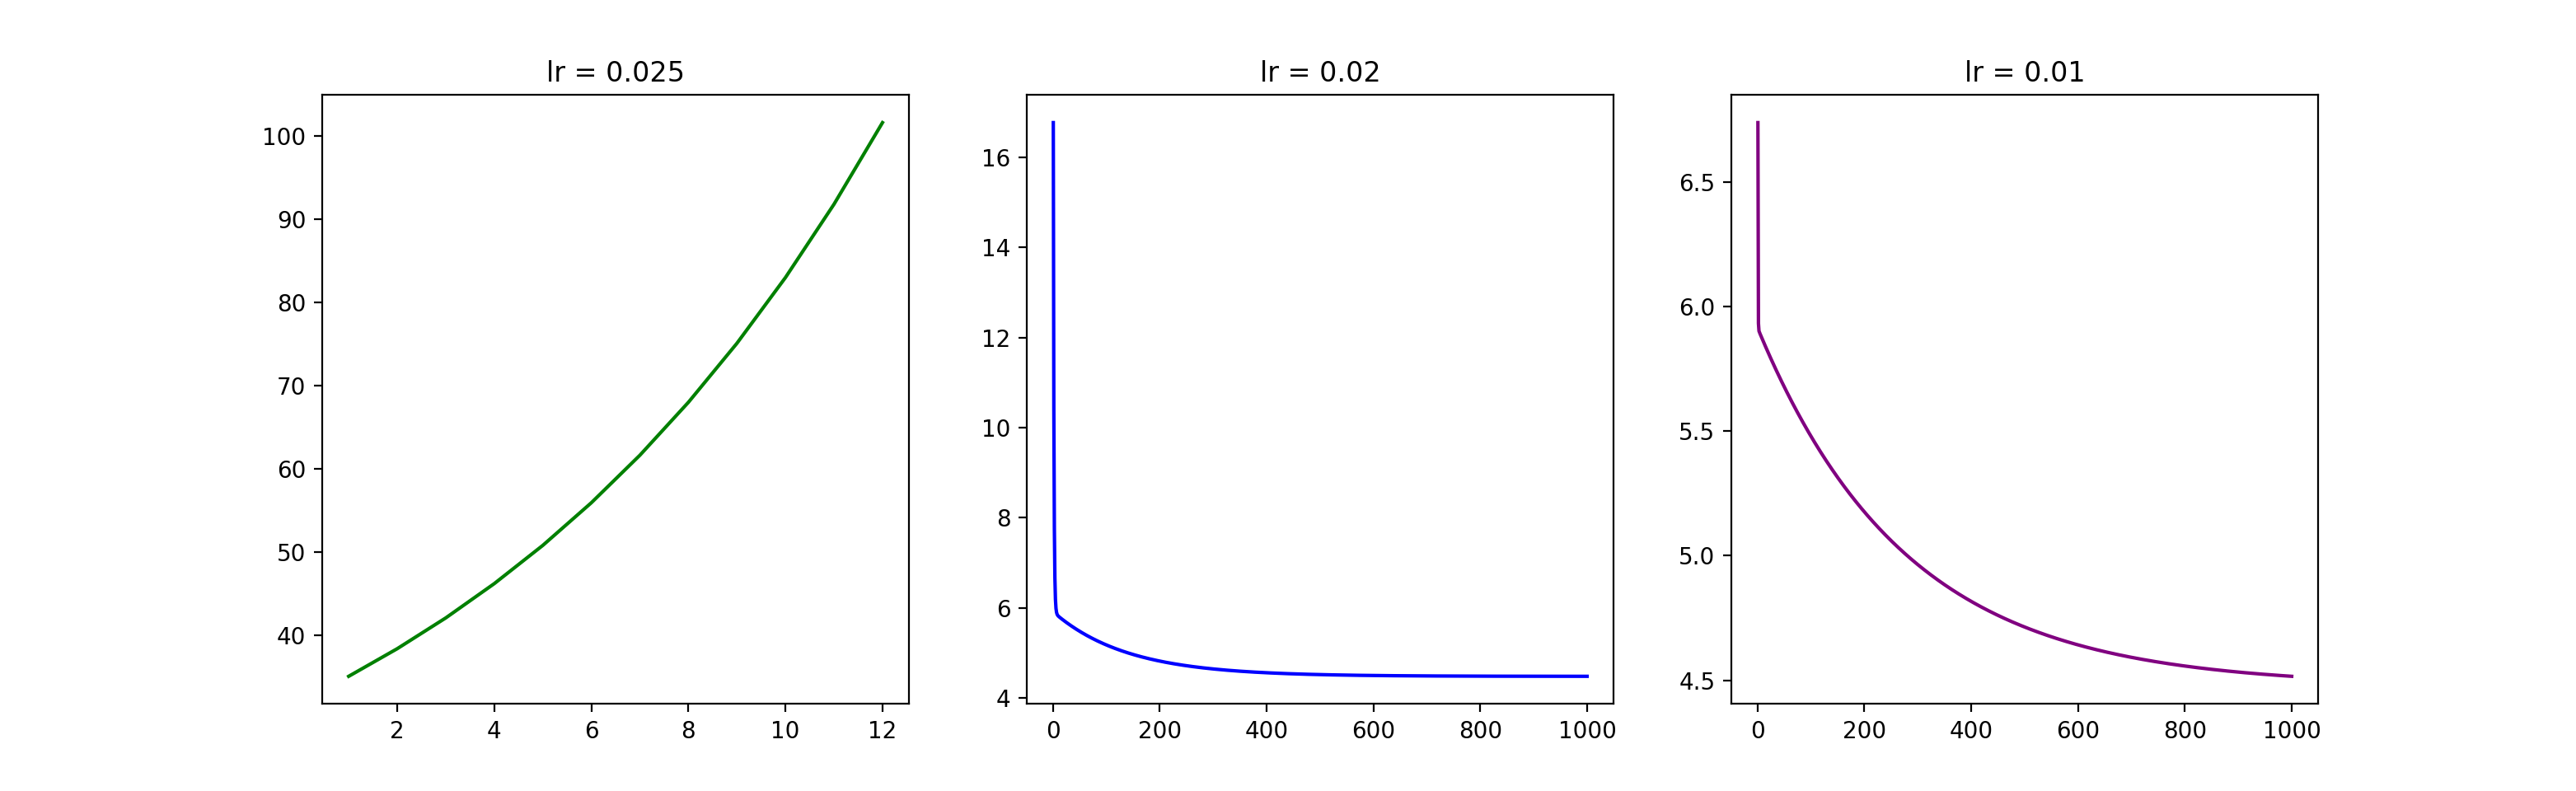
\includegraphics[width=\linewidth]{figs/Chap_1_Figure_3.png}
    \vspace{-3ex}
\end{figure}

由图可见，当学习率为 $0.025$ 时，代价函数呈发散趋势；当学习率分别为 $0.02$ 和 $0.01$ 时，代价函数能够逐步收敛。这一结果说明，学习率需要结合具体问题进行选择，适当的取值才能兼顾收敛速度与迭代稳定性。
 \newpage
\section{梯度下降解多元线性回归}
\label{sec:chapter2}

\subsection{多元线性回归}

类似于一元的线性回归，不过我们现在有多个自变量 $x_1,x_2,\cdots,x_n$，即给定的数据集为：
\[
\left\{\left(x_1^{(i)},x_2^{(i)},\cdots,x_n^{(i)},y^{(i)}\right),\;i=1,2,\cdots,m\right\}
\]
相应地，回归方程也具有多个参数 $\theta_0,\theta_1,\cdots,\theta_n$：
\[
h_\theta(x)=\theta^Tx=\theta_0x_0+\cdots+\theta_nx_n
\]
这里我们假定 $x_0$ 恒等于 $1$，并以向量表示自变量和参数：$\theta=(\theta_0,\cdots,\theta_n)^T,\;x=(x_0,\cdots,x_n)^T$. 



\subsection{梯度下降解多元线性回归}

类似的，我们定义代价函数：
\[
J(\theta)=\frac{1}{2m}\sum_{i=1}^m\left(\theta^Tx^{(i)}-y^{(i)}\right)^2
\]
于是，
\[
\frac{\partial J}{\partial \theta}=\frac{1}{m}\sum_{i=1}^m\left(\theta^Tx^{(i)}-y^{(i)}\right)x^{(i)}
\]
梯度下降时，不断作迭代：
\[
\theta:=\theta-\alpha\cdot\frac{\partial J}{\partial \theta}
\]
即可。


\paragraph{特征缩放与标准化}

当我们的不同自变量取值范围相差较大时，梯度下降可能会很慢，这时，我们需要把所有自变量进行缩放、标准化。具体的，只要我们置：
\[
x_i^{(j)}:=\frac{x_i^{(j)}-\mu_i}{\sigma_i}
\]
其中，$\mu_i=\frac{1}{m}\sum\limits_{j=1}^m x_i^{(j)}$ 是样本均值，$\sigma_i=\sqrt{\frac{\sum\limits_{j=1}^m\left(x_i^{(j)}-\mu_i\right)^2}{m-1}}$ 是样本标准差，就完成了归一化。

归一化后样本均值为 $0$，方差为 $1$. 


\paragraph{代码实现}

\texttt{Normalization} 函数将数据集标准化，\texttt{J} 函数即计算 $J(\theta)$，\texttt{partJ} 函数计算 $\frac{\partial J}{\partial\theta}$，\texttt{GradientDescent} 进行梯度下降。

\begin{lstlisting}[language=Python]
import numpy as np
import matplotlib.pyplot as plt

alpha = 0.01
iteration = 10000
Z = []

def Normalization(data):
	return (data - data.mean(axis = 0)) / data.std(axis = 0, ddof = 1)

def J(T, X, Y):
	res = 0
	for i in range(m):
		res += (np.matmul(T.T, X[i:i+1, :].T) - Y[i:i+1, :]) ** 2
	res /= 2 * m;
	return res

def partJ(T, X, Y):
	res = np.zeros((n, 1))
	for i in range(m):
		res += (np.matmul(T.T, X[i:i+1, :].T) - Y[i:i+1, :]) * X[i:i+1, :].T
	res /= m
	return res

def GradientDescent(X, Y):
	T = np.zeros((n, 1))
	for t in range(iteration):
		T = T - alpha * partJ(T, X, Y)
		Z.append(J(T, X, Y)[0][0])
	return T

data = np.genfromtxt("ex1data2.txt", delimiter = ',')
(m, n) = data.shape
data = Normalization(data)
X = np.column_stack((np.ones((m, 1)), data[:, :-1]))
Y = data[:, -1:]
T = GradientDescent(X, Y)
print(T)

p1 = plt.subplot(111)
p1.plot(range(1, iteration+1), Z)
p1.set_xlabel('Iteration')
p1.set_ylabel('Cost')
plt.show()
\end{lstlisting}

最后得到的结果：$\theta=(-1.11051830\times10^{-16},8.84765988\times10^{-1},-5.31788197\times10^{-2})^T$. 

学习率取为 $0.01$ 时，代价函数值随迭代次数的变化：

\begin{figure}[H]
    \centering
    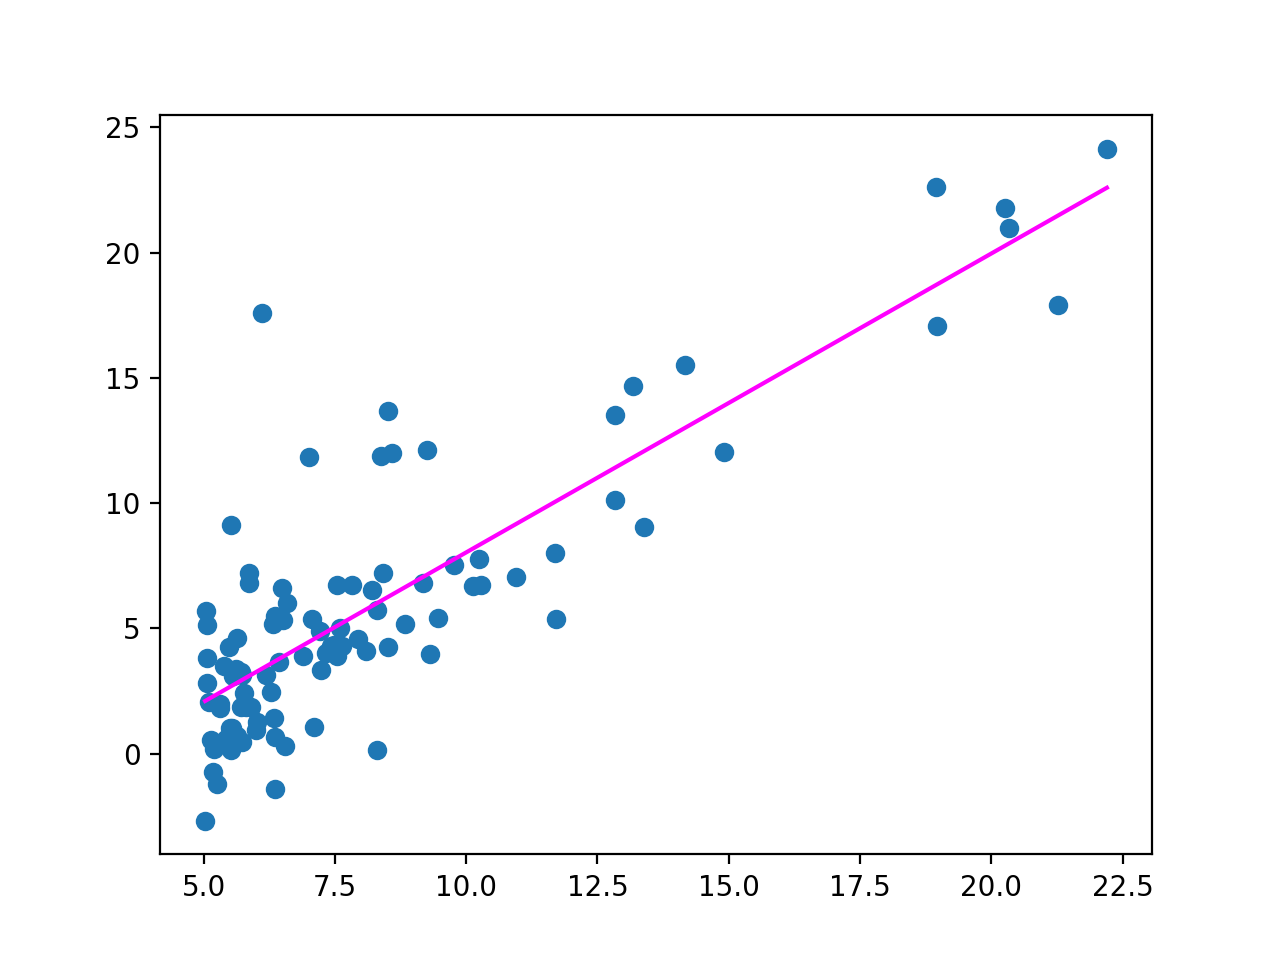
\includegraphics[width=0.5\linewidth]{figs/Chap_1_Figure_2.png}
\end{figure} \newpage
\section{正规方程解多元线性回归}
\label{sec:chapter3}

\subsection{正规方程}

正规方程利用多元微分直接求解线性回归的最优参数，无须像梯度下降那样反复迭代。

对于代价函数：
\[
J(\theta)=J(\theta_0, \theta_1,\cdots, \theta_n)
\]
若代价函数可微且为凸函数，则可令各偏导数为零，从而求得使其取最小值的参数 $\theta$：
\[
\frac{\partial J}{\partial \theta_j}=0,\quad j=0,1,\cdots,n
\]
写成向量形式即为：
\[
\frac{\partial J}{\partial \theta}=\vec 0
\]
下面将这一方法应用于多元线性回归。

多元线性回归的代价函数为：
\[
J(\theta)=\frac{1}{2m}\sum_{i=1}^m\left(\theta^Tx^{(i)}-y^{(i)}\right)^2
\]
其梯度为：
\[
\frac{\partial J}{\partial \theta}=\frac{1}{m}\sum_{i=1}^m\left(\theta^Tx^{(i)}-y^{(i)}\right)x^{(i)}
\]
令其为零，解得：
\[
\theta^Tx^{(i)}=y^{(i)},\quad i=1,2,\cdots,m
\]
这些等式可以统一写成矩阵形式：
\[
X\theta=y
\]
其中，
\[
X=\begin{bmatrix}x_0^{(1)}&x_1^{(1)}&\cdots& x_n^{(1)}\\x_0^{(2)}&x_1^{(2)}&\cdots& x_n^{(2)}\\\vdots&\vdots&\ddots&\vdots\\x_0^{(m)}&x_1^{(m)}&\cdots& x_n^{(m)}\end{bmatrix}=\begin{bmatrix}{x^{(1)}}^T\\{x^{(2)}}^T\\\vdots\\{x^{(m)}}^T\\\end{bmatrix},\quad y=\begin{bmatrix}y^{(1)}\\y^{(2)}\\\vdots\\y^{(m)}\end{bmatrix}
\]
两边同时乘以 $X^T$，并假设 $X^TX$ 可逆，解得：
\[
\theta=(X^TX)^{-1}X^Ty
\]
这就是多元线性回归的解析解。

由于 $X^TX$ 是一个 $(n+1)\times(n+1)$ 的矩阵，直接求逆或求解线性方程组的时间复杂度通常为 $O(n^3)$. 当 $n$ 不大时，正规方程能够一次得到解析解，也不需要选择学习率；但当 $n$ 达到 $10^4,10^5$ 或更高数量级时，矩阵运算的时间和空间开销都会迅速增加，此时通常应考虑梯度下降等迭代方法。


\subsection{代码实现}

仍使用第 \ref{sec:chapter2} 节中的多元线性回归数据，代码如下：

\begin{lstlisting}[language=Python]
import numpy as np

def J(T, X, Y):
	res = 0
	for i in range(m):
		res += (np.matmul(T.T, X[i:i+1, :].T) - Y[i:i+1, :]) ** 2
	res /= 2 * m;
	return res

data = np.genfromtxt("ex1data2.txt", delimiter = ',')
(m, n) = data.shape
X = np.column_stack((np.ones((m, 1)), data[:, :-1]))
Y = data[:, -1:]
T = np.matmul(np.matmul(np.linalg.inv(np.matmul(X.T, X)), X.T), Y)
print(T)
print(J(T, X, Y))
\end{lstlisting}

计算很快即可完成，结果为：$\theta=(89597.9095428,\,139.21067402,\,-8738.01911233)^T$.


\subsection{不可逆情形}

上述求解过程建立在 $X^TX$ 可逆的假设上。当特征之间存在冗余或线性相关关系时，该矩阵可能不可逆。此时可以将代码中的 \texttt{inv()} 替换为 \texttt{pinv()}，通过\textbf{伪逆矩阵}求得一个最小二乘意义下的解。

\begin{lstlisting}[language=Python]
import numpy as np

def J(T, X, Y):
	res = 0
	for i in range(m):
		res += (np.matmul(T.T, X[i:i+1, :].T) - Y[i:i+1, :]) ** 2
	res /= 2 * m;
	return res

data = np.genfromtxt("ex1data2.txt", delimiter = ',')
(m, n) = data.shape
X = np.column_stack((np.ones((m, 1)), data[:, :-1]))
Y = data[:, -1:]
T = np.matmul(np.matmul(np.linalg.pinv(np.matmul(X.T, X)), X.T), Y)
print(T)
print(J(T, X, Y))
\end{lstlisting}
 \newpage
\section{逻辑回归之二分类}
\label{sec:chapter4}

\subsection{二分类问题与逻辑回归的引入}

给定数据集：
\[
\left\{\left(x^{(i)},y^{(i)}\right),\;i=1,2,\cdots,m\right\}
\]
其中 $x^{(i)}$ 是一个 $n$ 维向量 $\left(x_0^{(i)},\cdots,x_n^{(i)}\right)^T$，且 $y^{(i)}\in\{0,1\}$，也即是对于输入 $x^{(i)}$，我们将其分类为 $0$ 或 $1$ 两类。试用一模型拟合该分类结果。

鉴于 $y$ 取值的离散性，线性回归在这里不好使了，我们引入逻辑回归的概念。

回忆线性回归的假设函数：$h_\theta(x)=\theta^Tx$，我们在其外套上 $\text{sigmoid}$ 函数，构造逻辑回归的假设函数为：
\[
h_\theta(x)=g\left(\theta^Tx\right)=\frac{1}{1+e^{-\theta^T x}}
\]

\begin{note}
$\text{sigmoid}$ 函数：
\[
g(z)=\frac{1}{1+e^{-z}}
\]
是一个介于 $(0,1)$ 之间的单增 $S$ 形函数。
\end{note}

也就是说，对于一个参数为 $\theta$ 的逻辑回归模型，输入 $x$，得到 $h_\theta(x)=\frac{1}{1+e^{-\theta^Tx}}$ 的预测。我们可以把这个值视为 $x$ 这组数据对应的 $y$ 等于 $1$ 的概率，如果它 $\geqslant 0.5$，则分类为 $1$，否则分类为 $0$. 

又根据 $\text{sigmoid}$ 函数的性质，$h_\theta(x)\geqslant 0.5\iff \theta^Tx\geqslant0$. 所以只要 $\theta^Tx\geqslant0$，就分类为 $1$，否则分类为 $0$；于是乎，$\theta^Tx=0$ 这条线（超平面）被称作决策边界，它将整个空间划分成两块，各自属于一个分类。


\subsection{代价函数}

现在，我们的任务就是从数据集中求解逻辑回归的参数 $\theta$. 仍然采用代价函数的思想——找到使代价最小的参数即可。

广义上来讲，代价函数是这样的一个函数：
\[
J(\theta)=\frac{1}{m}\sum_{i=1}^m\text{Cost}\left(h_\theta(x^{(i)}),y^{(i)}\right)
\]
也就是说用每个数据的估计值 $h_\theta(x^{(i)})$ 和真实值 $y^{(i)}$ 计算一个代价 $\text{Cost}\left(h_\theta(x^{(i)}),y^{(i)}\right)$，比如线性回归中这个代价就是二者差值的平方。

具体到逻辑回归里，这个代价定义为：
\begin{align*}
\text{Cost}\left(h_\theta(x),y\right)&=\begin{cases}-\ln(h_\theta(x))&y=1\\-\ln(1-h_\theta(x))&y=0\end{cases}\\
&=-y\ln(h_\theta(x))-(1-y)\ln(1-h_\theta(x))\\
&=y\ln\left(1+e^{-\theta^Tx}\right)+(1-y)\ln\left(1+e^{\theta^Tx}\right)
\end{align*}

\begin{proof}
上式的来源：

前文已经提到，$h_\theta(x)=\mathbb P(y=1)$，于是 $1-h_\theta(x)=\mathbb P(y=0)$，故：
\[
\mathbb P(y=k)=[h_\theta(x)]^k[1-h_\theta(x)]^{1-k},\quad k\in\{0,1\}
\]
考虑\textbf{极大似然法}，在数据集 $\left\{\left(x^{(i)},y^{(i)}\right),\;i=1,2,\cdots,m\right\}$ 下，似然函数为：
\[
L(\theta)=\prod_{i=1}^m\mathbb P\left(y=y^{(i)}\right)=\prod_{i=1}^m\left[h_\theta(x^{(i)})\right]^{y^{(i)}}\left[1-h_\theta(x^{(i)})\right]^{1-y^{(i)}}
\]
取对数得到：
\[
\ln L(\theta)=\sum_{i=1}^my^{(i)}\ln(h_\theta(x^{(i)}))+(1-y^{(i)})\ln(1-h_\theta(x^{(i)}))
\]
注意到，极大似然法的目标是找到 $L(\theta)$ 或 $\ln L(\theta)$ 的极大值，而逻辑回归的目标是找到 $J(\theta)$ 的极小值，所以自然的，我们直接使用 $\ln L(\theta)$ 来定义 $J(\theta)$：
\[
J(\theta)=-\frac{1}{m}\ln L(\theta)
\]
这个 $\frac{1}{m}$ 对极大值/极小值没有影响，仅是取一下平均罢了。

换句话说，\textbf{逻辑回归的本质是拟合 $y$ 取值的概率，并以极大似然法解之}。
\end{proof}


\subsection{梯度下降解逻辑回归}

我们对逻辑回归定义的代价函数是非常好的：它是一个凸函数。这有助于我们进行梯度下降求解。

为了求偏导，我们先计算：
\begin{align*}
\frac{\partial}{\partial\theta}\text{Cost}(h_\theta(x), y)&=\frac{\partial}{\partial \theta}\left[y\ln\left(1+e^{-\theta^Tx}\right)+(1-y)\ln\left(1+e^{\theta^Tx}\right)\right]\\
&=\frac{-yxe^{-\theta^Tx}}{1+e^{-\theta^Tx}}+\frac{(1-y)xe^{\theta^T x}}{1+e^{\theta^T x}}\\
&=\frac{-yx+(1-y)xe^{\theta^Tx}}{1+e^{\theta^Tx}}\\
&=\left(-y+\frac{1}{1+e^{-\theta^Tx}}\right)x\\
&=(h_\theta(x)-y)x
\end{align*}
于是乎，
\[
\frac{\partial J}{\partial\theta}=\frac{1}{m}\sum_{i=1}^m\left(h_\theta(x^{(i)})-y^{(i)}\right)x^{(i)}
\]
没错，这个偏导的形式和线性回归的偏导形式完全相同！不同的只是 $h_\theta(x)$ 的定义——逻辑回归的假设函数在线性回归的假设函数外套了一层 $\text{sigmoid}$ 函数，也正是这一层 $\text{sigmoid}$ 函数，让我们不能像线性回归那样直接给出解析解，而必须使用梯度下降等方法。

现在我们对其使用梯度下降即可。


\subsection{代码实现}

首先看一下数据的散点图：

\begin{figure}[H]
    \centering
    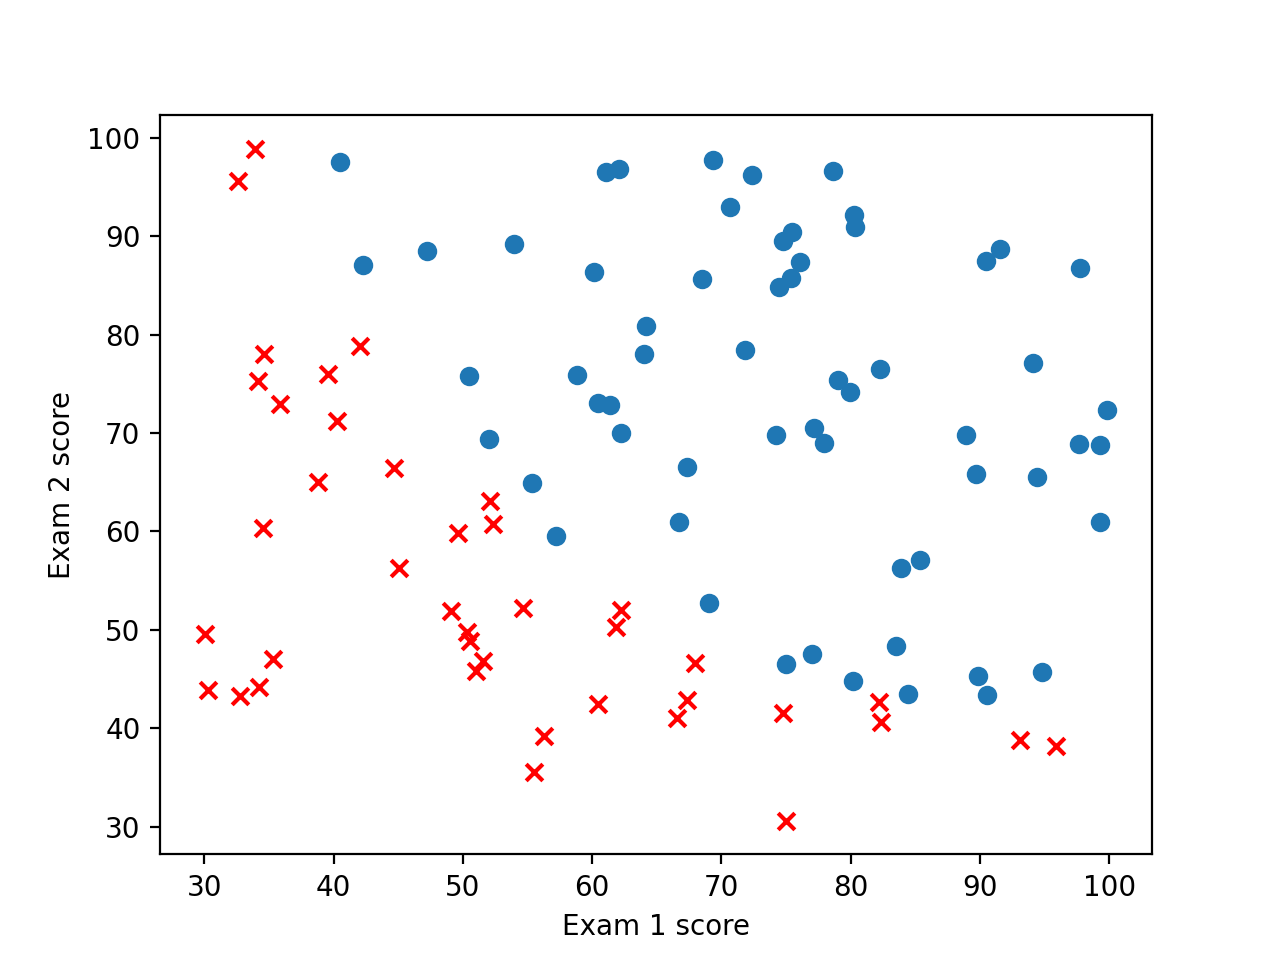
\includegraphics[width=0.5\linewidth]{figs/Chap_4_Figure_1.png}
\end{figure}

python 实现逻辑回归如下：

\begin{lstlisting}[language=Python]
import numpy as np
import matplotlib.pyplot as plt
import math

alpha = 0.01
iteration = 10000
Z = []

def Normalization(data):
	return (data - data.mean(axis = 0)) / data.std(axis = 0, ddof = 1)

def h(T, x):
	return 1 / (1 + np.e ** (-np.matmul(T.T, x)[0][0]))

def J(T, X, Y):
	res = 0
	for i in range(m):
		res -= Y[i] * math.log(h(T, X[i:i+1, :].T)) + \
		(1 - Y[i]) * math.log(1 - h(T, X[i:i+1, :].T))
	res /= m
	return res

def partJ(T, X, Y):
	res = np.zeros((n, 1))
	for i in range(m):
		res += (h(T, X[i:i+1, :].T) - Y[i]) * X[i:i+1, :].T
	res /= m
	return res

def GradientDescent(X, Y):
	T = np.zeros((n, 1))
	for t in range(iteration):
		T = T - alpha * partJ(T, X, Y)
		Z.append(J(T, X, Y))
	return T

data = np.genfromtxt("ex2data1.txt", delimiter = ',')
(m, n) = data.shape
data[:, :-1] = Normalization(data[:, :-1])
X = np.column_stack((np.ones((m, 1)), data[:, :-1]))
Y = data[:, -1]
T = GradientDescent(X, Y)
print(T)
print(J(T, X, Y))

p1 = plt.subplot(111)
p1.plot(range(1, iteration+1), Z)
p1.set_xlabel("Iteration")
p1.set_ylabel("Cost")
plt.show()
\end{lstlisting}

在学习率为 $0.01$ 下迭代了 $10000$ 次，结果为：$\theta=(1.2677702,\,3.05550587,\,2.81891901)^T$，此时 $J(\theta)=0.21065763610049573$. 决策边界的图像为：

\begin{figure}[H]
    \centering
    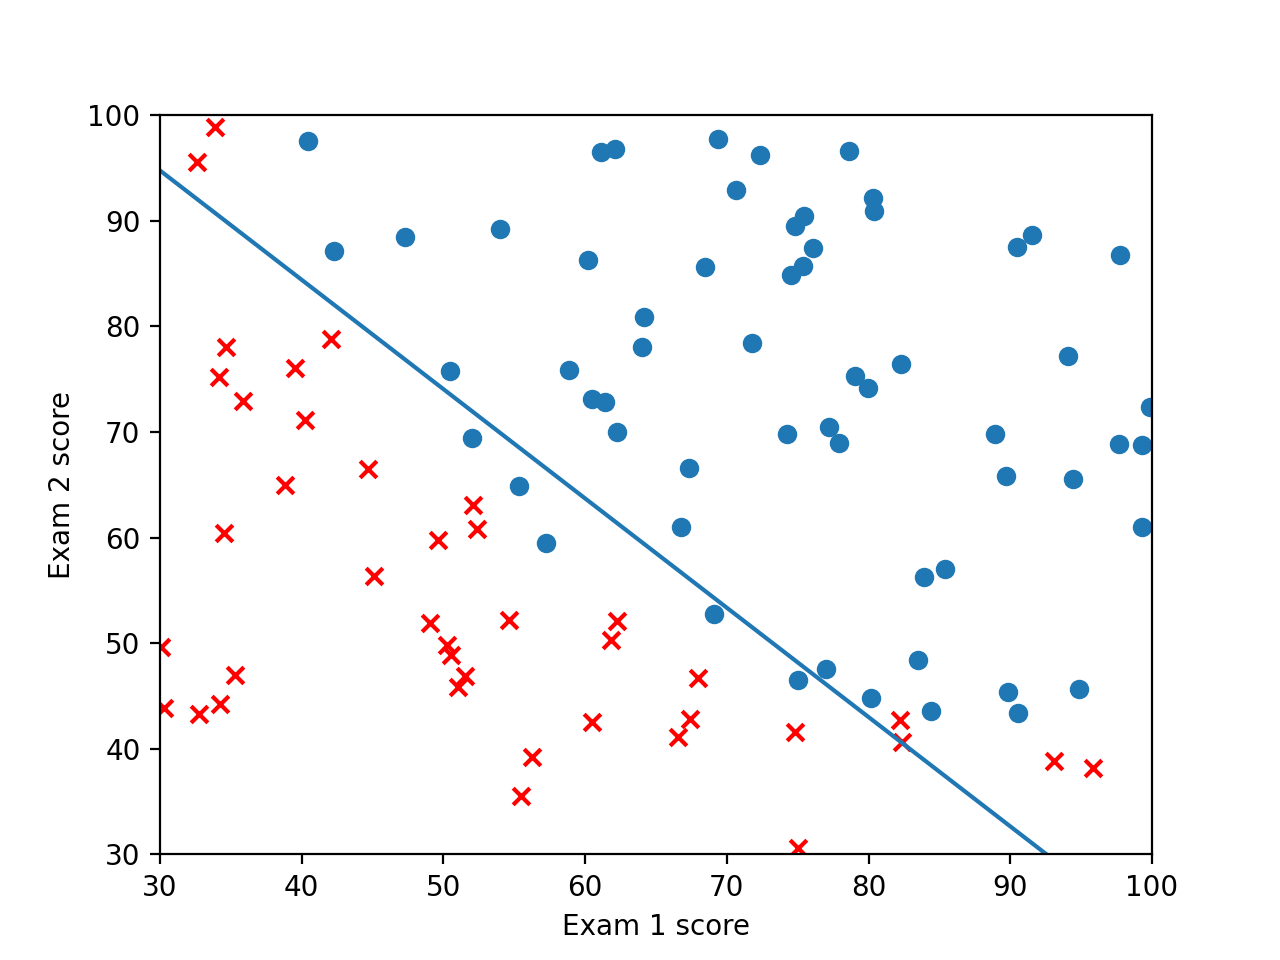
\includegraphics[width=0.5\linewidth]{figs/Chap_4_Figure_3.png}
\end{figure}

$J(\theta)$ 随迭代次数收敛情况如下：

\begin{figure}[H]
    \centering
    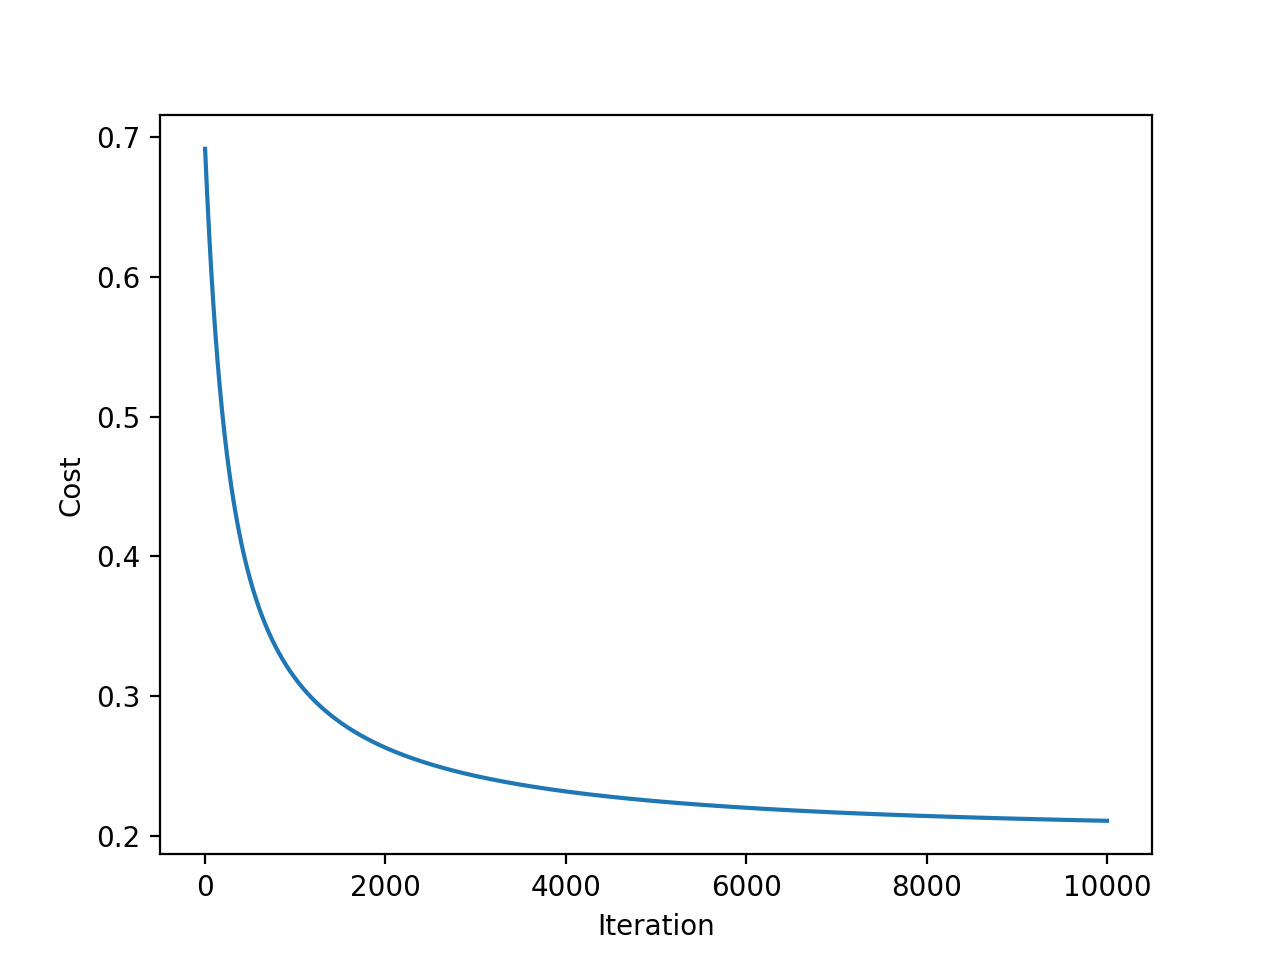
\includegraphics[width=0.5\linewidth]{figs/Chap_4_Figure_2.png}
\end{figure}
 \newpage
\section{正则化}
\label{sec:chapter5}

\subsection{过拟合}

以多项式回归为例。多项式回归是指在线性回归的基础上，人为的引入高阶项并将其视为新的一维特征，然后进行线性回归，从而达到拟合非线性数据的目的。举例而言，设线性回归的一个数据是 $\left(x^{(i)},y^{(i)}\right)$，我们在多项式回归时可以将其视为 $\left(x^{(i)},{x^{(i)}}^2,y^{(i)}\right)$，这样就人为引入了一个二阶项，我们的回归方程（假设函数）就变成了：$y=\theta_0+\theta_1x+\theta_2x^2$，如此就用二次函数去拟合数据了。

我们知道，一个函数可以泰勒展开成幂级数，越展开幂级数越接近原函数，那在回归中是不是也是次数越高越好呢？答案是否定的，因为我们只有有限个数据。如果特征维数 $n$ 过于接近数据量 $m$，则它会很好地拟合上我们的数据集，然而对于不在数据集中的数据，这可能并不是一个好的拟合结果。譬如，$n=m$ 时，由插值的原理容易知道，我们可以找到一个唯一的 $n-1$ 次多项式完美地经过所有数据，即每个数据集中的数据偏差都是 $0$，但是这显然不是一个好的拟合，如下图：

\begin{figure}[H]
    \centering
    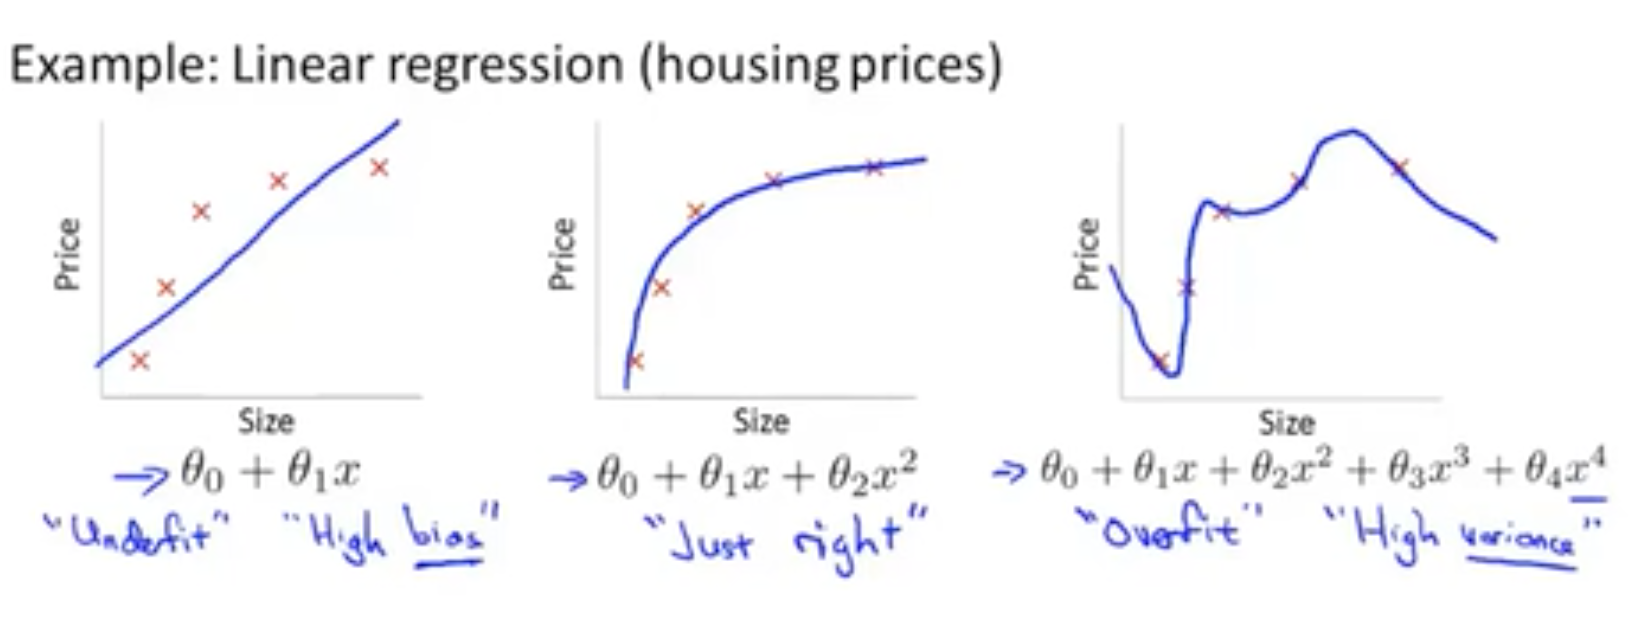
\includegraphics[width=0.8\linewidth]{figs/Chap_5_img1.png}
\end{figure}

同样地，逻辑回归也可能产生过拟合：

\begin{figure}[H]
    \centering
    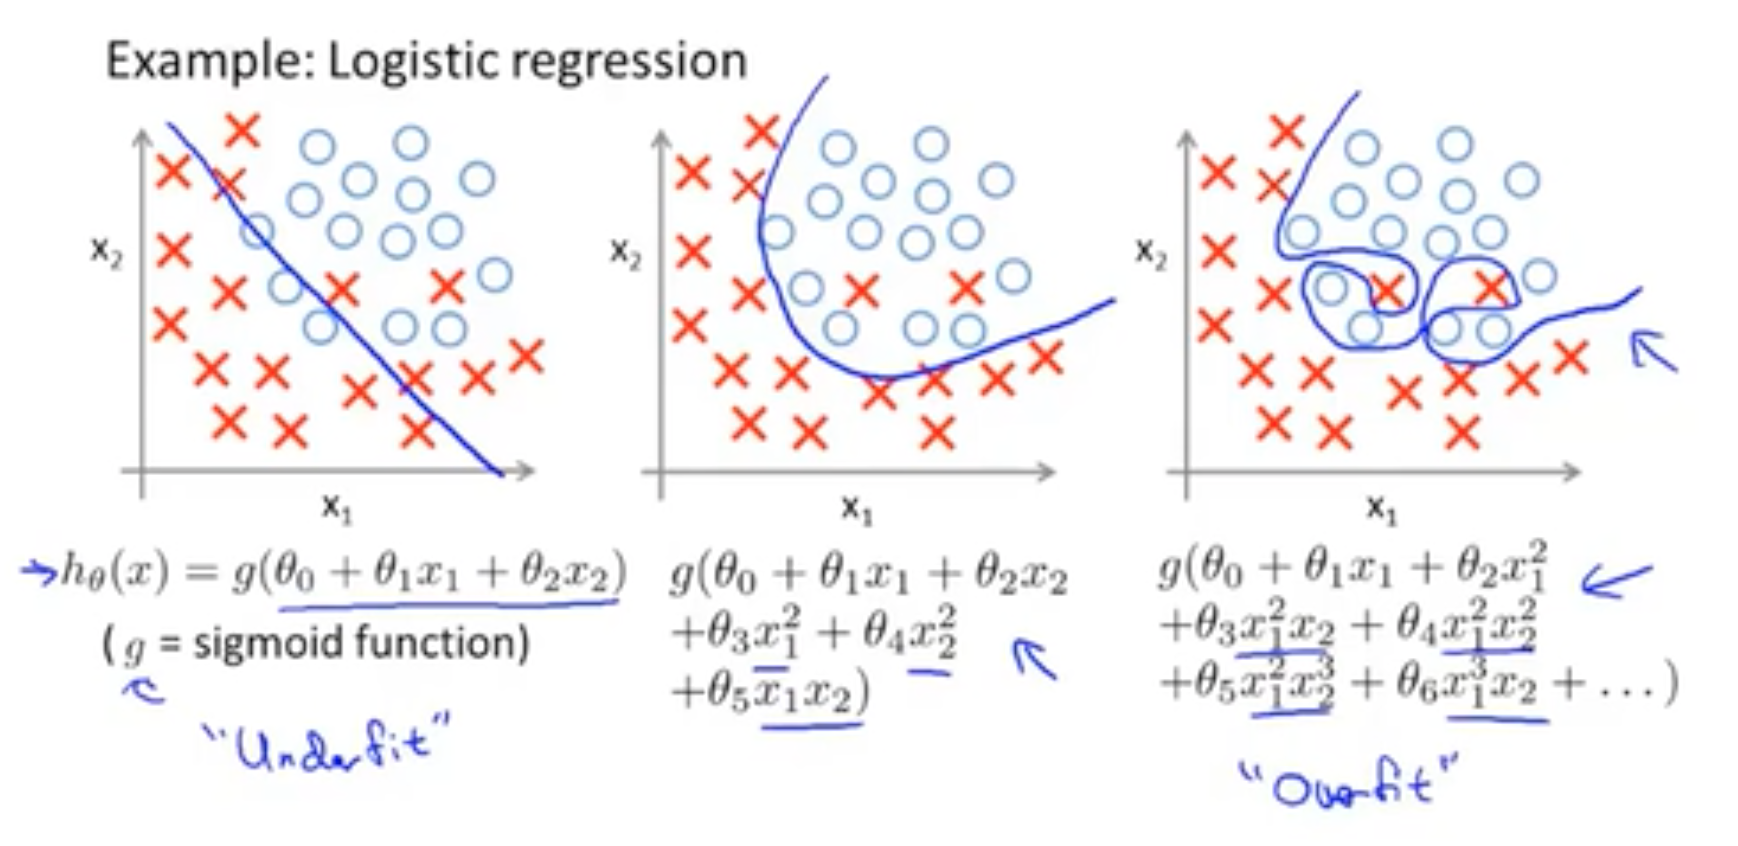
\includegraphics[width=0.8\linewidth]{figs/Chap_5_img2.png}
\end{figure}

解决过拟合的方法有很多，这里学习正则化方法（Regularization）。


\subsection{正则化}

仍然以多项式回归为例，如果我们的假设函数为：$h_\theta(x)=\theta_0+\theta_1x+\theta_2x^2+\theta_3x^3+\theta_4x^4$，而其中的高阶项 $\theta_3,\theta_4$ 导致了过拟合问题，那么我们自然希望 $\theta_3$ 和 $\theta_4$ 越小越好。此时，我们只需要对代价函数做出一点修改：$J(\theta)=\frac{1}{2m}\left[\sum\limits_{i=1}^m\left(h_\theta(x^{(i)})-y^{(i)}\right)^2+1000\theta_3^2+1000\theta_4^2\right]$，这样当 $J(\theta)$ 取最小时，$\theta_3$ 和 $\theta_4$ 都接近于 $0$，我们也就达到了目的。

一般地，我们并不知道究竟应该对哪些参数做出“惩罚”，所以我们设代价函数为：
\[
J(\theta)=\frac{1}{m}\sum_{i=1}^m\text{Cost}\left(h_\theta(x^{(i)})-y^{(i)}\right)+\frac{\lambda}{2m}\sum_{j=1}^n\theta_j^2
\]
其中，$\lambda$ 是正则化参数，$\lambda\sum\limits_{j=1}^n\theta_j^2$ 是正则化项。即我们对\textbf{除了 $\theta_0$ 以外}的参数都做“惩罚”。

如何理解这个代价函数呢？使前一项 $\frac{1}{m}\sum\limits_{i=1}^m\text{Cost}\left(h_\theta(x^{(i)})-y^{(i)}\right)$ 尽可能小是为了去拟合数据集中的数据，使正则化项 $\frac{\lambda}{2m}\sum\limits_{j=1}^n\theta_j^2$ 尽可能小是为了减小各 $\theta_j$ 以避免过拟合，而 $\lambda$ 就是在二者之间权衡的参数。如果 $\lambda$ 很大，意味着正则化项占主要地位，有可能导致所有的 $\theta_j$ 都太小了而无法拟合好数据，即欠拟合；如果 $\lambda$ 很小，意味着拟合数据占主要地位，就有可能过拟合。所以一个合适的正则化参数 $\lambda$ 非常重要。


\paragraph{线性回归的正则化}

线性回归的含有正则化项的代价函数为：
\begin{align*}
J(\theta)&=\frac{1}{2m}\left[\sum_{i=1}^m\left(h_\theta(x^{(i)})-y^{(i)}\right)^2+\lambda\sum_{j=1}^n\theta_j^2\right]\\
&=\frac{1}{2m}\left[\sum_{i=1}^m\left(\theta^Tx^{(i)}-y^{(i)}\right)^2+\lambda\sum_{j=1}^n\theta_j^2\right]
\end{align*}
对其求导：
\[
\frac{\partial J}{\partial \theta_j}=\frac{1}{m}\sum_{i=1}^m\left(\theta^Tx^{(i)}-y^{(i)}\right)x^{(i)}_j+[j\neq 0]\frac{\lambda}{m}\theta_j,\quad j=0,1,\cdots,n
\]
所以梯度下降时，我们的迭代过程为：
\begin{align*}
\theta_j&:=\theta_j-\alpha \frac{\partial J}{\partial \theta_j}\\
&=\theta_j-\alpha \left[\frac{1}{m}\sum_{i=1}^m\left(\theta^Tx^{(i)}-y^{(i)}\right)x^{(i)}_j+\frac{\lambda}{m}\theta_j\right]\\
&=\theta_j\left(1-\alpha\frac{\lambda}{m}\right)-\alpha\frac{1}{m}\sum_{i=1}^m\left(\theta^Tx^{(i)}-y^{(i)}\right)x^{(i)}_j,\quad j=1,\cdots,n
\end{align*}

若不用梯度下降，而是直接用正规方程，即在数学上解它，那么：

为了记号的方便，我们先假定对 $\theta_0$ 也进行“惩罚”。首先将 $J(\theta)$ 写作矩阵形式：
\begin{align*}
J(\theta)&=\frac{1}{2m}\left[\sum_{i=1}^m\left(\theta^Tx^{(i)}\right)^2-2\sum_{i=1}^m\theta^Tx^{(i)}y^{(i)}+\sum_{i=1}^m\left(y^{(i)}\right)^2+\lambda\theta^T\theta\right]\\
&=\frac{1}{2m}\left[\left(\theta^TX^T\right)\left(\theta^TX^T\right)^T-2\theta^TX^Ty+y^Ty+\lambda\theta^T\theta\right]\\
&=\frac{1}{2m}\left[\theta^TX^TX\theta-2\theta^TX^Ty+y^Ty+\lambda\theta^T\theta\right]
\end{align*}
然后令
\[
\frac{\partial J}{\partial \theta}=\frac{1}{m}\left[X^TX\theta-X^Ty+\lambda\theta\right]=0
\]
则：
\[
(X^TX+\lambda)\theta=X^Ty
\]
解得：
\[
\theta=(X^TX+\lambda)^{-1}X^Ty
\]
现在把 $j=0$ 的特殊情况考虑进去，那么最后的结果就是：
\[
\theta=\left(X^TX+\lambda\begin{bmatrix}0&&&\\&1&&\\&&\ddots&\\&&&1\end{bmatrix}\right)^{-1}X^Ty
\]


\paragraph{逻辑回归的正则化}

逻辑回归的含有正则化项的代价函数为：
\begin{align*}
J(\theta)&=-\frac{1}{m}\sum_{i=1}^m\left[y^{(i)}\ln(h_\theta(x^{(i)}))+(1-y^{(i)})\ln(1-h_\theta(x^{(i)}))\right]+\frac{\lambda}{2m}\sum_{j=1}^n\theta_j^2\\
&=\frac{1}{m}\sum_{i=1}^m\left[y^{(i)}\ln\left(1+e^{-\theta^Tx^{(i)}}\right)+\left(1-y^{(i)}\right)\ln\left(1+e^{\theta^Tx^{(i)}}\right)\right]+\frac{\lambda}{2m}\sum_{j=1}^n\theta_j^2
\end{align*}
对其求导：
\[
\frac{\partial J}{\partial \theta_j}=\frac{1}{m}\sum_{i=1}^m\left(h_\theta(x^{(i)})-y^{(i)}\right)x^{(i)}_j+[j\neq 0]\frac{\lambda}{m}\theta_j,\quad j=0,1,\cdots,n
\]
所以梯度下降时，我们的迭代过程为：
\begin{align*}
\theta_0&:=\theta_0-\alpha\frac{\partial J}{\partial\theta_j}\\
&=\theta_0-\alpha\frac{1}{m}\sum_{i=1}^m\left(h_\theta(x^{(i)})-y^{(i)}\right)x_0^{(i)}
\\
\theta_j&:=\theta_j-\alpha \frac{\partial J}{\partial \theta_j}\\
&=\theta_j-\alpha \left[\frac{1}{m}\sum_{i=1}^m\left(h_\theta(x^{(i)})-y^{(i)}\right)x^{(i)}_j+\frac{\lambda}{m}\theta_j\right]\\
&=\theta_j\left(1-\alpha\frac{\lambda}{m}\right)-\alpha\frac{1}{m}\sum_{i=1}^m\left(h_\theta(x^{(i)})-y^{(i)}\right)x^{(i)}_j,\quad j=1,\cdots,n
\end{align*}

和线性回归一样，我们更希望将上面的式子写作矩阵形式。

注意：以下表达式与 \texttt{numpy} 的矩阵形式相对应，即存在 "broadcast" 的表示方式，在数学上不一定严谨。



\paragraph{代价函数的矩阵形式}

回顾逻辑回归的代价函数：
\[
J(\theta)=\frac{1}{m}\sum_{i=1}^m\left[-y^{(i)}\ln(h_\theta(x^{(i)}))-(1-y^{(i)})\ln(1-h_\theta(x^{(i)}))\right]
\]
其中，
\[
h_\theta(x)=g(\theta^Tx)=\frac{1}{1+e^{-\theta^Tx}}
\]
设：
\[
X=\begin{bmatrix}(x^{(1)})^T\\(x^{(2)})^T\\\vdots\\(x^{(m)})^T\end{bmatrix}\quad \theta=\begin{bmatrix}\theta_0\\\theta_1\\\vdots\\\theta_n\end{bmatrix}\quad y=\begin{bmatrix}y^{(0)}\\y^{(1)}\\\vdots\\y^{(m)}\end{bmatrix}
\]
于是：
\[
X\theta=\begin{bmatrix}(x^{(1)})^T\theta\\(x^{(2)})^T\theta\\\vdots\\(x^{(m)})^T\theta\end{bmatrix}=\begin{bmatrix}\theta^T(x^{(1)})\\\theta^T(x^{(2)})\\\vdots\\\theta^T(x^{(m)})\end{bmatrix}
\]
所以，设：
\[
h'_\theta(X)=1/(1+e^{-X\theta})\in\mathbb R^{m}
\]
于是：
\[
J(\theta)=-\frac{1}{m}\left[y^T\ln(h'_\theta(X))+(1-y^T)\ln(1-h'_\theta(X))\right]
\]


\paragraph{代价函数偏导的矩阵形式}

逻辑回归的代价函数的偏导函数向量：
\[
\frac{\partial J}{\partial \theta}=\frac{1}{m}\sum_{i=1}^m\left[\left(h_\theta(x^{(i)})-y^{(i)}\right)x^{(i)}\right]=\frac{1}{m}X^T(h'_\theta(X)-y)
\]


\paragraph{正则化后的矩阵形式}

回顾正则化后的逻辑回归代价函数及其偏导：
\begin{align*}
J(\theta)&=\frac{1}{m}\sum_{i=1}^m\left[-y^{(i)}\ln(h_\theta(x^{(i)}))-(1-y^{(i)})\ln(1-h_\theta(x^{(i)}))\right]+\frac{\lambda}{2m}\sum_{j=1}^n\theta_j^2\\
\frac{\partial J}{\partial \theta}&=\frac{1}{m}\sum_{i=1}^m\left(h_\theta(x^{(i)})-y^{(i)}\right)x^{(i)}+\frac{\lambda}{m}\hat\theta
\end{align*}
注意，这里 $\hat\theta=\begin{bmatrix}0\\\theta_1\\\vdots\\\theta_n\end{bmatrix}$，即在 $\theta$ 中将 $\theta_0$ 换成 $0$. 

有了之前的推导，就容易写出正则化后的矩阵形式了：
\begin{align*}
J(\theta)&=-\frac{1}{m}\left[y^T\ln(h'_\theta(X))+(1-y^T)\ln(1-h'_\theta(X))\right]+\frac{\lambda}{2m}\hat\theta^T\hat\theta\\
\frac{\partial J}{\partial \theta}&=\frac{1}{m}X^T(h'_\theta(X)-y)+\frac{\lambda}{m}\hat\theta
\end{align*}
这也是我们使用 `numpy` 实现正则化逻辑回归时的表达式。


\subsection{代码实现}

首先还是来看一下数据集：

\begin{figure}[H]
    \centering
    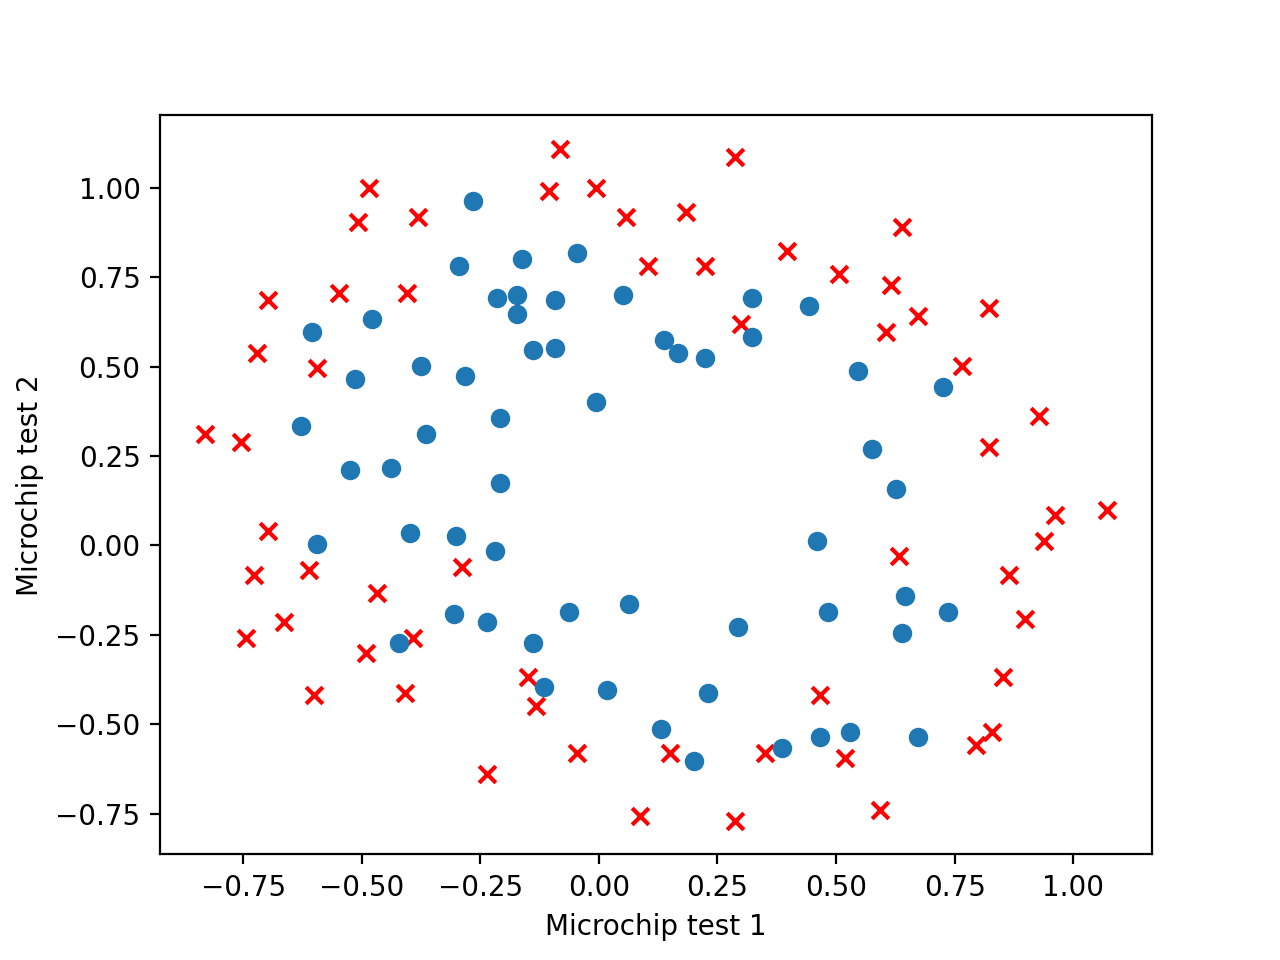
\includegraphics[width=0.5\linewidth]{figs/Chap_5_Figure_0.png}
\end{figure}

显然，我们需要用一个多项式去进行逻辑回归，这里将数据的两维都扩充为 $3$ 次，形成有 $16$ 维特征的数据，然后进行逻辑回归。

\begin{lstlisting}[language=Python]
import numpy as np
import matplotlib.pyplot as plt

alpha = 0.01
lamb = 1
iteration = 1000000
Z = []

def h(Theta, x):
	return 1 / (1 + np.exp(-np.matmul(Theta.T, x)[0][0]))

def h_(Theta, X):
	return 1 / (1 + np.exp(-np.matmul(X, Theta)))

def J_reg(Theta, X, y):
	tmp = h_(Theta, X)
	return (-(np.matmul(y.T, np.log(tmp)) + np.matmul(1 - y.T, np.log(1 - tmp))) / m\
		 + lamb / 2 / m * np.matmul(Theta.T, Theta))[0][0]

def partJ_reg(Theta, X, y):
	return (np.matmul(X.T, h_(Theta, X) - y) + lamb * np.vstack((np.zeros((1, 1)), Theta[1:, :]))) / m

def GradientDescent(X, Y):
	T = np.zeros((n, 1))
	for t in range(iteration):
		T = T - alpha * partJ_reg(T, X, Y)
		Z.append(J_reg(T, X, Y))
	return T

def extend(x1, x2):
	X = []
	for j in range(4):
		for k in range(4):
			X.append(np.power(x1, j) * np.power(x2, k))
	return X

data = np.genfromtxt("ex2data2.txt", delimiter = ',')
(m, n) = data.shape
Y = data[:, -1:]
n = 16
X = np.zeros((m, n))
for i in range(m):
	X[i] = extend(data[i][0], data[i][1])

T = GradientDescent(X, Y)
print(T.T)
print(J_reg(T, X, Y))

#============================== draw the picture ==============================#

def calc(x1, x2):
	res = np.zeros((x1.shape[0], x1.shape[1]))
	for ix in range(x1.shape[0]):
		for iy in range(x1.shape[1]):
			tmp = np.array(extend(x1[ix][iy], x2[ix][iy]), ndmin = 2)
			res[ix][iy] = h(T, tmp.T)
	return res

minx1, maxx1 = data[:, 0].min(), data[:, 0].max()+0.1
minx2, maxx2 = data[:, 1].min(), data[:, 1].max()+0.1
delta = 0.01
x1, x2 = np.meshgrid(np.arange(minx1, maxx1, delta), np.arange(minx2, maxx2, delta))

p1 = plt.subplot(121)
plt.contour(x1, x2, calc(x1, x2), [0.5], colors = 'magenta')

X0 = data[data[:, -1] == 0, :]
X1 = data[data[:, -1] == 1, :]
p1.set_title("lambda = " + str(lamb))
p1.set_xlabel("Microchip test 1")
p1.set_ylabel("Microchip test 2")
p1.scatter(X0[:, 0:1], X0[:, 1:2], marker = 'x', c = 'r')
p1.scatter(X1[:, 0:1], X1[:, 1:2], marker = 'o')

p2 = plt.subplot(122)
p2.plot(range(1, iteration+1), Z)
p2.set_title("lambda = " + str(lamb))
p2.set_xlabel("Iteration")
p2.set_ylabel("Cost")

plt.show()
\end{lstlisting}

以下是 $\lambda=0,1,5$ 的回归结果和收敛情况：

\begin{figure}[H]
    \centering
    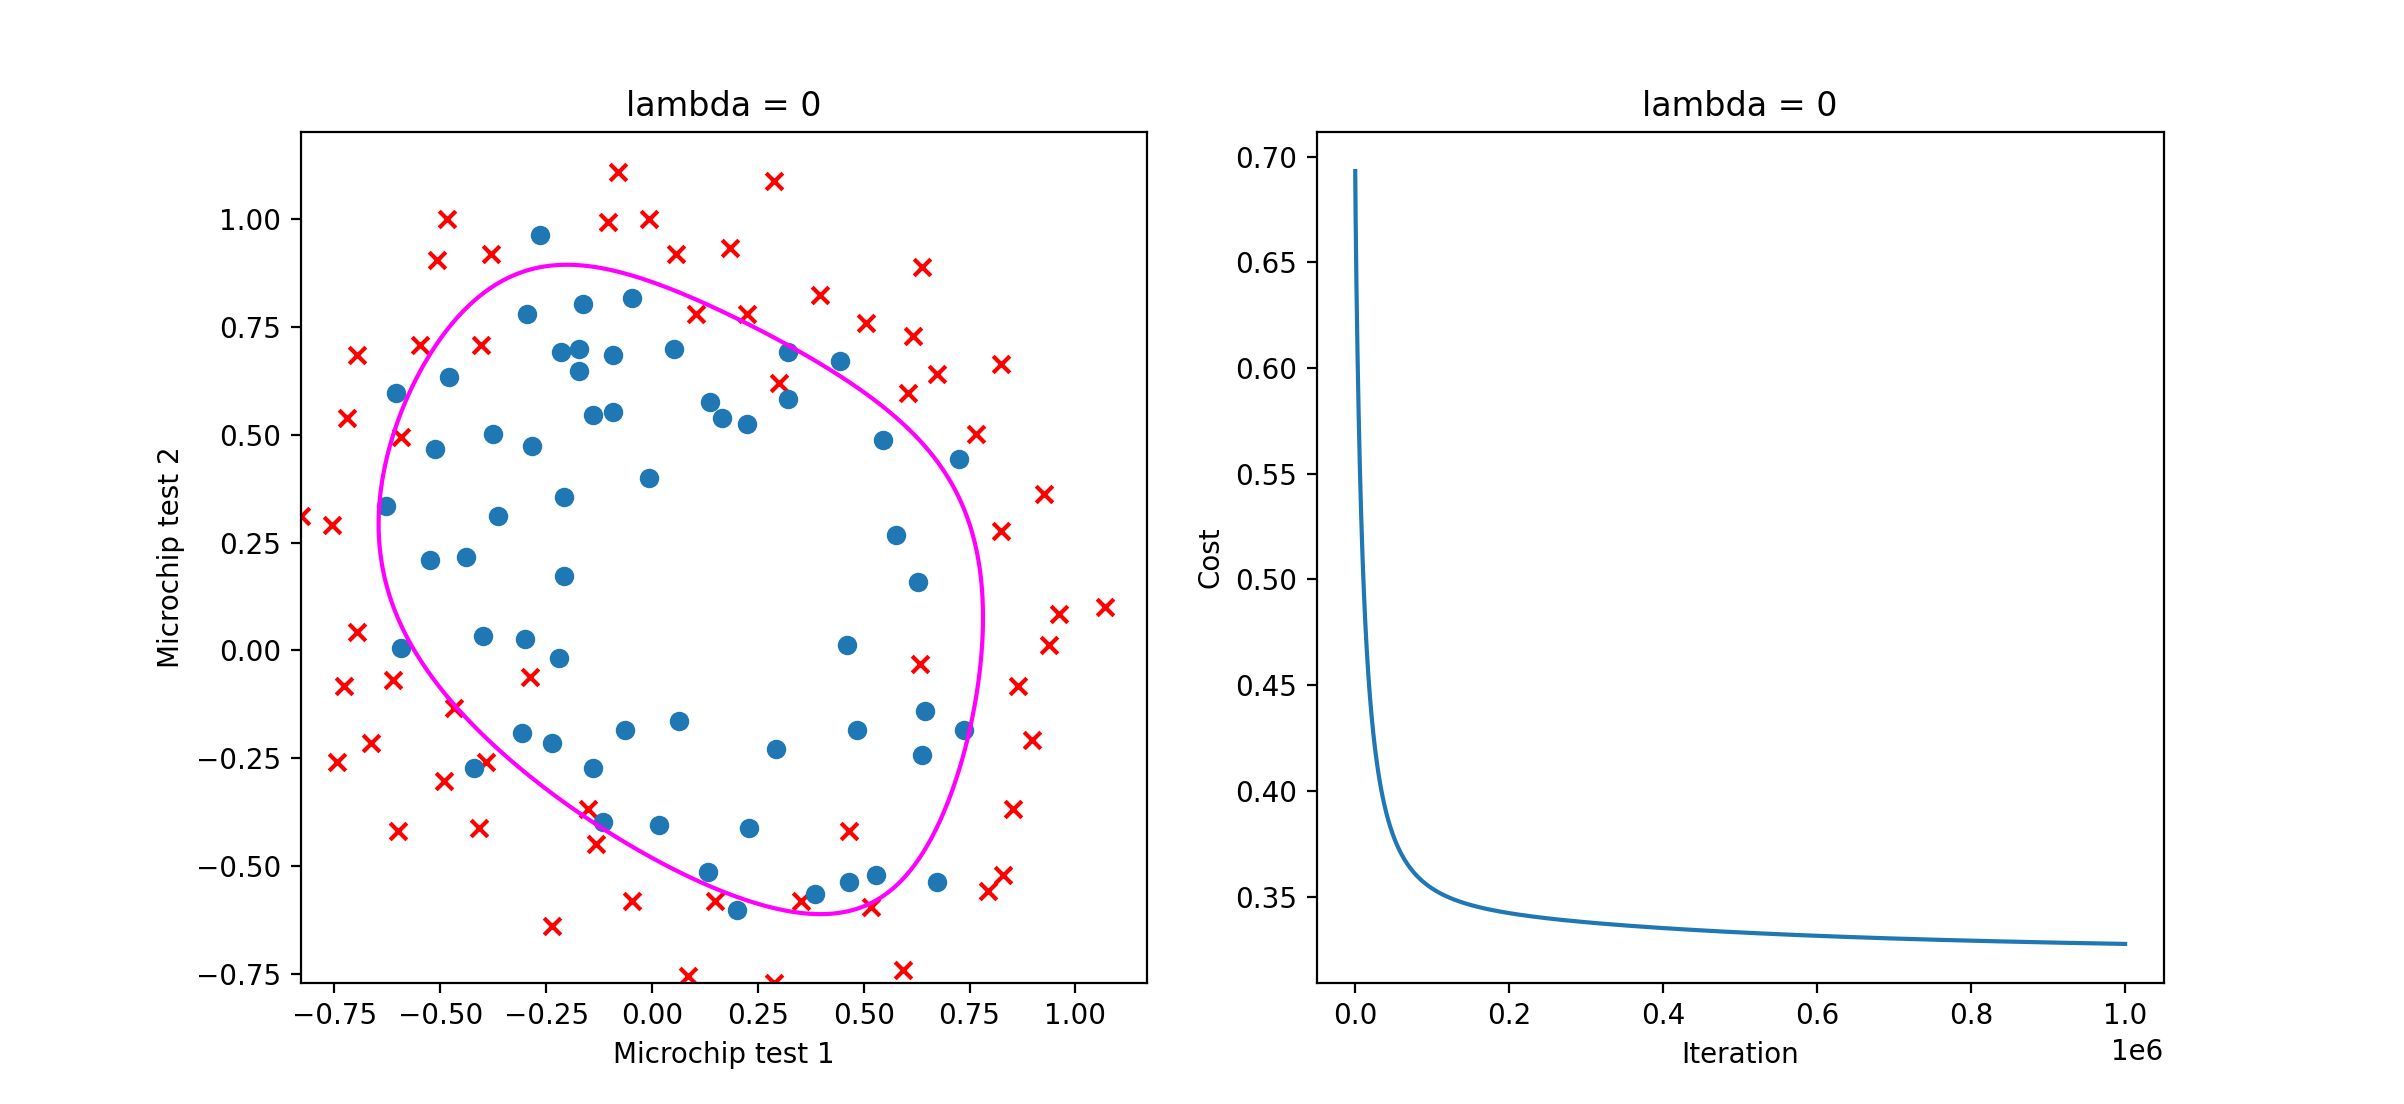
\includegraphics[width=\linewidth]{figs/Chap_5_Figure_11.png}
\end{figure}

\begin{figure}[H]
    \centering
    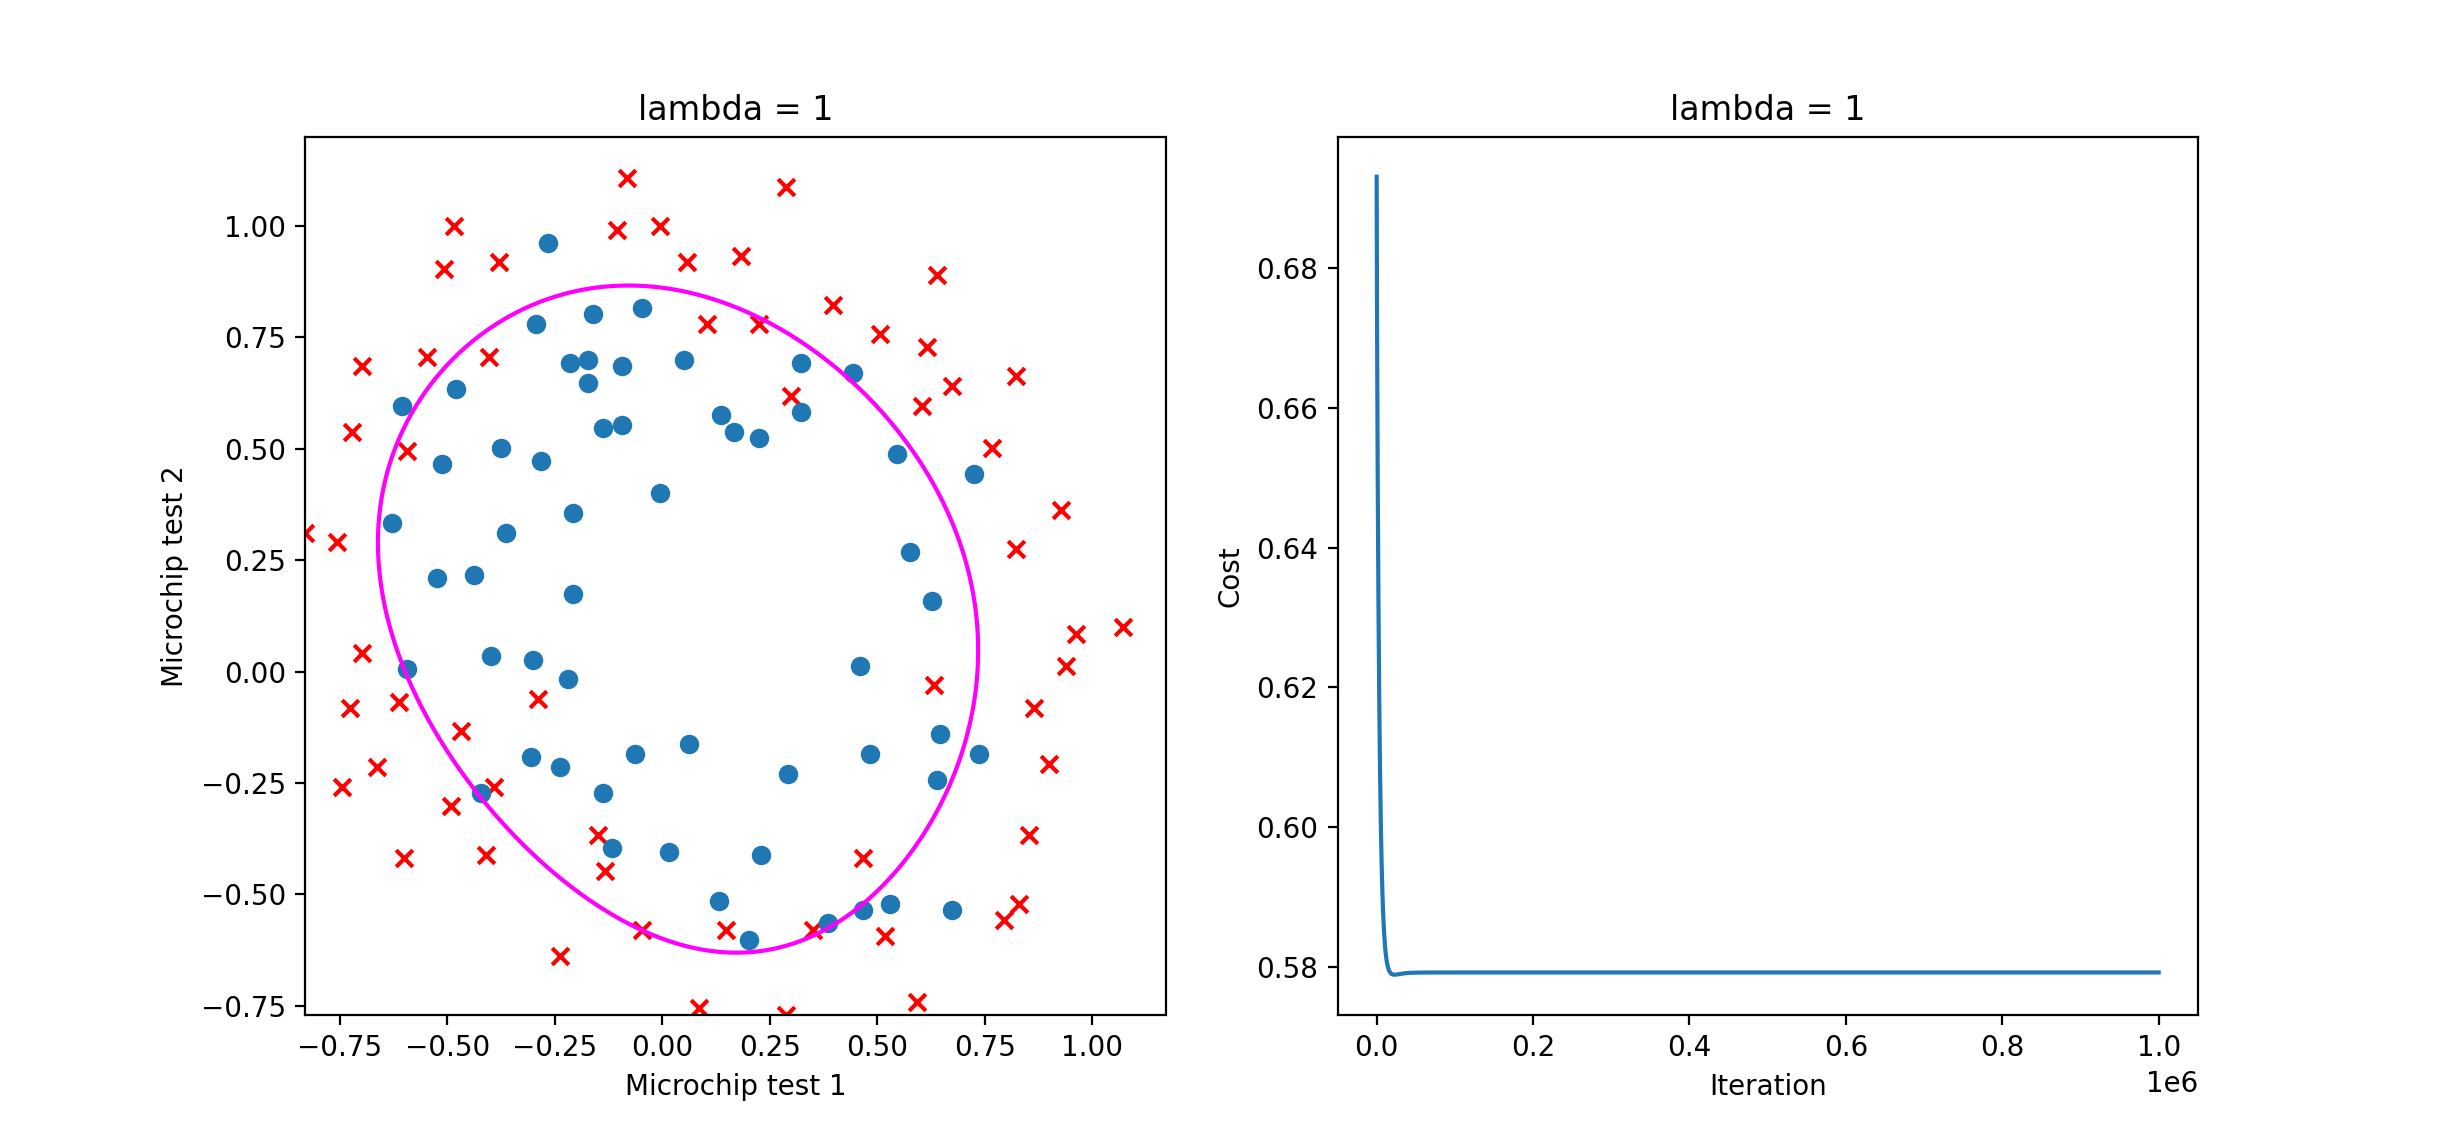
\includegraphics[width=\linewidth]{figs/Chap_5_Figure_12.png}
\end{figure}

\begin{figure}[H]
    \centering
    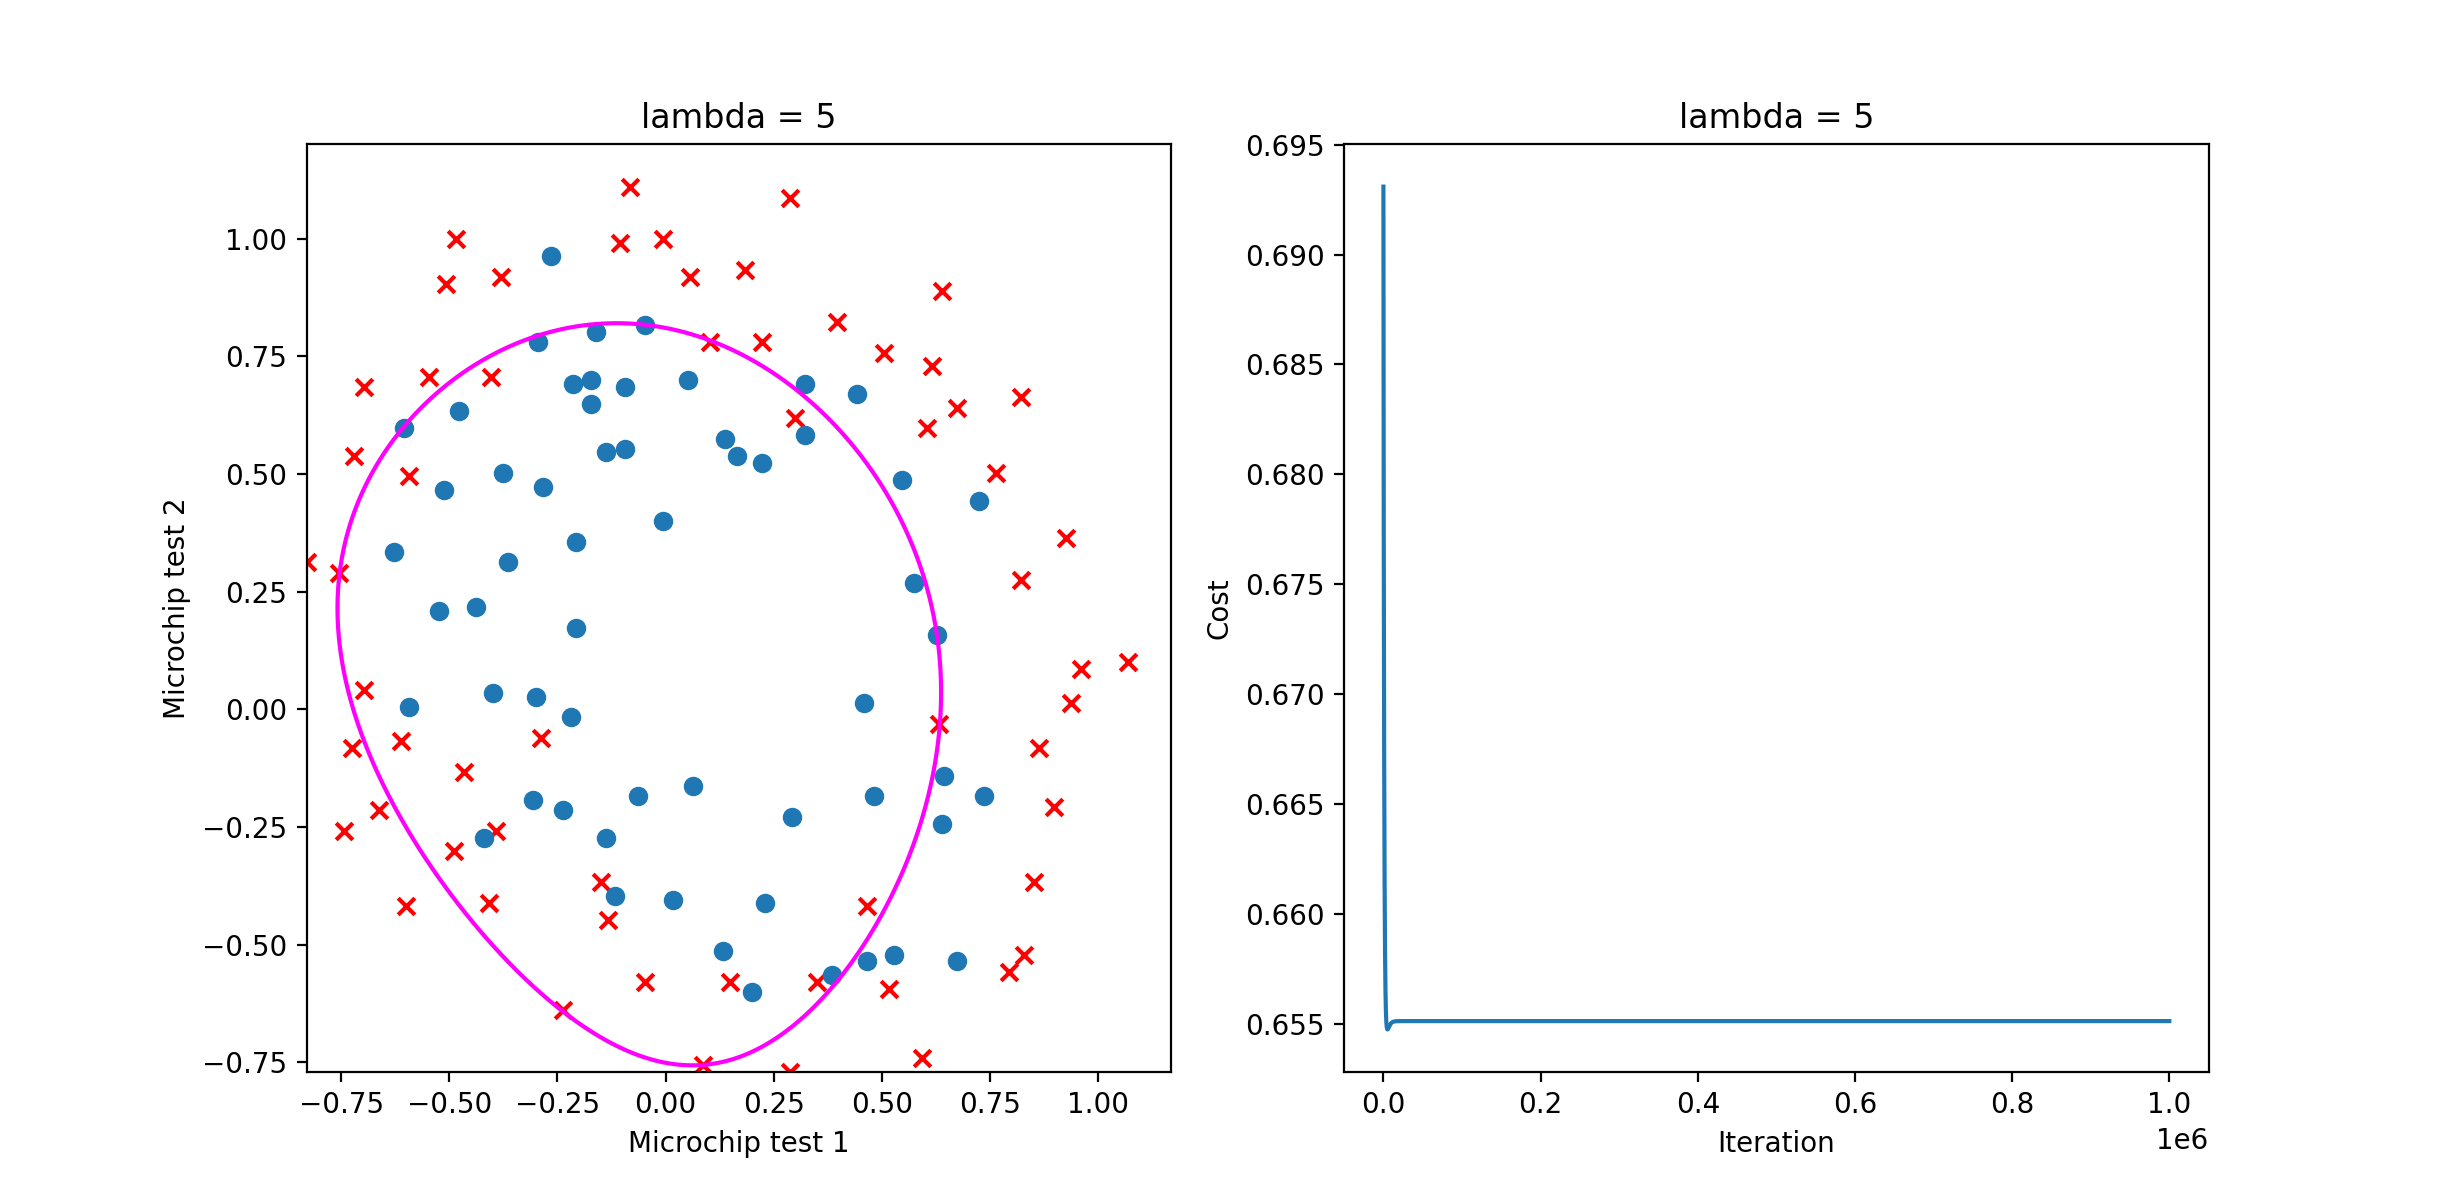
\includegraphics[width=\linewidth]{figs/Chap_5_Figure_13.png}
\end{figure}


接下来我换了一个生成特征的方式：

\begin{lstlisting}[language=Python]
def extend(x1, x2):
	X = []
	for j in range(6 + 1):
		for k in range(j + 1):
			X.append(np.power(x1, k) * np.power(x2, j-k))
	return X
\end{lstlisting}

结果如下：

\begin{figure}[H]
    \centering
    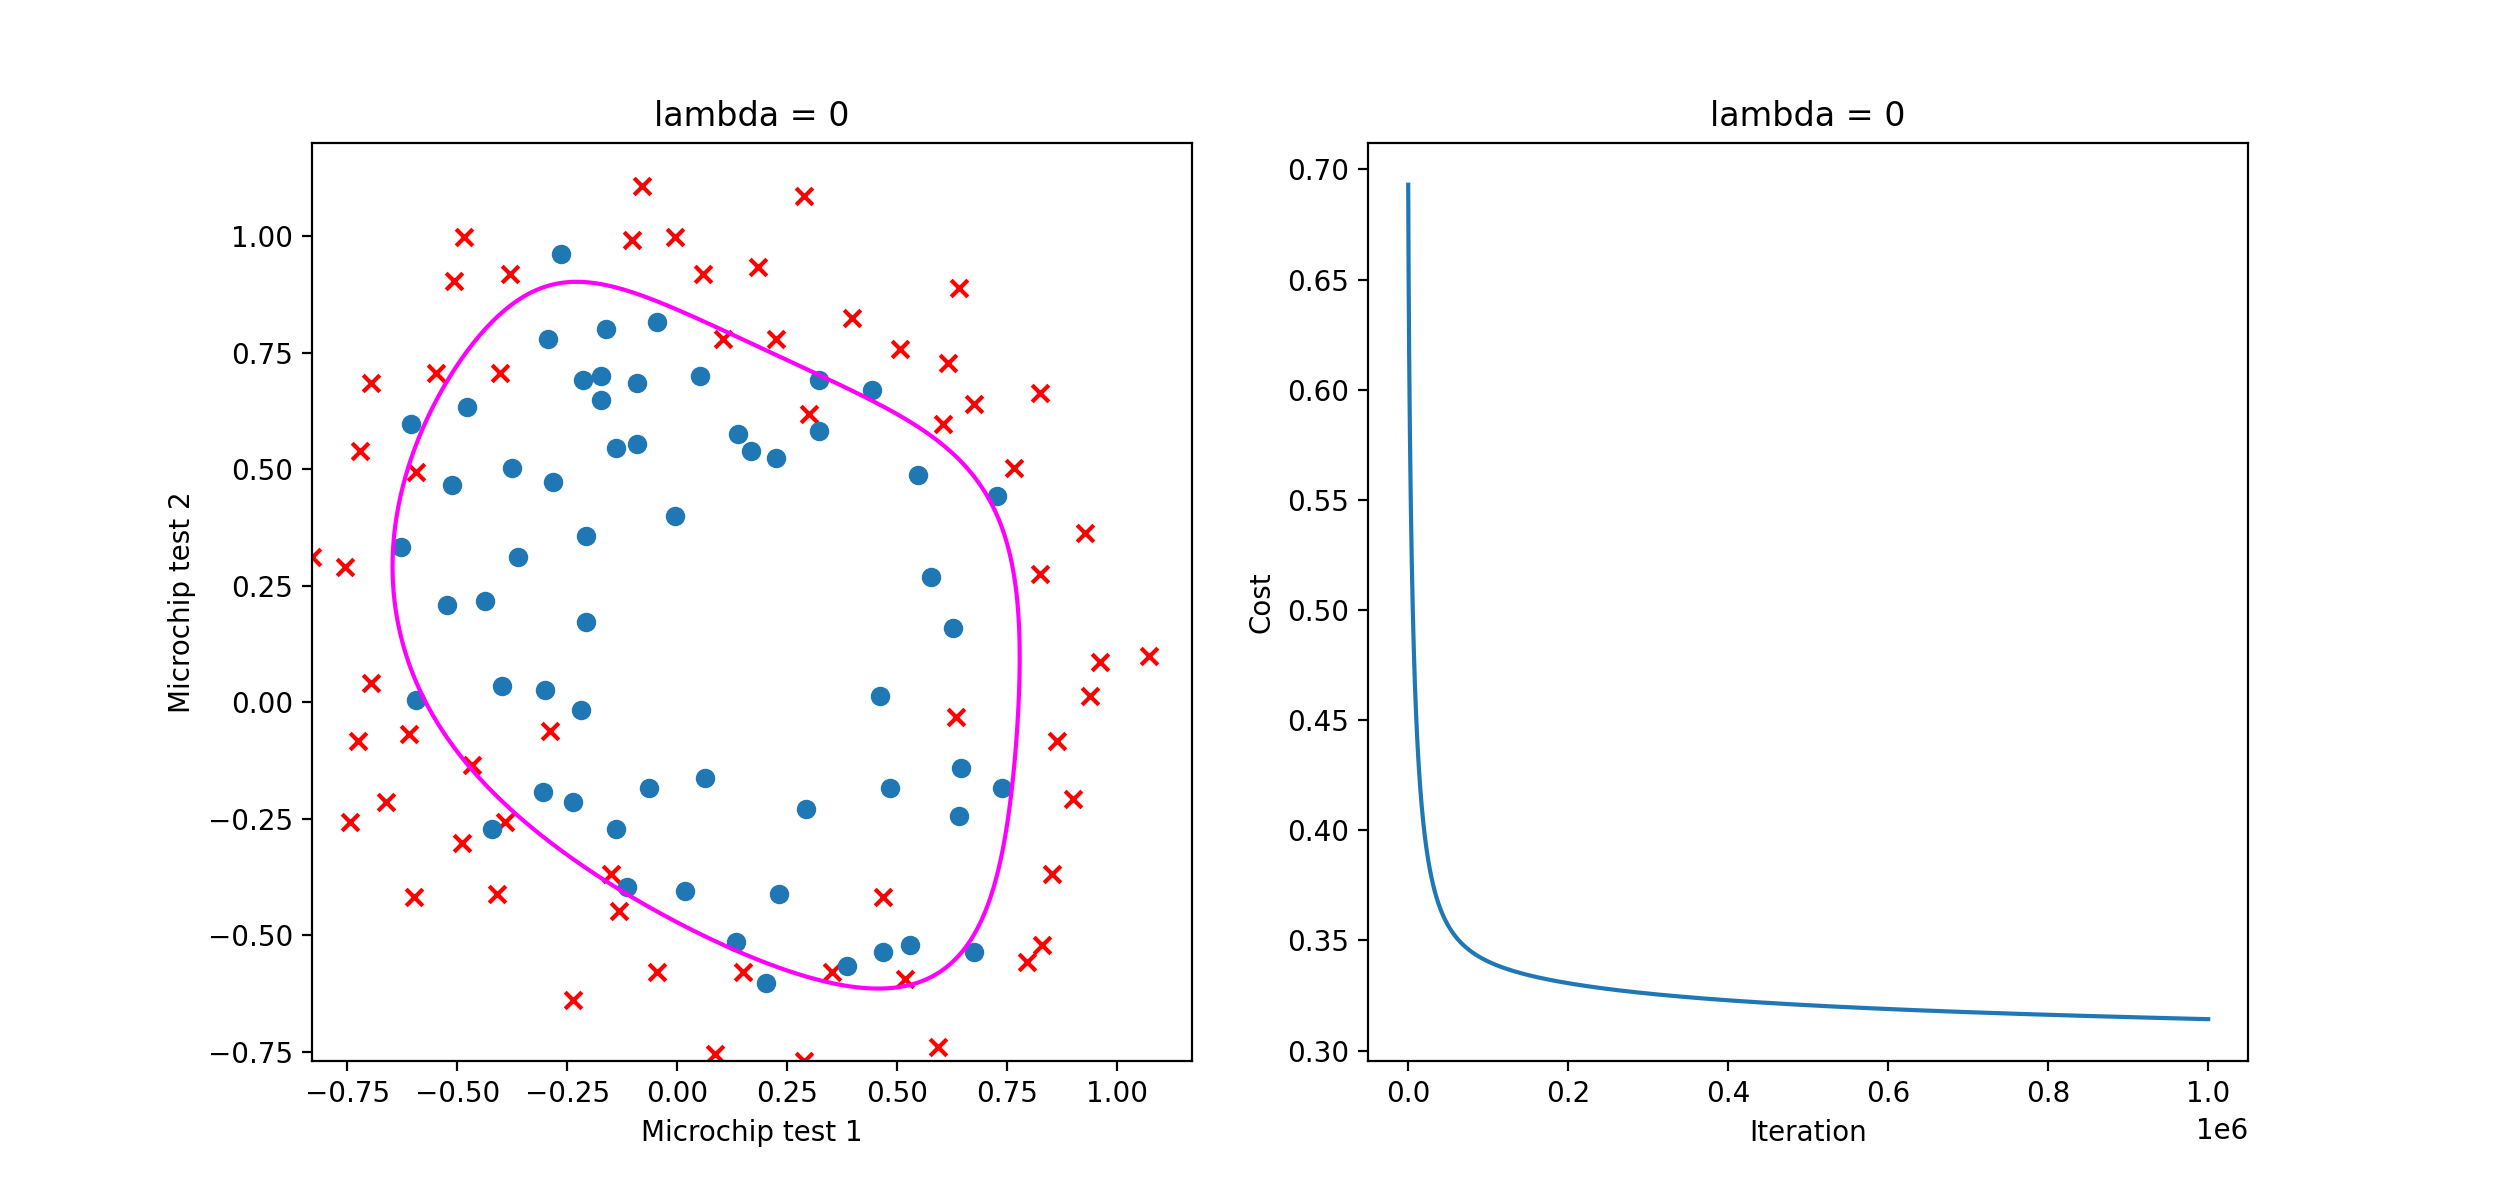
\includegraphics[width=\linewidth]{figs/Chap_5_Figure_21.png}
\end{figure}

\begin{figure}[H]
    \centering
    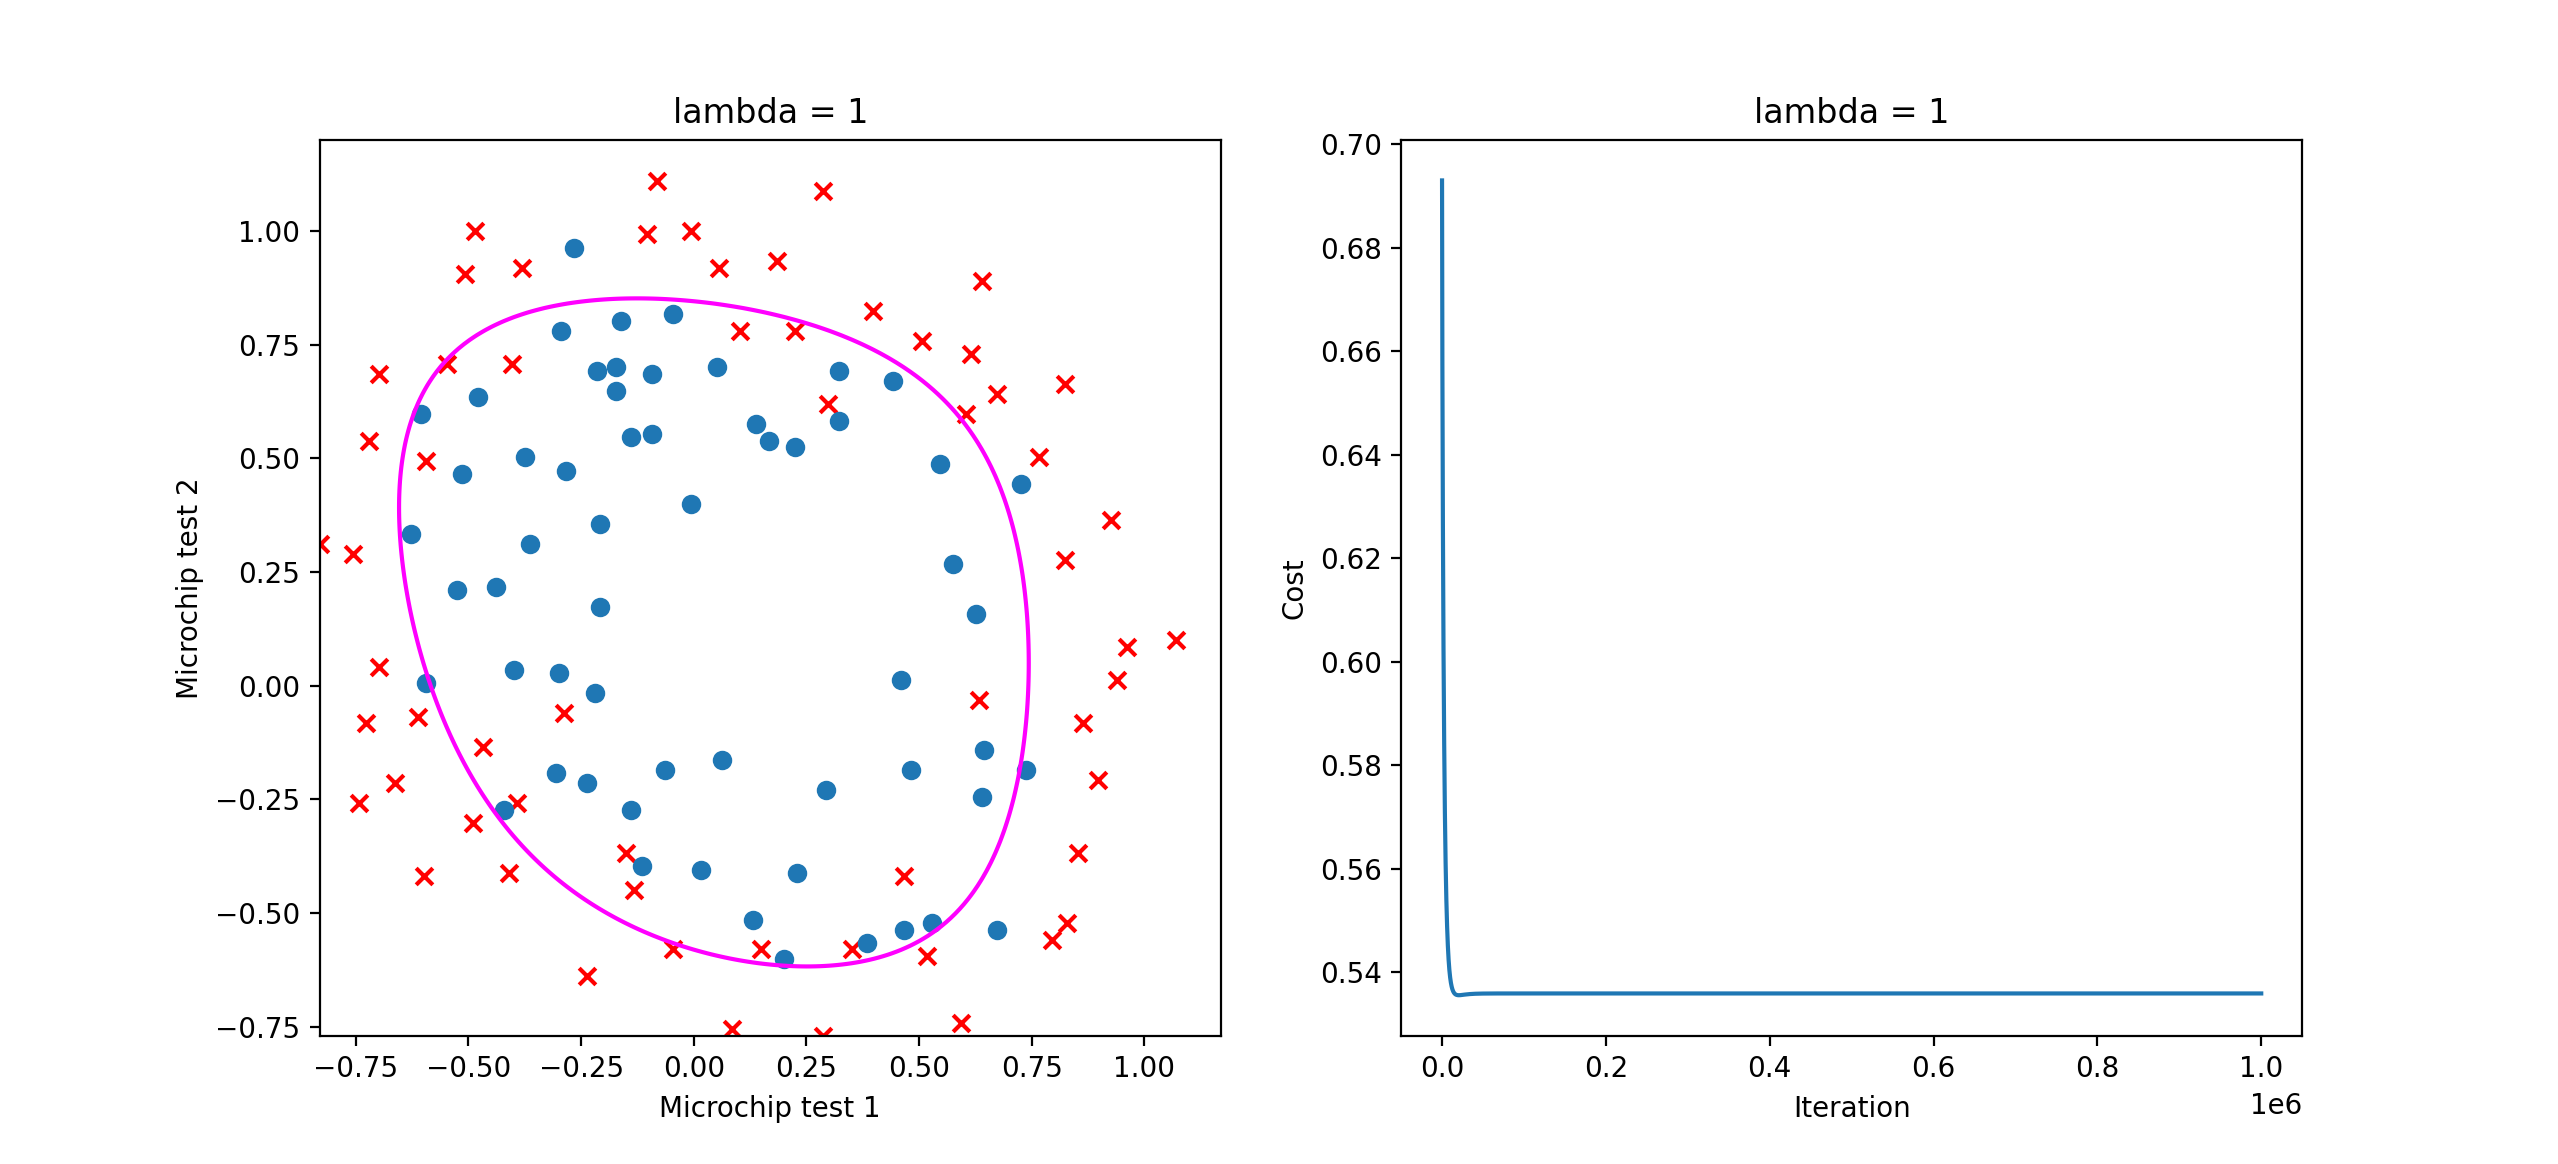
\includegraphics[width=\linewidth]{figs/Chap_5_Figure_22.png}
\end{figure}

\begin{figure}[H]
    \centering
    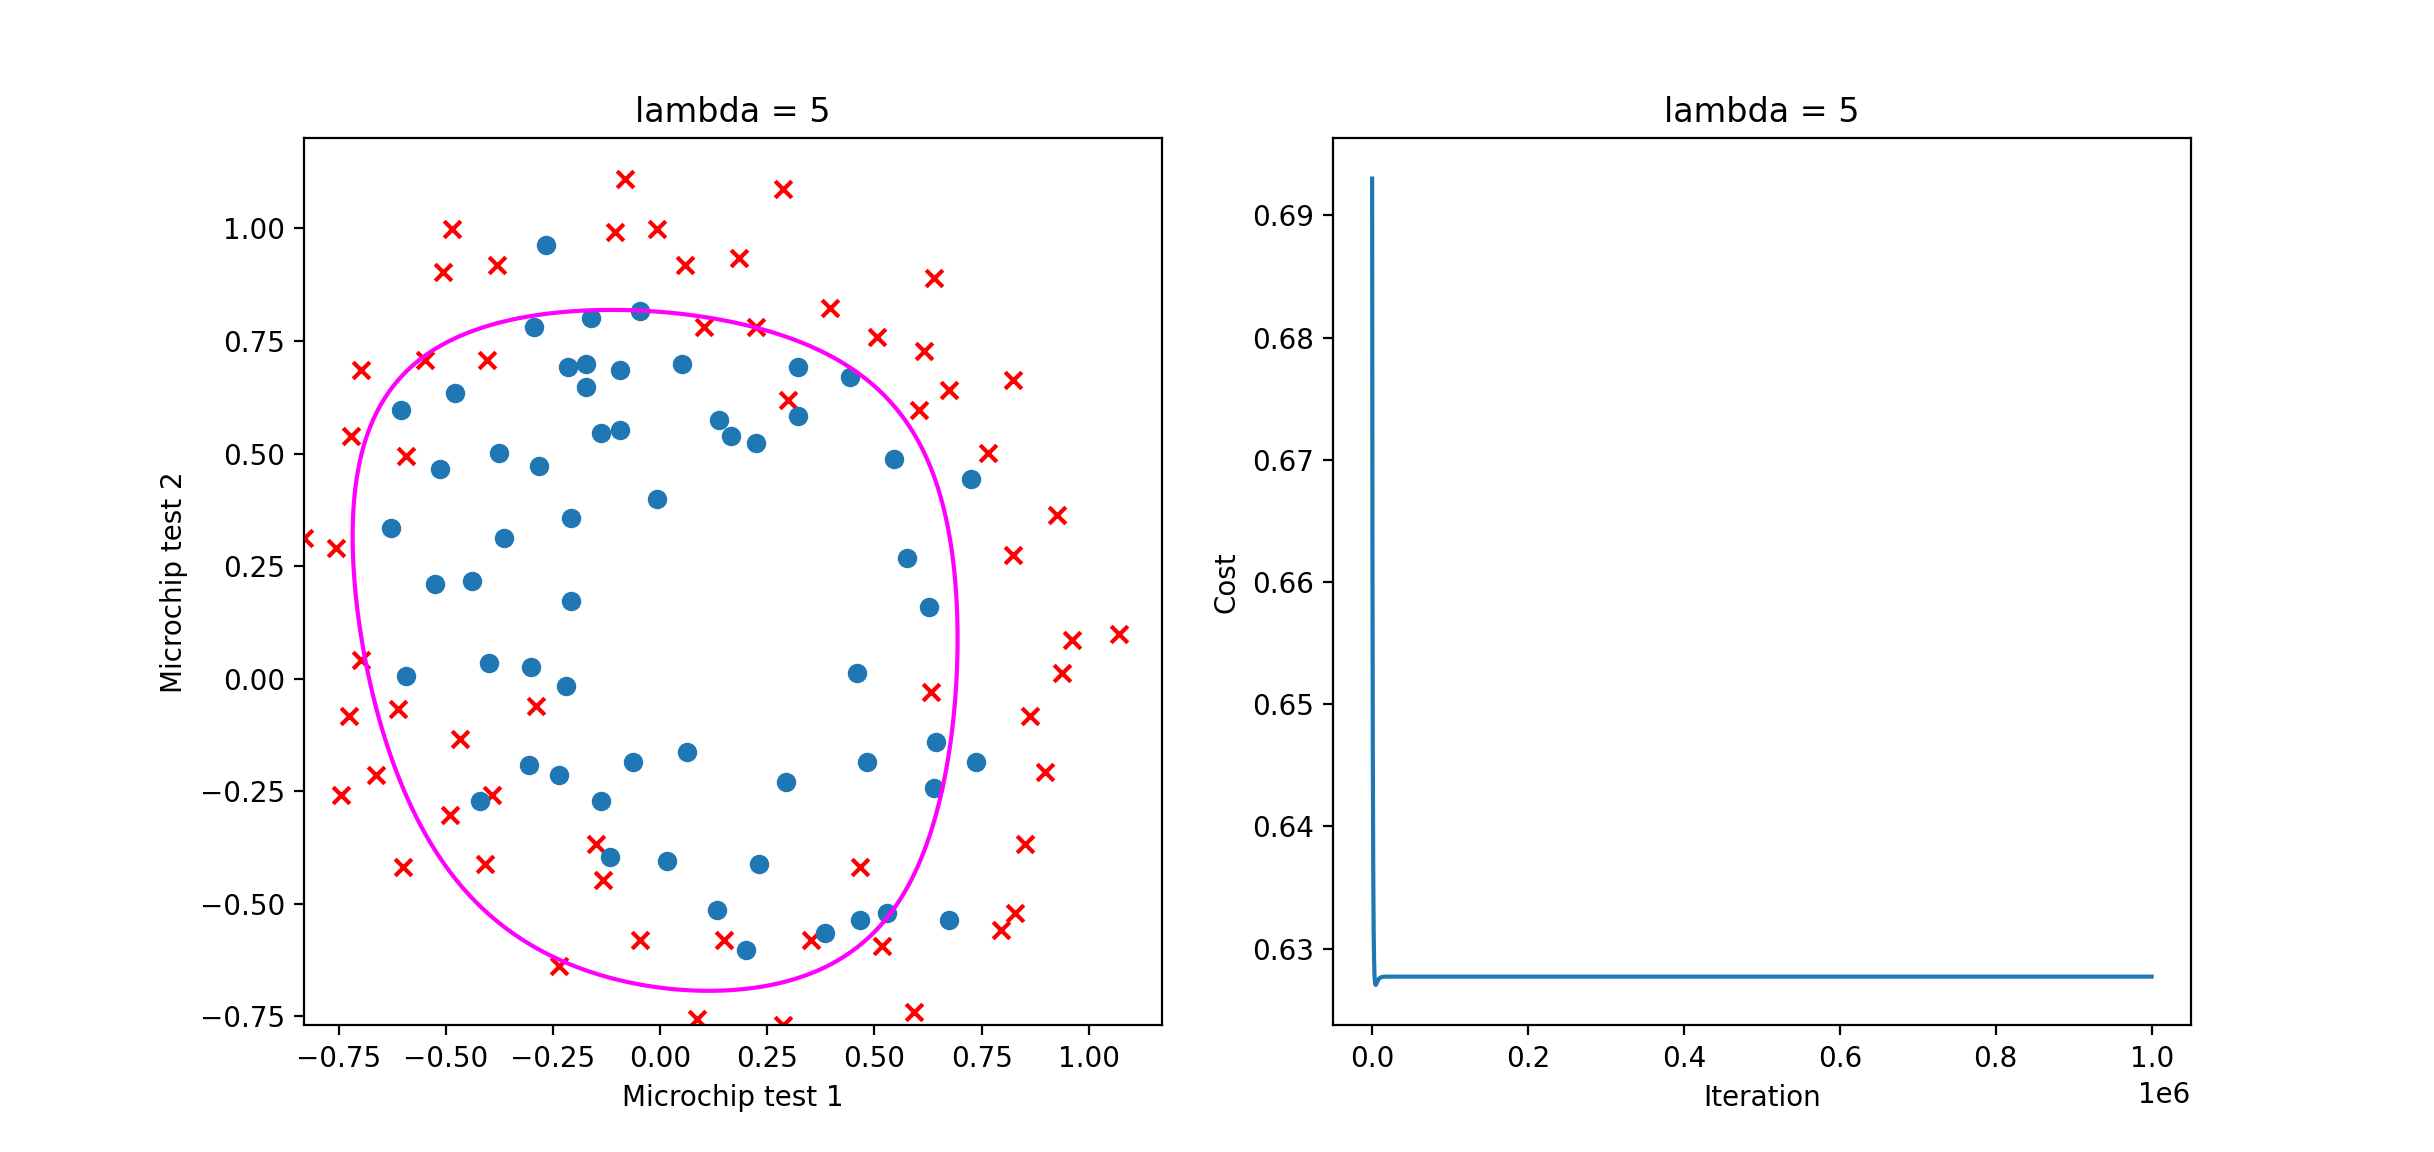
\includegraphics[width=\linewidth]{figs/Chap_5_Figure_23.png}
\end{figure}
 \newpage
\section{逻辑回归之多分类（数字识别）}
\label{sec:chapter6}

\subsection{数据读入与显示}

数据采用 \texttt{.mat} 格式，可以使用 \texttt{scipy} 中的 \texttt{loadmat} 方法读取：

\begin{lstlisting}[language=Python]
import numpy as np
from scipy.io import loadmat

data = loadmat('ex3data1.mat')
print(data)
print(data['X'].shape)
print(data['y'].shape)
```

```
{'__header__': b'MATLAB 5.0 MAT-file, Platform: GLNXA64, Created on: Sun Oct 16 13:09:09 2011', '__version__': '1.0', '__globals__': [], 'X': array([[0., 0., 0., ..., 0., 0., 0.],
       [0., 0., 0., ..., 0., 0., 0.],
       [0., 0., 0., ..., 0., 0., 0.],
       ...,
       [0., 0., 0., ..., 0., 0., 0.],
       [0., 0., 0., ..., 0., 0., 0.],
       [0., 0., 0., ..., 0., 0., 0.]]), 'y': array([[10],
       [10],
       [10],
       ...,
       [ 9],
       [ 9],
       [ 9]], dtype=uint8)}
(5000, 400)
(5000, 1)
\end{lstlisting}

文件中共有 $5000$ 个样本。每个样本的输入是由 $20\times 20$ 灰度图像展开得到的 $400$ 维向量，输出为图像对应的数字标签。

\begin{note}
由于 \texttt{MATLAB} 或 \texttt{Octave} 的数据约定，数字 $0$ 被标记为 $10$，使用 \texttt{Python} 时可以将其恢复为 $0$. 此外，图像数据按列展开，还原为 $20\times20$ 矩阵后需要转置。
\end{note}

\begin{lstlisting}[language=Python]
data = loadmat('ex3data1.mat')
X = data['X']
X = np.transpose(X.reshape((5000, 20, 20)), [0, 2, 1]).reshape(5000, 400)
y = data['y']
y[y==10] = 0
\end{lstlisting}

随机选取 $100$ 幅图像，显示结果如下：

\begin{lstlisting}[language=Python]
def show_a_number(num, ax):
	"""
	num.shape: (400, )
	"""
	ax.matshow(num.reshape((20, 20)), cmap=matplotlib.cm.binary)
	ax.axis('off')

fig, ax = plt.subplots(10, 10)
for i in range(10):
	for j in range(10):
		id = np.random.randint(0, 5000)
		show_a_number(X[id, :], ax[i][j])
plt.show()
\end{lstlisting}

\begin{figure}[H]
    \centering
    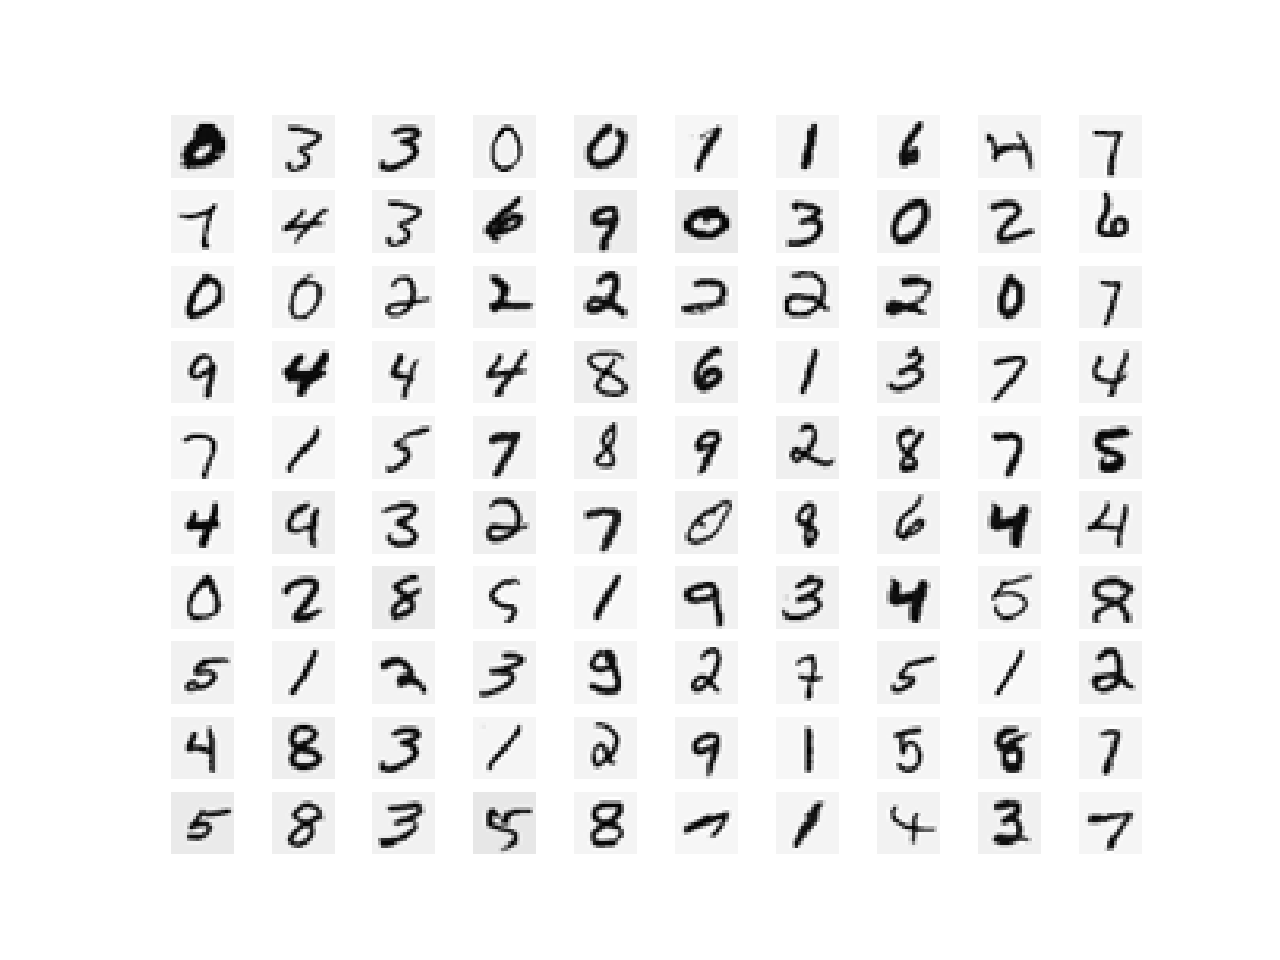
\includegraphics[width=0.6\linewidth]{figs/Chap_6_Figure_0.png}
\end{figure}


\subsection{多分类}

这里采用“一对多”策略完成多分类。对于每一个数字，都单独训练一个逻辑回归分类器：属于当前数字的样本标记为正类，其余数字全部标记为负类。这样便可将一个十分类问题转化为 $10$ 个二分类问题。预测时，分别计算所有分类器给出的概率，并选择概率最大的类别作为最终结果。

沿用上一节的矩阵化正则逻辑回归代码，分别训练 $10$ 个分类器。注意需要在 $X$ 的每一行前添加一个 $1$ 作为偏置项。

\begin{lstlisting}[language=Python]
import numpy as np
from scipy.io import loadmat
import matplotlib.pyplot as plt
import matplotlib

lamb = 1
alpha = 0.1
iteration = 10000
m = 5000
n = 401

data = loadmat('ex3data1.mat')
X = data['X']
X = np.transpose(X.reshape((m, 20, 20)), [0, 2, 1]).reshape(m, 400)
X = np.hstack((np.ones((m, 1)), X))
y = data['y']
y[y==10] = 0

def h(Theta, x):
	return 1 / (1 + np.exp(-np.matmul(Theta.T, x)[0][0]))

def h_(Theta, X):
	return 1 / (1 + np.exp(-np.matmul(X, Theta)))

def J_reg(Theta, X, y):
	tmp = h_(Theta, X)
	return (-(np.matmul(y.T, np.log(tmp)) + np.matmul(1 - y.T, np.log(1 - tmp))) / m\
		 + lamb / 2 / m * np.matmul(Theta.T, Theta))[0][0]

def partJ_reg(Theta, X, y):
	return (np.matmul(X.T, h_(Theta, X) - y) + lamb * np.vstack((np.zeros((1, 1)), Theta[1:, :]))) / m

def GradientDescent(X, y):
	Theta = np.zeros((n, 1))
	for t in range(iteration):
		Theta = Theta - alpha * partJ_reg(Theta, X, y)
	return Theta

def classify(k):
	y_ = y.copy()
	y_[y==k] = 1
	y_[y!=k] = 0
	Theta = GradientDescent(X, y_)
	return Theta

Theta = np.zeros((10, n))
for k in range(10):
	Theta[k, :] = classify(k).flatten()
	print("Trained for:", k)

np.savetxt('theta.txt', Theta, delimiter=',')
\end{lstlisting}

训练得到的参数保存至 \texttt{theta.txt}. 预测时读入该矩阵，对同一个输入同时计算 $10$ 个分类器的输出，再取最大值对应的数字：

\begin{lstlisting}[language=Python]
def predict(Theta, x):
	return np.matmul(Theta, x).argmax(axis=0)
\end{lstlisting}

训练集上各数字的准确率如下。注意：训练集准确率并不能作为模型评估结果，详见第 \ref{sec:chapter9} 章。

\begin{table}[H]
    \centering
    \small
    \begin{tabularx}{\linewidth}{lYYYYYYYYYYY}
    \toprule
    数字 & 0 & 1 & 2 & 3 & 4 & 5 & 6 & 7 & 8 & 9 & Total \\
    \midrule
    准确率 & 99.0\% & 97.8\% & 88.2\% & 90.0\% & 93.4\% & 89.4\% & 97.0\% & 93.8\% & 91.4\% & 91.2\% & 93.1\% \\
    \bottomrule
    \end{tabularx}
\end{table}
 \newpage
\section{初识神经网络}
\label{sec:chapter7}

\subsection{神经元模型}

\begin{figure}[H]
    \centering
    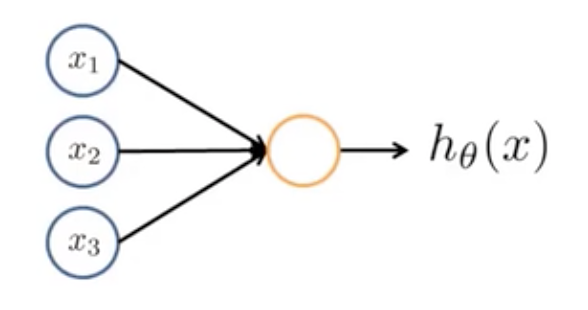
\includegraphics[width=0.4\linewidth]{figs/Chap_7_neuron.png}
    \vspace{-2ex}
\end{figure}

神经元可以视为一个函数：它接收上一层节点的输出，将各输入按权重组合，再经过激活函数得到新的输出，即：
\[
h_\theta(x)=f(\theta, x)
\]
这里 $\theta=(\theta_0,\theta_1,\cdots,\theta_n)^T,\,x=(x_0,x_1,\cdots,x_n)^T$.

\begin{note}
上图省略了 $x_0\equiv 1$ 这一偏置项。
\end{note}

神经元输出 $h_\theta(x)$ 由激活函数计算。激活函数为神经网络引入非线性，使多层网络能够表示比单纯线性变换更复杂的关系。此处采用 $\text{sigmoid}$ 函数，即 $h_\theta(x)=g(\theta^Tx)=\frac{1}{1+e^{-\theta^Tx}}$. 


\subsection{神经网络}

\begin{figure}[H]
    \centering
    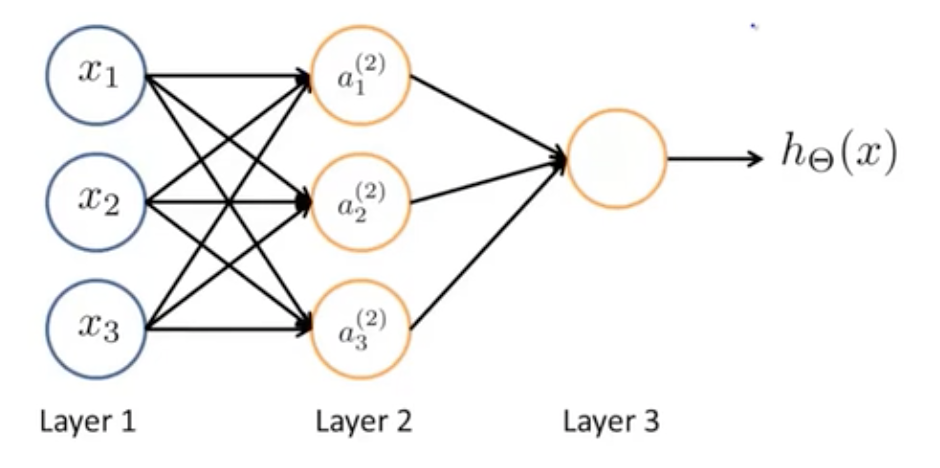
\includegraphics[width=0.5\linewidth]{figs/Chap_7_neuron_network.png}
    \vspace{-2ex}
\end{figure}

神经网络由多层相互连接的神经元组成。第一层称为输入层，负责接收原始特征；最后一层称为输出层，给出模型的预测；位于二者之间的各层称为隐藏层。信息从输入层开始，逐层计算并传递到输出层，这一过程称为前向传播。

\begin{note}
上图同样省略了 $x_0(a_0^{(1)})\equiv a_0^{(2)}\equiv1$ 偏置项。
\end{note}

下面单独分析第 $i$ 层到第 $i+1$ 层的传播过程。设 $s_i$ 为第 $i$ 层的神经元数量（\textbf{不包含偏置项}），则第 $i+1$ 层的每个神经元都与一组独立参数对应。对于第 $k$ 个神经元，其参数记为 $\theta^{(i)}_k$，并满足 $a^{(i+1)}_k=h_{\theta^{(i)}_k}(\hat a^{(i)})=g\left({\theta_k^{(i)}}^T\hat a^{(i)}\right)$. 其中，$\hat a^{(i)}\in\mathbb R^{s_i+1}$ 表示在 $a^{(i)}$ 前加入偏置项后的向量。将下一层所有神经元的计算合并，即可写成矩阵形式：
\[
a^{(i+1)}=g\left(\Theta^{(i)}\hat a^{(i)}\right)
\]
其中，$\Theta^{(i)}\in\mathbb R^{s_{i+1}\times(s_i+1)}$. 

\begin{note}
也可以将偏置项对应的参数向量 $b$ 单独列出，将上式写为：
\[
a^{(i+1)}=g\left(\Theta^{(i)}a^{(i)}+b^{(i)}\right)
\]
其中，$\Theta^{(i)}\in\mathbb R^{s_{i+1}\times s_i},\,b\in\mathbb R^{s_{i+1}}$. 本文仍沿用前一种写法。
\end{note}


\subsection{神经网络实现门电路}

下面通过门电路示例直观说明神经网络参数如何控制输出。

考虑一个输入层有 $2$ 个神经元（不包括偏置项）且取值 $\in\{0,1\}$、输出层有 $1$ 个神经元且取值 $\in\{0,1\}$ 的神经网络。如果我们将其参数设置为：$\Theta^{(1)}=(-30,20,20)^T$，那么我们有：

\begin{table}[H]
    \centering
    \begin{tabularx}{0.4\linewidth}{cYc}
      \toprule
      输入 1 & 输入 2 & 输出 \\
      \midrule
      0 & 0 & $g(-30)\approx 0$ \\
      0 & 1 & $g(-10)\approx 0$ \\
      1 & 0 & $g(-10)\approx 0$ \\
      1 & 1 & $g(10)\approx 1$  \\
      \bottomrule
    \end{tabularx}
\end{table}

从表中可以看出，只有两个输入同时为 $1$ 时，线性组合才为正且输出接近 $1$；其他情况下输出均接近 $0$. 因此，这个神经元实现了与门。

通过选择不同参数，同样可以实现或门和非门。进一步将这些基本门组合起来，多层神经网络还可以表示单个线性分类器无法直接实现的异或门、同或门等逻辑电路。这也说明隐藏层能够逐层组合较简单的特征，形成更复杂的决策规则。


\subsection{代码实现}

本节仍以手写数字识别为例，但暂不训练参数。参数 $\Theta$ 已在 \texttt{ex3weights.mat} 中给出，只需按照神经网络结构逐层执行前向传播。

\begin{lstlisting}[language=Python]
import numpy as np
from scipy.io import loadmat
import matplotlib.pyplot as plt
import matplotlib

m = 5000
n = 401

data = loadmat('ex3data1.mat')
X = data['X'] # (5000, 400)
X = np.hstack((np.ones((m, 1)), X)) # (5000, 401)
y = data['y'] # (5000, 1)

data = loadmat('ex3weights.mat')
Theta1 = data['Theta1'] # (25, 401)
Theta2 = data['Theta2'] # (10, 26)

def sigmoid(z):
	return 1 / (1 + np.exp(-z))

def predict(x):
	"""
	x: (401, )
	"""
	a1 = x.reshape((401, 1))
	a2 = np.matmul(Theta1, a1)
	a2 = sigmoid(a2) # (25, 1)
	a2 = np.vstack((np.ones((1, 1)), a2)) # (26, 1)
	a3 = np.matmul(Theta2, a2)
	a3 = sigmoid(a3)
	return a3.argmax(axis=0)[0] + 1

Sum = np.zeros(11)
Hit = np.zeros(11)
Accuracy = np.zeros(11)
hit = 0
for id in range(5000):
	Sum[y[id][0]] += 1
	if predict(X[id, :].T) == y[id][0]:
		Hit[y[id][0]] += 1
		hit += 1
for i in range(1, 11):
	Accuracy[i] = Hit[i] / Sum[i]
	print(str(i)+":", str(Accuracy[i] * 100)+"%")
print("tot:", str(hit / 5000 * 100)+"%")
\end{lstlisting}

各数字及整体的准确率如下：

\begin{table}[H]
    \centering
    \small
    \begin{tabularx}{\linewidth}{lYYYYYYYYYYY}
    \toprule
    数字 & 1 & 2 & 3 & 4 & 5 & 6 & 7 & 8 & 9 & 0 & Total \\
    \midrule
    准确率 & 98.2\% & 97.0\% & 96.0\% & 96.8\% & 98.4\% & 98.6\% & 97.0\% & 98.2\% & 95.8\% & 99.2\% & 97.5\% \\
    \bottomrule
    \end{tabularx}
\end{table}

注意：训练集准确率并不能作为模型评估结果。
 \newpage
\section{神经网络之反向传播}
\label{sec:chapter8}

\subsection{代价函数}

回顾正则化逻辑回归的代价函数：
\[
J(\theta)=-\frac{1}{m}\left[\sum_{i=1}^my^{(i)}\ln(h_\theta(x^{(i)}))+(1-y^{(i)})\ln(1-h_\theta(x^{(i)}))\right]+\frac{\lambda}{2m}\sum_{j=1}^n\theta_j^2
\]
我们在第四篇中通过极大似然法解释了它的来历，这个代价函数被称作「交叉熵代价函数」，与我们在线性回归中使用的「二次代价函数」形成对比。

在神经网络中，我们沿用交叉熵代价函数。具体地，对于一个 $K$ 分类的神经网络而言，它可以看作是从输入到 $K$ 个二分类输出的过程：$x\mapsto h_\Theta(x)$，我们设其代价函数为每一个二分类的\textbf{交叉熵代价函数之和}：
\[
J(\Theta)=-\frac{1}{m}\left[\sum_{i=1}^m\sum_{k=1}^Ky^{(i)}_k\ln\left(h_\Theta(x^{(i)})_k\right)+(1-y_k^{(i)})\ln\left(1-h_\Theta(x^{(i)})_k\right)\right]+\frac{\lambda}{2m}\sum_{l=1}^{L-1}\sum_{i=1}^{s_l}\sum_{j=1}^{s_{l+1}}\left(\Theta_{ji}^{(l)}\right)^2
\]

其中：$h_\Theta(x^{(i)})\in\mathbb R^K$，表示从第 $i$ 个输入经由神经网络得到的输出结果，$h_\Theta(x^{(i)})_k$ 表示其第 $k$ 维. 

> 注意这里有一个符号混用的地方：上标 $^{(i)}$ 在 $x^{(i)}$ 和 $y^{(i)}$ 中表示第 $i$ 个数据的输入（$\in\mathbb R^{n+1}$）和输出（$\in\mathbb R^{K}$），但是在 $\Theta^{(l)}$ 中表示第 $l$ 层的 $\Theta$（$\in \mathbb R^{s_{l+1}\times (s_l+1)}$）. 

现在我们的目标即是最小化代价函数 $J(\Theta)$，并找到最小时的参数 $\Theta$. 

我们欲使用梯度下降法解决这个问题，所以我们需要计算 $\frac{\partial J}{\partial \Theta_{ji}^{(l)}}$，计算方法就是反向传播算法。

\subsection{反向传播算法}

\paragraph{推导}

为了推导方便，先假设只有一组数据 $(x,y)$，这样可以省去上标和求和的麻烦。我们对第 $l+1$ 层的第 $j$ 个神经元定义一个误差：
\[
\delta_j^{(l+1)}=\frac{\partial J}{\partial z_j^{(l+1)}}
\]
其中 $z_j^{(l+1)}=\sum\limits_{k=0}^{s_{l}}\Theta^{(l)}_{jk}a^{(l)}_{k}$，其实就是把对 $a_j^{(l+1)}$ 的逻辑回归单独拎出来看，取 $\text{sigmoid}$ 前的那个求和值。换句话说，$a^{(l+1)}_j=g\left(z_j^{(l+1)}\right)$. 

于是乎，我们有：
\[
\frac{\partial J}{\partial \Theta^{(l)}_{ji}}=\frac{\partial J}{\partial z_j^{(l+1)}}\cdot\frac{\partial z_j^{(l+1)}}{\partial\Theta_{ji}^{(l)}}=a_i^{(l)}\delta_j^{(l+1)}
\]
写作矩阵形式：
\[
\boxed{\Delta^{(l)}=\delta^{(l+1)}\cdot(a^{(l)})^T}
\]
所以现在问题转化为求解 $\delta^{(l+1)}$. 

采用递推的思想。首先来算输出层，即 $\delta_j^{(L)}$：
\begin{align*}
\delta_j^{(L)}&=\frac{\partial J}{\partial z_j^{(L)}}=\frac{\partial J}{\partial a_j^{(L)}}\cdot\frac{\partial a_j^{(L)}}{\partial z_j^{(L)}}\\
&=\frac{\partial J}{\partial a_j^{(L)}}\cdot g'\left(z_j^{(L)}\right)\\
&=-\left(\frac{y_j}{a_j^{(L)}}-\frac{1-y_j}{1-a_j^{(L)}}\right)\cdot\left(a_j^{(L)}(1-a_j^{(L)})\right)\\
&=a_j^{(L)}-y_j
\end{align*}

所以：
\[
\boxed{\delta^{(L)}=a^{(L)}-y}
\]

\begin{note}
上面推导过程的一些注释：

关于第二行，请注意：$a^{(L)}=g(z^{(L)})$；

关于第三行，请注意 $\text{sigmoid}$ 函数的一个很好的性质：$g'(z)=g(z)(1-g(z))$；

以及，关于偏导项的计算，请注意 $a^{(L)}=h_\Theta(x)$，所以 $J(\Theta)$ 在现在的假设条件下可以写作：
\[
J(\Theta)=-\left[\sum_{k=1}^Ky_k\ln(a^{(L)}_k)+(1-y_k)\ln(1-a_k^{(L)})\right]+\frac{\lambda}{2}\sum_{l=1}^{L-1}\sum_{i=1}^{s_l}\sum_{j=1}^{s_{l+1}}\left(\Theta_{ji}^{(l)}\right)^2
\]
\end{note}


现在计算第 $l$ 层（$2\leqslant l<L$）的 $\delta^{(l)}$：
\begin{align*}
\delta_j^{(l)}&=\frac{\partial J}{\partial z_j^{(l)}}\\
&=\frac{\partial J}{\partial z^{(l+1)}}\cdot\frac{\partial z^{(l+1)}}{\partial a_j^{(l)}}\cdot\frac{\partial a_j^{(l)}}{\partial z_j^{(l)}}\\
&={\delta^{(l+1)}}^T\Theta^{(l)}_{\bullet,j}\cdot g'(z_j^{(l)})\\
&={\delta^{(l+1)}}^T\Theta^{(l)}_{\bullet,j}\cdot \left(a_j^{(l)}*(1-a_j^{(l)})\right)
\end{align*}
所以：
\[
\boxed{\delta^{(l)}=\left({\Theta^{(l)}}^T\delta^{(l+1)}\right)*\left(a^{(l)}*(1-a^{(l)})\right)}
\]
其中 $*$ 表示两个向量对应位置相乘。


\paragraph{步骤总结}

以上是对一组数据的推导，我们得到了三个重要的结果：
\begin{align*}
&\Delta^{(l)}=\delta^{(l+1)}\cdot(a^{(l)})^T&&1\leqslant l<L\\
&\delta^{(L)}=a^{(L)}-y\\
&\delta^{(l)}=\left({\Theta^{(l)}}^T\delta^{(l+1)}\right)*\left(a^{(l)}*(1-a^{(l)})\right)&&2\leqslant l<L
\end{align*}
而 $m$ 组数据只需要在一些地方进行累加即可，具体如下：

设数据集为：$\left\{(x^{(i)},y^{(i)})\mid 1\leqslant i\leqslant m\right\}$，则反向传播算法的步骤为：

\begin{enumerate}
    \item 所有 $\Delta^{(l)}$ 置零；
    \item 遍历数据集，设当前数据为 $(x^{(i)},y^{(i)})$：
        \begin{enumerate}
            \item 以 $x^{(i)}$ 为输入做前向传播，得到输出 $a^{(L)}$；
            \item 置 $\delta^{(L)}=a^{(L)}-y^{(i)}$，进行反向传播：$\delta^{(l)}={\Theta^{(l)}}^T\delta^{(l+1)}*\left[a^{(l)}(1-a^{(l)})\right],\;2\leqslant l<L$；
            \item 更新 $\Delta$ 矩阵：$\Delta^{(l)}:=\Delta^{(l)}+\delta^{(l+1)}\cdot(a^{(l)})^T,\;1\leqslant l<L$；
        \end{enumerate}
    \item 计算 $D$ 矩阵：
       \[
       D_{ij}^{(l)}:=\begin{cases}
       \frac{1}{m}\left(\Delta_{ij}^{(l)}+\lambda\Theta_{ij}^{(l)}\right)&\text{if }j\neq0\\
       \frac{1}{m}\Delta_{ij}^{(l)}&\text{if }j=0
       \end{cases}
       \]
       这就是我们的偏导数矩阵：$\frac{\partial J}{\partial \Theta_{ij}^{(l)}}=D^{(l)}_{ij}$. 
\end{enumerate}

现在，我们可以用 $D_{ij}^{(l)}$ 做梯度下降了。注意一点，我们的参数 $\Theta^{(l)}$ 应该初始化为 $[-\epsilon,\epsilon]$ 中的随机值。


\subsection{梯度检验}

写神经网络反向传播的代码时很容易写 bug，包括一些从结果并不能发现的 bug。梯度检验可以帮助发现这些 bug。

我们可以数值近似 $J(\theta)$ 的各偏导：
\[
\frac{\partial}{\partial \theta_k}J(\theta)\approx\frac{J(\theta_1,\cdots,\theta_k+
\epsilon,\cdots,\theta_n)-J(\theta_1,\cdots,\theta_k-
\epsilon,\cdots,\theta_n)}{2\epsilon}
\]

现在我们可以比较这些偏导估计值与 $D_{ij}^{(l)}$ 对应位置的值，它们应该非常接近。

注意一点：梯度检验耗时巨大，一旦验证了神经网络反向传播的代码正确后，不应进行梯度检验（删掉/注释掉）。


\subsection{代码实现}

这次用的数据集依旧是手写数字识别的数据集，共 $5000$ 组数据，每组数据输入是一个由 $20\times20$ 灰度矩阵压缩而来的 $400$ 维向量，输出是 $0$ 到 $9$ 之间的整数。

\paragraph{第一部分·代价函数与前向传播}

前向传播与上一节的代码没有什么本质的区别，不过这里将其一般化，可适用于 $L$ 层的神经网络且 $m$ 个数据同时计算：

\begin{lstlisting}[language=Python]
def forwardPropagation():
	a = [None] * (L+1)
	a[1] = np.hstack((np.ones((m, 1)), X))
	for l in range(2, L):
		a[l] = sigmoid(np.matmul(a[l-1], Theta[l-1].T))
		a[l] = np.hstack((np.ones((m, 1)), a[l]))
	a[L] = sigmoid(np.matmul(a[L-1], Theta[L-1].T))
	return a
\end{lstlisting}

当然只计算一个数据也是可以的：

\begin{lstlisting}[language=Python]
def forwardPropagation(x):
	"""
	x: (n, 1)
	"""
	a = [None] * (L+1)
	a[1] = np.vstack((np.ones((1, 1)), x))
	for l in range(2, L):
		a[l] = sigmoid(np.matmul(Theta[l-1], a[l-1]))
		a[l] = np.vstack((np.ones((1, 1)), a[l]))
	a[L] = sigmoid(np.matmul(Theta[L-1], a[L-1]))
	return a
\end{lstlisting}

代价函数及其正则化：

\begin{lstlisting}[language=Python]
def J(lamb):
	res = 0
	FP = forwardPropagation()
	res -= np.sum(Y * np.log(FP[L]) + (1-Y) * np.log(1-FP[L]))
	for l in range(1, L):
		res += lamb / 2 * np.sum(np.power(Theta[l][:, 1:], 2))
	res /= m
	return res
\end{lstlisting}

使用 `ex4weights.mat` 中给定的参数 $\Theta$，在无正则化时，准确率为 $97.52\%$，代价为 $0.28762916516131865$；

在正则化时（$\lambda=1$），准确率为 $97.52\%$，代价为 $0.3844877962428937$。


\paragraph{第二部分·反向传播}

反向传播算法：

\begin{lstlisting}[language=Python]
def backPropagation(lamb):
	Delta = [None] * L # (s_{l+1}, s_l+1)
	for l in range(1, L):
		Delta[l] = np.zeros((s[l+1], s[l]+1))
	delta = [None] * (L+1) # (s_l, )
	a = forwardPropagation()
	for i in range(m):
		delta[L] = a[L][i:i+1, :].T - Y[i:i+1, :].T
		for l in range(L-1, 1, -1):
			delta[l] = (np.matmul(Theta[l].T, delta[l+1]) * (a[l][i:i+1, :].T * (1 - a[l][i:i+1, :].T)))[1:, :]
		for l in range(1, L):
			Delta[l] += np.matmul(delta[l+1], a[l][i:i+1, :])
	D = [None] * L # (s_{l+1}, s_l+1)
	for l in range(1, L):
		D[l] = (Delta[l] + lamb * np.hstack((np.zeros((s[l+1], 1)), Theta[l][:, 1:]))) / m
	return D
\end{lstlisting}

梯度下降：

\begin{lstlisting}[language=Python]
def GradientDescent(alpha, iteration):
	for l in range(1, L):
		Theta[l] = np.random.random((s[l+1], s[l]+1))
		Theta[l] = (Theta[l] - 0.5) / 4
	for t in range(iteration):
		D = backPropagation(lamb=1)
		for l in range(1, L):
			Theta[l] -= alpha * D[l]
		Z.append(J(lamb=1))
	return Theta
\end{lstlisting}

梯度检验（把这段代码插入到梯度下降计算出 $D$ 矩阵之后的地方即可）：

\begin{lstlisting}[language=Python]
for l in range(1, L):
    for i in range(s[l+1]):
        for j in range(s[l]+1):
            Theta[l][i, j] -= 0.001
            J1 = J(lamb=1)
            Theta[l][i, j] += 0.002
            J2 = J(lamb=1)
            Theta[l][i, j] -= 0.001
            print(D[l][i, j], (J2 - J1) / 0.002)
\end{lstlisting}

现在我们可以开始训练了！代价随迭代次数增加的变化如下：

\begin{figure}[H]
    \centering
    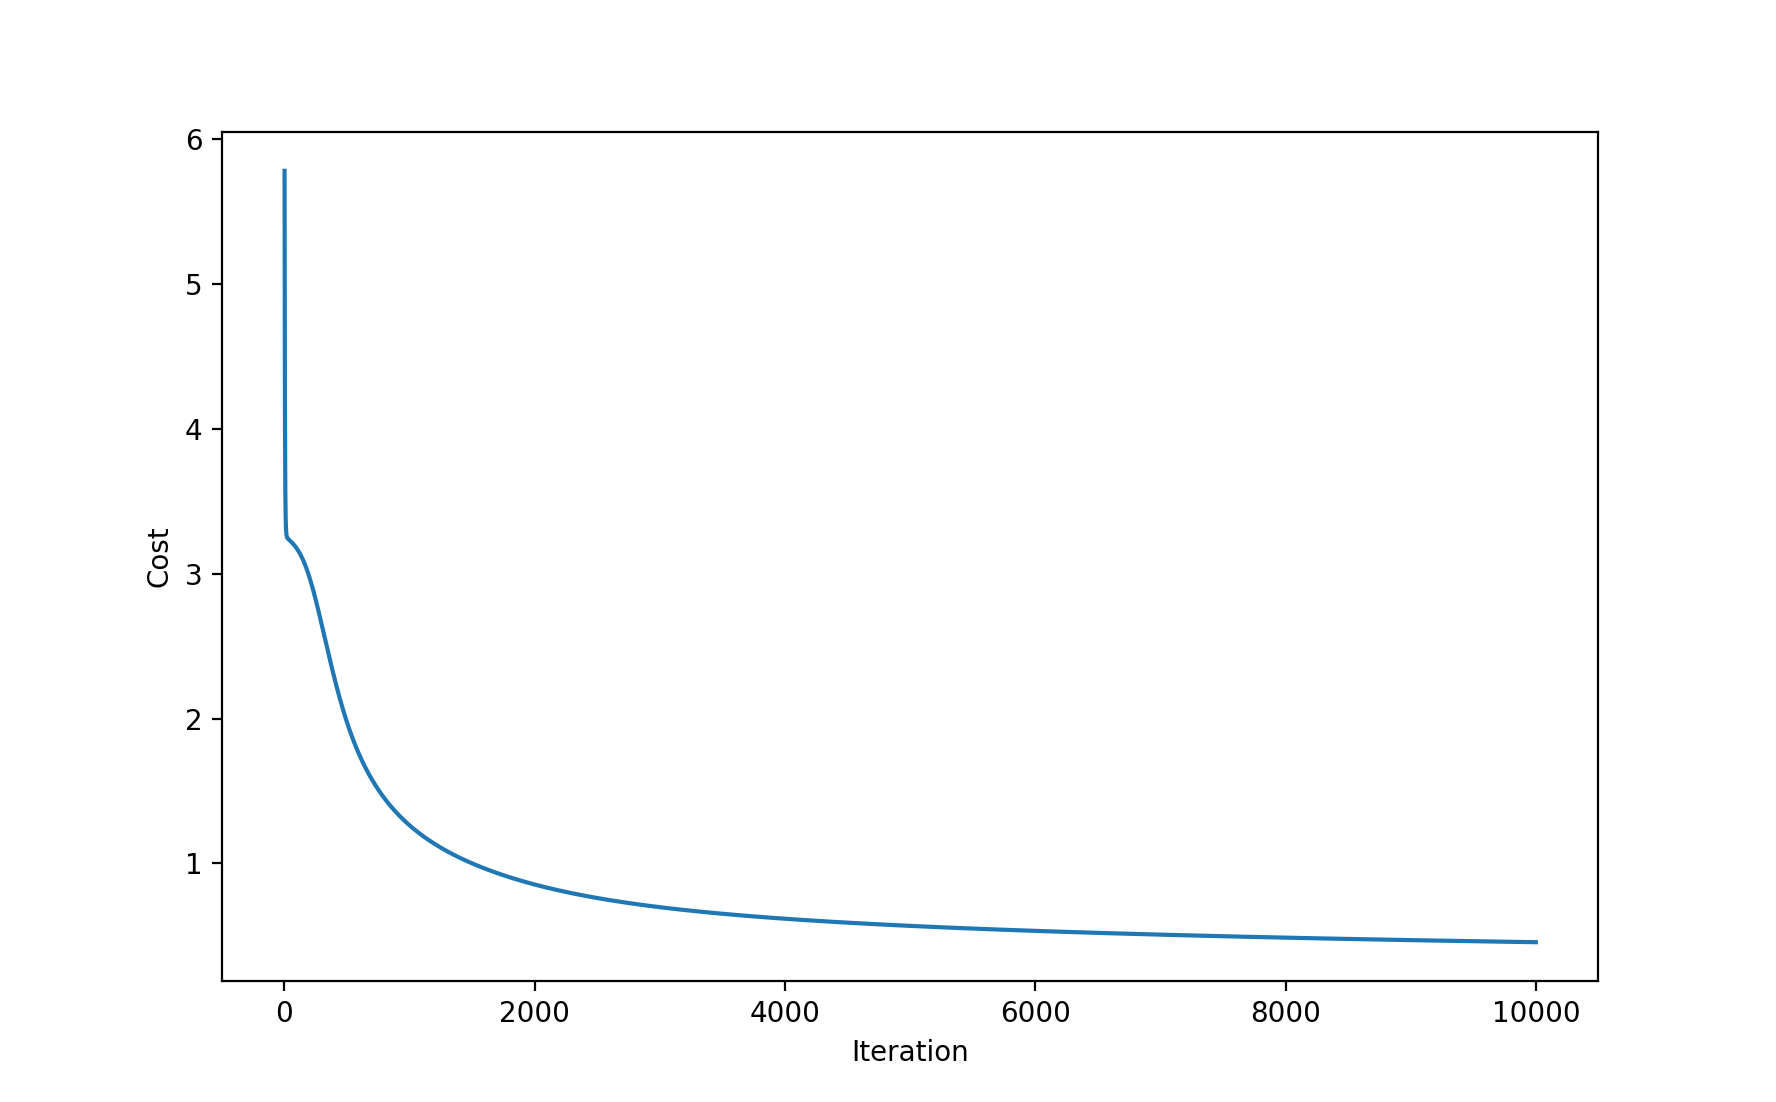
\includegraphics[width=0.5\linewidth]{figs/Chap_8_Figure_1.png}
\end{figure}

准确率如下：

\begin{table}[H]
    \centering
    \small
    \begin{tabularx}{\linewidth}{lYYYYYYYYYYY}
    \toprule
	数字 & 0 & 1 & 2 & 3 & 4 & 5 & 6 & 7 & 8 & 9 & Total \\
    \midrule
	准确率 & 98.6\% & 97.8\% & 93.4\% & 93.4\% & 97.0\% & 93.8\% & 97.8\% & 95.6\% & 95.8\% & 94.0\% & 95.7\% \\
    \bottomrule
    \end{tabularx}
\end{table}

\paragraph{附·使用 \texttt{scipy} 优化}

自己写的梯度下降跑得很慢，使用 \texttt{scipy.optimize.minimize} 来最小化 $J(\Theta)$，method 选用 $\text{CG}$，结果如下：

\begin{lstlisting}
     fun: 0.3139915007113895
     jac: array([-2.06059133e-05, -3.07615047e-11,  7.43614742e-10, ...,
       -2.86333807e-05,  4.03018555e-06,  5.10265929e-05])
 message: 'Optimization terminated successfully.'
    nfev: 1074
     nit: 461
    njev: 1074
  status: 0
 success: True
       x: array([-9.31407860e-01, -1.53807524e-07,  3.71577070e-06, ...,
       -1.27597236e-01, -1.69568829e-01,  3.47560466e-01])
\end{lstlisting}

\begin{figure}[H]
    \centering
    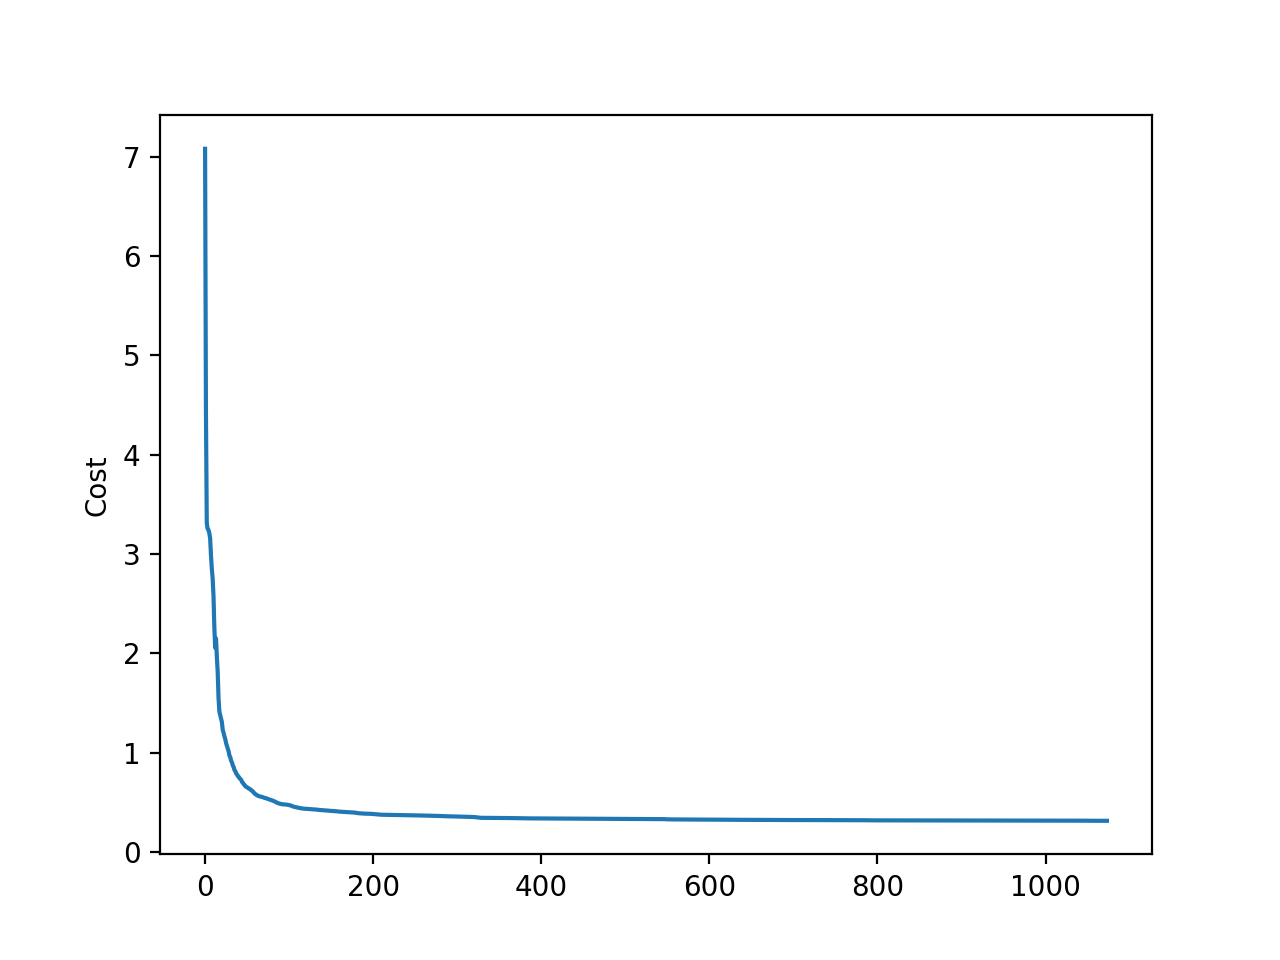
\includegraphics[width=0.5\linewidth]{figs/Chap_8_Figure_CG.png}
\end{figure}

\begin{table}[H]
    \centering
    \small
    \begin{tabularx}{\linewidth}{lYYYYYYYYYYY}
    \toprule
	数字 & 0 & 1 & 2 & 3 & 4 & 5 & 6 & 7 & 8 & 9 & Total \\
    \midrule
	准确率 & 99.8\% & 100.0\% & 99.4\% & 99.4\% & 99.2\% & 99.8\% & 99.6\% & 99.6\% & 100.0\% & 99.0\% & 99.6\% \\
    \bottomrule
    \end{tabularx}
\end{table}

当然，再次强调，由于没有划分训练集、验证集、测试集，这个准确率并不能说明问题。
 \newpage
\section{偏差与方差}
\label{sec:chapter9}

\subsection{训练集、验证集与测试集}

此前的实验使用全部数据训练模型，并在同一批数据上评估准确率。这种做法并不可靠：模型可能只是记住了训练样本，即使训练准确率很高，也可能已经发生过拟合，无法对新数据作出准确预测。正确的做法是保留一个不参与训练的独立测试集，只在模型建立完成后使用它进行最终评估，这样得到的结果才能反映模型的泛化能力。

如果模型包含需要人工选择的超参数，例如正则化参数 $\lambda$，仅划分训练集和测试集仍然不够。若反复根据测试结果选择表现最好的超参数，参数选择过程实际上也利用了测试集信息，测试集便不再真正独立。为此还要引入验证集：使用训练集拟合模型，使用验证集比较不同超参数，确定最终方案后再在测试集上评估。测试集自始至终都不参与模型训练和超参数选择。

如果训练过程包含正则项，计算训练集、验证集或测试集误差时应去除该项。正则化的作用是在训练阶段约束参数 $\theta$，帮助得到复杂度更合适的模型；而评价这个参数的实际预测效果时，真正需要衡量的是预测值与真实值之间的差异，因此应使用不含正则项的原始代价函数。

\subsection{高偏差与高方差}

模型发生欠拟合时，通常称其具有高偏差；发生过拟合时，则称其具有高方差。以多项式回归为例，随着多项式次数增加，模型表达能力逐渐增强，并由欠拟合过渡到合适拟合，最终可能出现过拟合。在这一过程中，训练误差 $J_\text{train}(\theta)$ 通常持续减小，因为更复杂的模型总能更充分地拟合训练数据；验证误差 $J_\text{valid}(\theta)$ 则会先减小后增大，在中间某个复杂度处达到最小值，如下图所示：

\begin{figure}[H]
    \centering
    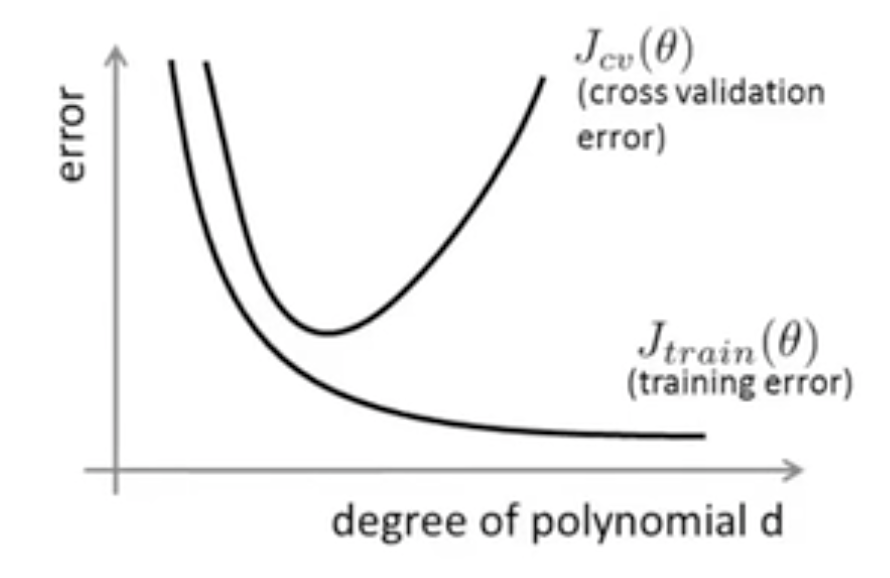
\includegraphics[width=0.4\linewidth]{figs/Chap_9_img.png}
\end{figure}

\subsection{学习曲线}

误差随训练集规模变化的曲线称为学习曲线。分别绘制训练误差与验证误差，可以观察增加训练数据时模型表现如何变化，从而帮助判断模型处于高偏差还是高方差状态。

对于高偏差模型，当训练集很小时，模型容易拟合少量样本，因此 $J_\text{train}(\theta)$ 较小，而 $J_\text{valid}(\theta)$ 较大。随着训练集增大，训练任务变得更困难，$J_\text{train}(\theta)$ 会迅速增大；$J_\text{valid}(\theta)$ 虽然有所减小，但幅度通常有限。最终二者逐渐接近，并共同稳定在较高水平，说明模型本身的表达能力不足。

对于高方差模型，训练集很小时，模型可以近乎记住所有样本，因此 $J_\text{train}(\theta)$ 很小，而 $J_\text{valid}(\theta)$ 较大。随着训练集增大，$J_\text{train}(\theta)$ 会略有上升，$J_\text{valid}(\theta)$ 会逐渐下降；但即使训练集已经较大，训练误差仍可能明显小于验证误差，二者之间保持较大间隔。

\begin{figure}[H]
    \centering
    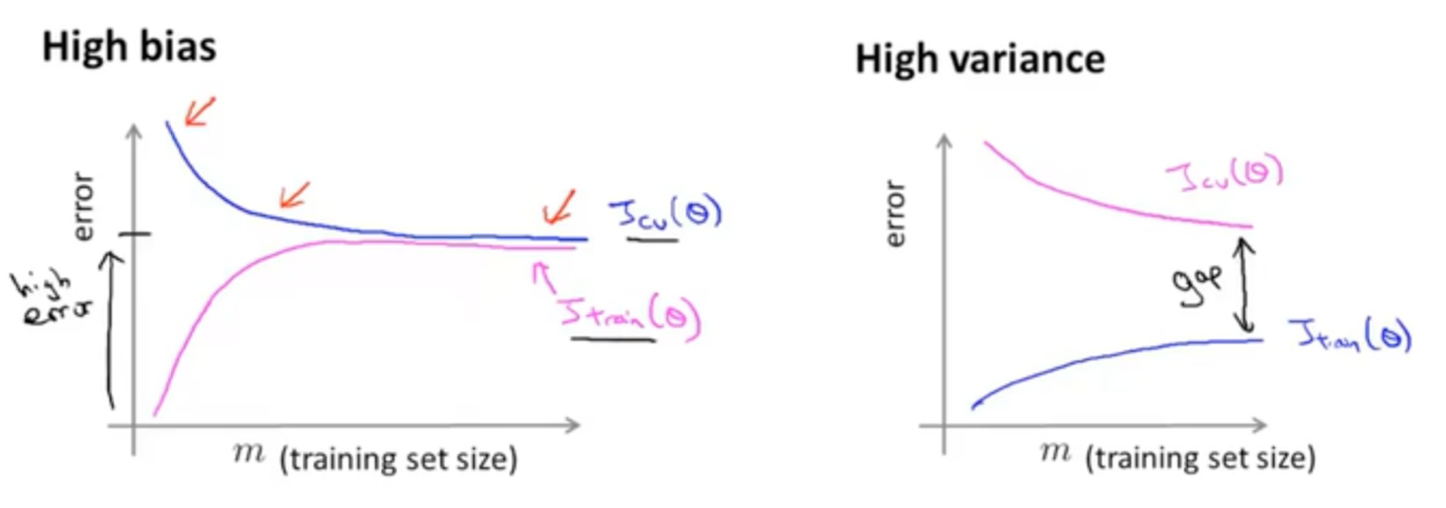
\includegraphics[width=0.8\linewidth]{figs/Chap_9_img2.png}
\end{figure}

由上述分析可知，如果模型处于高偏差状态，继续增加训练数据通常没有明显帮助，因为模型本身过于简单；更有效的方法是增加特征或提高模型复杂度。对于高方差模型，增加训练数据则可能缩小训练误差与验证误差之间的差距，从而缓解过拟合。


\subsection{代码实现}

\paragraph{正则化线性回归}

首先观察数据集：

\begin{figure}[H]
    \centering
    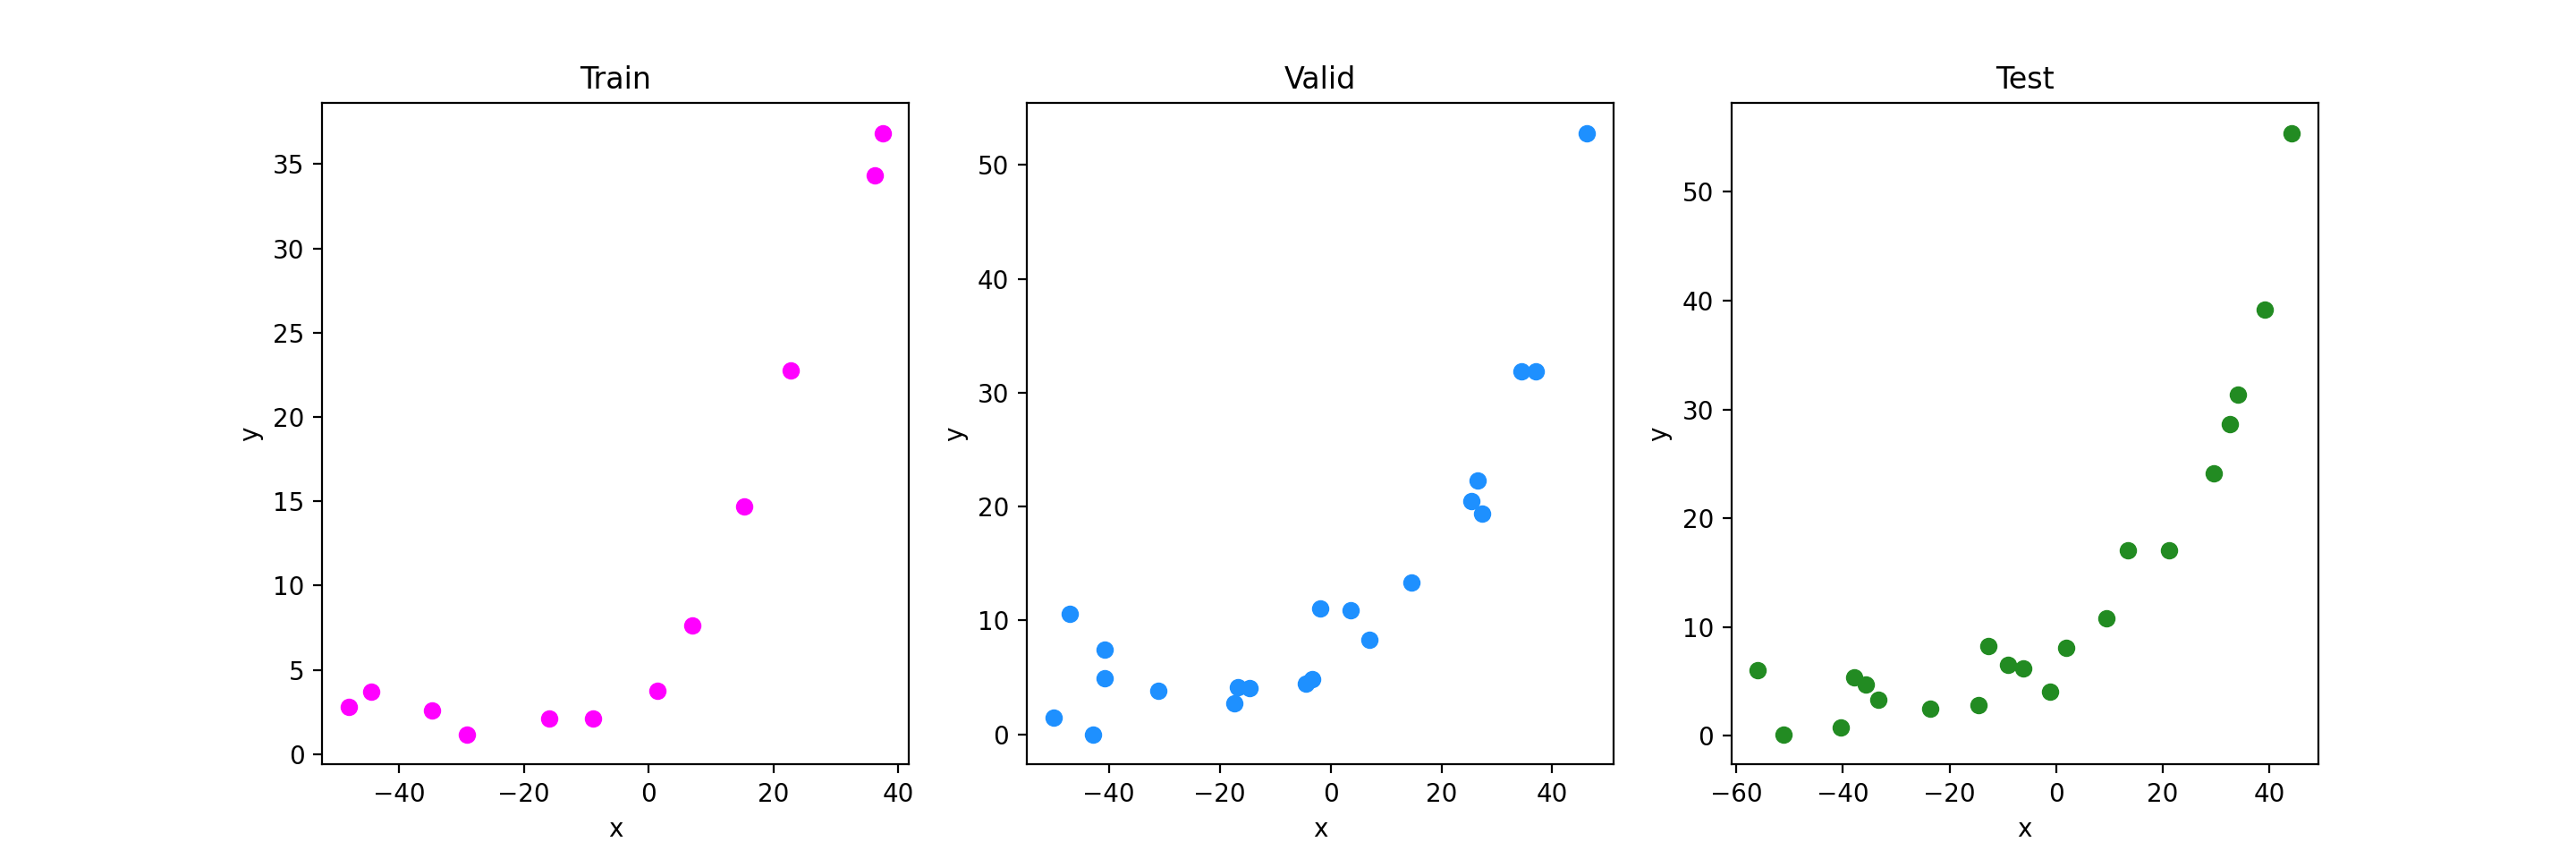
\includegraphics[width=\linewidth]{figs/Chap_9_Figure_0.png}
\end{figure}

正则化线性回归的矩阵形式为：
\begin{align*}
J(\theta)&=\frac{1}{2m}\left[\theta^TX^TX\theta-2\theta^TX^Ty+y^Ty+\lambda\hat\theta^T\hat\theta\right]\\
\frac{\partial J}{\partial \theta}&=\frac{1}{m}\left[X^TX\theta-X^Ty+\lambda\hat\theta\right]
\end{align*}

其中，$\hat\theta$ 表示将 $\theta_0$ 置为 $0$ 后的 $\theta$，因为偏置项不参与正则化。

\begin{lstlisting}[language=Python]
import numpy as np
from scipy.io import loadmat
from scipy.optimize import minimize
import matplotlib.pyplot as plt

data = loadmat('ex5data1.mat')
X, y, Xval, yval, Xtest, ytest = \
data['X'], data['y'], data['Xval'], data['yval'], data['Xtest'], data['ytest']
X = np.hstack((np.ones((X.shape[0], 1)), X))
Xval = np.hstack((np.ones((Xval.shape[0], 1)), Xval))
Xtest = np.hstack((np.ones((Xtest.shape[0], 1)), Xtest))

def unseq(theta):
	return theta.reshape(theta.shape[0], 1)

def seq(theta):
	return theta.flatten()

def J(theta, X, y, lamb):
	m = X.shape[0]
	thetahat = np.vstack((np.zeros((1, 1)), theta[1:, :]))
	return ((theta.T@X.T@X@theta-2*theta.T@X.T@y+y.T@y+lamb*thetahat.T@thetahat)/m/2)[0][0]

def partJ(theta, X, y, lamb):
	m = X.shape[0]
	thetahat = np.vstack((np.zeros((1, 1)), theta[1:, :]))
	return (X.T@X@theta-X.T@y+lamb*thetahat)/m

def Train(X, y):
	return minimize(fun = lambda theta, X, y, lamb: J(unseq(theta), X, y, lamb), 
				   x0 = np.array([1, 1]), 
				   jac = lambda theta, X, y, lamb: seq(partJ(unseq(theta), X, y, lamb)), 
				   args = (X, y, 1), 
				   method = 'CG')

res = Train(X, y)
print(res)
\end{lstlisting}

回归结果为：

\begin{lstlisting}
     fun: 22.3795418229475
     jac: array([ 3.74520898e-06, -1.25949765e-07])
 message: 'Optimization terminated successfully.'
    nfev: 28
     nit: 18
    njev: 28
  status: 0
 success: True
       x: array([13.08771802,  0.36774202])
\end{lstlisting}

回归曲线如下：

\begin{figure}[H]
    \centering
    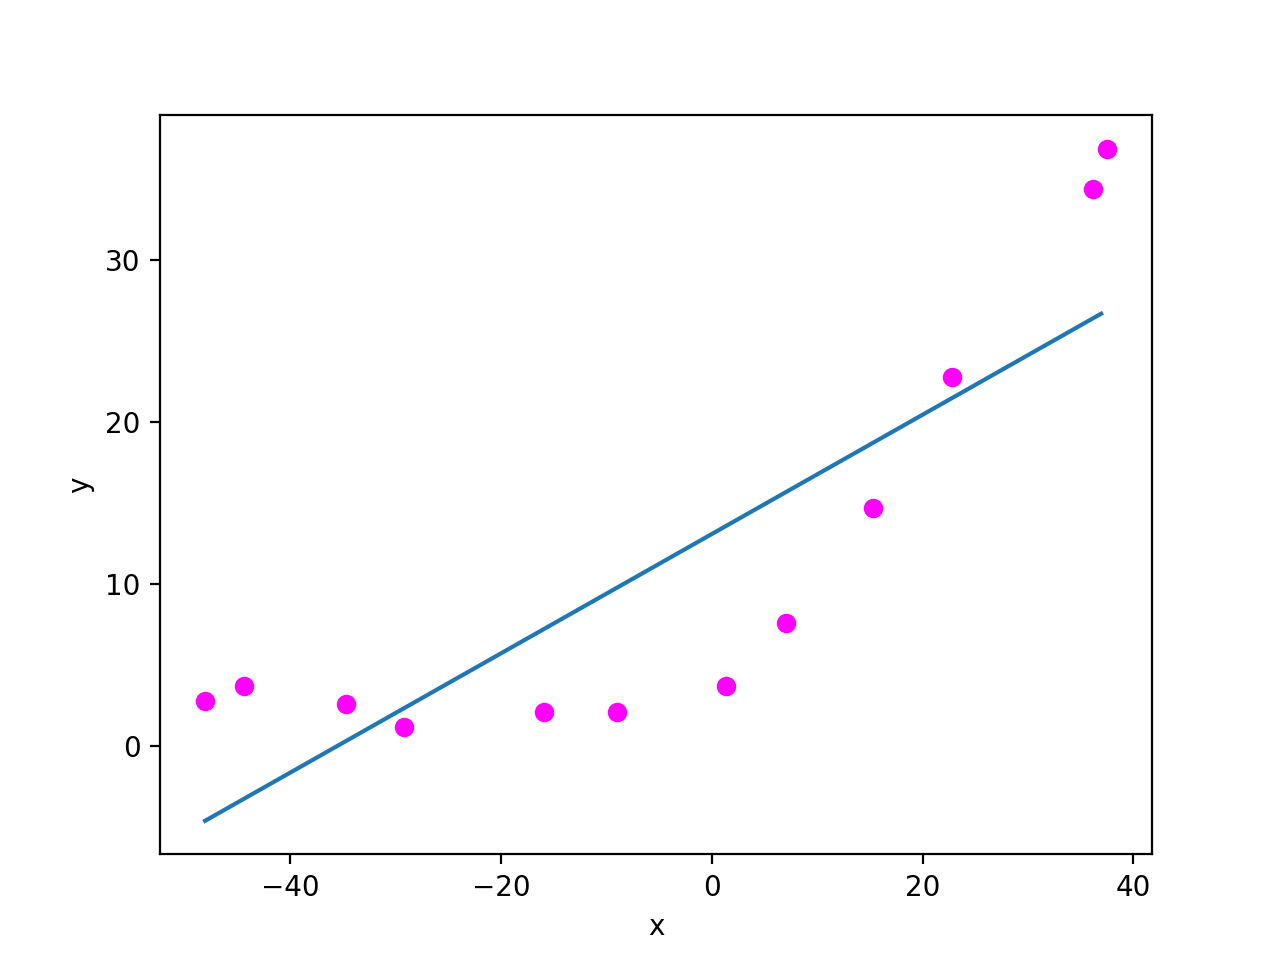
\includegraphics[width=0.5\linewidth]{figs/Chap_9_Figure_1.png}
\end{figure}


\paragraph{学习曲线的绘制}

绘制学习曲线时，依次增大训练集规模，每次重新训练参数，再分别计算当前训练子集的误差和验证集误差。需要注意，训练参数时可以使用正则化，但评估误差时应取 $\lambda=0$：

\begin{lstlisting}[language=Python]
Z_train = []
Z_valid = []
for i in range(1, 1+X.shape[0]):
	res = Train(X[:i, :], y[:i, :])
	Z_train.append(J(unseq(res.x), X[:i, :], y[:i, :], 0))
	Z_valid.append(J(unseq(res.x), Xval, yval, 0))

ax = plt.subplot(1, 1, 1)
ax.set_xlabel('size of training set')
ax.set_ylabel('Cost')
ax.set_title('learning curves')
ax.plot(range(1, 1+len(Z_train)), Z_train, color='darkviolet', label='Train')
ax.plot(range(1, 1+len(Z_valid)), Z_valid, color='tomato', label='Validation')
ax.legend()
plt.show()
\end{lstlisting}

作图如下：

\begin{figure}[H]
    \centering
    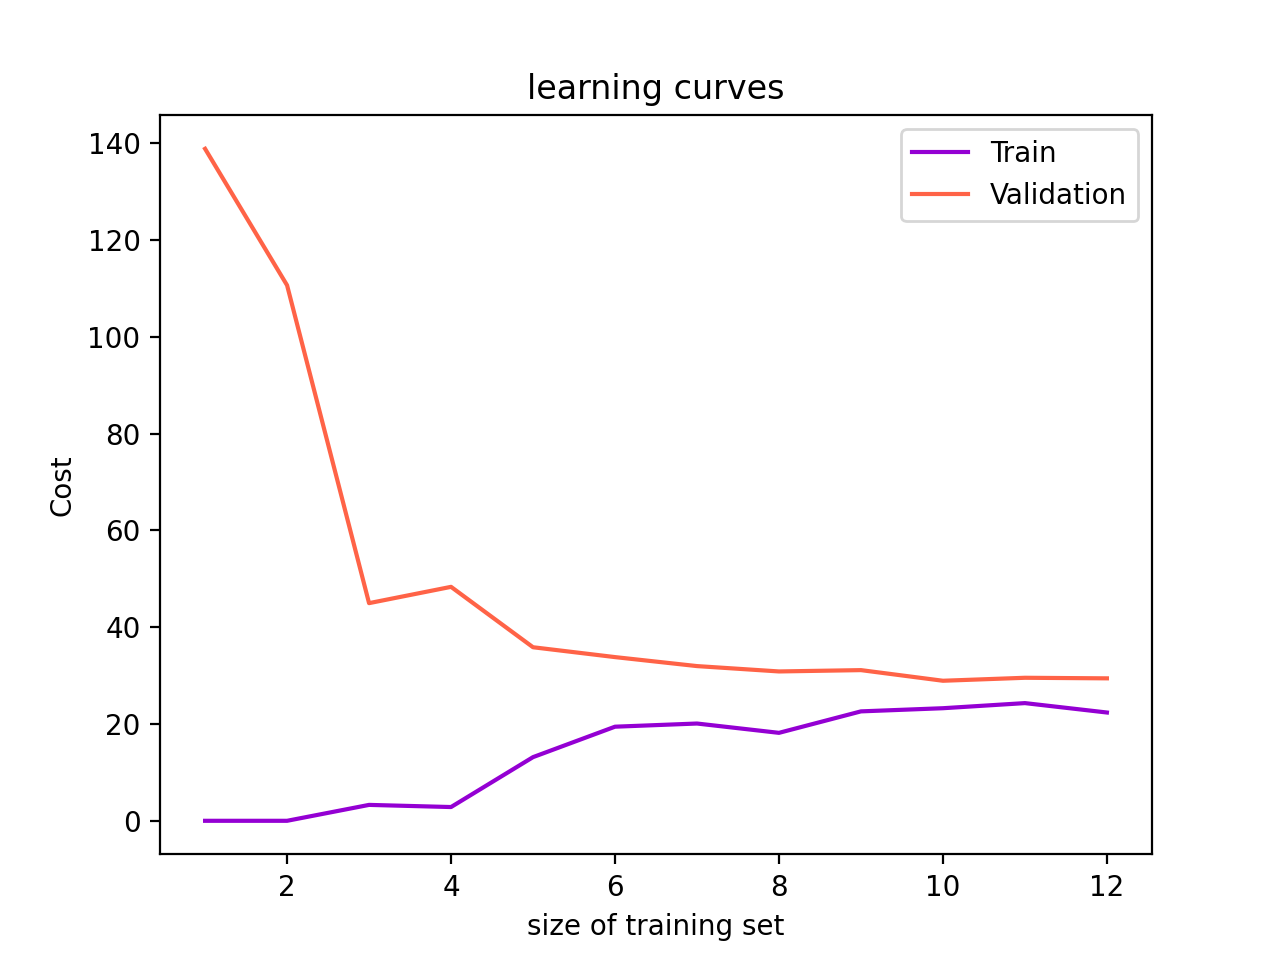
\includegraphics[width=0.5\linewidth]{figs/Chap_9_Figure_2.png}
\end{figure}

图中训练误差和验证误差都较大，并且随着样本数量增加逐渐接近。这是典型的高偏差学习曲线，说明当前线性模型发生了欠拟合。

\paragraph{多项式回归}

欠拟合的主要原因是当前使用了线性回归，而数据明显呈现非线性关系。为了提高模型的表达能力，下面引入高次特征，改用多项式回归。

加入高次特征后，特征取值范围会随着次数迅速增大，不同维度的尺度可能相差悬殊。为了保证优化过程稳定，需要对扩展后的特征进行标准化：

\begin{lstlisting}[language=Python]
data = loadmat('ex5data1.mat')
X, y, Xval, yval, Xtest, ytest = \
data['X'], data['y'], data['Xval'], data['yval'], data['Xtest'], data['ytest']

dim = 9
meanX, stdX = [], []
meany, stdy = 0, 0

def featurePrepare(X, y):
	"""
	feature extension & normalization
	"""
	global meanX, stdX, meany, stdy
	res = np.empty((X.shape[0], 0))
	for i in range(dim):
		tmpX = X ** i
		meanX.append(np.mean(tmpX, axis=0))
		stdX.append(np.std(tmpX, axis=0))
		if i:
			tmpX = (tmpX - meanX[i]) / stdX[i] if stdX[i] else tmpX - meamX[i]
		res = np.hstack((res, tmpX))
	meany = np.mean(y, axis=0)
	stdy = np.std(y, axis=0)
	y = (y - meany) / stdy if stdy else y - meany
	return res, y
\end{lstlisting}

首先使用最高次数为 $8$ 的多项式，并取正则化参数 $\lambda=0$. 此时模型具有较强表达能力，但完全没有正则化约束。拟合结果和学习曲线如下：

\begin{figure}[H]
    \centering
    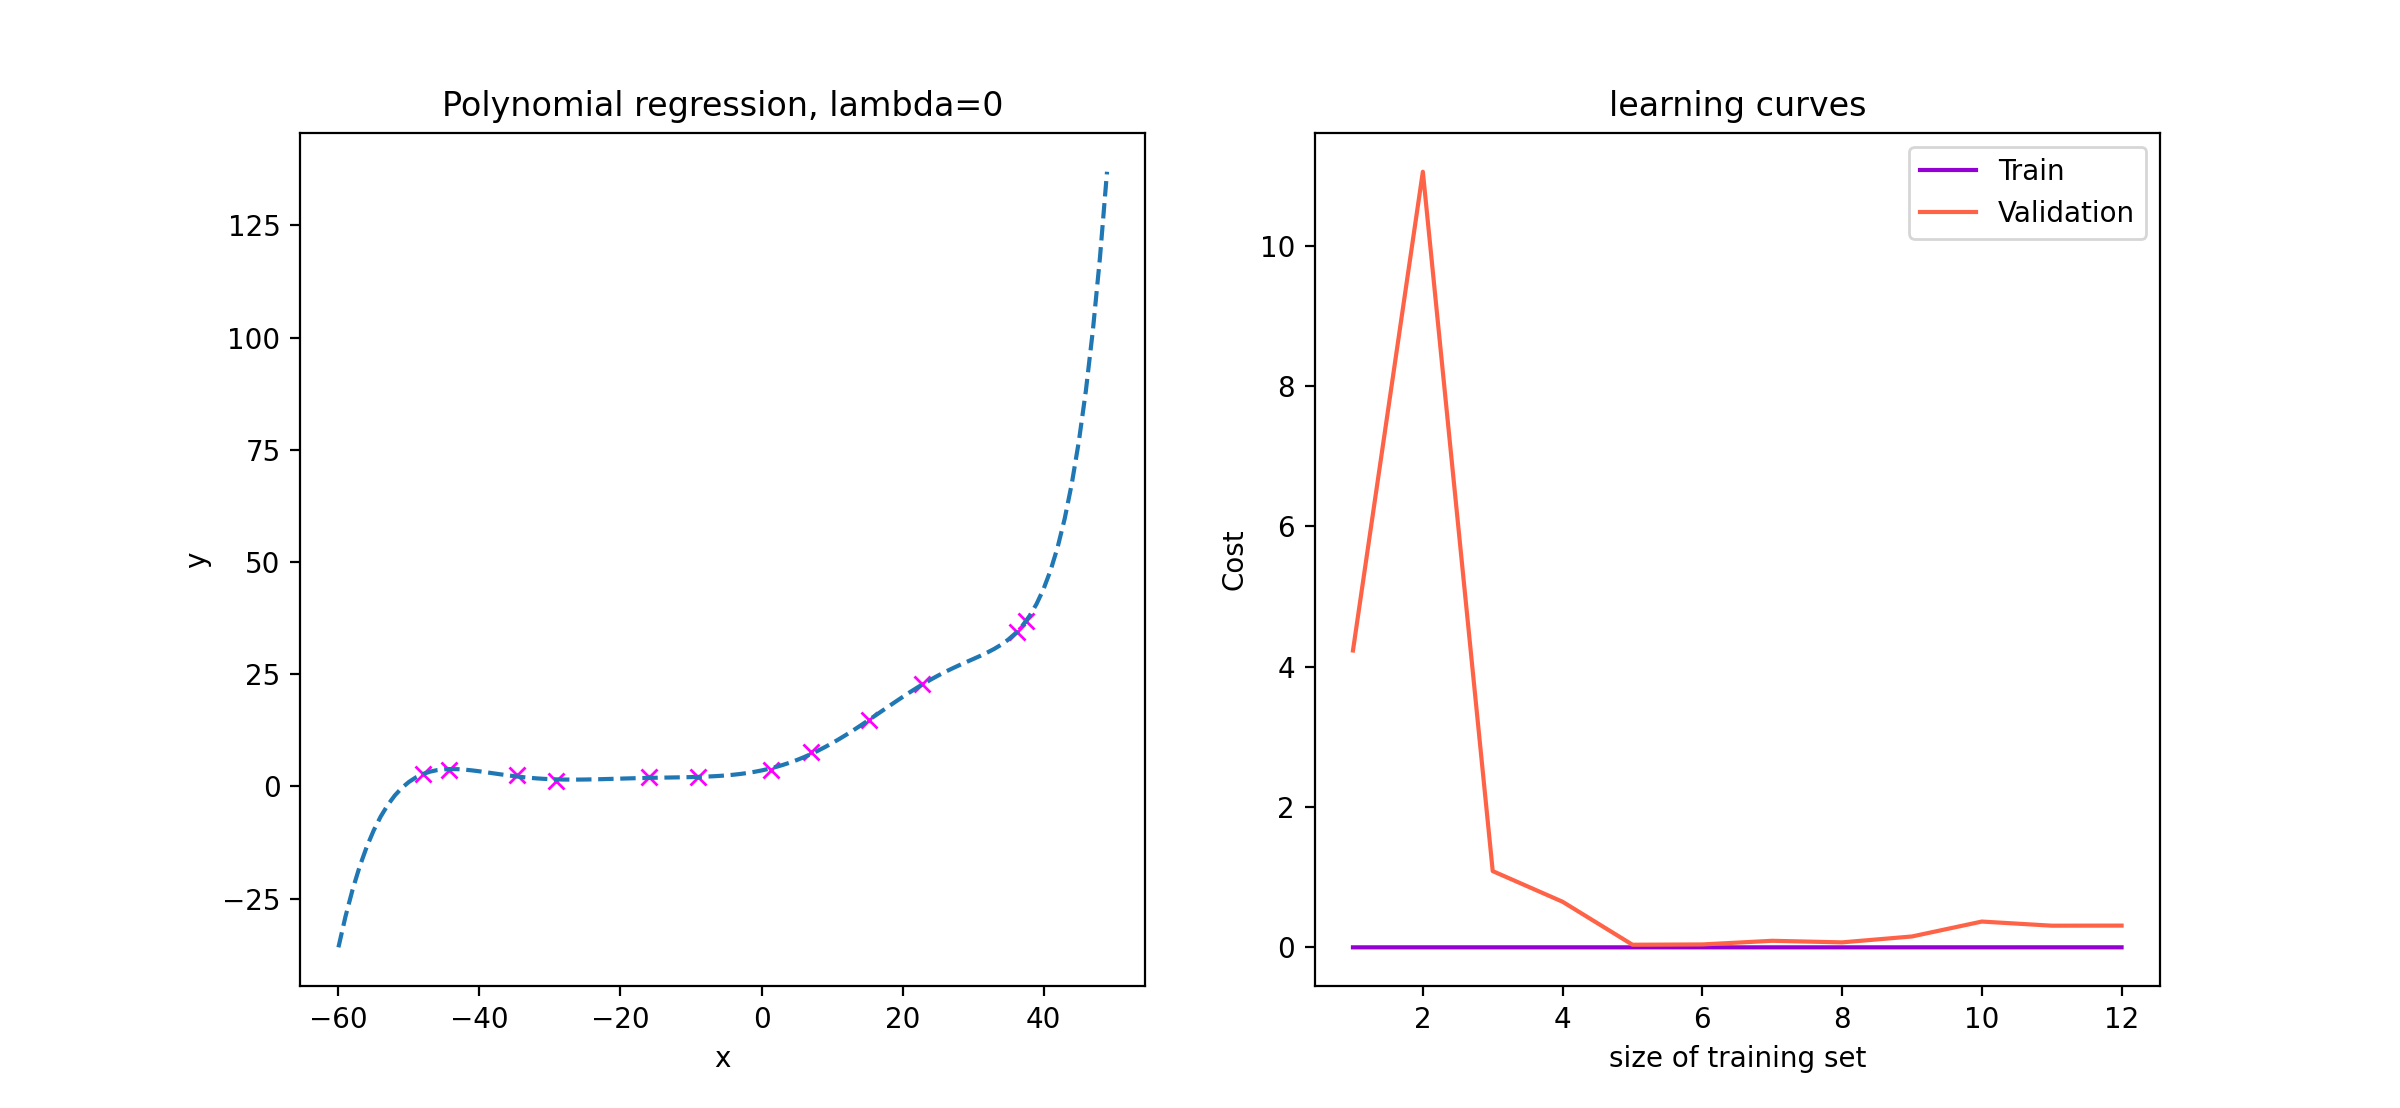
\includegraphics[width=0.8\linewidth]{figs/Chap_9_Figure_4.png}
\end{figure}
此时模型出现过拟合。

取 $\lambda=1$，得到拟合效果和学习曲线如下：
\begin{figure}[H]
    \centering
    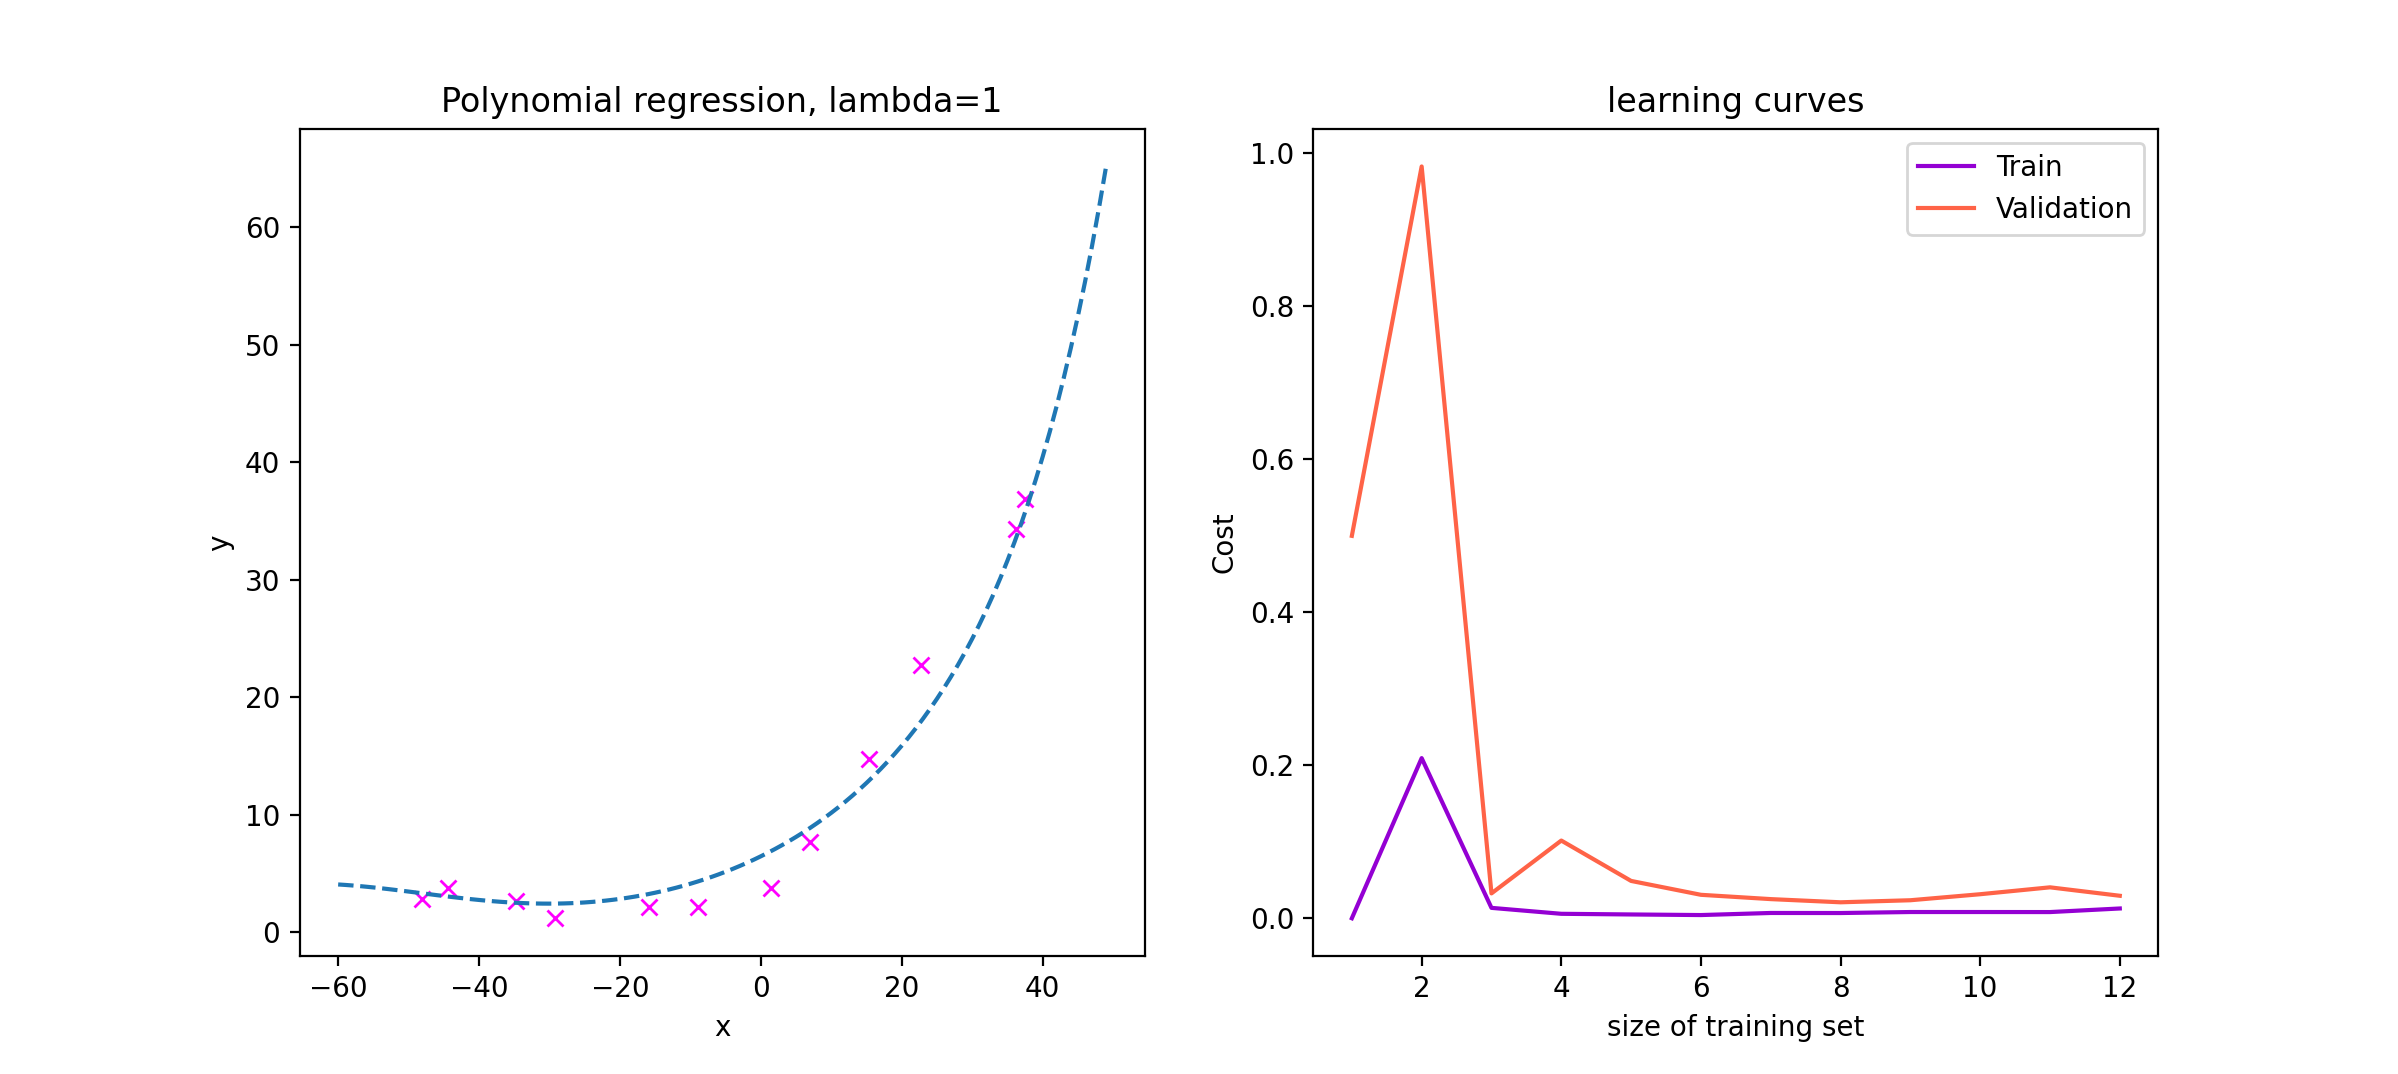
\includegraphics[width=0.8\linewidth]{figs/Chap_9_Figure_5.png}
\end{figure}
取 $\lambda=50$，得到拟合效果和学习曲线如下：
\begin{figure}[H]
    \centering
    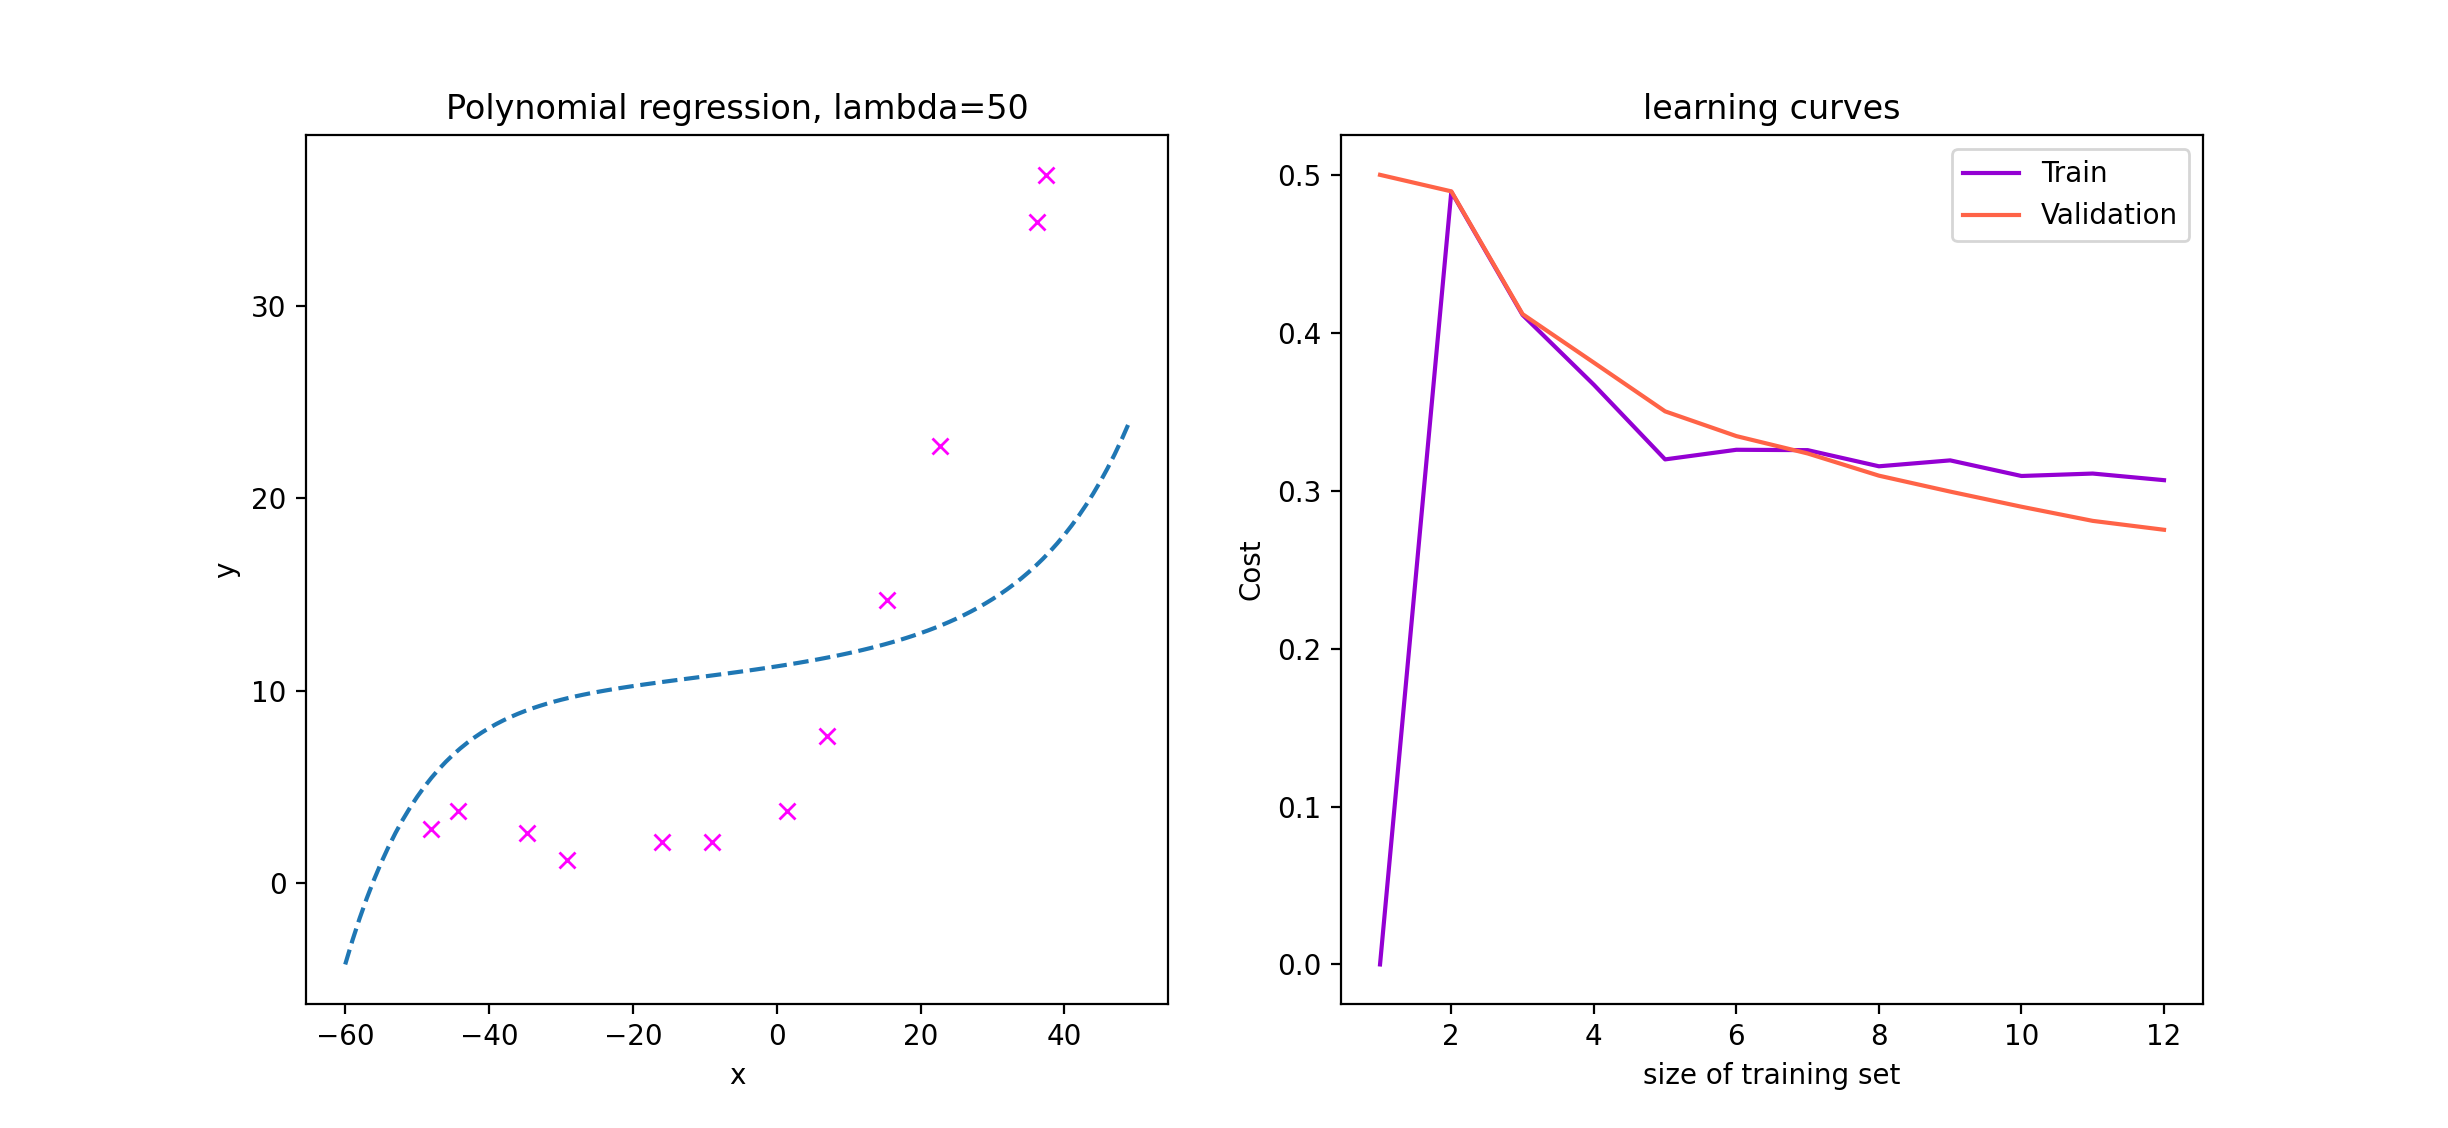
\includegraphics[width=0.8\linewidth]{figs/Chap_9_Figure_6.png}
\end{figure}
此时模型出现欠拟合。

为了系统选择正则化参数，接下来依次使用若干 $\lambda$ 训练模型，结果如下：

\begin{figure}[H]
    \centering
    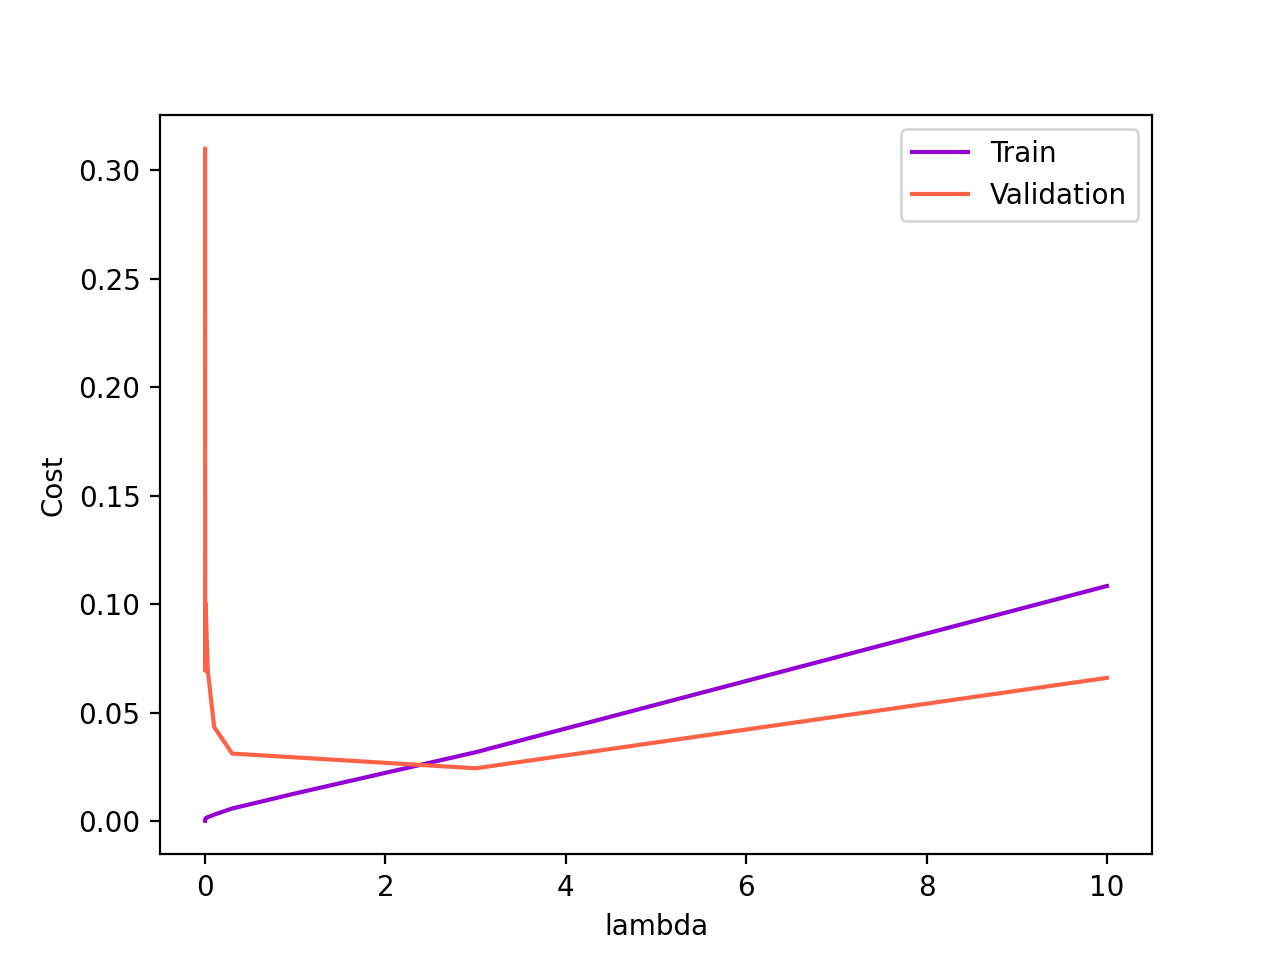
\includegraphics[width=0.5\linewidth]{figs/Chap_9_Figure_7.png}
\end{figure}

由图可见，较小的 $\lambda$ 容易产生高方差，较大的 $\lambda$ 又会带来高偏差；当 $\lambda=3$ 时验证误差最小，因此最终选取 $\lambda=3$. 
此时测试误差为 $J_\text{test}(\theta)=0.01393303991254464$. 
 \newpage
\section{支持向量机}
\label{sec:chapter10}

\subsection{优化目标}

逻辑回归的优化目标为：
\[
\min_\theta\frac{1}{m}\left[\sum_{i=1}^my^{(i)}\left(-\ln h_\theta(x^{(i)})\right)+(1-y^{(i)})\left(-\ln (1-h_\theta(x^{(i)}))\right)\right]+\frac{\lambda}{2m}\sum_{j=1}^n\theta_j^2
\]
将 $-\ln h_\theta(x^{(i)})$ 记为 $\text{cost}_1(\theta^T x^{(i)})$，它表示样本类别为 $1$ 时的代价；将 $-\ln(1-h_\theta(x^{(i)}))$ 记为 $\text{cost}_0(\theta^T x^{(i)})$，它表示类别为 $0$ 时的代价。支持向量机不再通过 sigmoid 函数得到平滑的对数代价，而使用如下分段线性函数近似：
\[
\text{cost}_1(z)=\begin{cases}0&z\geqslant1\\k_1(z-1)&z<1\end{cases}\quad\quad
\text{cost}_0(z)=\begin{cases}0&z\leqslant-1\\k_0(z+1)&z>-1\end{cases}
\]

\begin{figure}[H]
    \centering
    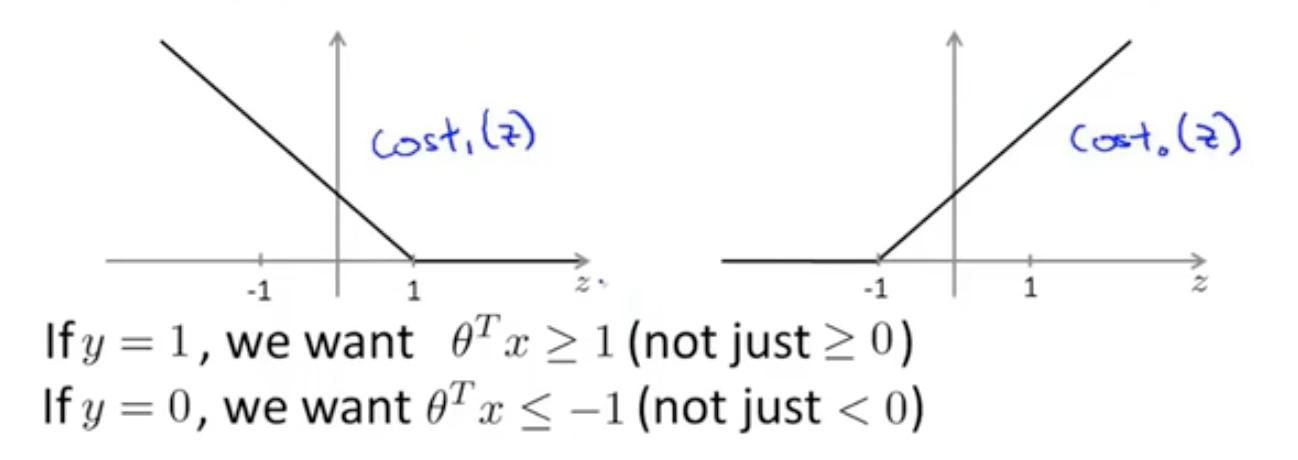
\includegraphics[width=0.6\linewidth]{figs/Chap_10_cost.png}
\end{figure}

在支持向量机的常用写法中，通常省略除以样本数 $m$ 的系数，并将正则化参数置于第一项而不是第二项。故支持向量机的优化目标为：
\[
\boxed
{\min_\theta C\sum_{i=1}^m\left[y^{(i)}\text{cost}_1(\theta^Tx^{(i)})+(1-y^{(i)})\text{cost}_0(\theta^Tx^{(i)})\right]+\frac{1}{2}\sum_{j=1}^n\theta_j^2}
\]
其中，$C$ 是正则化参数，用于权衡分类误差与参数规模，其作用与逻辑回归中的 $\frac{1}{\lambda}$ 类似：$C$ 越大，对训练样本分类错误的惩罚越强。

\begin{remark}
先考察 $y\text{cost}_1(\theta^Tx)+(1-y)\text{cost}_0(\theta^Tx)$ 这一分类代价。理想情况下，希望 $\text{cost}_y(\theta^T x)=0$，这对应 $\begin{cases}\theta^Tx\geqslant 1&\text{if }y=1\\\theta^Tx\leqslant -1&\text{if }y=0\end{cases}$. 以类别 $1$ 为例，逻辑回归只需要比较 $\theta^Tx$ 与 $0$ 的大小便可作出分类，而支持向量机还要求 $\theta^Tx$ 至少达到 $1$. 这意味着样本不仅要位于决策边界正确的一侧，还要与边界保持一定间隔。

从几何角度看，$\theta^Tx$ 是向量 $\theta$ 与 $x$ 的点积，可以理解为 $x$ 在 $\theta$ 方向上的投影与 $\theta$ 长度的乘积。$||\theta||$ 表示参数向量的长度，而正则化项 $\sum\limits_{j=1}^n\theta_j^2$ 等于 $||\theta||$ 的平方。减小参数长度相当于增大决策边界两侧的几何间隔，因此第二项体现了最大间隔的目标。$C$ 较大时，模型更重视让训练样本满足分类条件，即使这需要较大的参数；$C$ 较小时，模型允许少量样本被错误分类或落入间隔内部，以换取更大的分类间隔和更强的正则化。

\begin{figure}[H]
    \centering
    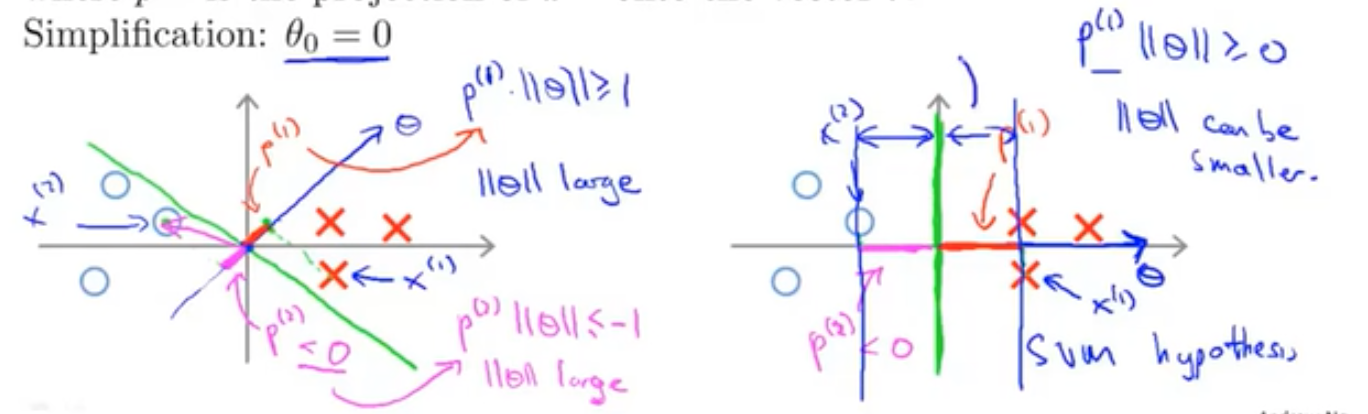
\includegraphics[width=\linewidth]{figs/Chap_10_big_margin.png}
\end{figure}

\end{remark}


\subsection{核函数}

对于在原特征空间中无法用直线或超平面分开的数据，可以引入核函数 $\phi:x\mapsto \phi(x)$，将原始 $n$ 维向量映射到更高维的特征空间。原空间中的非线性边界可能对应新空间中的线性边界，因此仍可使用线性支持向量机进行分类。常用核函数包括：

\textbf{线性核}：保持原特征不变
\[
\phi(x_i)=x_i
\]

\textbf{高斯核}
\[
\phi(x)=\begin{bmatrix}\exp\left(-||x-l^{(1)}||^2/2\sigma^2\right)\\\exp\left(-||x-l^{(2)}||^2/2\sigma^2\right)\\\vdots\\\exp\left(-||x-l^{(m)}||^2/2\sigma^2\right)\end{bmatrix}
\]
其中 $\sigma$ 控制相似度随距离衰减的速度，$l^{(1)},\cdots,l^{(m)}$ 称为 landmark. 每个新特征衡量输入 $x$ 与某个 landmark 的接近程度；实践中通常直接采用训练样本 $x^{(1)},\cdots,x^{(m)}$ 作为 landmark.


\subsection{代码实现}

\paragraph{线性可分情形}

首先观察数据集：

\begin{figure}[H]
    \centering
    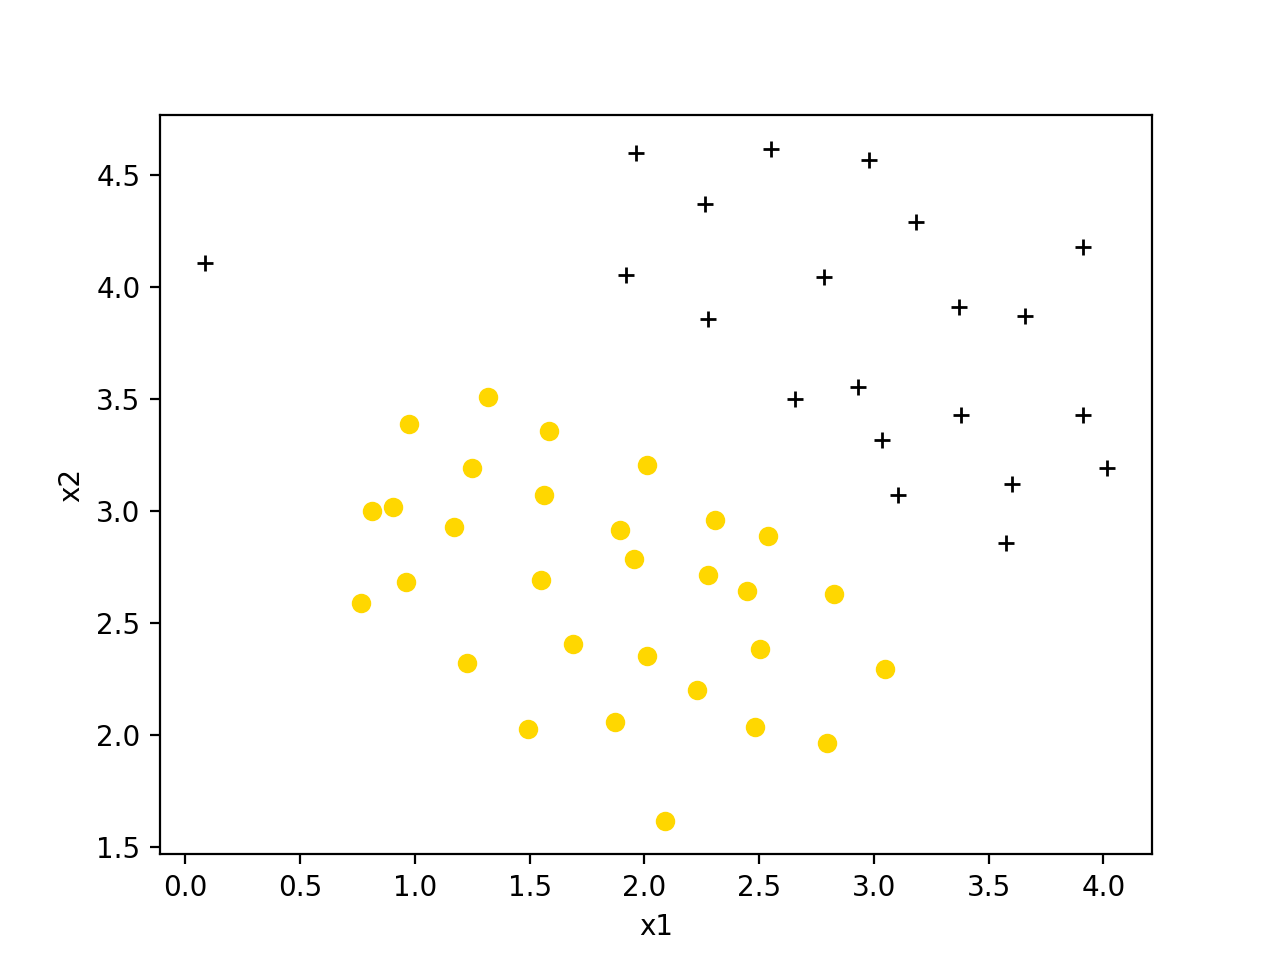
\includegraphics[width=0.4\linewidth]{figs/Chap_10_Figure_1.png}
\end{figure}

\begin{lstlisting}[language=Python]
from sklearn import svm

clf = svm.SVC(C=1, kernel='linear')
clf.fit(X, y)
\end{lstlisting}

训练结果如下：

\begin{figure}[H]
    \centering
    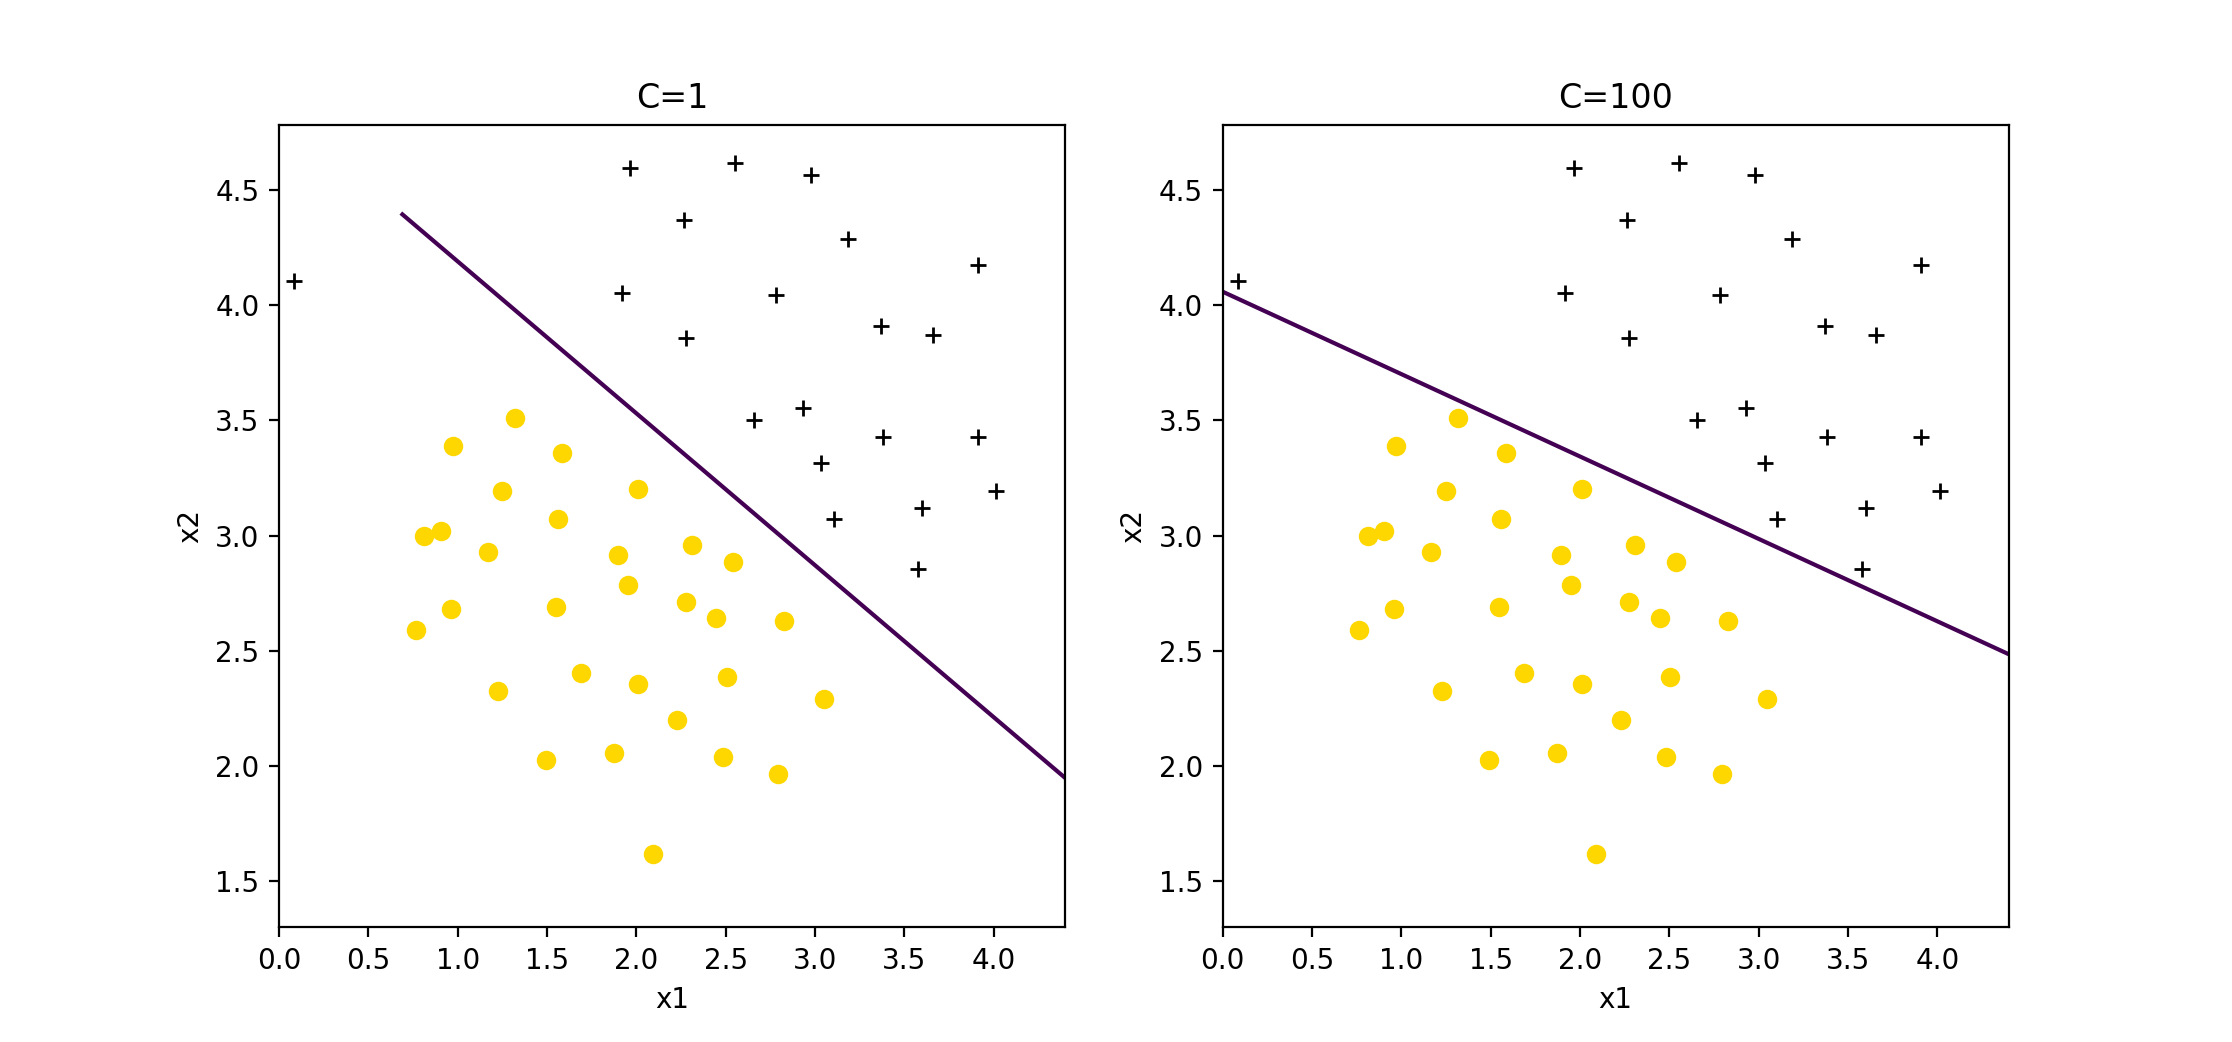
\includegraphics[width=0.8\linewidth]{figs/Chap_10_Figure_1_1.png}
\end{figure}


\paragraph{带高斯核的 SVM}

首先观察数据集：

\begin{figure}[H]
    \centering
    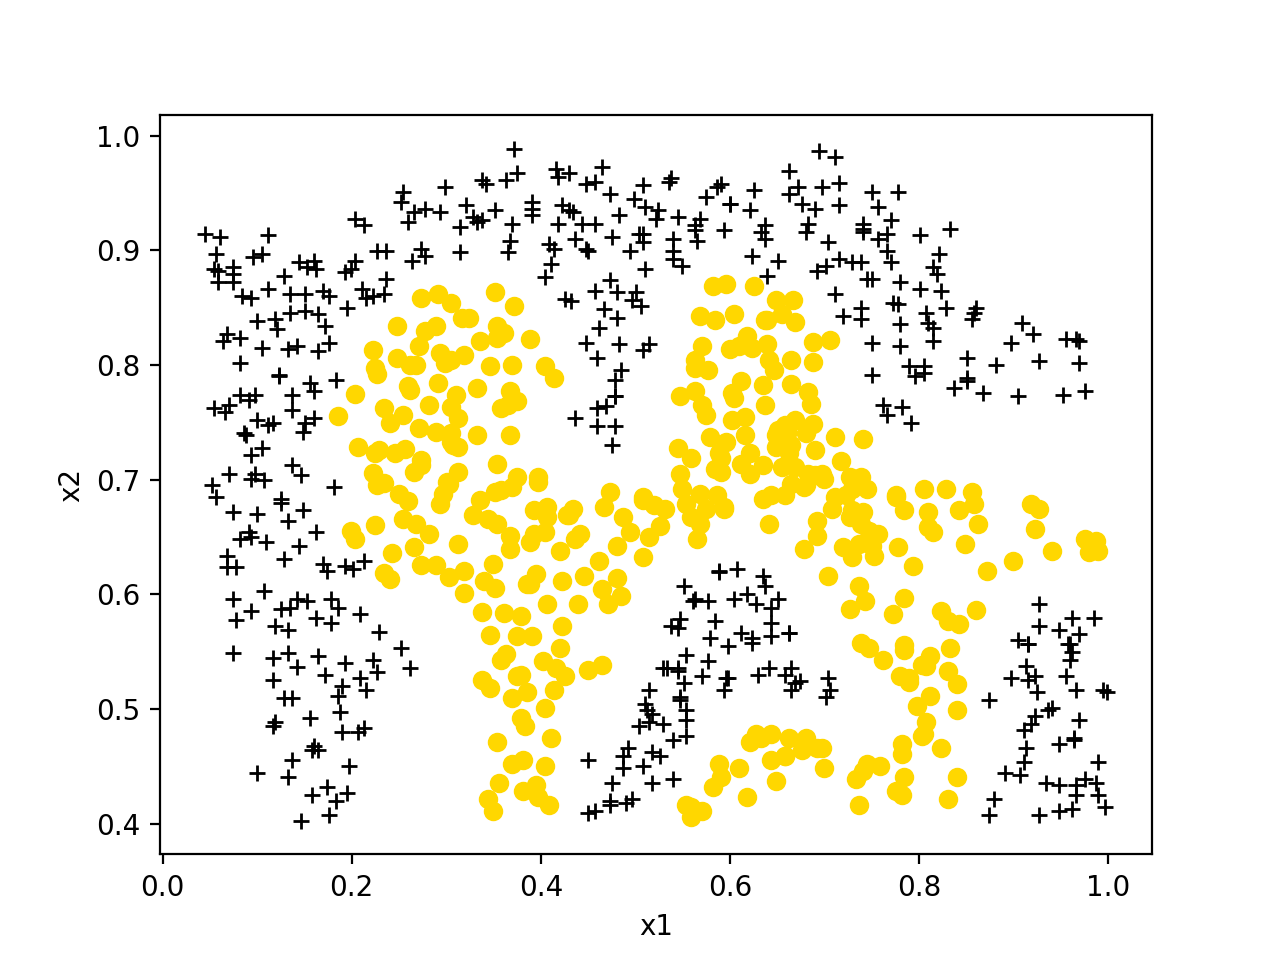
\includegraphics[width=0.4\linewidth]{figs/Chap_10_Figure_2.png}
\end{figure}

\begin{lstlisting}[language=Python]
from sklearn import svm

clf = svm.SVC(C=100, kernel='rbf', gamma=10, probability=True)
clf.fit(X, y)
\end{lstlisting}

训练结果如下：

\begin{figure}[H]
    \centering
    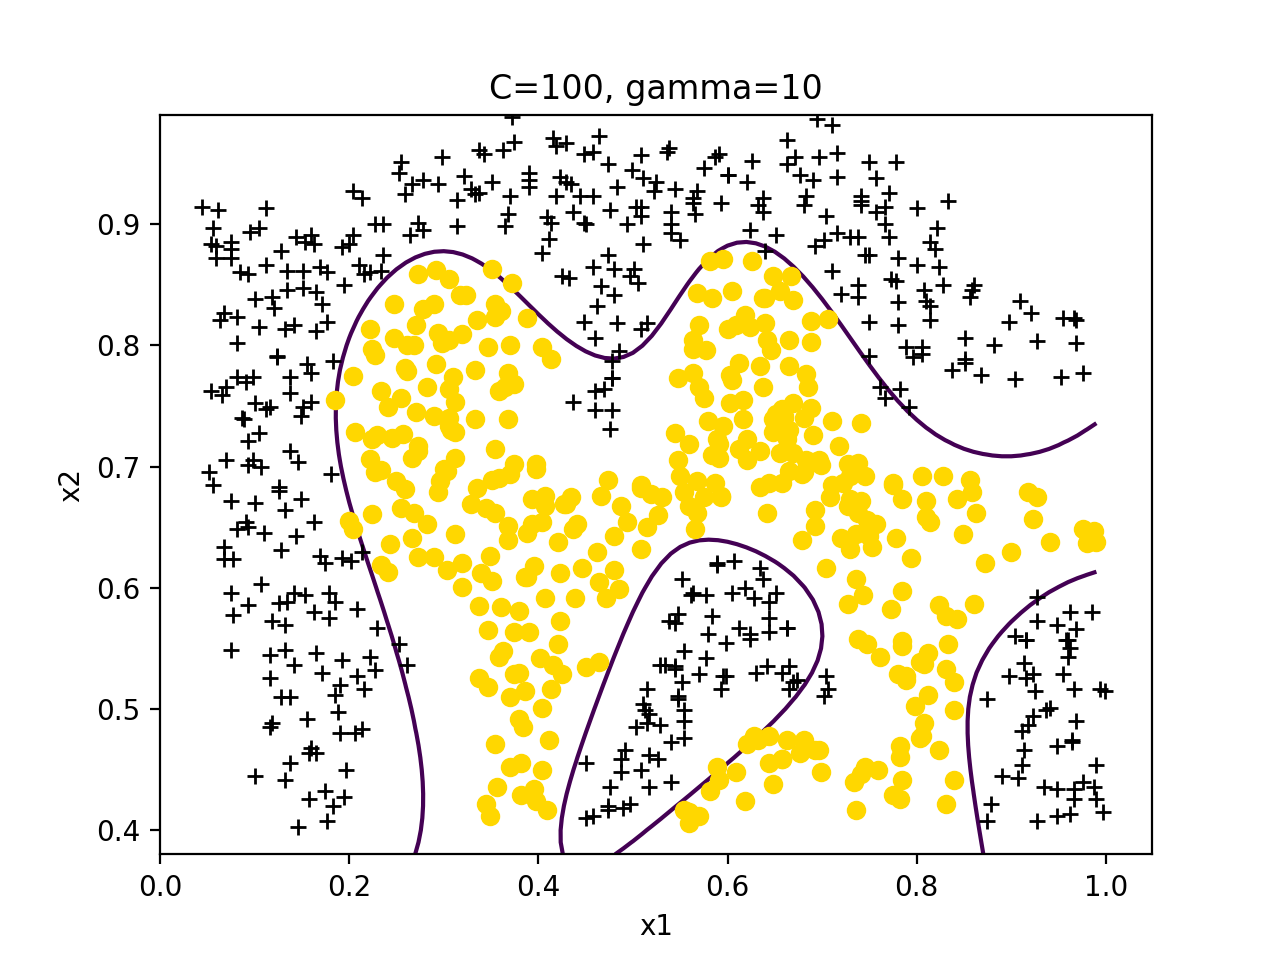
\includegraphics[width=0.4\linewidth]{figs/Chap_10_Figure_2_1.png}
\end{figure}


\paragraph{调整参数 $C,\sigma$}

数据集：

\begin{figure}[H]
    \centering
    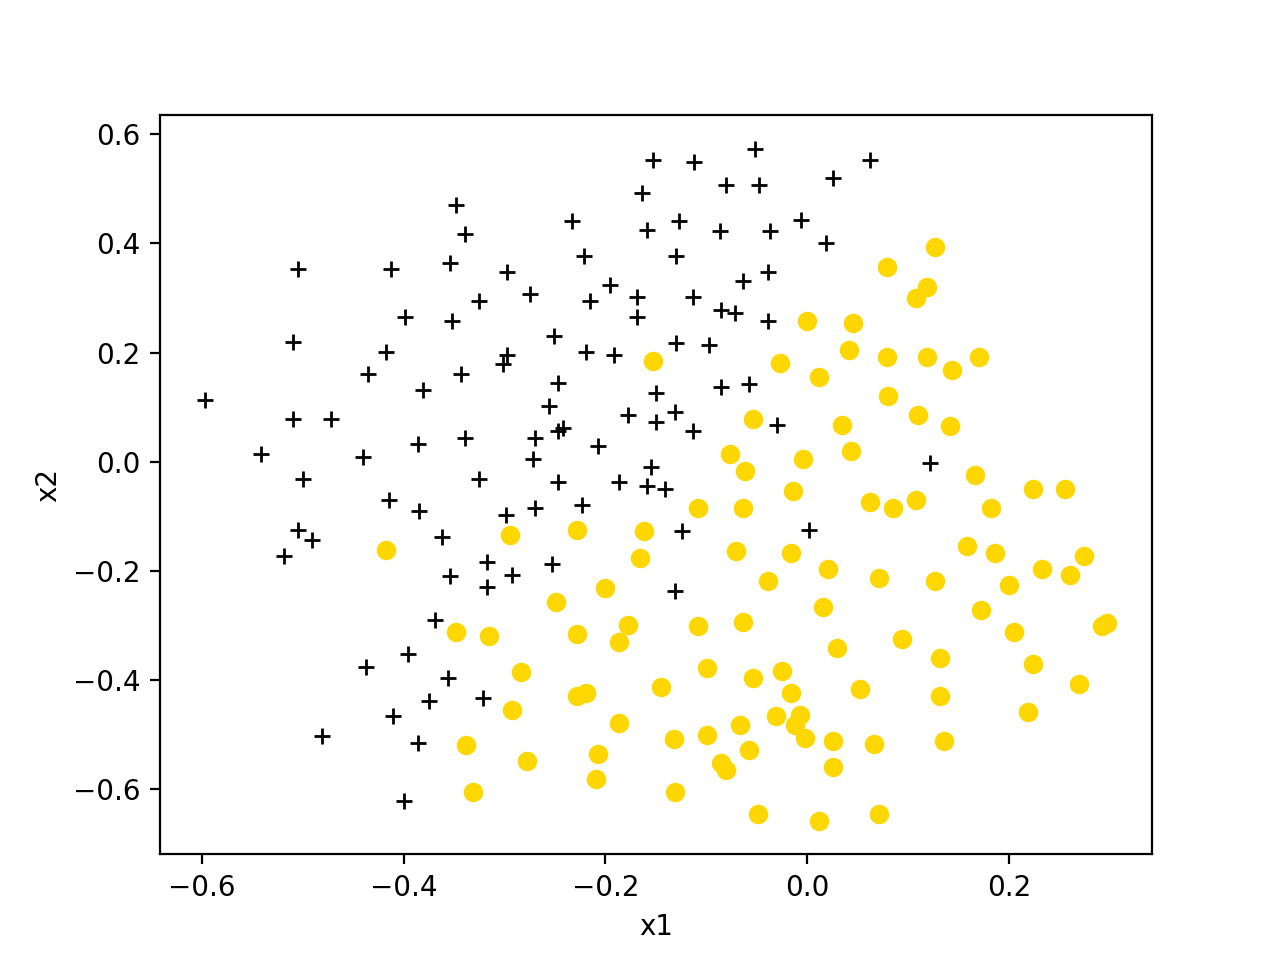
\includegraphics[width=0.4\linewidth]{figs/Chap_10_Figure_3.png}
\end{figure}

\begin{lstlisting}[language=Python]
maxscore, maxC, maxgamma = 0, 0, 0
for C in [0.01, 0.03, 0.1, 0.3, 1, 3, 10, 30]:
	for gamma in [0.01, 0.03, 0.1, 0.3, 1, 3, 10, 30]:
		clf = svm.SVC(C=C, kernel='rbf', gamma=gamma, probability=True)
		clf.fit(X, y)
		score = clf.score(X, y)
		print(C, gamma, score)
		if score > maxscore:
			maxscore, maxC, maxgamma = score, C, gamma

clf = svm.SVC(C=maxC, kernel='rbf', gamma=maxgamma, probability=True)
clf.fit(X, y)
\end{lstlisting}

训练结果如下：

\begin{figure}[H]
    \centering
    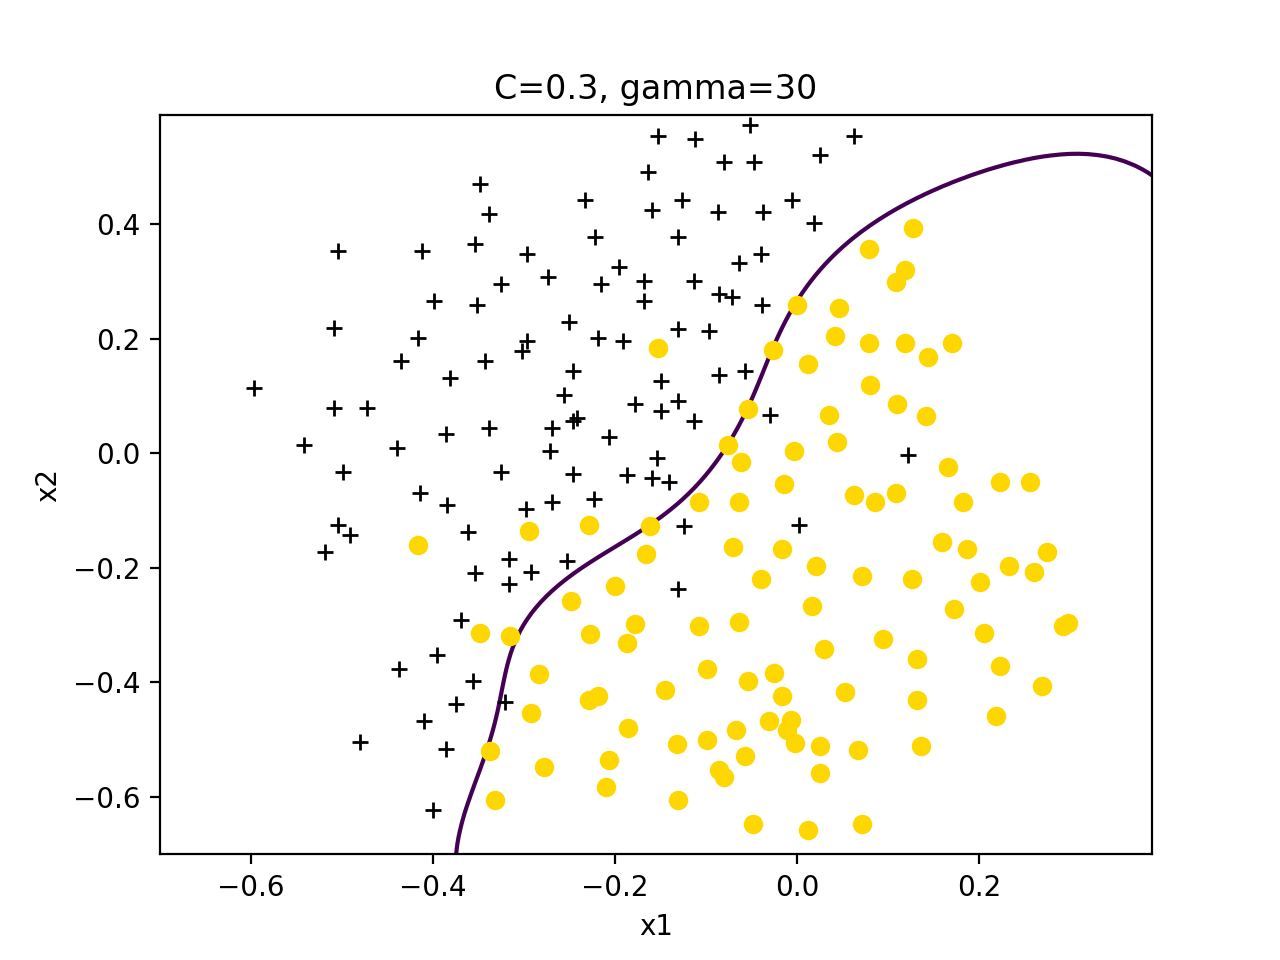
\includegraphics[width=0.4\linewidth]{figs/Chap_10_Figure_3_1.png}
\end{figure}
 \newpage
\section{K-means 聚类}
\label{sec:chapter11}

\subsection{聚类问题}

聚类问题属于无监督学习的范畴，与有监督学习不同，无监督学习的数据不再包含标注的标签。聚类问题就是在无标注的情况下将数据集分为若干类的问题。


\subsection{K-means 算法}

K-means 算法是解决聚类问题的一种算法，其基本思想非常简单：假设我们要将数据分为 $K$ 类，首先我们随机 $K$ 个聚类中心，然后反复执行以下步骤：
\begin{enumerate}
    \item 根据数据点到这 $K$ 个聚类中心的距离进行分类（距离哪个中心小就分为哪一类）；
    \item 将聚类中心重置为它所代表的那一类的所有点的平均位置。
\end{enumerate}

直到聚类中心不再改变，算法结束。

对于 K-means 算法，我们可以定义一个代价函数，为各数据点到它所属于的聚类中心的距离之平方和。很容易证明，1、2 两个步骤都是在减小这个代价，所以正确实现的 K-means 算法的代价应随着迭代次数增加而减小。

注意：
\begin{enumerate}
    \item 在实践中，我们可以任取 $K$ 个数据点作为聚类中心；
    \item 如果更新聚类中心时，没有数据属于某一聚类中心，则可以将该聚类中心删去（这样分类数会减少）或者置于随机位置上（保持分类数不变）；
    \item 执行一次 K-means 的结果依赖于聚类中心的选取方式，因此有可能得到一个局部最优解。所以我们可以多次执行算法，取代价最小的结果为最终结果。
\end{enumerate}


\subsection{代码实现}

\paragraph{平面点集分类}

首先看看数据集的样子：

\begin{figure}[H]
    \centering
    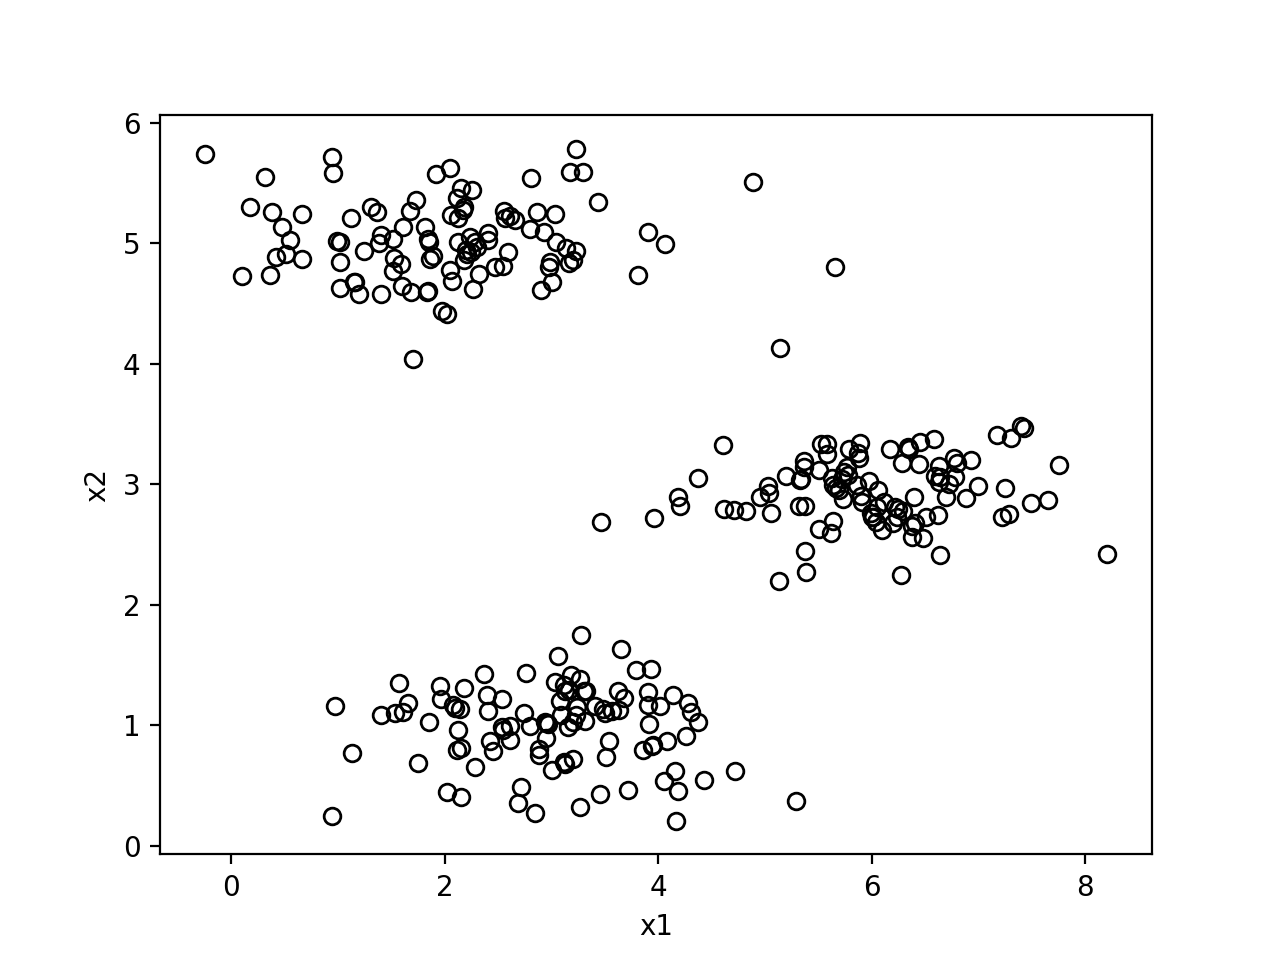
\includegraphics[width=0.5\linewidth]{figs/Chap_11_Figure_0.png}
\end{figure}

\begin{lstlisting}[language=Python]
import numpy as np
from scipy.io import loadmat
import matplotlib.pyplot as plt

X = loadmat('ex7data2.mat')['X']

def J(X, cluster, centroid):
	res = 0
	for i in range(X.shape[0]):
		res += np.dot(X[i]-centroid[cluster[i]], X[i]-centroid[cluster[i]])
	return res

def K_means(K, X, iteration=100):
	(m, n) = X.shape
	bestCluster, bestCentroid, bestJ = np.empty(m), np.empty((K, n)), np.inf
	for iter in range(iteration):
		centroid = X[np.random.randint(0, m, K)]
		cluster = np.empty(m, dtype='int')
		while True:
			ncentroid = np.zeros((K, n))
			cnt = np.zeros(K)
			for i in range(m):
				cluster[i] = np.argmin(np.sum((X[i]-centroid)**2, axis=1))
				ncentroid[cluster[i]] += X[i]
				cnt[cluster[i]] += 1
			ncentroid[cnt!=0] /= cnt[cnt!=0][:, np.newaxis]
			ncentroid[cnt==0] = X[np.random.randint(0, m, len(cnt[cnt==0]))]
			if (centroid == ncentroid).all():
				break
			centroid = ncentroid.copy()
		cost = J(X, cluster, centroid)
		if cost < bestJ:
			bestCluster, bestCentroid, bestJ = cluster.copy(), centroid.copy(), cost.copy()
	return bestCluster, bestCentroid

cl, ce = K_means(3, X, iteration=100)

ax = plt.subplot(1, 1, 1)
ax.set_xlabel('x1')
ax.set_ylabel('x2')
ax.plot(X[cl==0][:, 0], X[cl==0][:, 1], 'o', color='blue', markerfacecolor='none', alpha=0.4)
ax.plot(X[cl==1][:, 0], X[cl==1][:, 1], 'o', color='green', markerfacecolor='none', alpha=0.4)
ax.plot(X[cl==2][:, 0], X[cl==2][:, 1], 'o', color='red', markerfacecolor='none', alpha=0.4)
ax.plot(ce[0, 0], ce[0, 1], '*', color='blue', ms=10)
ax.plot(ce[1, 0], ce[1, 1], '*', color='green', ms=10)
ax.plot(ce[2, 0], ce[2, 1], '*', color='red', ms=10)
ax.plot([], [], '*', color='black', ms=10, label='cluster centroid')
ax.legend()

plt.show()
\end{lstlisting}

结果如下：

\begin{figure}[H]
    \centering
    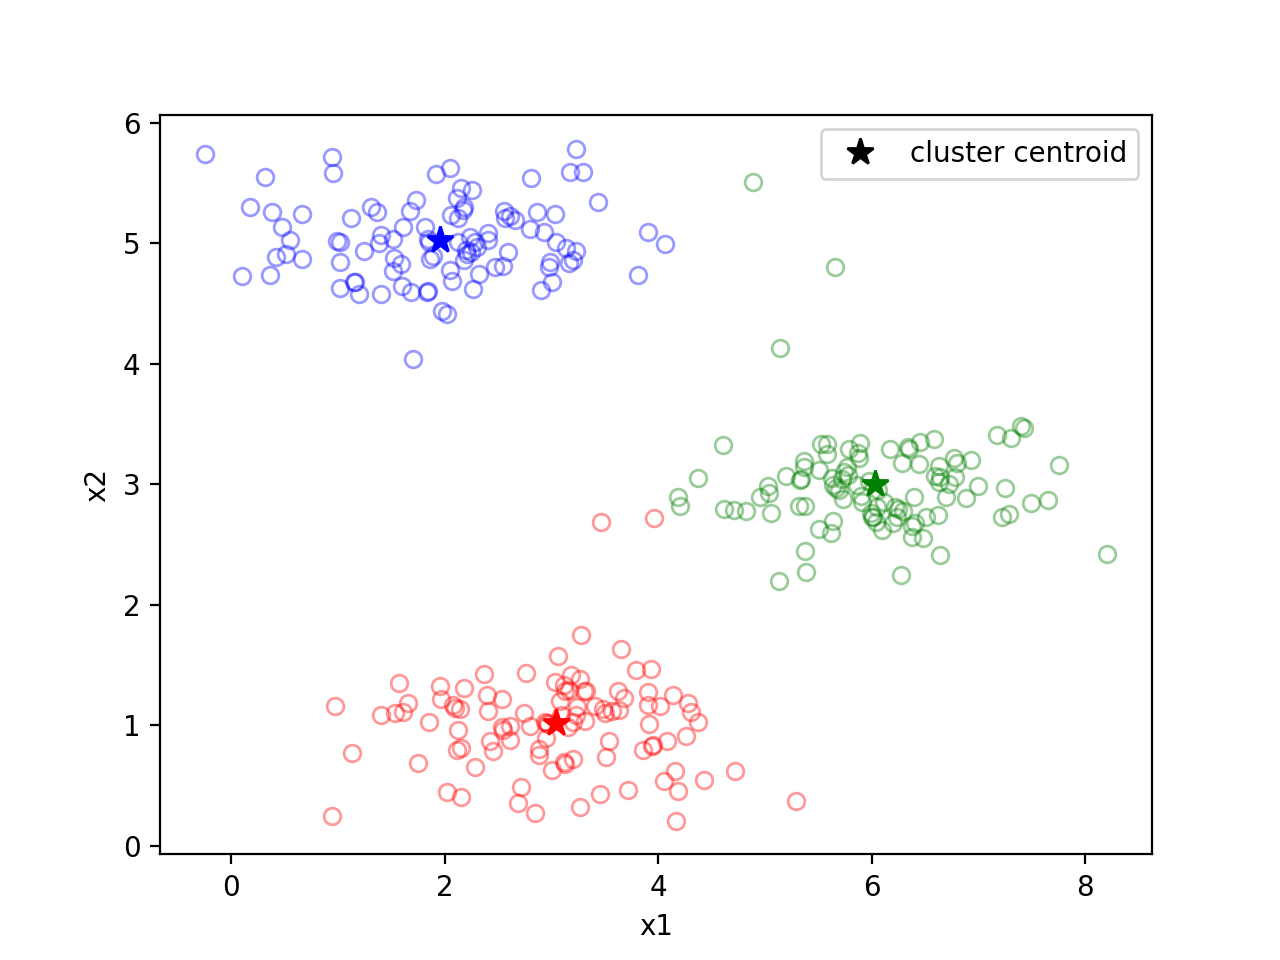
\includegraphics[width=0.5\linewidth]{figs/Chap_11_Figure_1.png}
\end{figure}


\paragraph{图像压缩}

图像是有若干像素组成的，每个像素存放 $3$ 个字节的信息代表其 $\text{RGB}$ 颜色，一张图片可能含有成百上千种颜色，如果我们只用 $16$ 种颜色表示它，那么我们只需要在对应像素位置存放一个 $4$ 位二进制数表示是第几种颜色，这样就把图像压缩到了原来的 $\frac{1}{6}$ 大小。

现在我们用 $\textbf{K-means}$ 算法去得到这 $16$ 种颜色。

我们使用的图像含有 $128\times128$ 个像素，可以处理为 $(128\times128,3)$ 的二维数组，每一行就是一个像素，包含 $3$ 个值，即 $\text{RGB}$. 这就是我们的输入数据。原图如下：

\begin{figure}[H]
    \centering
    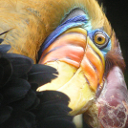
\includegraphics[width=0.3\linewidth]{figs/Chap_11_bird_small.png}
\end{figure}


\begin{lstlisting}[language=Python]
import numpy as np
from PIL import Image

def readin():
	data = np.array(Image.open('bird_small.png'))
	data = data.reshape((128*128, 3))
	return data

def J(X, cluster, centroid):
	res = 0
	for i in range(X.shape[0]):
		res += np.dot(X[i]-centroid[cluster[i]], X[i]-centroid[cluster[i]])
	return res

def K_means(K, X, iteration=100):
	(m, n) = X.shape
	bestCluster, bestCentroid, bestJ = np.empty(m), np.empty((K, n)), np.inf
	for iter in range(iteration):
		centroid = X[np.random.randint(0, m, K)]
		cluster = np.empty(m, dtype='int')
		while True:
			ncentroid = np.zeros((K, n))
			cnt = np.zeros(K)
			for i in range(m):
				cluster[i] = np.argmin(np.sum((X[i]-centroid)**2, axis=1))
				ncentroid[cluster[i]] += X[i]
				cnt[cluster[i]] += 1
			ncentroid[cnt!=0] /= cnt[cnt!=0][:, np.newaxis]
			ncentroid[cnt==0] = X[np.random.randint(0, m, len(cnt[cnt==0]))]
			if (centroid == ncentroid).all():
				break
			centroid = ncentroid.copy()
		cost = J(X, cluster, centroid)
		if cost < bestJ:
			bestCluster, bestCentroid, bestJ = cluster.copy(), centroid.copy(), cost.copy()
	return bestCluster, bestCentroid

X = readin()
cl, ce = K_means(16, X, iteration=20)

comImg = np.empty((128*128, 3), dtype='uint8')
for i in range(128*128):
	comImg[i] = np.floor(ce[cl[i]])
comImg = comImg.reshape((128, 128, 3))
im = Image.fromarray(comImg)
im.save('bird_compression.png')
\end{lstlisting}

得到的压缩结果如下：

\begin{figure}[H]
    \centering
    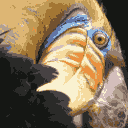
\includegraphics[width=0.3\linewidth]{figs/Chap_11_bird_compression.png}
\end{figure}
 \newpage
\section{主成分分析}
\label{sec:chapter12}

\subsection{数据降维}

我们的数据特征常常包含众多维度，但它们中的有些维度其实没有存在的必要。最极端的情况就是某一维度是其他若干维度的线性组合，那么这一维度就完全可以丢掉；但现实不会这么精准，如果某一维度是其他若干维度的线性组合加上微小的扰动，我们其实也可以将其丢掉。这就是数据降维。

\begin{figure}[H]
    \centering
    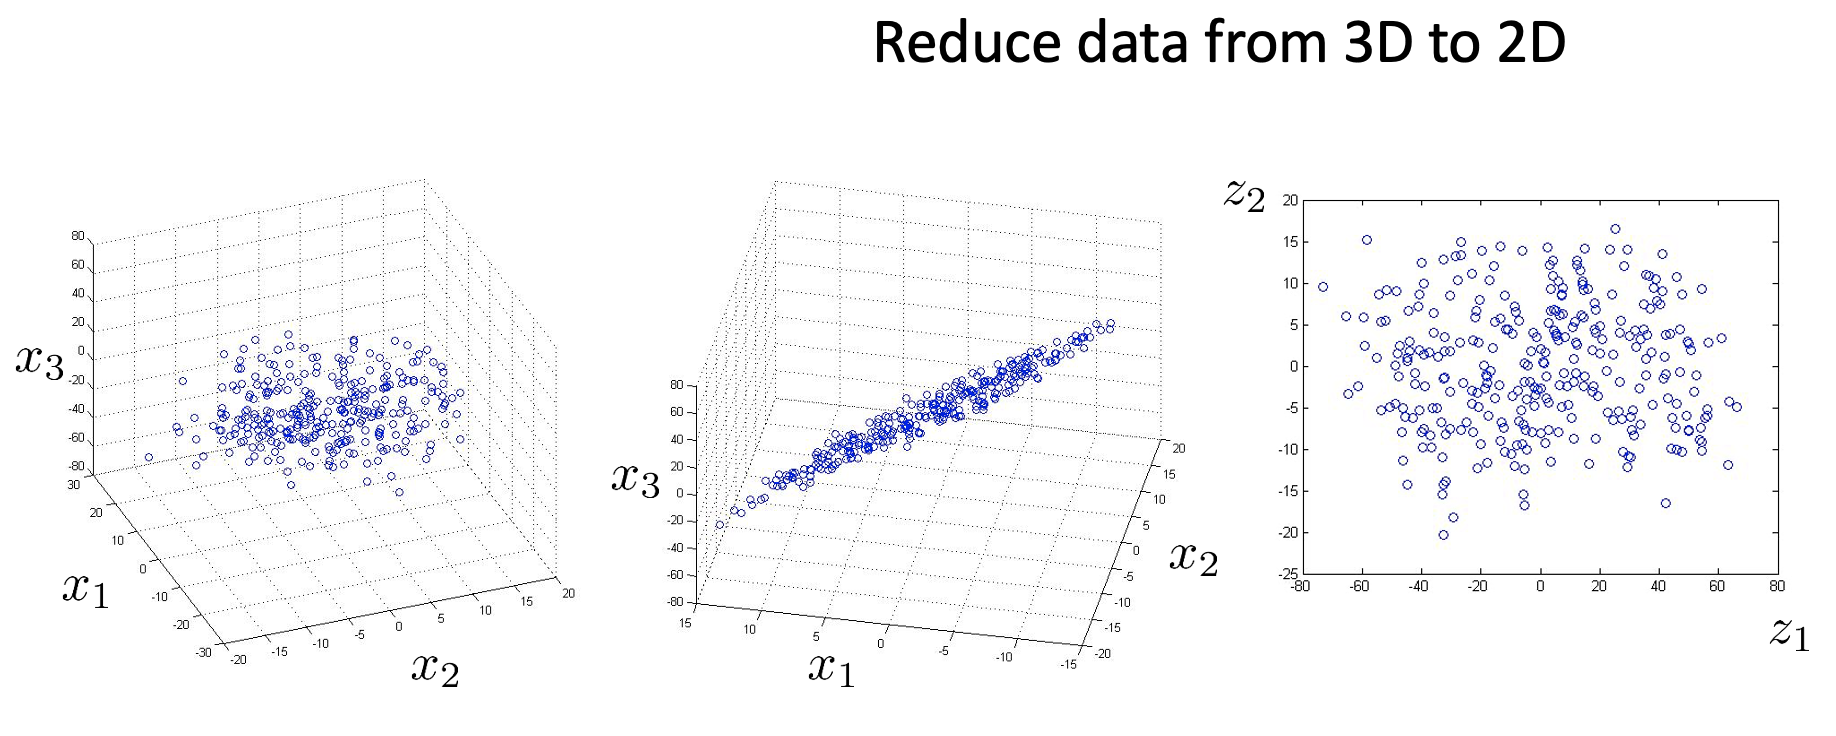
\includegraphics[width=\linewidth]{figs/Chap_12_data_compression.png}
\end{figure}

数据降维有众多算法可以完成，主成分分析即是其中之一。


\subsection{主成分分析}

主成分分析（Principal Component Analysis）的基本思想是：假设原始数据的特征有 $n$ 维，我们想将其缩减到 $k$ 维，那么我们只需要在原来的 $n$ 维空间中找到一个 $k$ 维的子空间，使得所有数据到这个子空间的距离平方和最小；此时，原数据在这个子空间上的投影就是我们新的 $k$ 维的数据。

\paragraph{数学推导}

为方便，我们首先将数据中心化，即使得数据的平均值在原点处。<u>一个获得所需要的 $k$ 维子空间的简单方式是：找到一个合适的 $n$ 维空间，直接选取前 $k$ 维作为子空间</u>。具体而言，对于一个数据点 $x=\begin{bmatrix}x_1\\x_2\\\vdots\\x_n\end{bmatrix}\in\mathbb R^n$，设我们要找的 $n$ 维空间的规范正交基为 $u_1,u_2,\ldots,u_n$，则 $x$ 在其中的新坐标为：
\[
y_j=x\cdot u_j=x_1u_{j1}+x_2u_{j2}+\cdots+x_nu_{jn}
\]
它到前 $k$ 维形成的子空间（即以 $u_1,u_2,\ldots,u_k$ 为基底的子空间）的距离之平方为：
\[
{y_{k+1}}^2+{y_{k+2}}^2+\cdots+{y_n}^2
\]
假设我们有 $m$ 个数据 $x^{(1)},x^{(2)},\ldots,x^{(m)}$，于是我们的优化目标为：
\[
\min \sum_{i=1}^m {y^{(i)}_{k+1}}^2+{y^{(i)}_{k+2}}^2+\cdots+{y^{(i)}_{n}}^2
\]
又由于在不同的基下 ${||x||}^2$ 都是一个定值，于是最小化上述距离等价于：
\[
\max \sum_{i=1}^m{y^{(i)}_1}^2+{y^{(i)}_2}^2+\cdots+{y^{(i)}_k}^2
\]
其充分条件为：
\[
\max \sum_{i=1}^m {y_r^{(i)}}^2,\quad r=1,2,\ldots,k
\]
这就是我们要解决的问题。

由于
\begin{align*}
\sum_{i=1}^m{y^{(i)}_r}^2&=\sum_{i=1}^m(x^{(i)}\cdot u_r)^2\\
&=\sum_{i=1}^m\left(u_r^Tx^{(i)}\right)\left({x^{(i)}}^Tu_r\right)\\
&=u_r^T\left(\sum_{i=1}^mx^{(i)}{x^{(i)}}^T\right) u_r
\end{align*}
这是一个正定二次型，$\sum\limits_{i=1}^mx^{(i)}{x^{(i)}}^T$ 是一个正定矩阵，可以进行奇异值分解：
\[
\sum_{i=1}^mx^{(i)}{x^{(i)}}^T=U\Sigma U^T
\]
其中，$U$ 是正交矩阵，$\Sigma$ 是对角矩阵 $\begin{bmatrix}\sigma_1&\cdots&0\\\vdots&\ddots&\vdots\\0&\cdots&\sigma_n\end{bmatrix}$，$\sigma_1,\ldots,\sigma_n$ 是奇异值，$\sigma_1>\cdots>\sigma_n$. 

令 $v_r=U^Tu_r$，由于 $U$ 正交，所以 $v_r$ 也是单位向量，代回得到：
\begin{align*}
\sum_{i=1}^m{y^{(i)}_r}^2&=u_r^TU\Sigma U^Tu_r\\
&=(U^T u_r)^T\Sigma(U^Tu_r)\\
&=v_r^T\Sigma v_r\\
&=\sigma_1v_{r1}^2+\sigma_2v_{r2}^2+\cdots+\sigma_nv_{rn}^2
\end{align*}
所以我们的优化目标变成了：
\begin{align*}
&\max\sum_{i=1}^n\sigma_iv_{ri}^2\\
&\text{s.t.}\begin{cases}\sum\limits_{i=1}^nv_{ri}^2=1\\\sigma_1>\cdots>\sigma_n\end{cases}
\end{align*}
很显然，它的解是：$v_{r1}=1,v_{r2}=\cdots=v_{rn}=0$，即 $v_r=\begin{bmatrix}1\\0\\\vdots\\0\end{bmatrix}$。又由于 $u_r=Uv_r$，<u>所以我们要找的 $n$ 维空间的各个基向量就是矩阵 $\sum\limits_{i=1}^mx^{(i)}{x^{(i)}}^T$ 的各个奇异值对应的奇异向量</u>，我们要降维到的 $k$ 维子空间的各个基向量就是前 $k$ 个奇异向量，对原来的数据进行基变换，就得到了降维后的数据。


\paragraph{步骤总结}

总结一下，主成分分析的推导过程稍显复杂，但是它的实现很简单，主要是以下步骤：

\begin{enumerate}
    \item 计算矩阵 $\sum\limits_{i=1}^mx^{(i)}{x^{(i)}}^T$；
    更简单的表达是：设矩阵 $X=\begin{bmatrix}{x^{(1)}}^T\\{x^{(2)}}^T\\\vdots\\{x^{(m)}}^T\end{bmatrix}$ 为数据集，那么计算矩阵 $X^TX$ 即可。
    \item 进行奇异值分解，得到奇异向量；
    \item 选取前 $k$ 个奇异向量作为降维后的空间的基向量，构成基变换矩阵 $C$；
    \item 对于原数据 $x$，取 $z=C^Tx$ 为其降维后的数据。
    更简单的表达是：取 $Z=XC$，则 $Z$ 是降维后的数据集。
\end{enumerate}


\paragraph{主成分数量的选择}

那么在实践中，我们到底选择多大的 $k$ 值比较好呢？对此，我们定义一个平均误差为：
\[
\frac{1}{m}\sum_{i=1}^m||x^{(i)}-x_\text{approx}^{(i)}||^2
\]
其中，$x_\text{approx}^{(i)}$ 表示数据 $x^{(i)}$ 在我们找到的 $k$ 维子空间上的投影。再定义一个总方差为：
\[
\frac{1}{m}\sum_{i=1}^m||x^{(i)}||^2
\]
则一般的，我们会选择最小的 $k$ 使得：
\[
\frac{\frac{1}{m}\sum\limits_{i=1}^m||x^{(i)}-x_\text{approx}^{(i)}||^2}{\frac{1}{m}\sum\limits_{i=1}^m||x^{(i)}||^2}\leqslant 0.01
\]
并称之为「$99\%$ 的方差得以保留」。

这个式子看起来并不好计算，但事实上，借助我们的奇异值，可以证明，对于给定的 $k$：
\[
\frac{\frac{1}{m}\sum\limits_{i=1}^m||x^{(i)}-x_\text{approx}^{(i)}||^2}{\frac{1}{m}\sum\limits_{i=1}^m||x^{(i)}||^2}=1-\frac{\sum\limits_{i=1}^k\sigma_k}{\sum\limits_{i=1}^n\sigma_i}
\]
这就好算了。


\subsection{代码实现}

\paragraph{二维压缩为一维}

二维平面上的原始数据：

\begin{figure}[H]
    \centering
    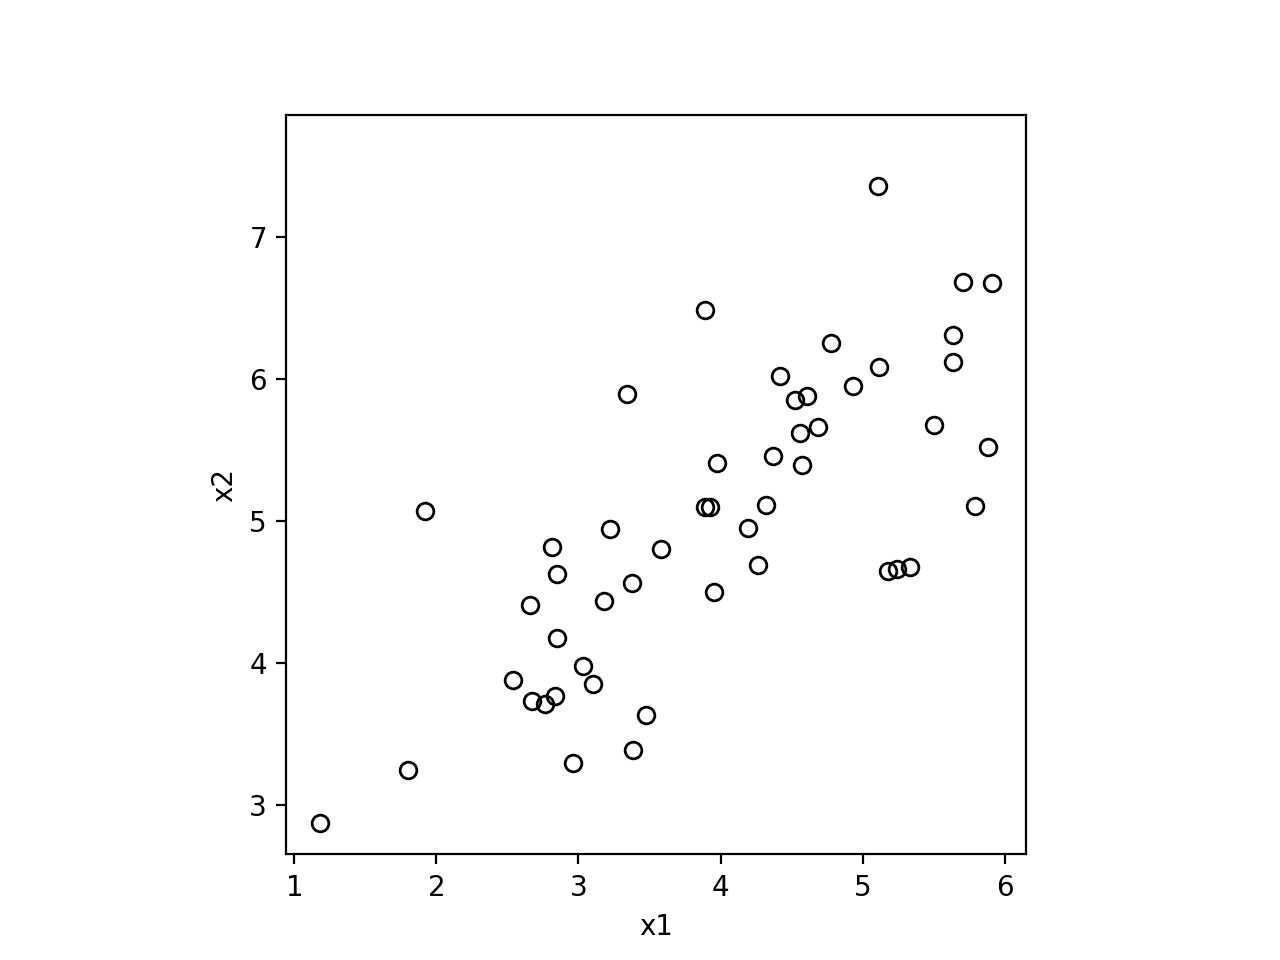
\includegraphics[width=0.5\linewidth]{figs/Chap_12_Figure_0.png}
\end{figure}

主成分分析代码：

\begin{lstlisting}[language=Python]
def PCA(X, dim = -1):
	"""
	X is the input data: (m, n)

	dim is the dimension after reduction
	if dim=-1, then the program select the smallest dim
	such that 99% of variance is retained
	
	return the data after reduction: (m, dim)
	and the data recovered from reduced data: (m, n)
	"""
	Xmean = np.empty((1, X.shape[1]))
	Xstd = np.empty((1, X.shape[1]))
	def normalization(X, k):
		global Xmean, Xstd
		if k == 1:
			Xmean = np.mean(X, axis=0)
			Xstd = np.std(X, axis=0, ddof=1)
			return (X - Xmean) / Xstd
		else:
			return X * Xstd + Xmean

	Xnorm = normalization(X, 1)
	u, s, v = np.linalg.svd(Xnorm.T @ Xnorm)
	if dim == -1:
		dim = 1
		while s[:dim].sum() / s.sum() < 0.99:
			dim += 1
	return Xnorm @ u[:, :dim], normalization(Xnorm @ u[:, :dim] @ u[:, :dim].T, 0)
\end{lstlisting}

得到映射的点：

\begin{figure}[H]
    \centering
    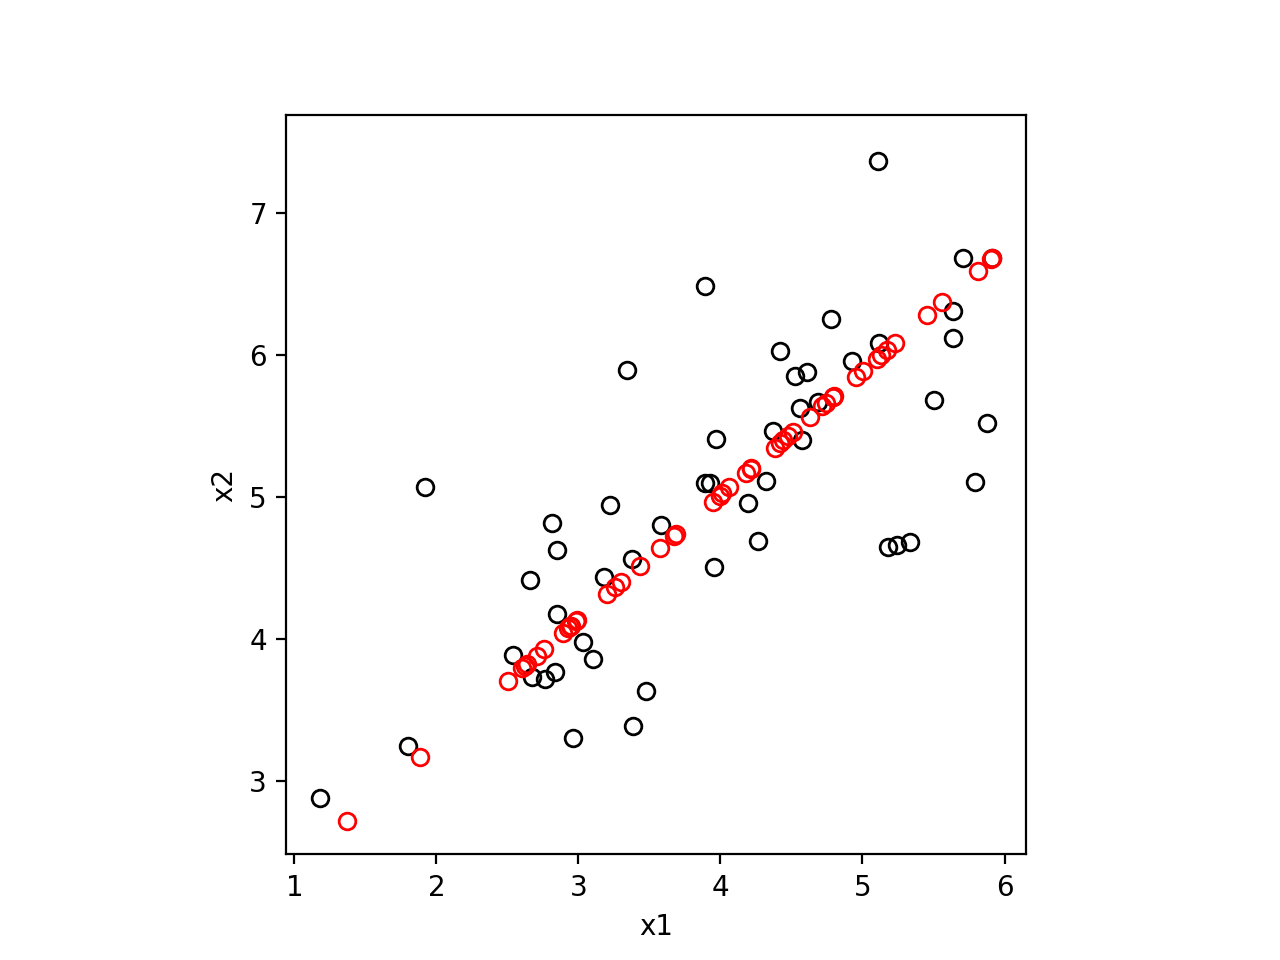
\includegraphics[width=0.5\linewidth]{figs/Chap_12_Figure_1.png}
\end{figure}

\paragraph{人脸特征压缩}

我们给出了 $5000$ 张人脸照片，每张照片含有 $32\times32$ 的灰度像素，形成维度为 $1024$ 的向量作为其特征。前 $100$ 张照片如图所示：

\begin{figure}[H]
    \centering
    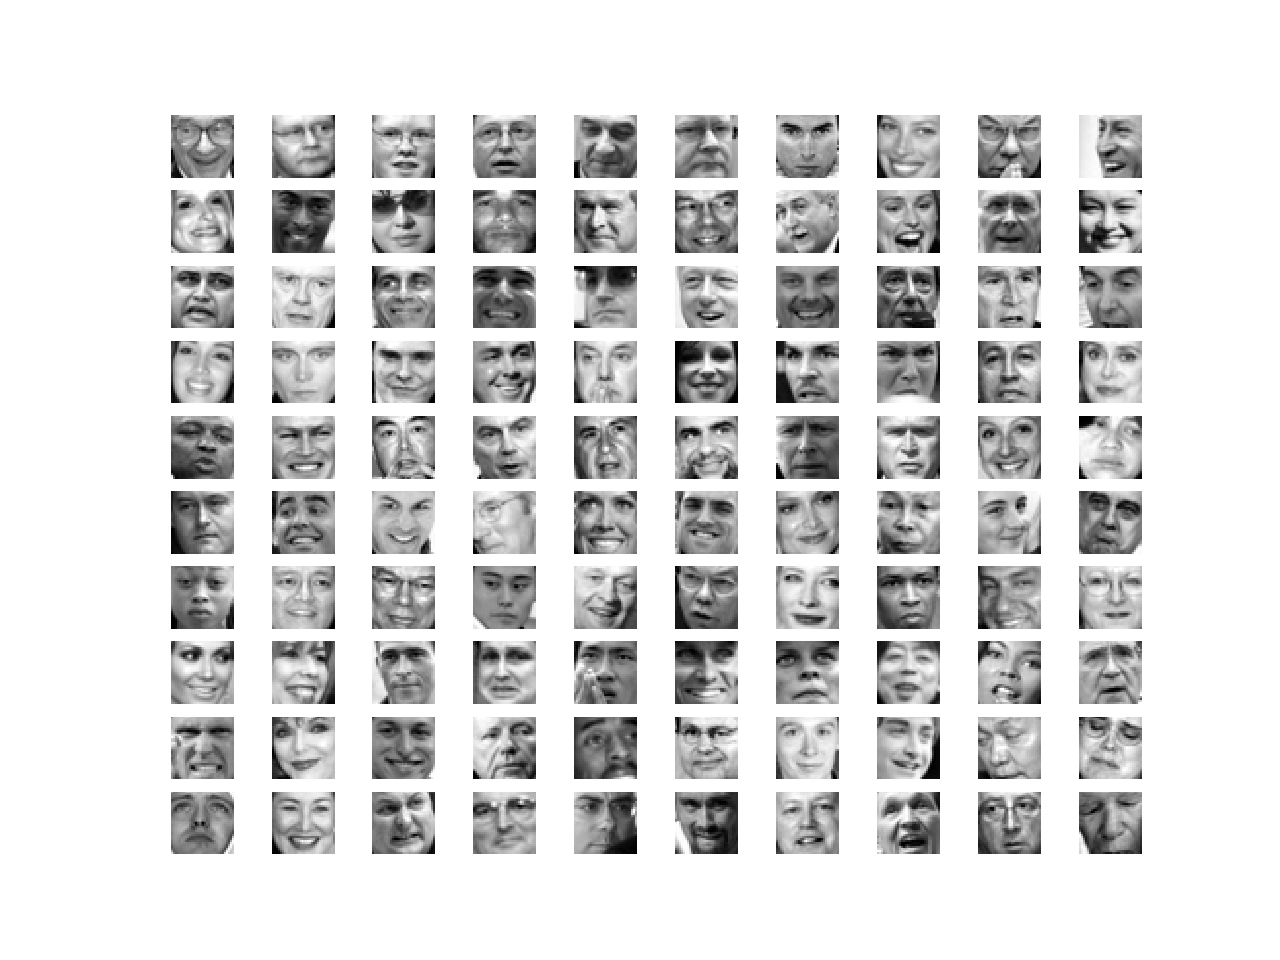
\includegraphics[width=\linewidth]{figs/Chap_12_Figure_2.png}
\end{figure}

现在将其压缩为 $\text{dim}={36,100}$ 维的数据，恢复后结果如下：

\begin{figure}[H]
    \centering
    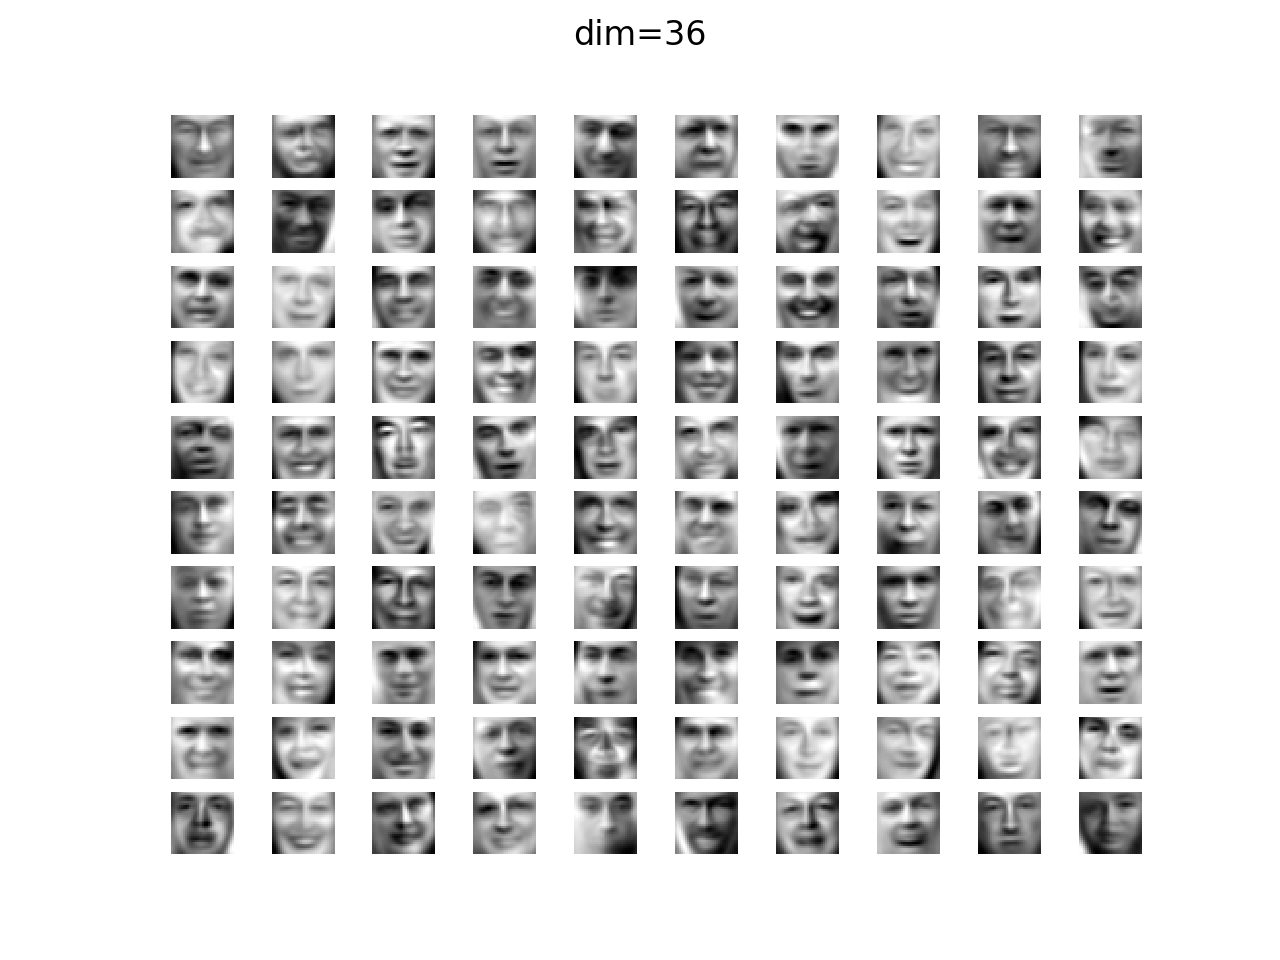
\includegraphics[width=\linewidth]{figs/Chap_12_Figure_dim=36.png}
\end{figure}

\begin{figure}[H]
    \centering
    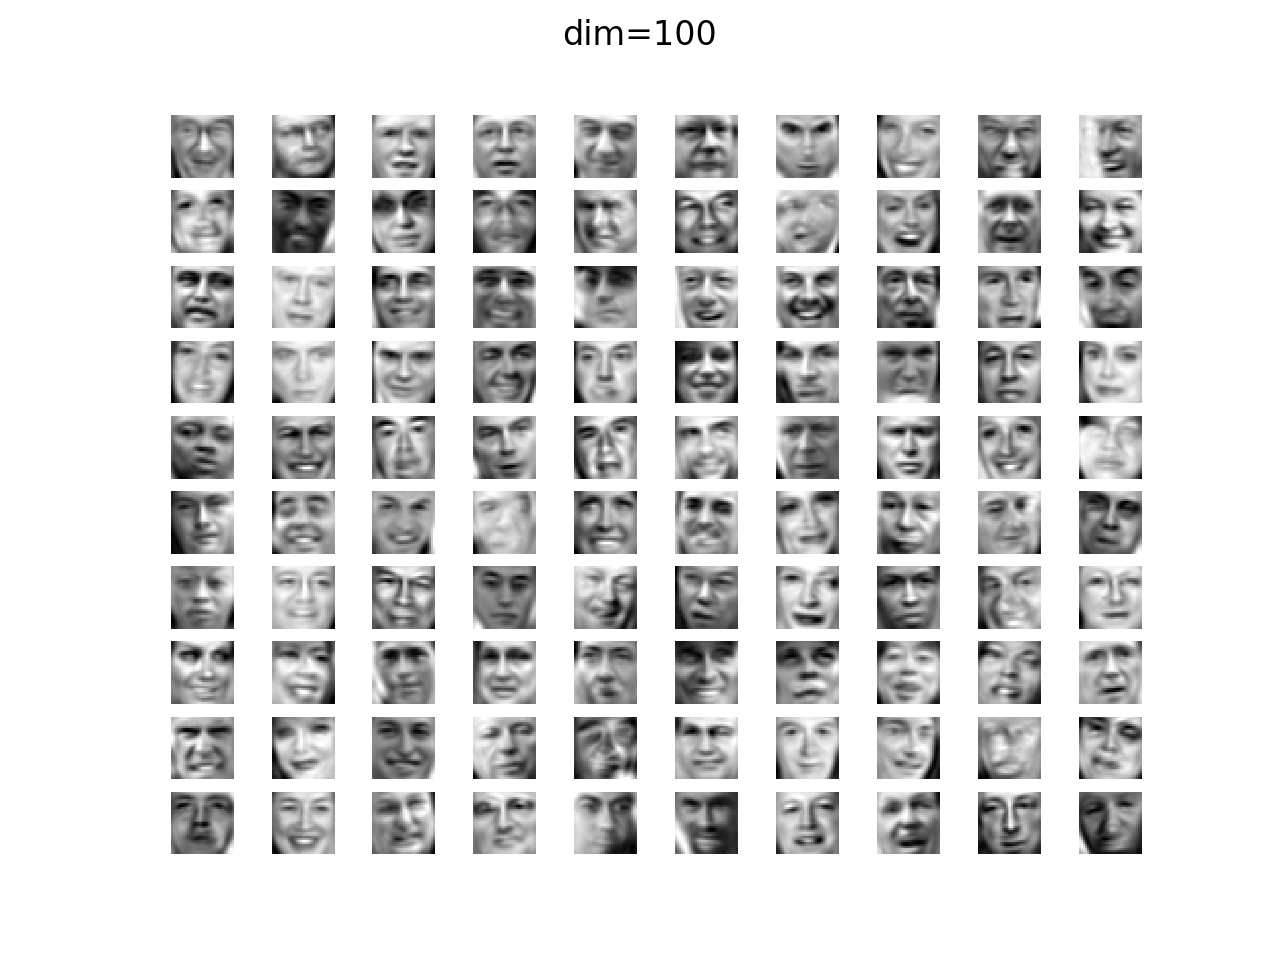
\includegraphics[width=\linewidth]{figs/Chap_12_Figure_dim=100.png}
\end{figure}
 \newpage
\section{异常检测}
\label{sec:chapter13}

\subsection{多元正态分布}

多元正态分布的概率密度函数为：
\[
p(x;\mu,\Sigma)=\frac{1}{(2\pi)^{n/2}|\Sigma|^{1/2}}\exp\left(-\frac{1}{2}(x-\mu)^T\Sigma^{-1}(x-\mu)\right)
\]
其中，$x\in\mathbb R^n$ 是 $n$ 维随机变量，$\mu\in\mathbb R^n$ 是 $x$ 的均值，$\Sigma\in\mathbb R^{n\times n}$ 是协方差矩阵。均值决定分布的中心位置，协方差矩阵则描述各维度的变化范围以及不同维度之间的相关关系。

特别地，当 $x$ 的各个维度不相关、协方差矩阵为对角矩阵时，联合概率密度可以分解为各分量概率密度的乘积，即：
\[
p(x;\mu,\Sigma)=\prod_{i=1}^np(x_i;\mu_i,\sigma_i^2)
\]


\subsection{异常检测}

异常检测的基本思想是先利用正常样本估计数据通常出现的区域，再将概率很低的新样本视为异常。设正常数据集为 $\{x^{(1)},x^{(2)},\ldots,x^{(m)}\}$，可以使用样本均值和协方差矩阵构建多元正态分布：
\begin{gather*}
\mu=\frac{1}{m}\sum\limits_{i=1}^mx^{(i)}\\
\Sigma=\frac{1}{m}\sum\limits_{i=1}^m(x^{(i)}-\mu)(x^{(i)}-\mu)^T\\
p(x;\mu,\Sigma)=\frac{1}{(2\pi)^{n/2}|\Sigma|^{1/2}}\exp\left(-\frac{1}{2}(x-\mu)^T\Sigma^{-1}(x-\mu)\right)
\end{gather*}
如果不希望估计完整协方差矩阵，也可以进一步假设 $x$ 的各维度相互独立，分别拟合每一维的正态分布，再取各概率密度之积：
\[
p(x;\mu,\Sigma)=\prod_{i=1}^np(x_i;\mu_i,\sigma_i^2)
\]

\begin{note}
后者计算更快，且允许 $m<n$ 的情况；而前者在 $m<n$ 时 $\Sigma$ 不可逆。
\end{note}

模型建立后，对于待检测样本 $x$，计算其在所拟合分布下的概率密度。若 $p(x;\mu,\Sigma)$ 小于阈值 $\varepsilon$，说明该样本在正常数据中出现的可能性很低，因此将其判定为异常；否则判定为正常。

若部分数据带有是否异常的标注，可以将数据划分为训练集、验证集和测试集。训练集主要包含正常样本，用于估计 $\mu$ 和 $\Sigma$ 并建立概率模型；验证集同时包含正常与异常样本，用于比较不同阈值并选择 $\varepsilon$；测试集同样包含两类样本，但只用于最终评估。

\begin{note}
异常检测通常属于类别极不平衡的问题，正常样本远多于异常样本。此时即使把所有样本都预测为正常，也可能得到很高的准确率，因此准确率并不是合适的主要指标。应使用 $\text{precision},\text{recall},\text{F1}$ 等指标综合评估异常样本的识别效果。
\end{note}


\subsection{代码实现}

根据训练集构建的二元正态分布如下：

\begin{figure}[H]
    \centering
    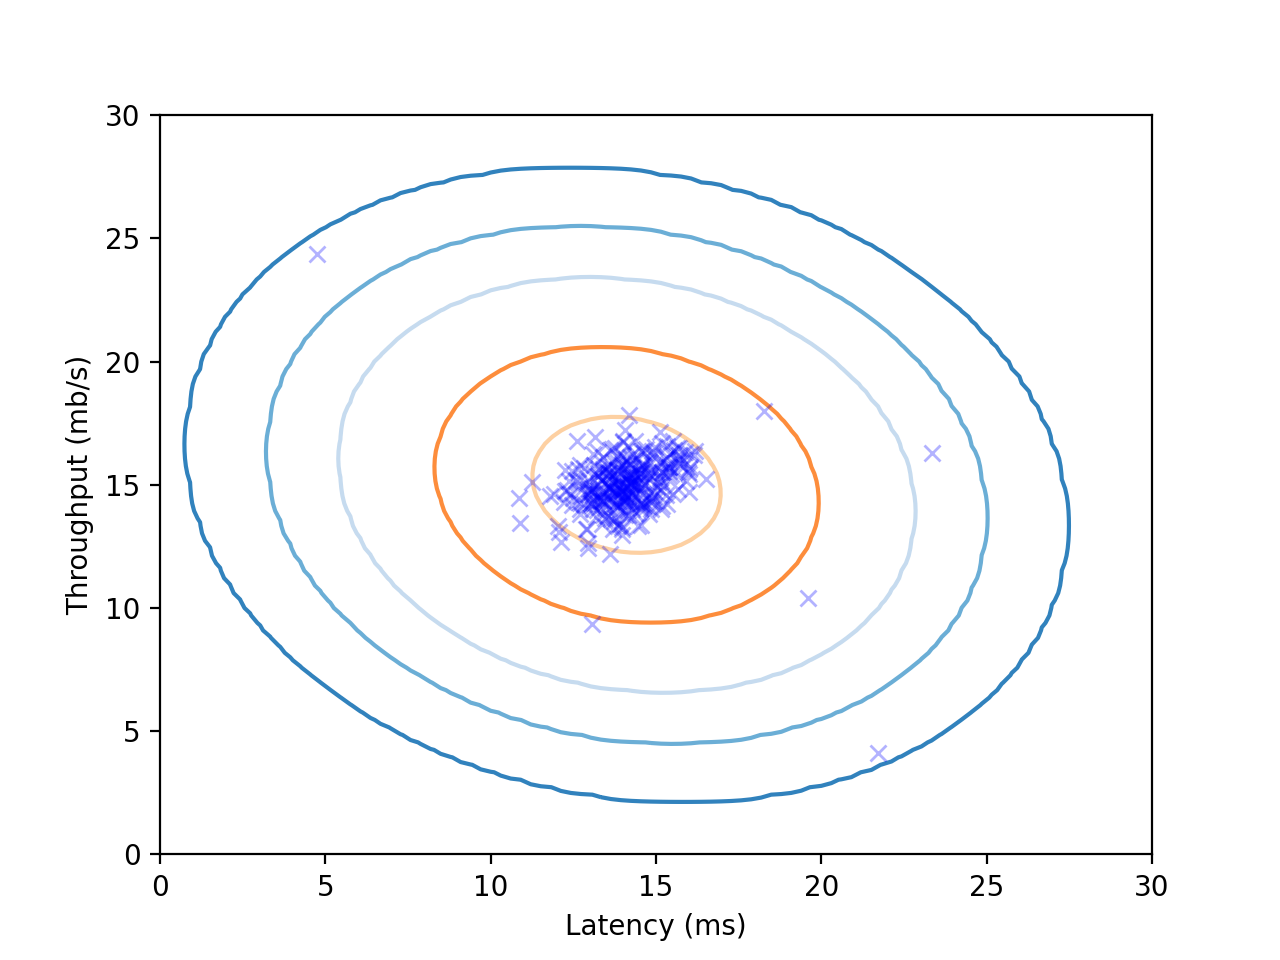
\includegraphics[width=0.5\linewidth]{figs/Chap_13_Figure_0.png}
\end{figure}

\begin{lstlisting}[language=Python]
Xmeans = X.mean(axis=0)
Xcov = ((X - Xmeans).T @ (X - Xmeans)) / X.shape[0]
normDist = multivariate_normal(mean=Xmeans, cov=Xcov)
\end{lstlisting}

依次尝试不同阈值，并根据验证集上的 $\text{F1}$ 选择最佳值。最终得到的最佳 $\varepsilon$ 约为 $2.72\times 10^{-5}$，此时测试集上的 $\text{F1}$ 约为 $0.75$. 

\begin{figure}[H]
    \centering
    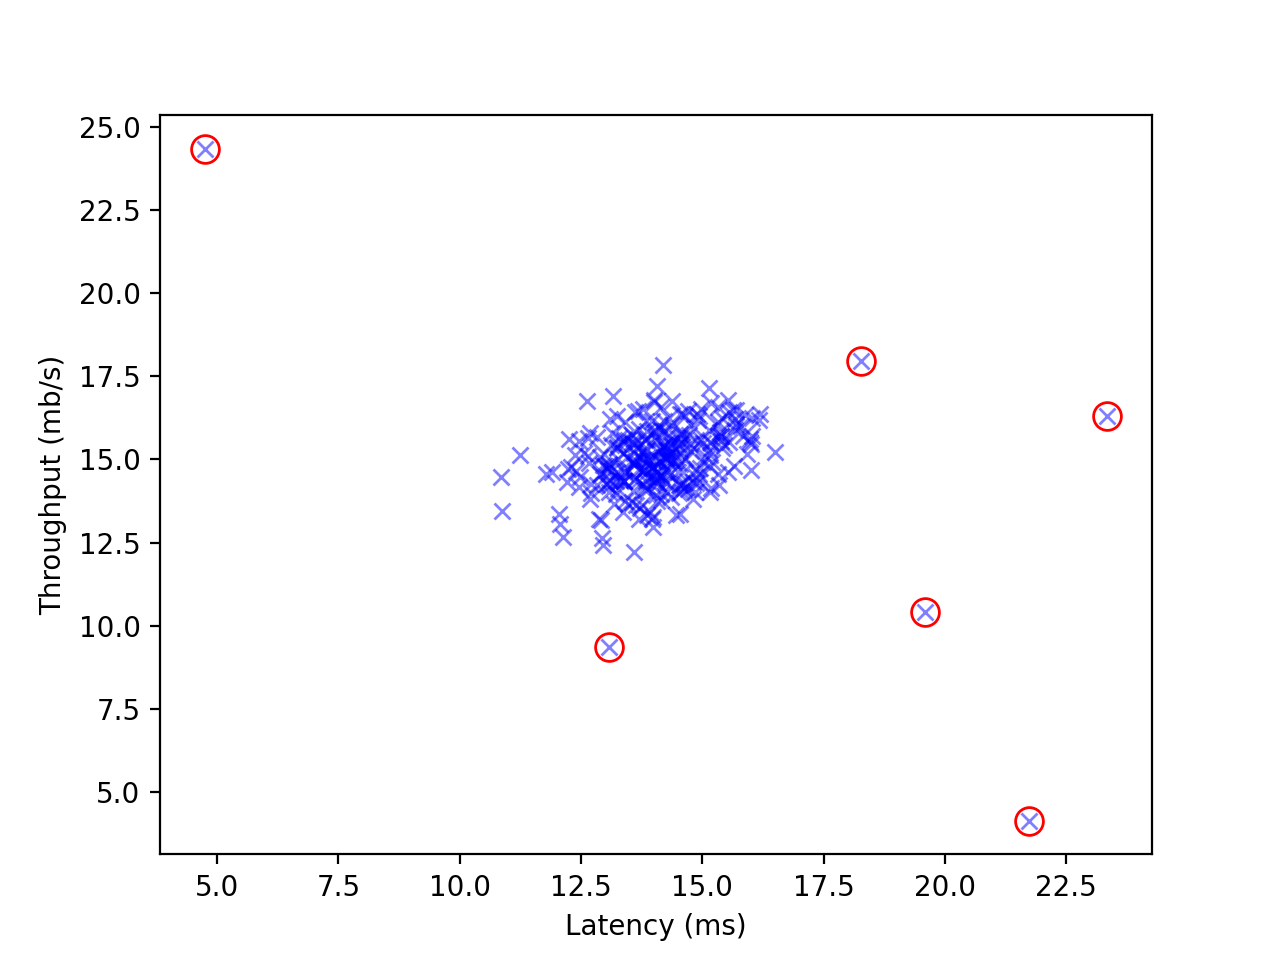
\includegraphics[width=0.5\linewidth]{figs/Chap_13_Figure_1.png}
\end{figure}
 \newpage
\section{推荐系统}
\label{sec:chapter14}

\subsection{基于内容的推荐算法}

以向用户推荐电影为例。假设已经为每部电影构建了特征向量，例如不同类型或题材所占的程度，并且已知每个用户对部分电影的评分。对于某个用户，可以将电影特征作为自变量 $x$、该用户的评分作为因变量 $y$，从而为每个用户建立一个独立的\textbf{线性回归}模型。

设共有 $n_u$ 个用户和 $n_m$ 部电影，第 $i$ 部电影的特征向量为 $x^{(i)}\in\mathbb R^{n+1}$（包含偏置项）。$r(i,j)$ 表示用户 $j$ 是否评价了电影 $i$；若已经评分，则对应分数记为 $y^{(i,j)}$. 对于用户 $j$，只使用他已经评价过的电影训练参数 $\theta^{(j)}$，优化目标为：
\[
\min_{\theta^{(j)}}~~\frac{1}{2}\sum_{i:r(i,j)=1}\left((\theta^{(j)})^Tx^{(i)}-y^{(i,j)}\right)^2+\frac{\lambda}{2}\sum_{k=1}^{n}(\theta_k^{(j)})^2
\]
每个用户的线性回归在形式上相互独立，但可以把所有用户的目标函数相加，统一训练全部参数：
\[
J(\theta^{(1)},\ldots,\theta^{(n_u)}):=\frac{1}{2}\sum_{j=1}^{n_u}\sum_{i:r(i,j)=1}\left((\theta^{(j)})^Tx^{(i)}-y^{(i,j)}\right)^2+\frac{\lambda}{2}\sum_{j=1}^{n_u}\sum_{k=1}^{n}(\theta_k^{(j)})^2
\]
为了使用梯度下降等方法优化，所需的偏导数为：
\[
\frac{\partial J}{\partial\theta^{(j)}_k}=\sum_{i:r(i,j)=1}\left((\theta^{(j)})^Tx^{(i)}-y^{(i,j)}\right)\theta^{(j)}_k+\lambda\theta_k^{(j)}[k>0]
\]
训练完成后，对于特征向量为 $x$ 的任意电影，用户 $j$ 的预测评分为 $(\theta^{(j)})^Tx$. 可以据此对用户尚未评价的电影排序，并推荐预测评分较高的项目。

基于内容的推荐算法有一个明显限制：必须预先知道每部电影的特征向量。然而，哪些特征最能解释用户偏好往往难以确定，人工标注大量电影也需要较高成本。为避免依赖显式内容特征，可以使用协同过滤，从用户评分数据中同时学习电影和用户的表示。


\subsection{协同过滤算法}

\paragraph{初始版本}

现在假设电影特征未知，但可以通过询问用户等方式获得用户参数 $\theta^{(j)}$，例如用户对不同类型电影的偏好。这样便可以反过来把用户参数作为已知量，根据评分学习电影特征 $x^{(i)}$. 对于第 $i$ 部电影，只使用评价过该电影的用户，优化目标为：
\[
\min_{\theta^{(j)}}~~\frac{1}{2}\sum_{j:r(i,j)=1}\left((\theta^{(j)})^Tx^{(i)}-y^{(i,j)}\right)^2+\frac{\lambda}{2}\sum_{k=1}^{n}(x_k^{(i)})^2
\]
与前面按用户训练参数类似，各电影特征的优化也相互独立，可以将它们的目标相加后统一写为：
\[
J(x^{(1)},\ldots,x^{(n_m)}):=\frac{1}{2}\sum_{i=1}^{n_m}\sum_{j:r(i,j)=1}\left((\theta^{(j)})^Tx^{(i)}-y^{(i,j)}\right)^2+\frac{\lambda}{2}\sum_{i=1}^{n_m}\sum_{k=1}^{n}(x_k^{(i)})^2
\]
为了优化电影特征，所需的偏导数为：
\[
\frac{\partial J}{\partial x^{(i)}_k}=\sum_{j:r(i,j)=1}\left((\theta^{(j)})^Tx^{(i)}-y^{(i,j)}\right)\theta^{(i)}_k+\lambda x_k^{(i)}[k>0]
\]

总结而言，已知 $\theta^{(j)}$ 时可以学习 $x^{(i)}$，已知 $x^{(i)}$ 时也可以学习 $\theta^{(j)}$. 因此，可以先随机初始化一组用户参数，用它们学习所有电影特征；再固定新得到的电影特征，重新学习用户参数；随后继续使用新的用户参数更新电影特征。如此在两组参数之间\textbf{交替优化}，直至电影特征和用户参数都趋于稳定，这构成了协同过滤算法的初始版本。


\paragraph{改进版本}

实际上，没有必要把两组参数拆开并手工反复交替训练。观察“固定用户参数学习电影特征”和“固定电影特征学习用户参数”这两个优化目标，可以发现它们的非正则化项完全相同，均为 $\sum_{(i,j):r(i,j)=1}\left((\theta^{(j)})^Tx^{(i)}-y^{(i,j)}\right)^2$. 因此，只需合并两边的正则化项，就可以把电影特征和用户参数放入同一个目标函数中同时优化：
\begin{gather*}
J(x^{(1)},\ldots,x^{(n_m)},\theta^{(1)},\ldots,\theta^{(n_u)})=\\\frac{1}{2}\sum_{(i,j):r(i,j)=1}\left((\theta^{(j)})^Tx^{(i)}-y^{(i)}\right)^2+\frac{\lambda}{2}\sum_{i=1}^{n_m}\sum_{k=1}^n(x^{(i)}_k)^2+\frac{\lambda}{2}\sum_{j=1}^{n_u}\sum_{k=1}^n(\theta^{(j)}_k)^2
\end{gather*}
值得注意的是，在改进版本中，特征由模型自动学习。由于电影特征和用户参数可以共同吸收整体偏移，模型中\textbf{无须额外加入偏置项}，因此 $x^{(i)}\in\mathbb R^n,\theta^{(j)}\in\mathbb R^n$.

上式的偏导数为：
\begin{align*}
&\frac{\partial J}{\partial\theta^{(j)}_k}=\sum_{i:r(i,j)=1}\left((\theta^{(j)})^Tx^{(i)}-y^{(i,j)}\right)\theta^{(j)}_k+\lambda\theta_k^{(j)}\\
&\frac{\partial J}{\partial x^{(i)}_k}=\sum_{j:r(i,j)=1}\left((\theta^{(j)})^Tx^{(i)}-y^{(i,j)}\right)x^{(i)}_k+\lambda x_k^{(i)}
\end{align*}
得到目标函数和梯度后，可以使用梯度下降或其他算法（如 LBFGS 等）进行优化。


\paragraph{向量化版本}

逐项遍历所有电影和用户会产生较大开销。为提高代码运行效率，需要将协同过滤算法写成矩阵形式并进行并行计算。

构造评分矩阵 $Y:=\begin{bmatrix}y^{(i,j)}\end{bmatrix}\in\mathbb R^{n_m\times n_u}$，其第 $i$ 行第 $j$ 列表示用户 $j$ 对电影 $i$ 的评分；构造电影特征矩阵 $X:=\begin{bmatrix}(x^{(1)})^T\\ \vdots\\ (x^{(n_m)})^T\end{bmatrix}\in\mathbb R^{n_m\times n}$，其第 $i$ 行是电影 $i$ 的特征向量；再构造用户参数矩阵 $\Theta:=\begin{bmatrix}(\theta^{(1)})^T\\ \vdots\\ (\theta^{(n_u)})^T\end{bmatrix}\in\mathbb R^{n_u\times n}$，其第 $j$ 行是用户 $j$ 的参数向量。由此，所有用户对所有电影的预测评分可以一次写成矩阵：
\[
X\Theta^T\in\mathbb R^{n_m\times n_u}
\]
利用 \texttt{numpy} 的语法可以简洁地实现代价函数及其梯度的向量化计算，详见代码。


\subsection{代码实现}

\begin{lstlisting}[language=Python]
import numpy as np
from scipy.io import loadmat
from scipy.optimize import minimize

def J(Y, R, X, Theta, lamb):
	return 0.5 * (np.sum(((X @ Theta.T - Y) * R) ** 2) + \
		lamb * np.sum(X ** 2) + lamb * np.sum(Theta ** 2))

def partJ(Y, R, X, Theta, lamb):
	return np.concatenate((
		( ((X @ Theta.T - Y) * R) @ Theta + lamb * X ).flatten(), 
		( ((X @ Theta.T - Y) * R).T @ X + lamb * Theta ).flatten()
	))

def train(Y, R, lamb, n):
	(n_m, n_u) = Y.shape
	xt = np.empty(n*n_m+n*n_u)
	return minimize(fun = lambda xt, Y, R, lamb : J(Y, R, xt[:n*n_m].reshape((n_m, n)), \
													xt[n*n_m:].reshape((n_u, n)), lamb), 
					x0 = np.random.randn(n*n_m+n*n_u), 
					args = (Y, R, lamb), 
					method = 'TNC', 
					jac = lambda xt, Y, R, lamb: partJ(Y, R, xt[:n*n_m].reshape((n_m, n)), \
													xt[n*n_m:].reshape((n_u, n)), lamb)
					)

def predict(Y, R, xt, n):
	(n_m, n_u) = Y.shape
	X, Theta = xt[:n*n_m].reshape((n_m, n)), xt[n*n_m:].reshape((n_u, n))
	return X @ Theta.T

data = loadmat('ex8_movies.mat')
Y = data['Y']
R = data['R']
Ymean = Y.mean(axis=1, keepdims=True)
res = train(Y-Ymean, R, lamb=1, n=50)
print(res)
np.save('xt.npy', res.x)
xt = res.x
\end{lstlisting}

优化结果为：

\begin{lstlisting}
     fun: 11078.825074101991
     jac: array([ 4.75273039e-07, -8.33595791e-07, -4.85091646e-07, ...,
        9.67607422e-07,  3.80539749e-06,  1.86386969e-06])
 message: 'Converged (|f_n-f_(n-1)| ~= 0)'
    nfev: 14671
     nit: 463
  status: 1
 success: True
       x: array([ 0.30269431, -1.3577984 , -0.19821756, ...,  0.12718836,
       -0.40793964, -0.60753772])
\end{lstlisting}

优化得到电影特征和用户参数后，先计算完整的预测评分矩阵，再从中选取第一个用户预测评分最高的 $10$ 部电影：

\begin{lstlisting}[language=Python]
xt = np.load('xt.npy')
pred = predict(Y, R, xt, n=50) + Ymean
movie_list = []
with open('movie_ids.txt', encoding='latin-1') as file:
	for line in file:
		movie_list.append(' '.join(line.strip().split(' ')[1: ]))
movie_list = np.array(movie_list)
idx = np.argsort(pred[:, 0])[::-1]
print('Top 10 movies for user 1:')
for movie in movie_list[idx][:10]:
	print(movie)
\end{lstlisting}

结果为：

\begin{lstlisting}
Top 10 movies for user 1:
Titanic (1997)
In the Name of the Father (1993)
Philadelphia (1993)
Duck Soup (1933)
Ice Storm, The (1997)
Saint, The (1997)
William Shakespeare's Romeo and Juliet (1996)
Boot, Das (1981)
People vs. Larry Flynt, The (1996)
Manhattan (1979)
\end{lstlisting}
 \newpage
\section{总结与使用 \texttt{scikit-learn}}
\label{sec:chapter15}

\subsection{总结}

吴恩达老师的机器学习系列课程到这里就结束了，$40$ 天里，我学到了许多有趣的、极具吸引力的机器学习知识，相信若干年后想起这段时光，仍然会感谢吴恩达老师带我入门了这个领域。

在这门课上，我们学习了以下内容：

\begin{itemize}
    \item 监督学习 Supervised learning
      \begin{itemize}
        \item 线性回归 Linear regression （第 \ref{sec:chapter1},\ref{sec:chapter2},\ref{sec:chapter3} 章）
        \item 逻辑回归 Logistic regression（第 \ref{sec:chapter4},\ref{sec:chapter5},\ref{sec:chapter6} 章）
        \item (BP)神经网络 Neural networks（第 \ref{sec:chapter7},\ref{sec:chapter8} 章）
        \item 支持向量机 Support vector machines（第 \ref{sec:chapter10} 章）
      \end{itemize}
    \item 无监督学习 Unsupervised learning
      \begin{itemize}
        \item K-Means（第 \ref{sec:chapter11} 章）
        \item 主成分分析 Principal component analysis（第 \ref{sec:chapter12} 章）
        \item 异常检测 Anomaly detection（第 \ref{sec:chapter13} 章）
      \end{itemize}
    \item 特殊应用/特殊专题
      \begin{itemize}
        \item 推荐系统 Recommender systems（协同过滤 Collaborative filtering）（第 \ref{sec:chapter14} 章）
        \item 大规模机器学习 Large scale machine learning
      \end{itemize}
    \item 建立机器学习模型时的一些建议
      \begin{itemize}
        \item 方差与偏差 Bias / variance（第 \ref{sec:chapter9} 章）
        \item 正则化 Regularization（第 \ref{sec:chapter5} 章）
        \item 对学习算法的评价：precision, recall, f1 score
        \item 学习曲线 Learning curves（第 \ref{sec:chapter9} 章）
        \item 误差分析 Error analysis
        \item 上界分析 Ceiling analysis
      \end{itemize}
\end{itemize}


\subsection{使用 \texttt{scikit-learn} 进行机器学习}

学习过程中的代码基本都是自己实现的，运行效率和使用容易程度上不敢恭维……现在清楚了原理之后，就可以放心大胆地调包了。

\paragraph{线性回归}

\begin{center}
\begin{lstlisting}[language=Python]
"""
class sklearn.linear_model.LinearRegression(*, fit_intercept=True, 
normalize=False, copy_X=True, n_jobs=None, positive=False)
"""

import numpy as np
import matplotlib.pyplot as plt
from sklearn.linear_model import LinearRegression

data = np.loadtxt('data/ex1data1.txt', delimiter=',')
y = data[:, -1]
X = data[:, :-1]

reg = LinearRegression(normalize=True)
reg.fit(X, y)
print(reg.score(X, y))

ax = plt.subplot(1, 1, 1)
ax.set_xlabel('x')
ax.set_ylabel('y')
ax.set_title('Linear Regression')
ax.plot(X.flatten(), y, 'x', color='red')
ax.plot(X, reg.predict(X))
plt.show()
\end{lstlisting}
\end{center}

\begin{figure}[H]
    \centering
    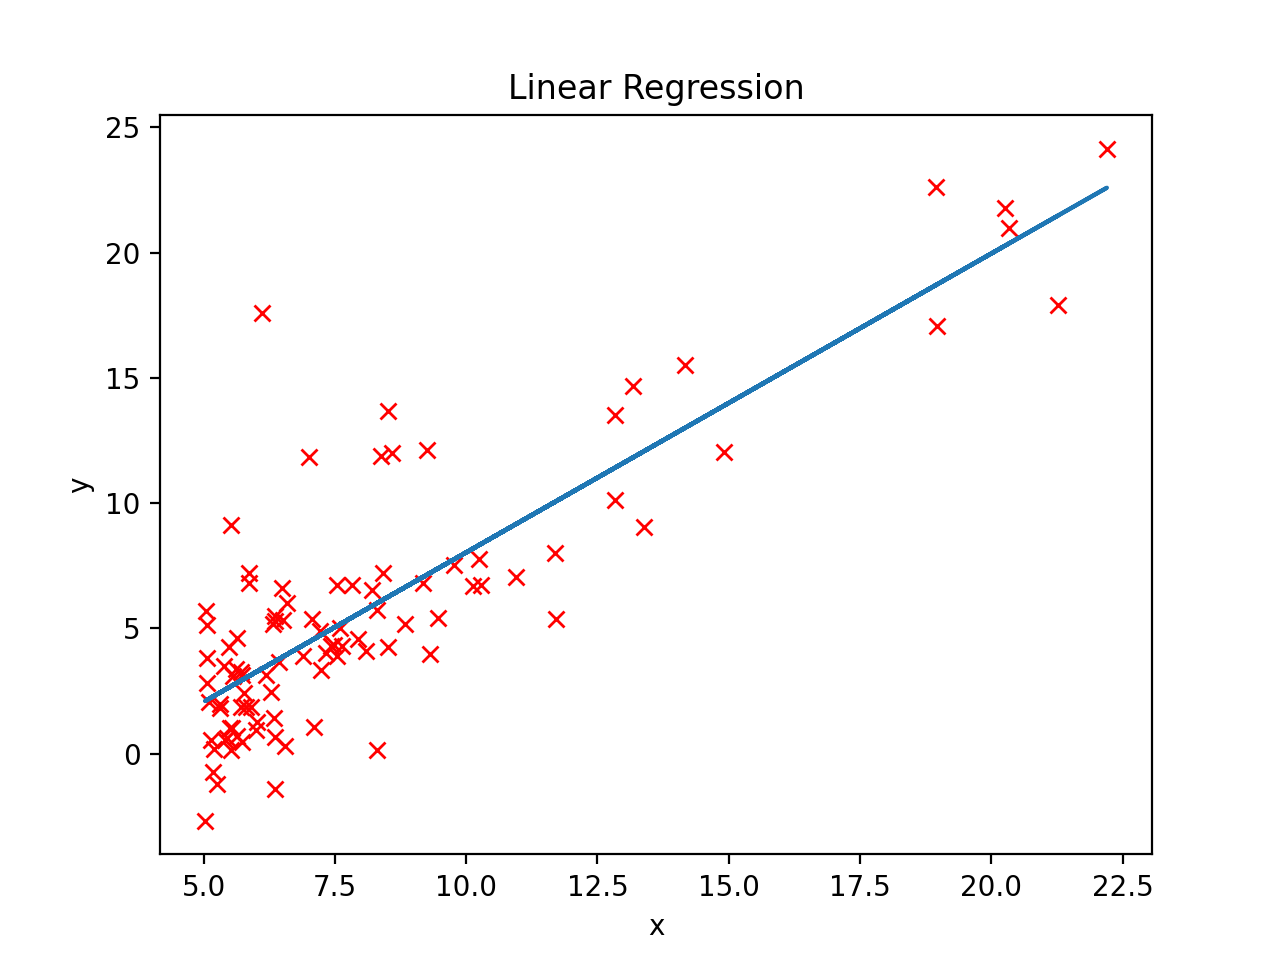
\includegraphics[width=0.5\linewidth]{figs/Chap_15_LinearRegression.png}
\end{figure}

\begin{lstlisting}[language=Python]
"""
class sklearn.linear_model.LinearRegression(*, fit_intercept=True, 
normalize=False, copy_X=True, n_jobs=None, positive=False)
"""

import numpy as np
import matplotlib.pyplot as plt
from sklearn.linear_model import LinearRegression

data = np.loadtxt('data/ex1data2.txt', delimiter=',')
y = data[:, -1]
X = data[:, :-1]

reg = LinearRegression(normalize=True)
reg.fit(X, y)
print(reg.score(X, y))
print(reg.predict(X))
\end{lstlisting}

\paragraph{逻辑回归}

\begin{center}
\begin{lstlisting}[language=Python]
"""
class sklearn.linear_model.LogisticRegression(penalty='l2', *, dual=False, 
tol=0.0001, C=1.0, fit_intercept=True, intercept_scaling=1, 
class_weight=None, random_state=None, solver='lbfgs', max_iter=100, 
multi_class='auto', verbose=0, warm_start=False, n_jobs=None, l1_ratio=None)
"""

import numpy as np
import matplotlib.pyplot as plt
from sklearn.linear_model import LogisticRegression

data = np.loadtxt('data/ex2data1.txt', delimiter=',')
y = data[:, -1]
X = data[:, :-1]

clf = LogisticRegression()
clf.fit(X, y)
print(clf.score(X, y))

ax = plt.subplot(1, 1, 1)
ax.set_xlabel('x1')
ax.set_ylabel('x2')
ax.set_title('Logistic Regression')
ax.plot(X[y==0][:, 0], X[y==0][:, 1], 'x', color='red')
ax.plot(X[y==1][:, 0], X[y==1][:, 1], 'o', color='blue', markerfacecolor='none')
x1, x2 = np.meshgrid(np.linspace(X[:, 0].min(), X[:, 0].max(), 100), 
	np.linspace(X[:, 1].min(), X[:, 1].max(), 100))
ax.contour(x1, x2, 
	clf.predict_proba(np.array([x1, x2]).\
	transpose(2, 1, 0).reshape((10000, 2)))[:, 0].reshape(100, 100), [0.5])
ax.axis('square')

plt.show()
\end{lstlisting}
\end{center}

\begin{figure}[H]
    \centering
    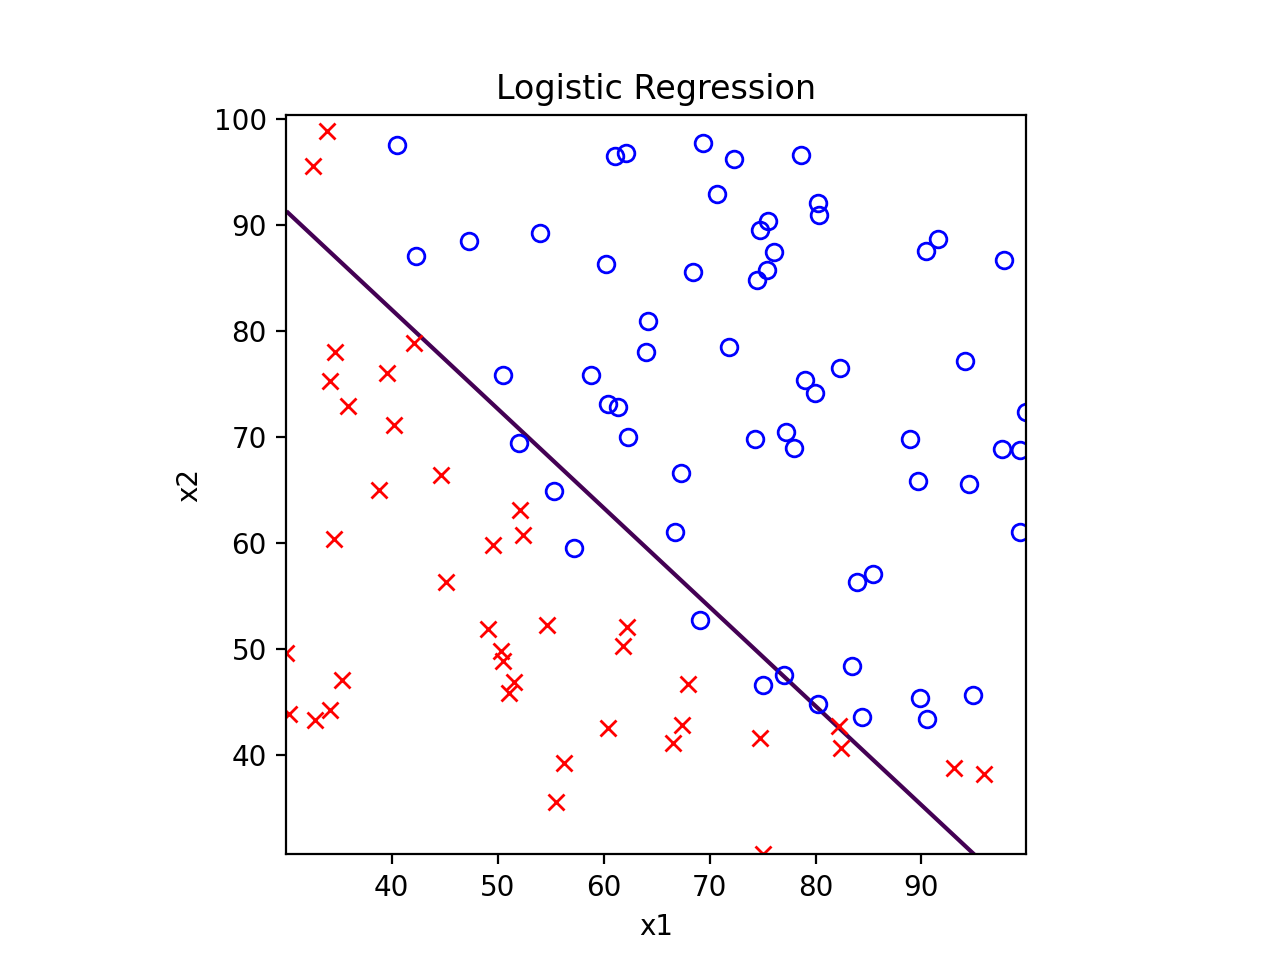
\includegraphics[width=0.5\linewidth]{figs/Chap_15_LogisticRegression.png}
\end{figure}

\begin{lstlisting}[language=Python]
"""
class sklearn.linear_model.LogisticRegression(penalty='l2', *, dual=False, 
tol=0.0001, C=1.0, fit_intercept=True, intercept_scaling=1, 
class_weight=None, random_state=None, solver='lbfgs', max_iter=100, 
multi_class='auto', verbose=0, warm_start=False, n_jobs=None, l1_ratio=None)

class sklearn.preprocessing.PolynomialFeatures(degree=2, *, 
interaction_only=False, include_bias=True, order='C')
"""

import numpy as np
import matplotlib.pyplot as plt
from sklearn.linear_model import LogisticRegression
from sklearn.linear_model import LogisticRegressionCV
from sklearn.preprocessing import PolynomialFeatures

data = np.loadtxt('data/ex2data2.txt', delimiter=',')
y = data[:, -1]
X = data[:, :-1]
poly = PolynomialFeatures(degree=5)
newX = poly.fit_transform(X)

fig, ax = plt.subplots(1, 4)
fig.suptitle('Logistic Regression')
Cs = [0.01, 1, 300, -1]
for i in range(4):
	C = Cs[i]
	if i < 3:
		clf = LogisticRegression(C=C, max_iter=1000)
	else:
		clf = LogisticRegressionCV(max_iter=1000)
	clf.fit(newX, y)
	print(clf.score(newX, y))

	if i < 3:
		ax[i].set_title('C={0}'.format(C))
	else:
		ax[i].set_title('LogisticRegressionCV')
	ax[i].plot(X[y==0][:, 0], X[y==0][:, 1], 'x', color='red')
	ax[i].plot(X[y==1][:, 0], X[y==1][:, 1], 'o', color='blue', markerfacecolor='none')
	x1, x2 = np.meshgrid(np.linspace(X[:, 0].min(), X[:, 0].max(), 100), 
		np.linspace(X[:, 1].min(), X[:, 1].max(), 100))
	ax[i].contour(x1, x2, clf.predict_proba(
		poly.transform(np.array([x1, x2]).transpose(1, 2, 0).reshape((10000, 2)))
		)[:, 0].reshape(100, 100), [0.5])
	ax[i].axis('square')

plt.show()
\end{lstlisting}

\begin{figure}[H]
    \centering
    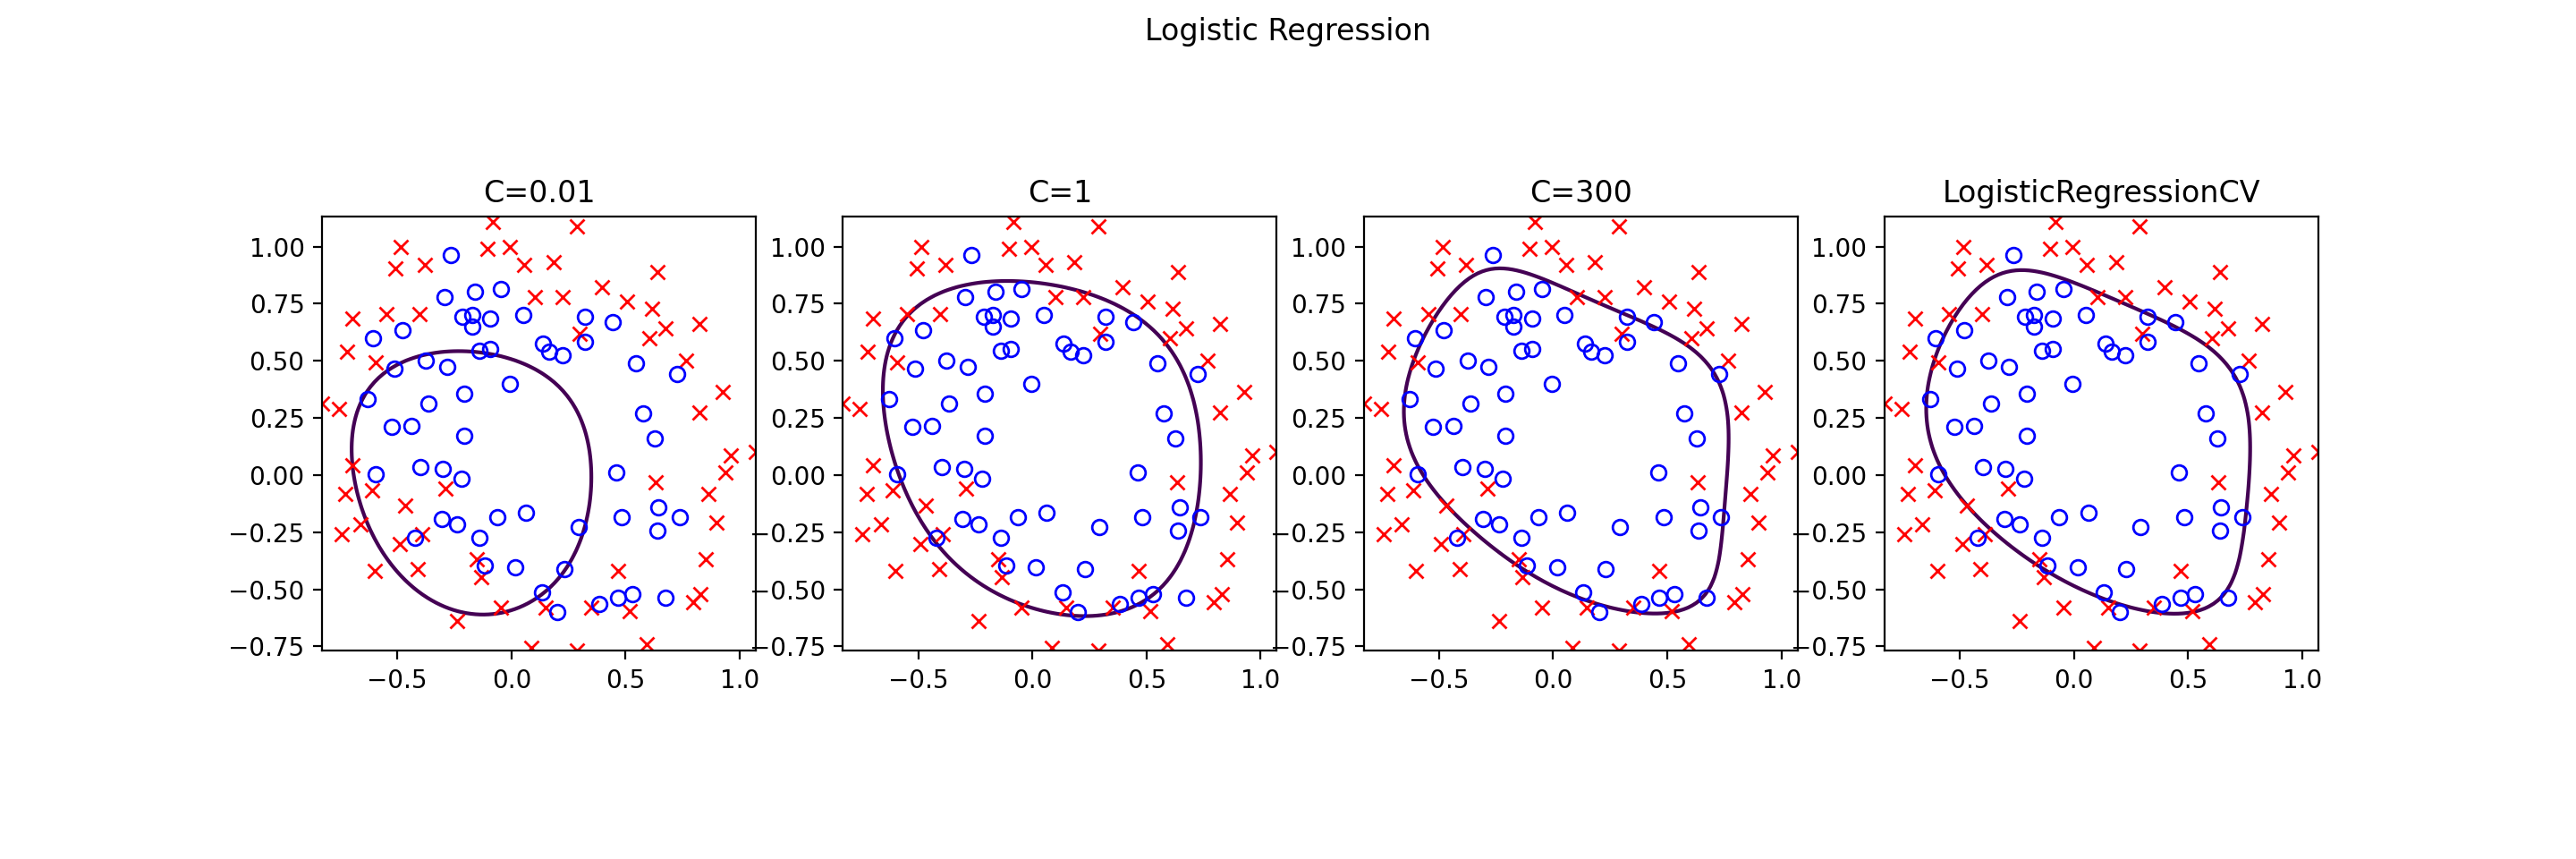
\includegraphics[width=\linewidth]{figs/Chap_15_LogisticRegression2.png}
\end{figure}

\paragraph{多项式回归}

\begin{center}
\begin{lstlisting}[language=Python]
"""
class sklearn.linear_model.Ridge(alpha=1.0, *, fit_intercept=True, normalize=False, 
copy_X=True, max_iter=None, tol=0.001, solver='auto', random_state=None)

class sklearn.preprocessing.PolynomialFeatures(degree=2, *, 
interaction_only=False, include_bias=True, order='C')
"""

import numpy as np
import matplotlib.pyplot as plt
from scipy.io import loadmat
from sklearn.linear_model import Ridge
from sklearn.linear_model import RidgeCV
from sklearn.preprocessing import PolynomialFeatures

data = loadmat('data/ex5data1.mat')
X = data['X']
y = data['y']
poly = PolynomialFeatures(degree=8)
newX = poly.fit_transform(X)

alphas = [0, 0.05, 10, -1]
fig, ax = plt.subplots(1, 4)
fig.suptitle('Polynomial Regression')
for i in range(4):
	alpha = alphas[i]
	if alpha == -1:
		reg = RidgeCV(normalize=True)
	else:
		reg = Ridge(alpha=alpha, normalize=True)
	reg.fit(newX, y)
	print(reg.score(newX, y))

	if alpha >= 0:
		ax[i].set_title('alpha={0}'.format(alpha))
	else:
		ax[i].set_title('RidgeCV')
	ax[i].plot(X.flatten(), y, 'x', color='red')
	ax[i].plot(np.linspace(X.min()-5, X.max()+5, 100), \
		reg.predict(poly.transform( np.linspace(X.min()-5, X.max()+5, 100).reshape((100, 1))) ))

plt.show()
\end{lstlisting}
\end{center}

\begin{figure}[H]
    \centering
    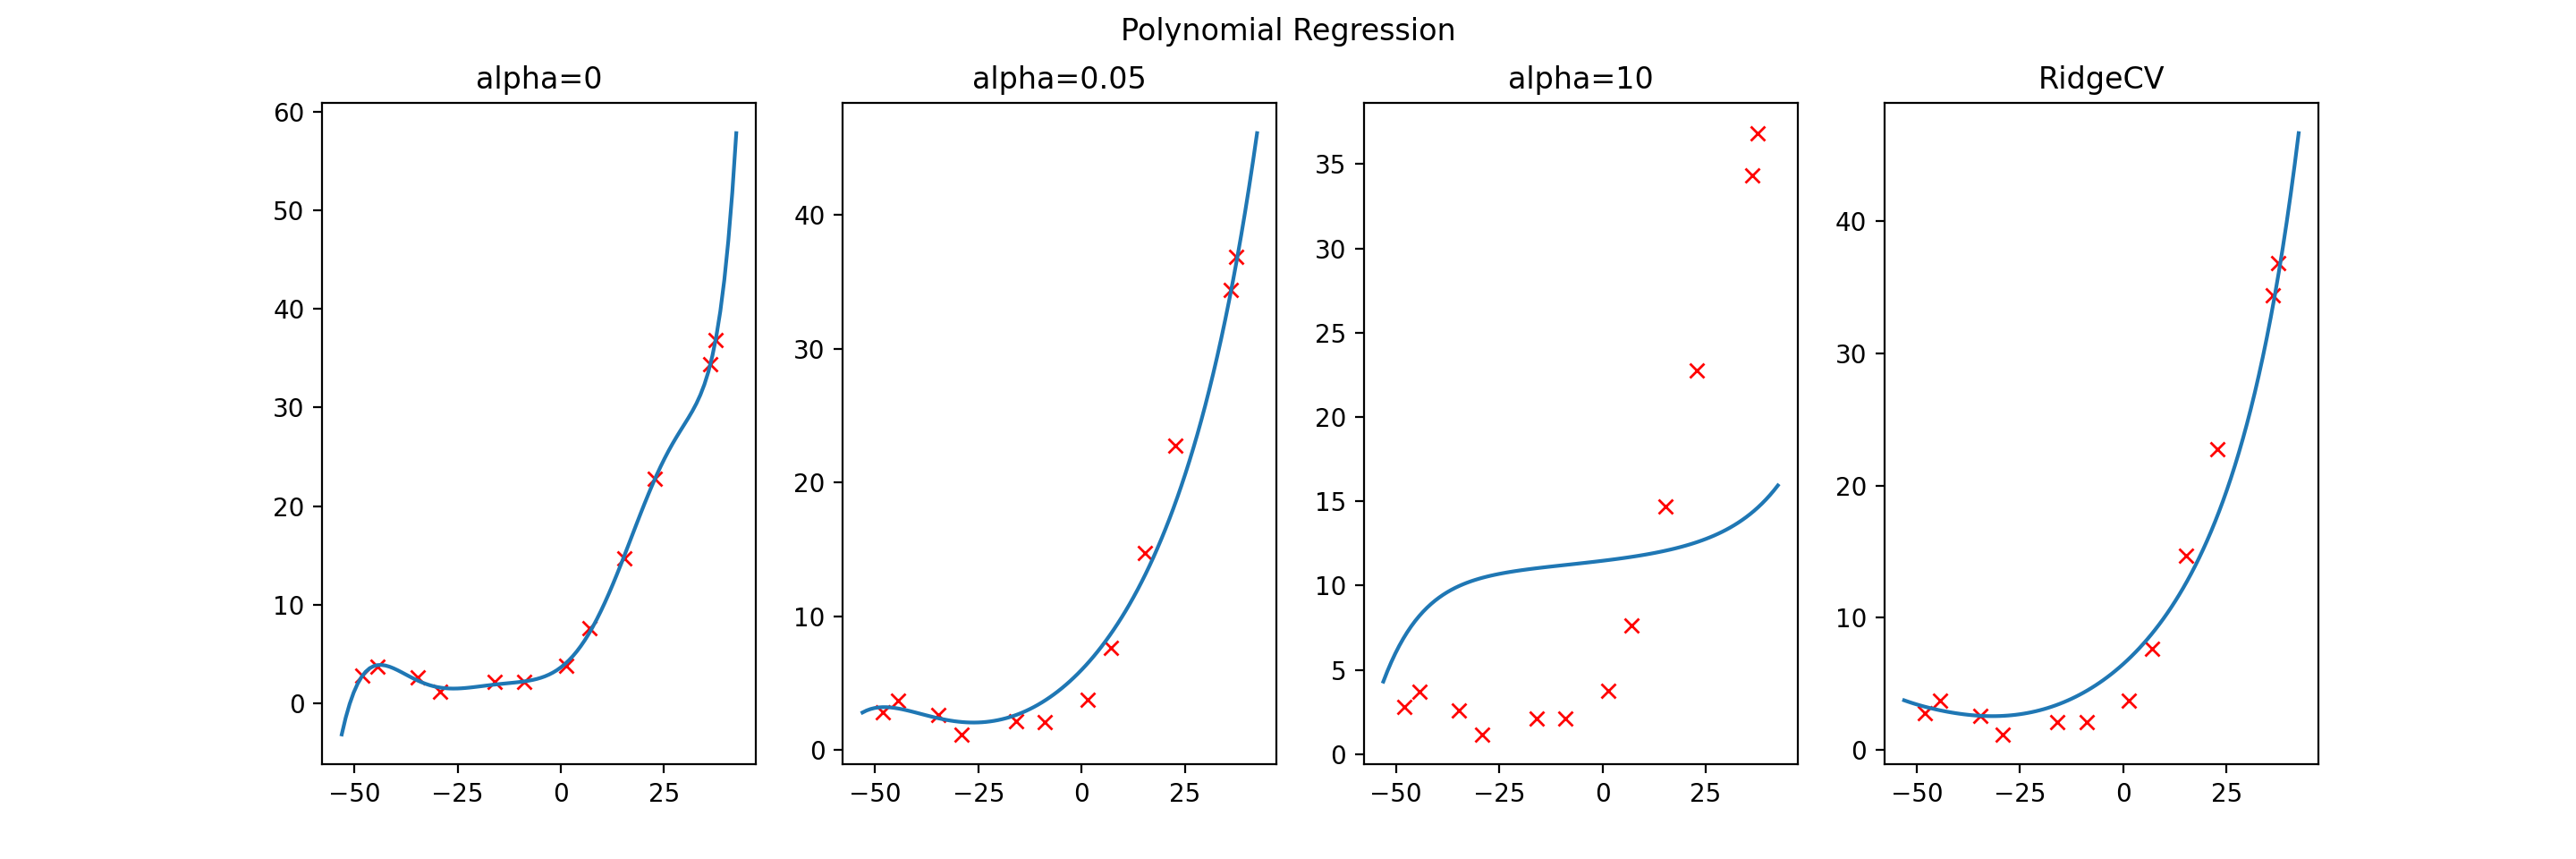
\includegraphics[width=\linewidth]{figs/Chap_15_PolynomialRegression.png}
\end{figure}


\paragraph{BP 神经网络}

\begin{center}
\begin{lstlisting}[language=Python]
"""
class sklearn.neural_network.MLPClassifier(hidden_layer_sizes=100, activation='relu', *, 
solver='adam', alpha=0.0001, batch_size='auto', learning_rate='constant', 
learning_rate_init=0.001, power_t=0.5, max_iter=200, shuffle=True, random_state=None, 
tol=0.0001, verbose=False, warm_start=False, momentum=0.9, nesterovs_momentum=True, 
early_stopping=False, validation_fraction=0.1, beta_1=0.9, beta_2=0.999, epsilon=1e-08, 
n_iter_no_change=10, max_fun=15000)
"""

import numpy as np
from scipy.io import loadmat
from sklearn.model_selection import train_test_split
from sklearn.neural_network import MLPClassifier

data = loadmat('data/ex4data1.mat')
X = data['X']
m = X.shape[0]
X = np.transpose(X.reshape(m, 20, 20), [0, 2, 1]).reshape(m, 400)
y = data['y']
y[y==10] = 0
y = y.flatten()
X_train, X_test, y_train, y_test = train_test_split(X, y, train_size = 0.8)

clf = MLPClassifier(hidden_layer_sizes=(25,), 
					random_state=True, 
					max_iter=1000)
clf.fit(X_train, y_train)
print(clf.score(X_test, y_test))
\end{lstlisting}
\end{center}

\paragraph{支持向量机}

\begin{center}
\begin{lstlisting}[language=Python]
"""
class sklearn.svm.LinearSVC(penalty='l2', loss='squared_hinge', *, dual=True, 
tol=0.0001, C=1.0, multi_class='ovr', fit_intercept=True, intercept_scaling=1, 
class_weight=None, verbose=0, random_state=None, max_iter=1000)
"""

import numpy as np
import matplotlib.pyplot as plt
from scipy.io import loadmat
from sklearn.svm import LinearSVC

data = loadmat('data/ex6data1.mat')
X = data['X']
y = data['y'].flatten()

Cs = [1, 100]
fig, ax = plt.subplots(1, 2)
fig.suptitle('LinearSVC')
x1, x2 = np.meshgrid(np.linspace(X[:, 0].min()-0.5, X[:, 0].max()+0.5, 100), 
	np.linspace(X[:, 1].min()-0.5, X[:, 1].max()+0.5, 100))
for i in range(2):
	C = Cs[i]
	clf = LinearSVC(C=C)
	clf.fit(X, y)
	print(clf.predict(X[:10]))

	ax[i].plot(X[y==0][:, 0], X[y==0][:, 1], 'x', color='red')
	ax[i].plot(X[y==1][:, 0], X[y==1][:, 1], 'o', color='blue')
	ax[i].contour(x1, x2, clf.decision_function(
		np.array([x1, x2]).transpose(1, 2, 0).reshape(10000, 2)
		).reshape(100, 100), [0])
	ax[i].set_xlabel('x1')
	ax[i].set_ylabel('x2')
	ax[i].set_title('C={0}'.format(C))
	ax[i].axis('square')

plt.show()
\end{lstlisting}
\end{center}

\begin{figure}[H]
    \centering
    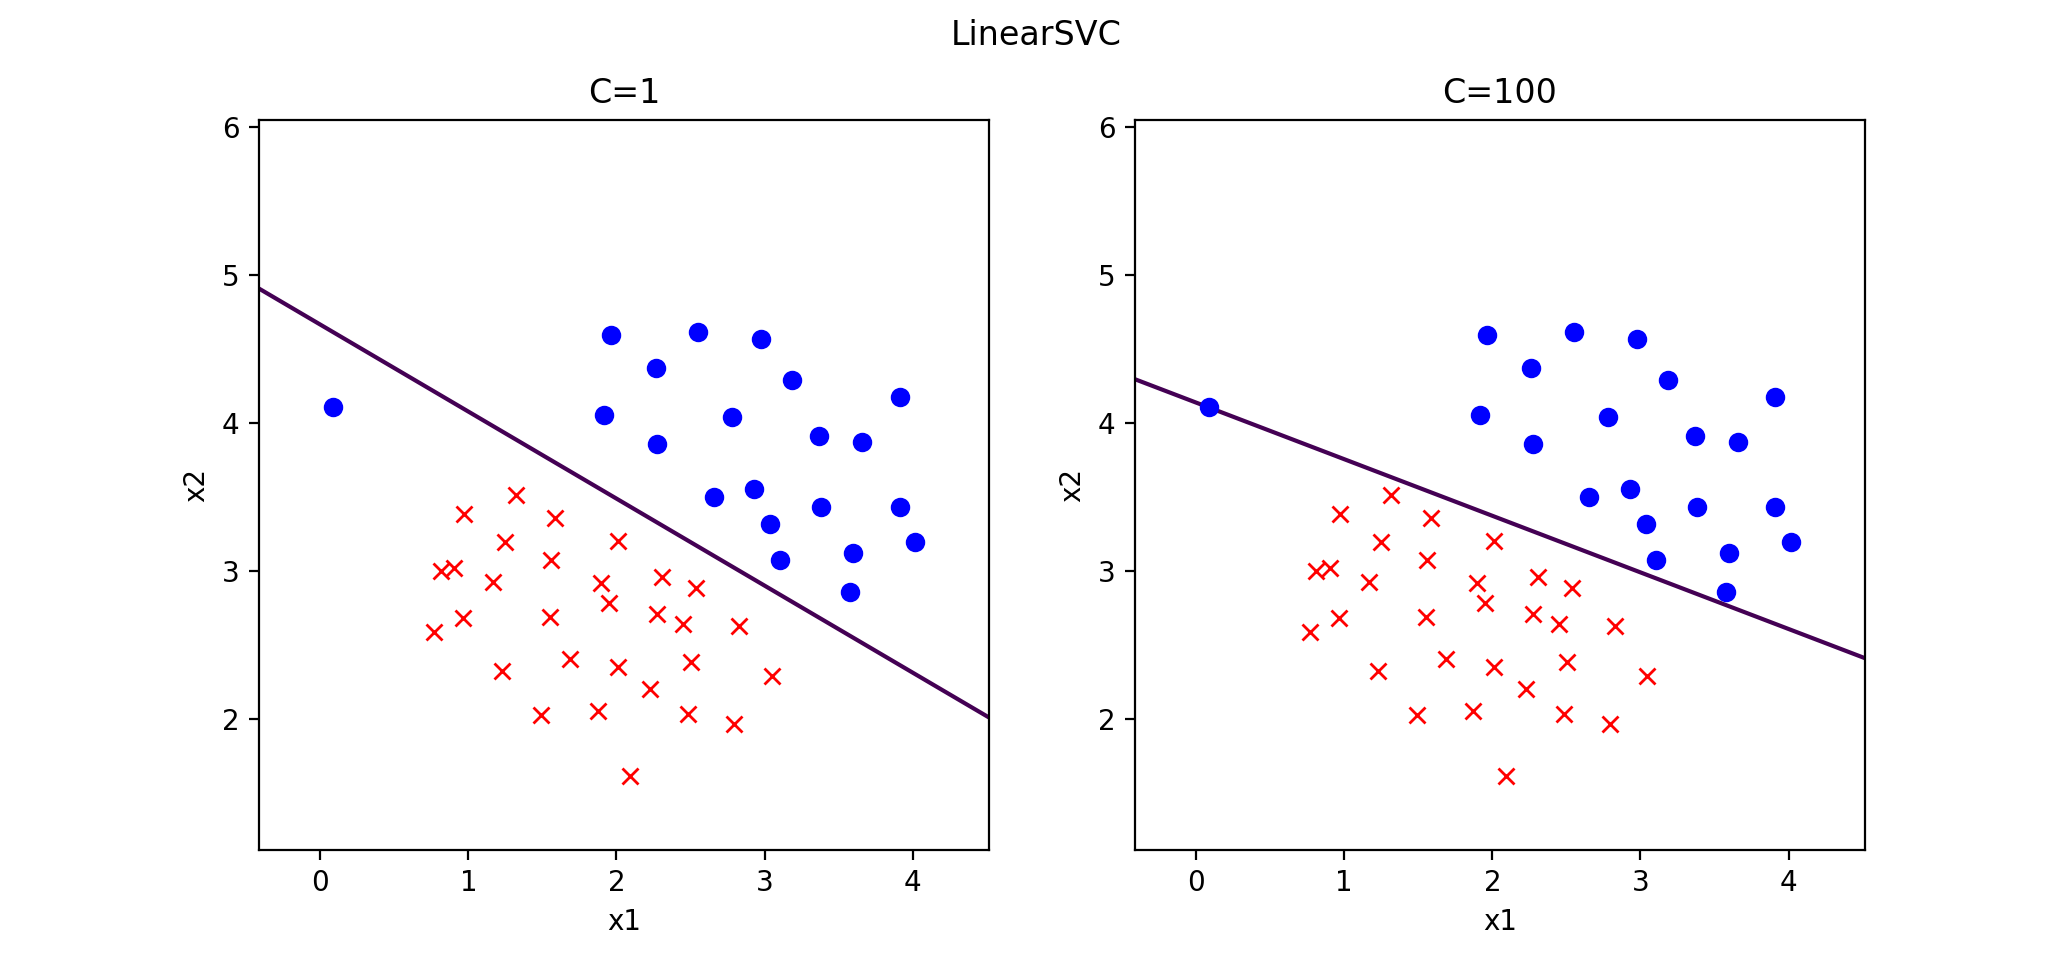
\includegraphics[width=\linewidth]{figs/Chap_15_LinearSVC.png}
\end{figure}

\begin{lstlisting}[language=Python]
"""
class sklearn.svm.SVC(*, C=1.0, kernel='rbf', degree=3, gamma='scale', 
coef0=0.0, shrinking=True, probability=False, tol=0.001, cache_size=200, 
class_weight=None, verbose=False, max_iter=- 1, decision_function_shape='ovr', 
break_ties=False, random_state=None)
"""

import numpy as np
import matplotlib.pyplot as plt
from scipy.io import loadmat
from sklearn.svm import SVC

data = loadmat('data/ex6data2.mat')
X = data['X']
y = data['y'].flatten()

Cs, gammas = [1, 100], [1, 10, 30]
fig, ax = plt.subplots(2, 3)
fig.suptitle('SVC')
x1, x2 = np.meshgrid(np.linspace(X[:, 0].min(), X[:, 0].max(), 100), 
	np.linspace(X[:, 1].min(), X[:, 1].max(), 100))
for i in range(2):
	for j in range(3):
		C, gamma = Cs[i], gammas[j]
		clf = SVC(C=C, kernel='rbf', probability=True, gamma=gamma)
		clf.fit(X, y)

		ax[i][j].plot(X[y==0][:, 0], X[y==0][:, 1], 'x', color='red', alpha=0.5)
		ax[i][j].plot(X[y==1][:, 0], X[y==1][:, 1], 'o', color='blue', markerfacecolor='none', alpha=0.5)
		ax[i][j].contour(x1, x2, clf.decision_function(
			np.array([x1, x2]).transpose(1, 2, 0).reshape(10000, 2)
			).reshape(100, 100), [0])
		ax[i][j].set_title('C={0}, gamma={1}'.format(C, gamma))

plt.show()
\end{lstlisting}

\begin{figure}[H]
    \centering
    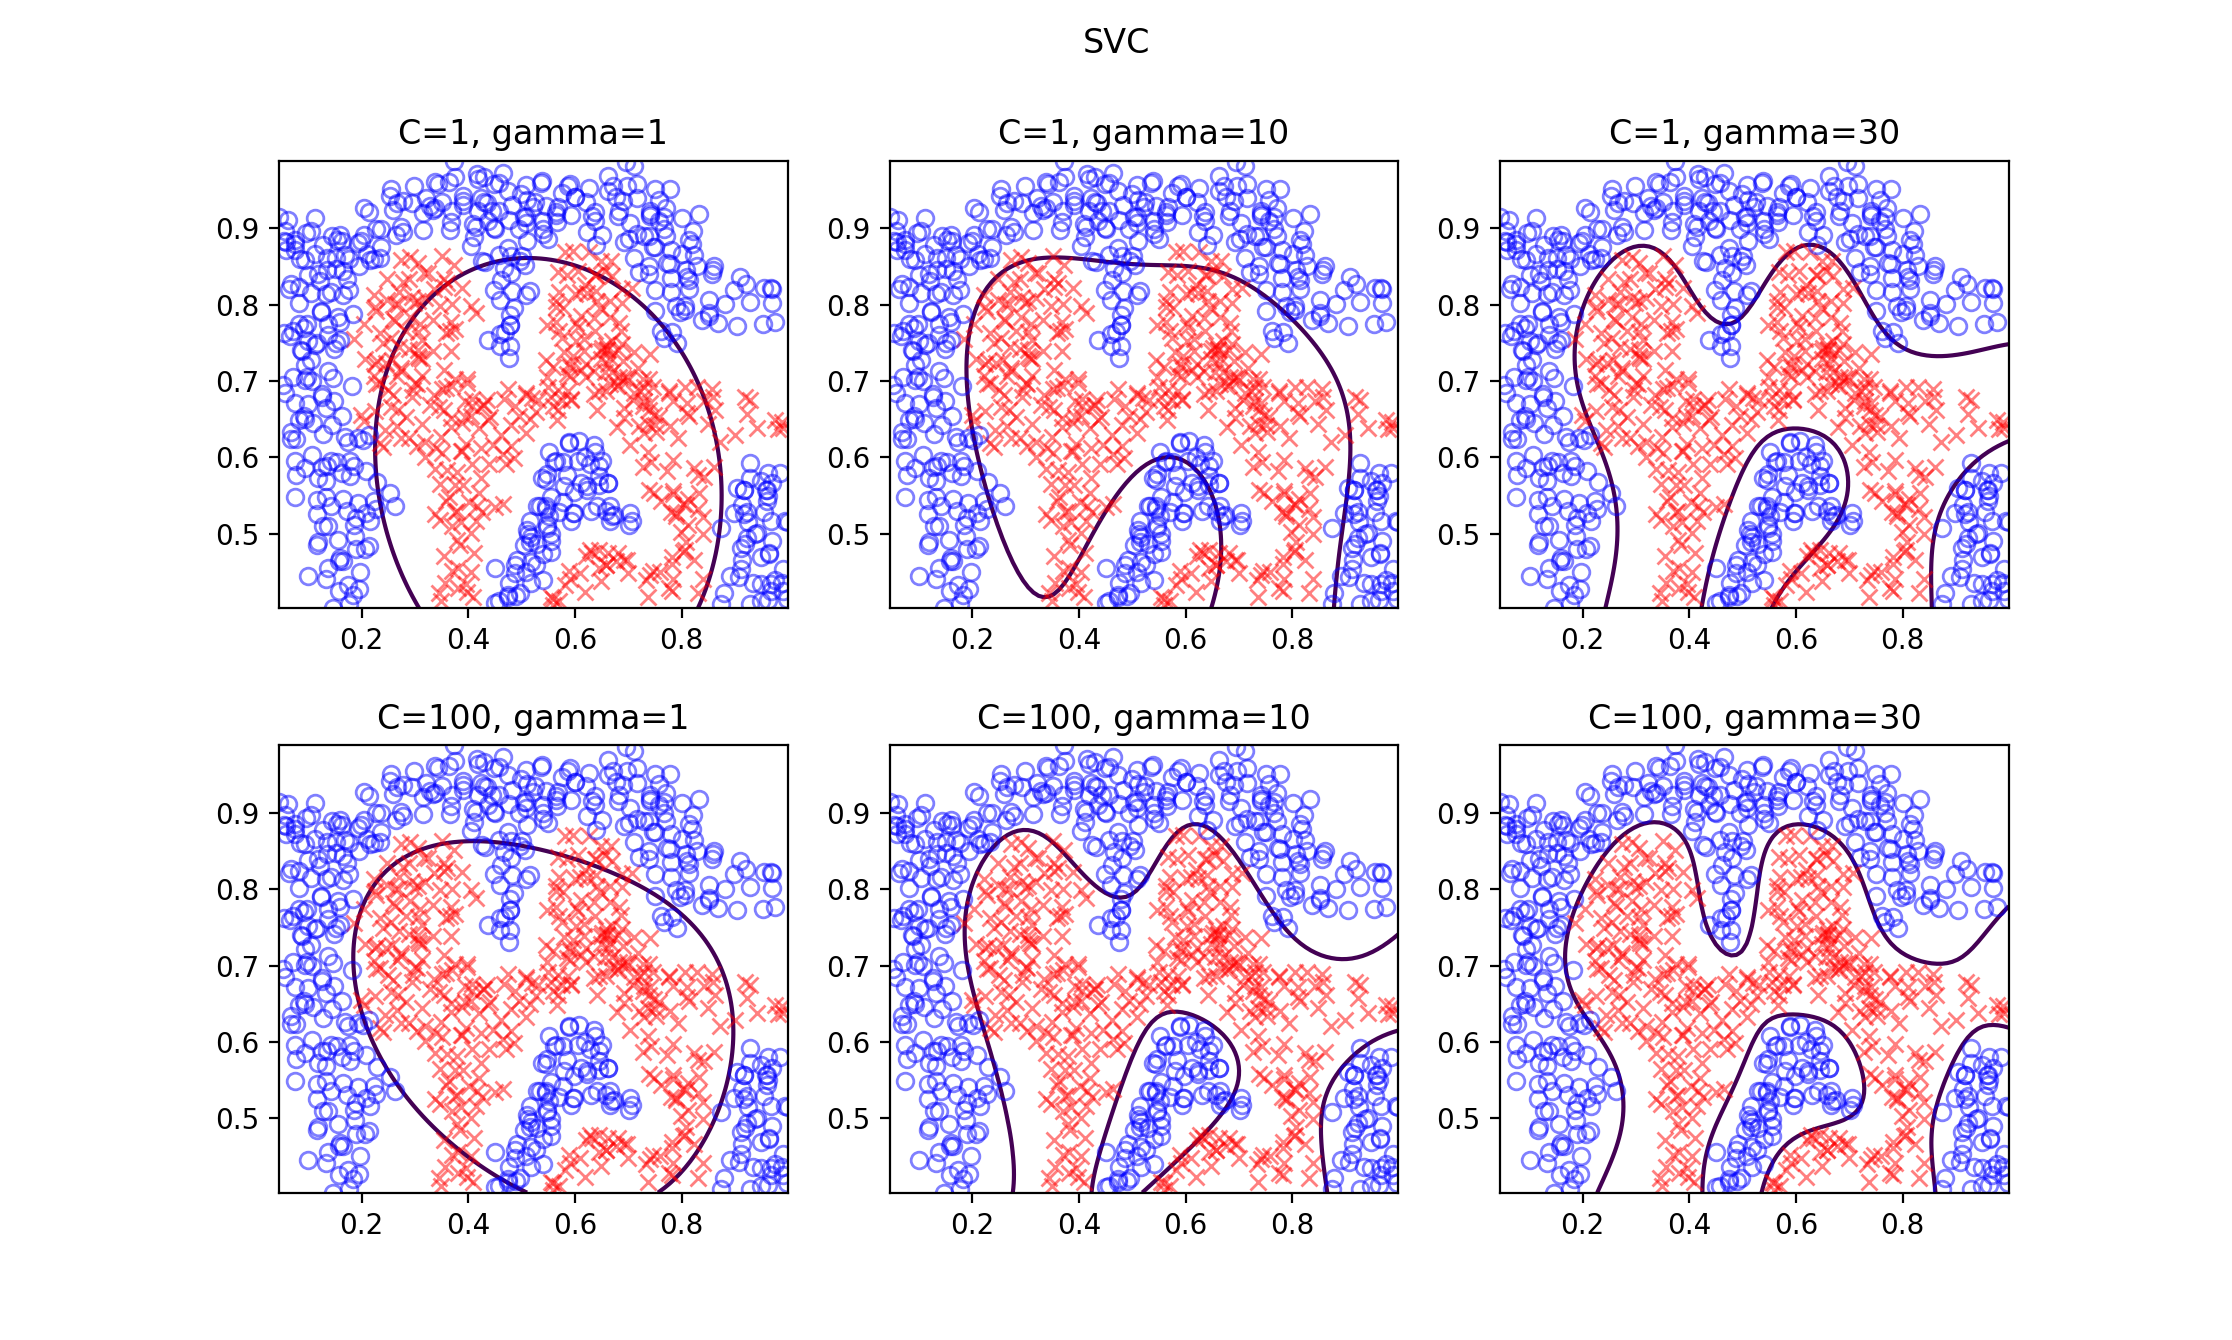
\includegraphics[width=\linewidth]{figs/Chap_15_SVC.png}
\end{figure}


\paragraph{K-Means}

\begin{center}
\begin{lstlisting}[language=Python]
"""
class sklearn.cluster.KMeans(n_clusters=8, *, init='k-means++', n_init=10, 
max_iter=300, tol=0.0001, precompute_distances='deprecated', verbose=0, 
random_state=None, copy_x=True, n_jobs='deprecated', algorithm='auto')
"""

import numpy as np
from scipy.io import loadmat
import matplotlib.pyplot as plt
from sklearn.cluster import KMeans

data = loadmat('data/ex7data2.mat')
X = data['X']

clt = KMeans(n_clusters=3)
belong = clt.fit_predict(X)

ax = plt.subplot(1, 1, 1)
ax.plot(X[belong==0][:, 0], X[belong==0][:, 1], 'o', color='blue', markerfacecolor='none')
ax.plot(X[belong==1][:, 0], X[belong==1][:, 1], 'o', color='red', markerfacecolor='none')
ax.plot(X[belong==2][:, 0], X[belong==2][:, 1], 'o', color='green', markerfacecolor='none')
ax.set_title('KMeans')
plt.show()
\end{lstlisting}
\end{center}

\begin{figure}[H]
    \centering
    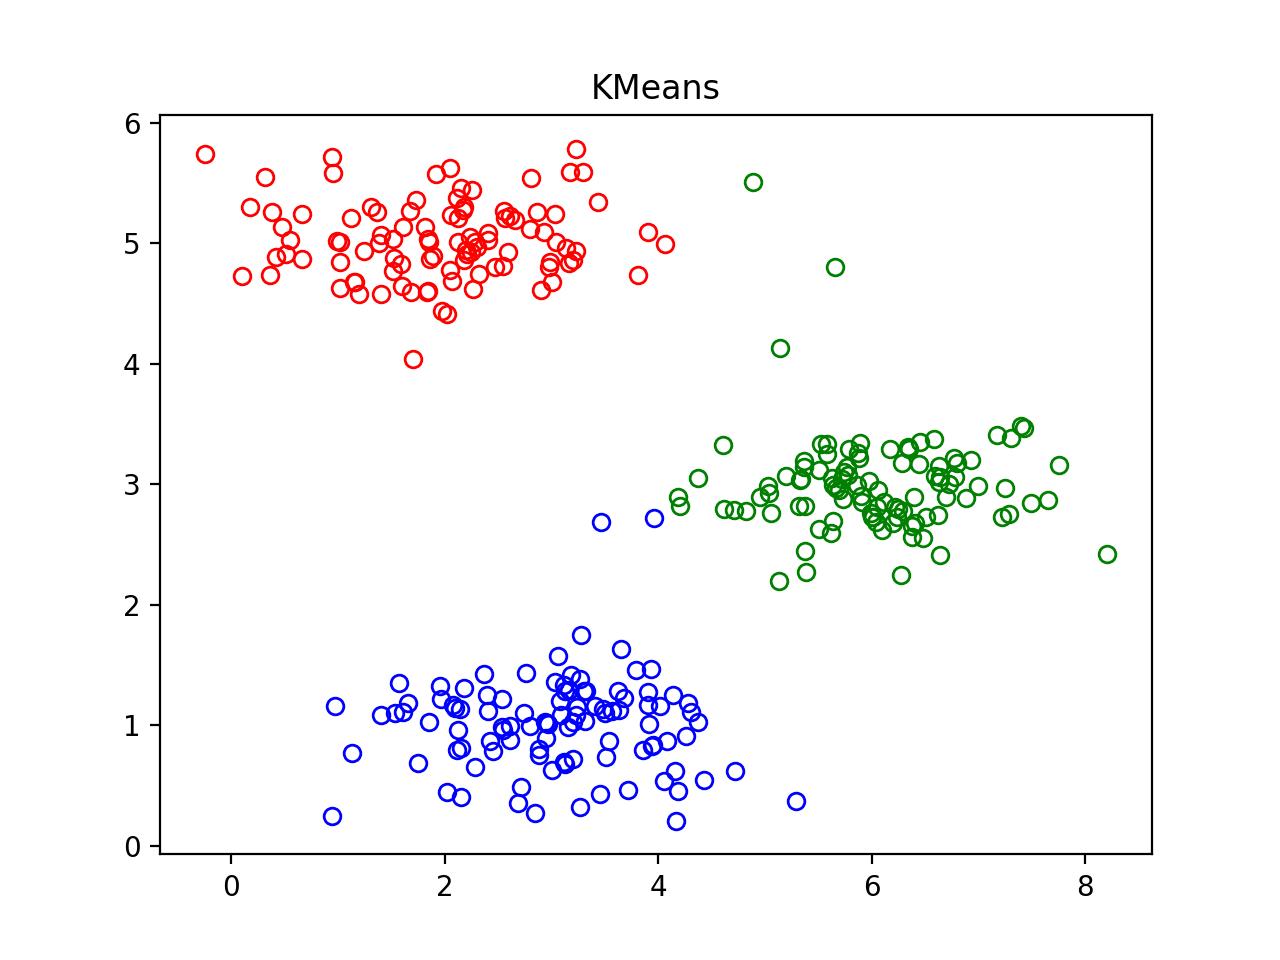
\includegraphics[width=0.5\linewidth]{figs/Chap_15_KMeans.png}
\end{figure}

\paragraph{主成分分析}

\begin{center}
\begin{lstlisting}[language=Python]
"""
class sklearn.decomposition.PCA(n_components=None, *, copy=True, whiten=False, 
svd_solver='auto', tol=0.0, iterated_power='auto', random_state=None)
"""

import numpy as np
from scipy.io import loadmat
import matplotlib.pyplot as plt
from sklearn.decomposition import PCA

data = loadmat('data/ex7data1.mat')
X = data['X']

pca = PCA(n_components=1)
pca.fit(X)
redX = pca.transform(X) # reduced X
recX = pca.inverse_transform(redX) # recovered X

ax = plt.subplot(1, 1, 1)
ax.plot(X[:, 0], X[:, 1], 'o', color='black', markerfacecolor='none')
ax.plot(recX[:, 0], recX[:, 1], 'o', color='red', markerfacecolor='none')
ax.set_title('PCA')
ax.axis('square')
plt.show()
\end{lstlisting}
\end{center}

\begin{figure}[H]
    \centering
    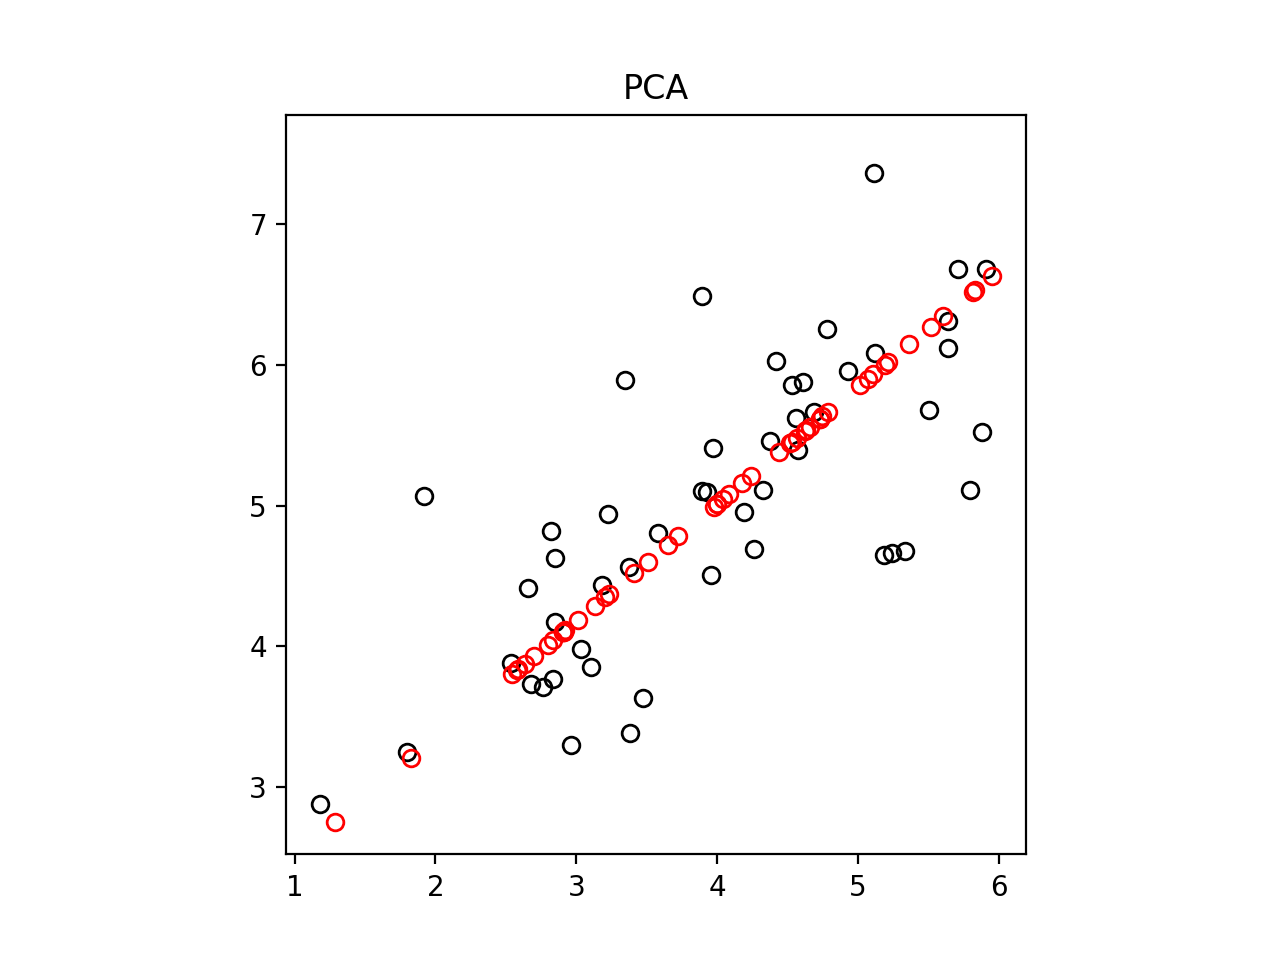
\includegraphics[width=0.5\linewidth]{figs/Chap_15_PCA.png}
\end{figure}

\begin{lstlisting}[language=Python]
"""
class sklearn.decomposition.PCA(n_components=None, *, copy=True, whiten=False, 
svd_solver='auto', tol=0.0, iterated_power='auto', random_state=None)
"""

import numpy as np
from scipy.io import loadmat
import matplotlib.pyplot as plt
import matplotlib
from sklearn.decomposition import PCA

X = loadmat('data/ex7faces.mat')['X']
X = np.transpose(X.reshape((5000, 32, 32)), [0, 2, 1]).reshape(5000, 1024)
X = -X

pca = PCA(n_components=0.99)
pca.fit(X)
redX = pca.transform(X) # reduced X
recX = pca.inverse_transform(redX) # recovered X

def show_a_face(face, ax):
	"""
	face.shape: (1024, )
	"""
	ax.matshow(face.reshape((32, 32)), cmap=matplotlib.cm.binary)
	ax.axis('off')

fig, ax = plt.subplots(5)
fig.suptitle('99% variance', fontweight='bold')
fig.subplots_adjust(hspace=0, wspace=None)
for i in range(5):
	show_a_face(recX[i], ax[i])
plt.show()
\end{lstlisting}

\begin{figure}[H]
    \centering
    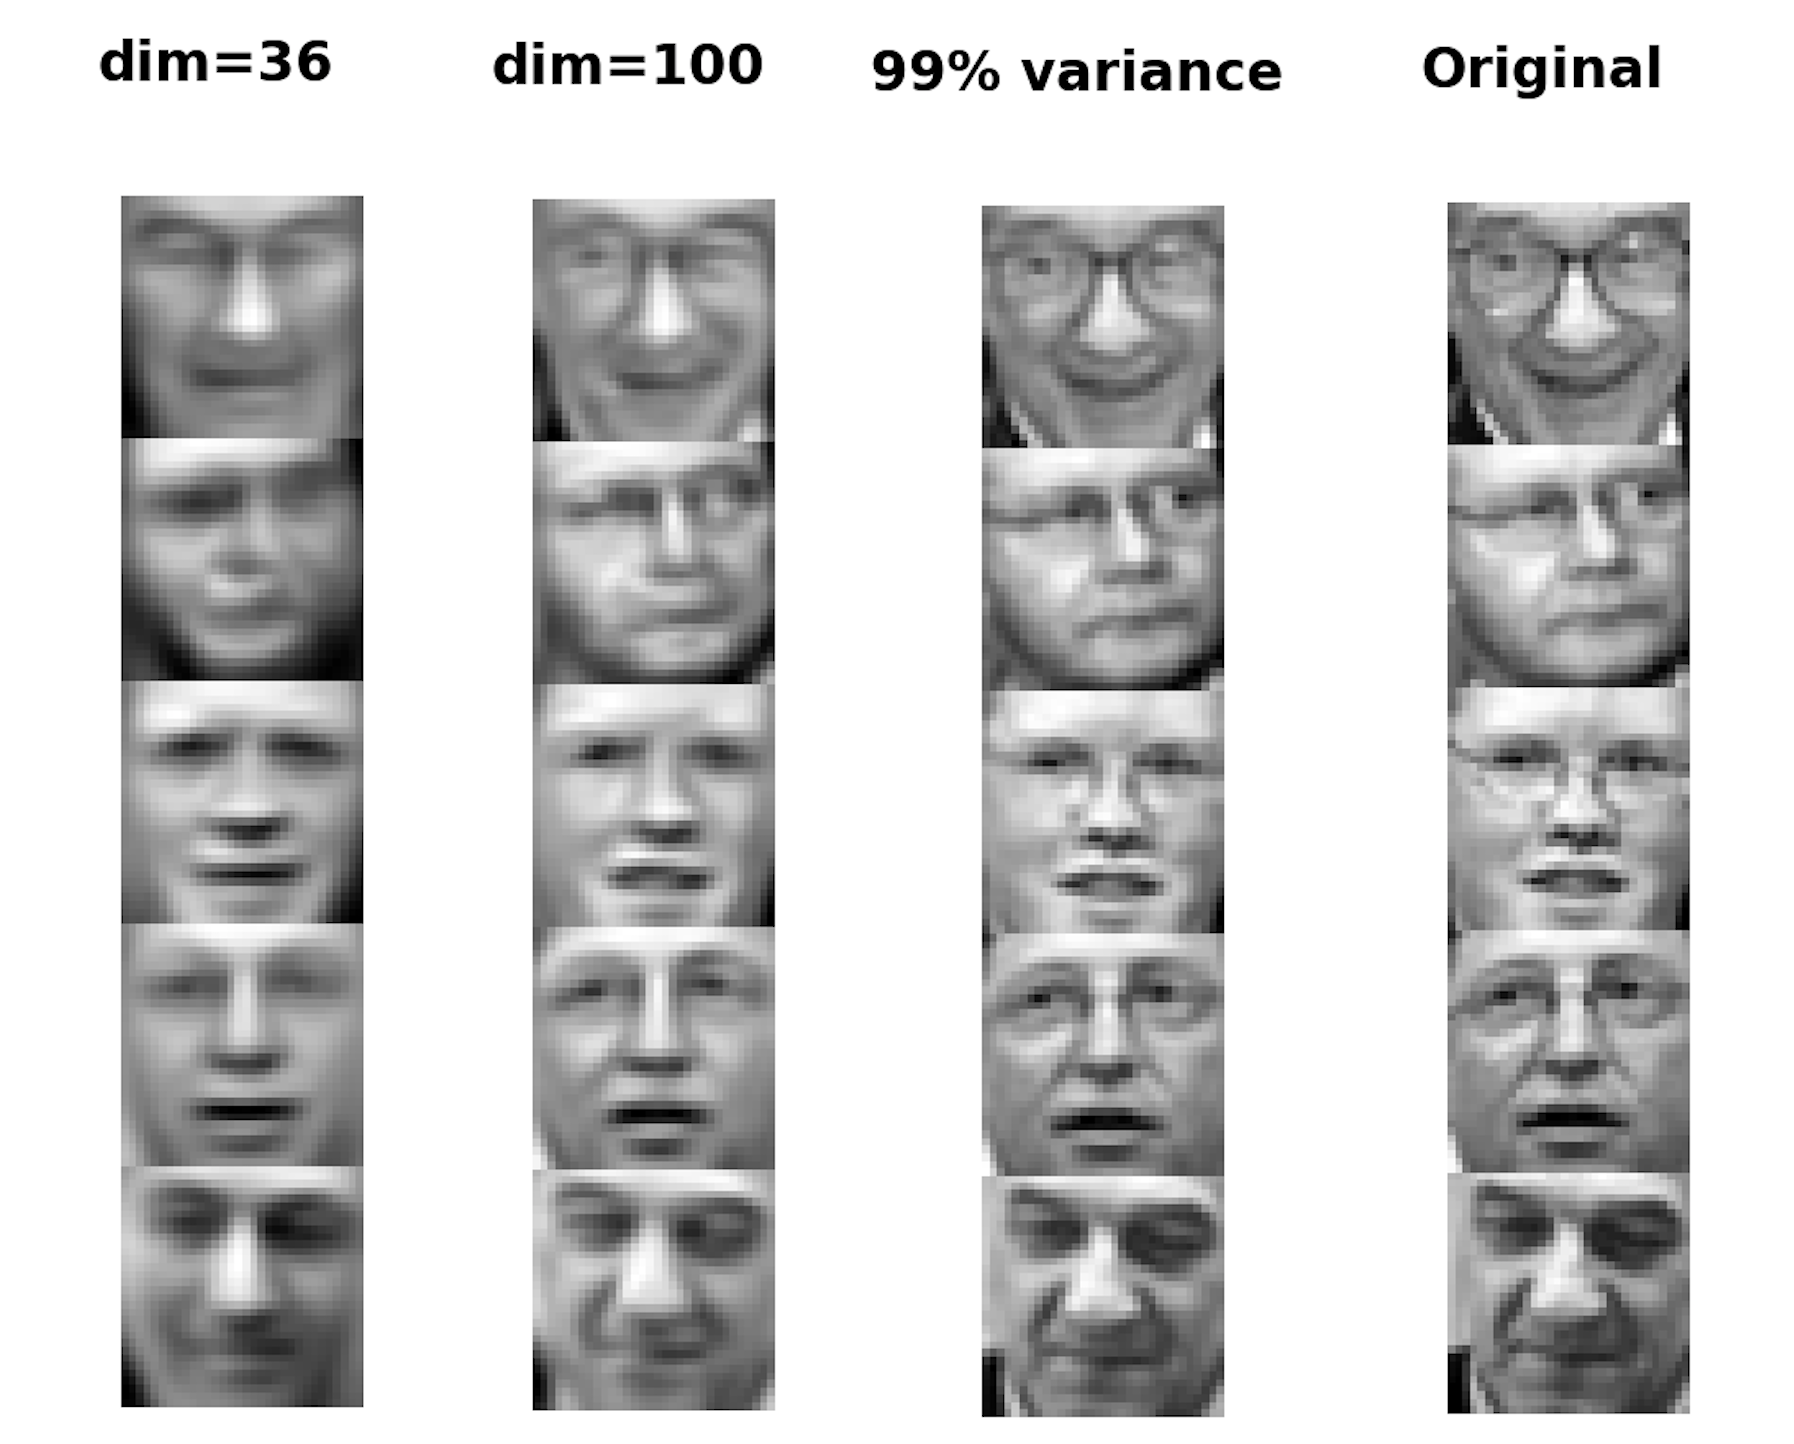
\includegraphics[width=0.5\linewidth]{figs/Chap_15_PCA2.png}
\end{figure}

\paragraph{异常检测}

\begin{center}
\begin{lstlisting}[language=Python]
"""
class sklearn.covariance.EllipticEnvelope(*, store_precision=True, assume_centered=False, 
support_fraction=None, contamination=0.1, random_state=None)

sklearn.metrics.f1_score(y_true, y_pred, *, labels=None, pos_label=1, 
average='binary', sample_weight=None, zero_division='warn')
"""

import numpy as np
from scipy.io import loadmat
from sklearn.covariance import EllipticEnvelope
from sklearn.metrics import f1_score
import matplotlib.pyplot as plt

data = loadmat('data/ex8data1.mat')
X, Xval, yval = data['X'], data['Xval'], data['yval'].flatten()

bestc, bestf1 = 0, 0
for c in np.linspace(0, 0.1, 100):
	ano = EllipticEnvelope(contamination=c)
	ano.fit(X)
	pred = ano.predict(X)
	pred[pred==1] = 0
	pred[pred==-1] = 1
	f1 = f1_score(yval, pred)
	if f1 > bestf1:
		bestc, bestf1 = c, f1

ano = EllipticEnvelope(contamination=bestc)
print(bestc)
ano.fit(X)
pred = ano.predict(X)

ax = plt.subplot(1, 1, 1)
ax.set_xlabel('Latency (ms)')
ax.set_ylabel('Throughput (mb/s)')
ax.plot(X[:, 0], X[:, 1], 'x', alpha=0.5, color='blue')
ax.plot(X[pred==-1][:, 0], X[pred==-1][:, 1], 'o', color='red', markerfacecolor='none', ms=10)
plt.show()
\end{lstlisting}
\end{center}

\begin{figure}[H]
    \centering
    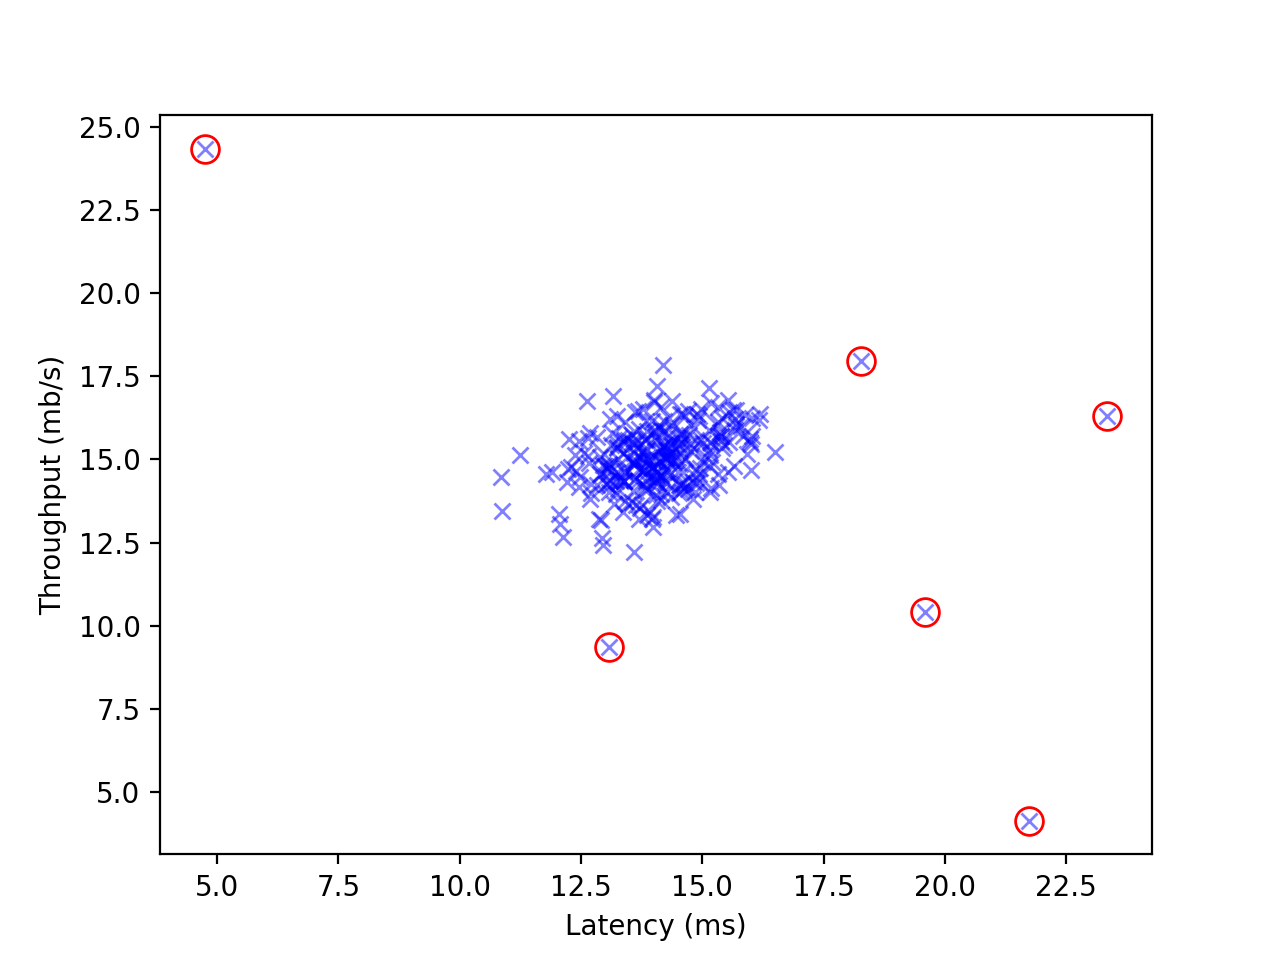
\includegraphics[width=0.5\linewidth]{figs/Chap_15_AnomalyDetection.png}
\end{figure}
 \newpage

\end{document}
